\section{Примеры}

Ниже приведены примеры работы программы для каждого из описанных в предыдущем разделе алгоритмов стабилизации и прочие пояснительные графики.
Для каждого из приведённых случаев, значения основных констант одинаково и равно
$$
	m = 2,\;
	\xi = 5,\;
	l = 10,\;
	g = 10,\;
	k = 2,\;
	M = 20.
$$
\null
\hfill
\begin{figure}[ht]
	\centering
	% This file was created by matlab2tikz.
%
%The latest updates can be retrieved from
%  http://www.mathworks.com/matlabcentral/fileexchange/22022-matlab2tikz-matlab2tikz
%where you can also make suggestions and rate matlab2tikz.
%
\definecolor{mycolor1}{rgb}{0.00000,0.44700,0.74100}%
%
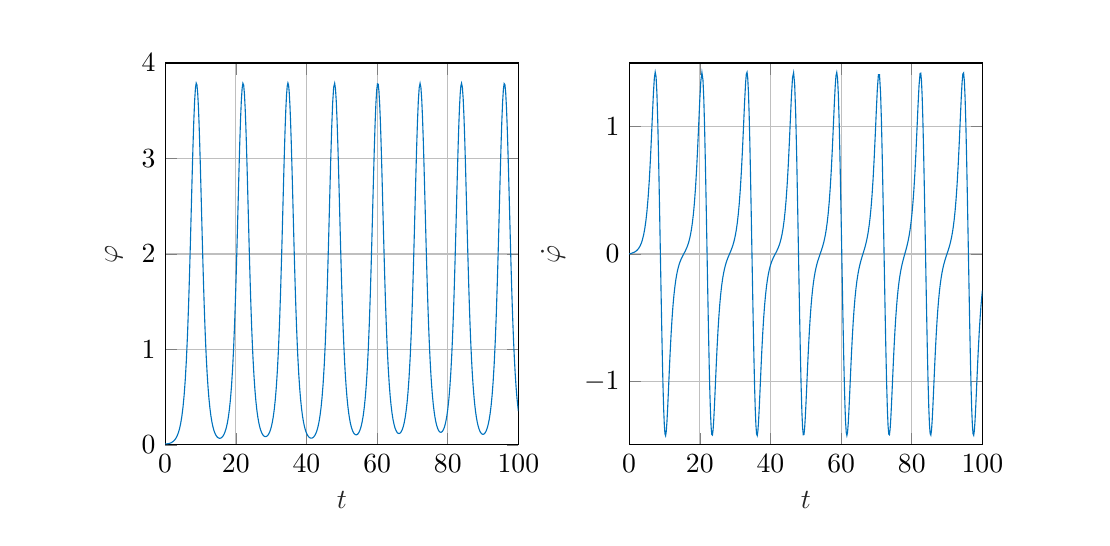
\begin{tikzpicture}

\begin{axis}[%
width=0.37\linewidth,
height=0.4\linewidth,
at={(0\linewidth,0\linewidth)},
scale only axis,
xmin=0,
xmax=100,
xlabel style={font=\color{white!15!black}},
xlabel={$t$},
ymin=0,
ymax=4,
ylabel style={font=\color{white!15!black}},
ylabel={$\varphi$},
axis background/.style={fill=white},
xmajorgrids,
ymajorgrids
]
\addplot [color=mycolor1, forget plot]
  table[row sep=crcr]{%
0	0.01\\
0.00669851267245177	0.0100001682595023\\
0.0133970253449035	0.0100006730436723\\
0.0200955380173553	0.0100015143694968\\
0.0267940506898071	0.0100026922652862\\
0.0602866140520659	0.0100136320725007\\
0.0937791774143248	0.0100329968904754\\
0.127271740776584	0.0100608030216901\\
0.160764304138842	0.0100970738518153\\
0.323329403895281	0.0103945328608821\\
0.485894503651719	0.0108983556105451\\
0.648459603408157	0.0116186788015832\\
0.811024703164596	0.0125697055755063\\
1.03948292252904	0.0143331786975851\\
1.26794114189348	0.0166590938052542\\
1.49639936125792	0.019639606381423\\
1.72485758062236	0.0233919550553814\\
2.00178626435616	0.0291900633840721\\
2.27871494808997	0.0366709033604124\\
2.55564363182377	0.0462701468389225\\
2.83257231555757	0.0585464222180734\\
3.14256554167497	0.0763467731571446\\
3.45255876779236	0.0996562160634277\\
3.76255199390976	0.130173335790394\\
4.07254522002715	0.170111866433466\\
4.39764108271027	0.225195185657921\\
4.72273694539339	0.298013323354906\\
5.04783280807651	0.394171235391819\\
5.37292867075962	0.52067704468804\\
5.69283484418233	0.68243399853175\\
6.01274101760503	0.891914589853088\\
6.33264719102772	1.1587658086657\\
6.65255336445043	1.48882989849951\\
6.89362536209534	1.77970915295561\\
7.13469735974025	2.10103378436983\\
7.37576935738516	2.44135421671588\\
7.61684135503007	2.7834005236591\\
7.85791335267498	3.10570301094522\\
8.09898535031989	3.38498670008805\\
8.34005734796481	3.60104224774233\\
8.58112934560972	3.7391720066544\\
8.79092964937004	3.78923177582674\\
9.00072995313036	3.77120261949345\\
9.21053025689068	3.68553822368727\\
9.420330560651	3.53676013753517\\
9.59928468692575	3.36576301519545\\
9.77823881320049	3.16088874034681\\
9.95719293947524	2.93012871997022\\
10.13614706575	2.68256701910148\\
10.3222258914073	2.41762380916675\\
10.5083047170645	2.1545813780885\\
10.6943835427218	1.90152503990877\\
10.8804623683791	1.66462836868281\\
11.0642647969712	1.45036962169653\\
11.2480672255633	1.2572050789395\\
11.4318696541554	1.08544370465712\\
11.6156720827476	0.934411058187077\\
11.8748760021579	0.75359465097649\\
12.1340799215681	0.606059445724902\\
12.3932838409784	0.486948655069062\\
12.6524877603887	0.39125593064464\\
12.9219218246881	0.31161456589316\\
13.1913558889875	0.248717623544482\\
13.4607899532869	0.199517411070746\\
13.7302240175863	0.16113567714543\\
13.9603385792327	0.135164552416587\\
14.190453140879	0.114572412616805\\
14.4205677025254	0.0985810679478034\\
14.6506822641717	0.0865079723859402\\
14.8750119013515	0.0780104447553899\\
15.0993415385313	0.0724679087290245\\
15.3236711757111	0.0696847501659681\\
15.548000812891	0.0695372364895898\\
15.7574813344118	0.0717580714277425\\
15.9669618559326	0.0763447608416404\\
16.1764423774534	0.083452662870547\\
16.3859228989742	0.0933114748279183\\
16.6221572617536	0.108133544442442\\
16.8583916245331	0.127481454539233\\
17.0946259873126	0.152166868269979\\
17.3308603500921	0.183214839767316\\
17.613981472634	0.23060992204736\\
17.897102595176	0.291756214074516\\
18.1802237177179	0.37020443194941\\
18.4633448402599	0.470332055261299\\
18.7696311379685	0.608806737250182\\
19.0759174356772	0.787087117959642\\
19.3822037333858	1.01376500537075\\
19.6884900310945	1.29577966270822\\
19.9914955456333	1.63306879014673\\
20.2945010601721	2.02334700844075\\
20.5975065747109	2.44826086740783\\
20.9005120892497	2.87518207733491\\
21.1211577443938	3.16258892699062\\
21.341803399538	3.41053312872327\\
21.5624490546822	3.60397187103186\\
21.7830947098264	3.73198934068656\\
22.0037403649706	3.78818630769374\\
22.2243860201147	3.76913744749188\\
22.4450316752589	3.67529745371577\\
22.6656773304031	3.51220688668443\\
22.8468598510926	3.33313069700488\\
23.0280423717821	3.12064997670467\\
23.2092248924716	2.88327352333772\\
23.3904074131612	2.63053223415612\\
23.5758773479812	2.36623208795007\\
23.7613472828012	2.10553502410004\\
23.9468172176212	1.8560745640241\\
24.1322871524412	1.62354562922104\\
24.3178195301611	1.41138459742705\\
24.5033519078811	1.22087064330735\\
24.6888842856011	1.05207960573426\\
24.8744166633211	0.904148060660449\\
25.1409406392388	0.724679449152889\\
25.4074646151566	0.579422488935479\\
25.6739885910744	0.463176500136162\\
25.9405125669921	0.370617129641398\\
26.2054834530332	0.297269148711034\\
26.4704543390743	0.239395646188422\\
26.7354252251153	0.194264337845412\\
27.0003961111564	0.159322584392641\\
27.2297541458232	0.135724989183033\\
27.4591121804899	0.117491720653848\\
27.6884702151567	0.103940527502074\\
27.9178282498234	0.0944928573178351\\
28.1397074559272	0.0888686873424555\\
28.361586662031	0.0865342785264056\\
28.5834658681348	0.0874159141925233\\
28.8053450742386	0.0915303003148161\\
29.0011538063346	0.0979527233606929\\
29.1969625384306	0.107192115153624\\
29.3927712705265	0.119515952328061\\
29.5885800026225	0.135275024258959\\
29.8398914310286	0.161264720758223\\
30.0912028594348	0.194870453725322\\
30.3425142878409	0.237667962629424\\
30.593825716247	0.291631380573633\\
30.8864683323523	0.371730110963118\\
31.1791109484576	0.475115859659639\\
31.4717535645629	0.607698520359995\\
31.7643961806682	0.776201785930627\\
32.0662076690762	0.994721258525719\\
32.3680191574842	1.26741489907583\\
32.6698306458922	1.59809253083388\\
32.9716421343002	1.98206534013354\\
33.1707822354883	2.25779599710058\\
33.3699223366764	2.54144401277206\\
33.5690624378645	2.82209207398526\\
33.7682025390526	3.08735098724502\\
33.9673426402407	3.32438112549048\\
34.1664827414288	3.52135920822987\\
34.3656228426169	3.66864802711774\\
34.564762943805	3.75971887453594\\
34.7529686722052	3.79086304280623\\
34.9411744006054	3.76713600477374\\
35.1293801290056	3.68923768904417\\
35.3175858574058	3.56039047950655\\
35.5057915858061	3.3859191102897\\
35.6939973142063	3.1731269001796\\
35.8822030426065	2.93115060622488\\
36.0704087710067	2.670533191756\\
36.2569704793276	2.40478954000857\\
36.4435321876484	2.14139453882823\\
36.6300938959693	1.88839989604263\\
36.8166556042901	1.65191262733024\\
37.0008196717549	1.43843551034908\\
37.1849837392198	1.24618778026176\\
37.3691478066846	1.07540672651605\\
37.5533118741494	0.925361982807363\\
37.8146645067	0.74485017797357\\
38.0760171392507	0.597893513740105\\
38.3373697718013	0.479529497760531\\
38.5987224043519	0.384653272006509\\
38.8667896548655	0.306796545926677\\
39.1348569053791	0.245268173126148\\
39.4029241558926	0.197109042667227\\
39.6709914064062	0.159530920156519\\
39.900939606894	0.134014690972985\\
40.1308878073818	0.113824207049912\\
40.3608360078696	0.0981975760228951\\
40.5907842083574	0.0864683931618888\\
40.8148883177155	0.0783023779761507\\
41.0389924270735	0.0730962343200021\\
41.2630965364315	0.0706672202450362\\
41.4872006457896	0.0709055916885004\\
41.6955568258498	0.0735119715927551\\
41.9039130059099	0.0785157625416213\\
42.1122691859701	0.0860840659988296\\
42.3206253660303	0.0964592804118289\\
42.5588461230691	0.112193139197327\\
42.7970668801078	0.132701189904611\\
43.0352876371466	0.158857622074721\\
43.2735083941853	0.191765822855492\\
43.5579480692047	0.241825434278239\\
43.842387744224	0.306424638259814\\
44.1268274192433	0.38933119387794\\
44.4112670942627	0.495170233181422\\
44.7174610278787	0.640685066078484\\
45.0236549614947	0.827689505158457\\
45.3298488951107	1.06474500451225\\
45.6360428287267	1.3582393028508\\
45.9409076945358	1.7092860931246\\
46.245772560345	2.11126606150897\\
46.5506374261542	2.5424321756521\\
46.8555022919633	2.96677736976667\\
47.1379987211111	3.3151496220636\\
47.420495150259	3.58411440624506\\
47.7029915794068	3.74623254485524\\
47.9854880085546	3.78728363696202\\
48.2148328536182	3.73025135313108\\
48.4441776986818	3.59524942274679\\
48.6735225437453	3.38977377288643\\
48.9028673888089	3.12705378628534\\
49.0958013016488	2.87446068001518\\
49.2887352144886	2.60507138247999\\
49.4816691273285	2.33026760564412\\
49.6746030401683	2.06051861905989\\
49.85195947436	1.82454280463563\\
50.0293159085517	1.60446165158843\\
50.2066723427433	1.40302362282019\\
50.384028776935	1.22154052610654\\
50.5996947885122	1.02762698554767\\
50.8153608000894	0.861428828398503\\
51.0310268116666	0.720525077896423\\
51.2466928232438	0.602007613653801\\
51.4799367507515	0.495375781323717\\
51.7131806782591	0.407932364322021\\
51.9464246057668	0.336724998675276\\
52.1796685332745	0.278968327945056\\
52.4129124607822	0.232270380151798\\
52.6461563882898	0.194992153847793\\
52.8794003157975	0.165718111090892\\
53.1126442433052	0.143186190001923\\
53.3397605791066	0.126780067039686\\
53.5668769149081	0.115286925242566\\
53.7939932507095	0.108289846301111\\
54.0211095865109	0.105484591834511\\
54.2354379899311	0.106554449495601\\
54.4497663933514	0.111298114057187\\
54.6640947967716	0.119886813284953\\
54.8784232001918	0.132605979807753\\
55.1059320672162	0.151104507362789\\
55.3334409342406	0.175454251676556\\
55.560949801265	0.206594117112438\\
55.7884586682894	0.245706987320803\\
56.0658263305795	0.306304199198775\\
56.3431939928697	0.384283371278622\\
56.6205616551598	0.483828770346586\\
56.8979293174499	0.60992977426013\\
57.1986917409398	0.782878420524803\\
57.4994541644297	1.00242998552612\\
57.8002165879196	1.27584523814164\\
58.1009790114095	1.60602886726603\\
58.3234349457233	1.8852633360136\\
58.5458908800371	2.18778038348945\\
58.7683468143509	2.50314941861488\\
58.9908027486648	2.81691800339631\\
59.2132586829786	3.11185271684344\\
59.4357146172924	3.36976921634192\\
59.6581705516062	3.57477569854162\\
59.88062648592	3.71498489644668\\
60.0946418448988	3.78181795281938\\
60.3086572038775	3.77816362044307\\
60.5226725628562	3.70373880659392\\
60.7366879218349	3.56270594523158\\
60.9146591015628	3.4001554100017\\
61.0926302812907	3.20276428918516\\
61.2706014610186	2.97812328046305\\
61.4485726407465	2.73501222625391\\
61.6352665051391	2.47040938230448\\
61.8219603695316	2.20587388360019\\
62.0086542339241	1.94992449084112\\
62.1953480983167	1.70922063981204\\
62.3776188933813	1.493191467031\\
62.559889688446	1.2976868645459\\
62.7421604835107	1.12327386862497\\
62.9244312785753	0.969492223205636\\
63.1768453388234	0.787975249865612\\
63.4292593990716	0.639017305639627\\
63.6816734593197	0.518147780186055\\
63.9340875195678	0.420725660690642\\
64.2090253010309	0.336158363631927\\
64.483963082494	0.270335444388343\\
64.7589008639571	0.219989508915525\\
65.0338386454202	0.182046746958196\\
65.2638721466347	0.158062708889788\\
65.4939056478493	0.140351907733185\\
65.7239391490638	0.128254913307769\\
65.9539726502784	0.121245661743849\\
66.1726186752786	0.119004812435739\\
66.3912647002788	0.121033234017409\\
66.609910725279	0.127415633096882\\
66.8285567502793	0.138364962751572\\
67.0423874862799	0.153849320506751\\
67.2562182222806	0.17459458504719\\
67.4700489582813	0.201307284619366\\
67.6838796942819	0.234883031415822\\
67.952145217326	0.288429674623165\\
68.2204107403701	0.357316435632235\\
68.4886762634141	0.445037479041028\\
68.7569417864582	0.555804056824633\\
69.0552368695642	0.711645030263095\\
69.3535319526702	0.910216730104028\\
69.6518270357763	1.15913102132564\\
69.9501221188823	1.46309695454496\\
70.2557768156964	1.83202037402632\\
70.5614315125106	2.24671971691534\\
70.8670862093247	2.68065543859719\\
71.1727409061389	3.09390293547\\
71.4206744352764	3.38179831633751\\
71.668607964414	3.60343070485978\\
71.9165414935515	3.74167316408411\\
72.1644750226891	3.7874384049651\\
72.3985854735263	3.74420933735991\\
72.6326959243636	3.61890531172263\\
72.8668063752009	3.4186225239476\\
73.1009168260381	3.15678976262403\\
73.294064307944	2.90721185345251\\
73.4872117898498	2.63932786094604\\
73.6803592717556	2.36460080630771\\
73.8735067536614	2.09371891937535\\
74.0512448032496	1.85567696935556\\
74.2289828528378	1.63309062544149\\
74.406720902426	1.42895315588612\\
74.5844589520142	1.24477501434217\\
74.7977288538951	1.05021349368448\\
75.010998755776	0.883011702679233\\
75.2242686576569	0.740919685724049\\
75.4375385595378	0.621175620148695\\
75.67197806715	0.511697298944302\\
75.9064175747622	0.422164944963326\\
76.1408570823744	0.34956093849779\\
76.3752965899866	0.291037493804999\\
76.6097360975988	0.244154362283524\\
76.844175605211	0.20726134874291\\
77.0786151128232	0.178951900651768\\
77.3130546204354	0.157991168973219\\
77.5391823766931	0.143856944982067\\
77.7653101329507	0.135241038906622\\
77.9914378892084	0.131841044418962\\
78.2175656454661	0.133494320353473\\
78.4250959850965	0.139482870526184\\
78.632626324727	0.149969792076237\\
78.8401566643575	0.165297354851603\\
79.0476870039879	0.185947824595166\\
79.2904620782681	0.217738564668648\\
79.5332371525482	0.259080985364617\\
79.7760122268284	0.311751779859784\\
80.0187873011085	0.37795628413527\\
80.3056971394969	0.477217780721438\\
80.5926069778852	0.604665852434664\\
80.8795168162735	0.766691519298677\\
81.1664266546618	0.96995031840188\\
81.4639747879115	1.23067240247887\\
81.7615229211611	1.5476370267611\\
82.0590710544107	1.91813181614511\\
82.3566191876603	2.32804808677477\\
82.5503324233063	2.60402749972104\\
82.7440456589523	2.87453760272862\\
82.9377588945983	3.12792653050532\\
83.1314721302443	3.35272612522543\\
83.3251853658902	3.53849845296068\\
83.5188986015362	3.67673226101255\\
83.7126118371822	3.76121050715506\\
83.9063250728282	3.78868056670258\\
84.1361863249589	3.74666819792617\\
84.3660475770895	3.62538155957218\\
84.5959088292202	3.4314475601377\\
84.8257700813509	3.17736452807888\\
85.017992604011	2.93090403513616\\
85.2102151266711	2.6652495561901\\
85.4024376493312	2.39174569412114\\
85.5946601719913	2.12107566924645\\
85.7727145105963	1.88090382040442\\
85.9507688492014	1.6558079980321\\
86.1288231878065	1.44898879996104\\
86.3068775264116	1.26212194080477\\
86.5181412284744	1.06653447767585\\
86.7294049305373	0.897963365743336\\
86.9406686326001	0.754275973521599\\
87.151932334663	0.632803962771961\\
87.3879159319866	0.519714152558152\\
87.6238995293101	0.427110143970677\\
87.8598831266337	0.351847052215549\\
88.0958667239573	0.290940486800345\\
88.3318503212809	0.241817399031119\\
88.5678339186044	0.202724220106999\\
88.803817515928	0.172148015948917\\
89.0398011132516	0.148738340274585\\
89.2670082487296	0.13198363616301\\
89.4942153842076	0.120345954424\\
89.7214225196856	0.113403710305463\\
89.9486296551636	0.110853720134292\\
90.1625275454717	0.112347954738295\\
90.3764254357797	0.11769892488191\\
90.5903233260877	0.127097941752341\\
90.8042212163958	0.140856504219178\\
91.0333525677933	0.160955146933868\\
91.2624839191908	0.187371542178581\\
91.4916152705883	0.221136181767322\\
91.7207466219858	0.263545203370938\\
91.9992088009466	0.329026736266862\\
92.2776709799074	0.413271867407532\\
92.5561331588681	0.520774445784254\\
92.8345953378289	0.656827132648185\\
93.1347579967631	0.841835200370432\\
93.4349206556972	1.07558937190952\\
93.7350833146313	1.36461212008635\\
94.0352459735654	1.71002376519183\\
94.2483634432509	1.98657151031584\\
94.4614809129363	2.28168948417052\\
94.6745983826218	2.58495807112599\\
94.8877158523072	2.88283916920755\\
95.1008333219927	3.15982446874698\\
95.3139507916781	3.40014372304019\\
95.5270682613636	3.59020045042128\\
95.740185731049	3.71996269005276\\
95.9612961604613	3.78436483048498\\
96.1824065898736	3.77340272176281\\
96.4035170192858	3.68709420892075\\
96.6246274486981	3.53059319025511\\
96.8049865172067	3.35725617832493\\
96.9853455857153	3.14985021638478\\
97.1657046542239	2.91659503883765\\
97.3460637227325	2.6668061793798\\
97.5320042790073	2.40232818264957\\
97.7179448352822	2.14026765968838\\
97.903885391557	1.88857228211646\\
98.0898259478319	1.6532714006374\\
98.2741837703686	1.43992733690595\\
98.4585415929052	1.24785135600932\\
98.6428994154419	1.077291104935\\
98.8272572379786	0.927525364808789\\
99.0885485546132	0.747735683602058\\
99.3498398712478	0.601580595712624\\
99.6111311878824	0.484147450161013\\
99.8724225045171	0.390392339057085\\
99.9043168783878	0.380326819795626\\
99.9362112522585	0.370542220133355\\
99.9681056261293	0.361031770408659\\
100	0.35178885226719\\
};
\end{axis}

\begin{axis}[%
width=0.37\linewidth,
height=0.4\linewidth,
at={(0.486\linewidth,0\linewidth)},
scale only axis,
xmin=0,
xmax=100,
xlabel style={font=\color{white!15!black}},
xlabel={$t$},
ymin=-1.5,
ymax=1.5,
ylabel style={font=\color{white!15!black}},
ylabel={$\dot\varphi$},
axis background/.style={fill=white},
xmajorgrids,
ymajorgrids
]
\addplot [color=mycolor1, forget plot]
  table[row sep=crcr]{%
0	0\\
0.00669851267245177	5.02380104045262e-05\\
0.0133970253449035	0.000100477711326113\\
0.0200955380173553	0.000150720793336782\\
0.0267940506898071	0.000200968947167803\\
0.0602866140520659	0.000452345049954842\\
0.0937791774143248	0.000704101679373187\\
0.127271740776584	0.000956450597890331\\
0.160764304138842	0.00120960420865395\\
0.323329403895281	0.00245690843442648\\
0.485894503651719	0.00375286750745156\\
0.648459603408157	0.0051230948187289\\
0.811024703164596	0.00659507826500319\\
1.03948292252904	0.00889323885214006\\
1.26794114189348	0.0115397839282742\\
1.49639936125792	0.0146384288981726\\
1.72485758062236	0.0183123945559212\\
2.00178626435616	0.0237489148596008\\
2.27871494808997	0.0305531953136777\\
2.55564363182377	0.0391194898931135\\
2.83257231555757	0.0499469384865575\\
3.14256554167497	0.0655268990392185\\
3.45255876779236	0.0858238969748799\\
3.76255199390976	0.112296597795192\\
4.07254522002715	0.146828804444634\\
4.39764108271027	0.194276598662751\\
4.72273694539339	0.256728383375189\\
5.04783280807651	0.338400925399068\\
5.37292867075962	0.444073909370906\\
5.69283484418233	0.575337332224802\\
6.01274101760503	0.738629850314314\\
6.33264719102772	0.930458774516773\\
6.65255336445043	1.13366600385748\\
6.89362536209534	1.27597447771323\\
7.13469735974025	1.38278740833339\\
7.37576935738516	1.42869919037456\\
7.61684135503007	1.39251973614794\\
7.85791335267498	1.26196050590325\\
8.09898535031989	1.04091477006629\\
8.34005734796481	0.743953711507628\\
8.58112934560972	0.396751069170284\\
8.79092964937004	0.0757057312860458\\
9.00072995313036	-0.249042389662513\\
9.21053025689068	-0.562071658028861\\
9.420330560651	-0.847523951692215\\
9.59928468692575	-1.05738456683616\\
9.77823881320049	-1.2256740458908\\
9.95719293947524	-1.34493625991224\\
10.13614706575	-1.41187778221203\\
10.3222258914073	-1.42720409682331\\
10.5083047170645	-1.39354636049872\\
10.6943835427218	-1.32065753060258\\
10.8804623683791	-1.22118631136398\\
11.0642647969712	-1.10928630914712\\
11.2480672255633	-0.992251763969444\\
11.4318696541554	-0.876912007805165\\
11.6156720827476	-0.767884017779242\\
11.8748760021579	-0.629543440758018\\
12.1340799215681	-0.510974285638456\\
12.3932838409784	-0.411930615995021\\
12.6524877603887	-0.330588613559734\\
12.9219218246881	-0.261697035758949\\
13.1913558889875	-0.206194536379491\\
13.4607899532869	-0.161679509189133\\
13.7302240175863	-0.125780500501053\\
13.9603385792327	-0.100391982261375\\
14.190453140879	-0.0789667985511378\\
14.4205677025254	-0.0607011387050527\\
14.6506822641717	-0.0448366906119814\\
14.8750119013515	-0.0310486722617468\\
15.0993415385313	-0.0184377680320596\\
15.3236711757111	-0.00653967349572506\\
15.548000812891	0.0051131673025097\\
15.7574813344118	0.0161748787740601\\
15.9669618559326	0.0277654202443943\\
16.1764423774534	0.0402624838493753\\
16.3859228989742	0.0540833935492133\\
16.6221572617536	0.0718338516877039\\
16.8583916245331	0.0925715955742993\\
17.0946259873126	0.117146664271464\\
17.3308603500921	0.146567512149237\\
17.613981472634	0.189870920431893\\
17.897102595176	0.244243738479345\\
18.1802237177179	0.312500624592556\\
18.4633448402599	0.397826823213923\\
18.7696311379685	0.512730232863871\\
19.0759174356772	0.65577130283431\\
19.3822037333858	0.826733734473852\\
19.6884900310945	1.01729328469512\\
19.9914955456333	1.20802588858815\\
20.2945010601721	1.35982542795983\\
20.5975065747109	1.42600828973321\\
20.9005120892497	1.36459588724902\\
21.1211577443938	1.224617282706\\
21.341803399538	1.01090086726375\\
21.5624490546822	0.736248415397692\\
21.7830947098264	0.42013054109317\\
22.0037403649706	0.0833462012359193\\
22.2243860201147	-0.257991992861049\\
22.4450316752589	-0.585951353919687\\
22.6656773304031	-0.881945911969431\\
22.8468598510926	-1.08818549705056\\
23.0280423717821	-1.25036443308493\\
23.2092248924716	-1.36128829042576\\
23.3904074131612	-1.41841064709599\\
23.5758773479812	-1.42344242051383\\
23.7613472828012	-1.38161623531138\\
23.9468172176212	-1.30310545514244\\
24.1322871524412	-1.20046149364456\\
24.3178195301611	-1.08590658050524\\
24.5033519078811	-0.967655153305387\\
24.6888842856011	-0.852236712228952\\
24.8744166633211	-0.743937119041011\\
25.1409406392388	-0.605047742966695\\
25.4074646151566	-0.487089527028392\\
25.6739885910744	-0.389351725516956\\
25.9405125669921	-0.309622290977297\\
26.2054834530332	-0.245065151002477\\
26.4704543390743	-0.192713595928019\\
26.7354252251153	-0.150321271186621\\
27.0003961111564	-0.115684198343674\\
27.2297541458232	-0.0904856256811769\\
27.4591121804899	-0.0688364080007415\\
27.6884702151567	-0.0499251838267015\\
27.9178282498234	-0.0329739256419314\\
28.1397074559272	-0.0177809974730656\\
28.361586662031	-0.00324941414342985\\
28.5834658681348	0.011146650847168\\
28.8053450742386	0.0259552743688881\\
29.0011538063346	0.0398116277300243\\
29.1969625384306	0.0548055326239089\\
29.3927712705265	0.071362303724107\\
29.5885800026225	0.0899574145512123\\
29.8398914310286	0.117667854848322\\
30.0912028594348	0.150868089281785\\
30.3425142878409	0.191045240380895\\
30.593825716247	0.239957313612476\\
30.8864683323523	0.310539542322463\\
31.1791109484576	0.399456392787561\\
31.4717535645629	0.510229998591996\\
31.7643961806682	0.645525423698629\\
32.0662076690762	0.810479975377957\\
32.3680191574842	0.99733099365219\\
32.6698306458922	1.18865076955626\\
32.9716421343002	1.34830122967945\\
33.1707822354883	1.41272486918783\\
33.3699223366764	1.42749814505435\\
33.5690624378645	1.38158443299\\
33.7682025390526	1.27079697421574\\
33.9673426402407	1.09783046581483\\
34.1664827414288	0.871483983258936\\
34.3656228426169	0.60375154429429\\
34.564762943805	0.309142913080616\\
34.7529686722052	0.0191200556774816\\
34.9411744006054	-0.271692927774201\\
35.1293801290056	-0.552153408049651\\
35.3175858574058	-0.810904726200837\\
35.5057915858061	-1.03670102117312\\
35.6939973142063	-1.21754623448943\\
35.8822030426065	-1.34453224884531\\
36.0704087710067	-1.41373009369584\\
36.2569704793276	-1.42659744133846\\
36.4435321876484	-1.39066365753747\\
36.6300938959693	-1.3158938879563\\
36.8166556042901	-1.21506221646718\\
37.0008196717549	-1.10242059000738\\
37.1849837392198	-0.985093711938391\\
37.3691478066846	-0.86980755304452\\
37.5533118741494	-0.761071147008271\\
37.8146645067	-0.622556799039346\\
38.0760171392507	-0.504173841443597\\
38.3373697718013	-0.405543812070023\\
38.5987224043519	-0.32473191708929\\
38.8667896548655	-0.257241346725032\\
39.1348569053791	-0.202807645043989\\
39.4029241558926	-0.159082557895713\\
39.6709914064062	-0.123753687932548\\
39.900939606894	-0.0986171158107291\\
40.1308878073818	-0.0773690977149117\\
40.3608360078696	-0.0592128079555033\\
40.5907842083574	-0.0433955202008888\\
40.8148883177155	-0.0296003873656674\\
41.0389924270735	-0.0169254179786505\\
41.2630965364315	-0.00490459820307987\\
41.4872006457896	0.00693308268328004\\
41.6955568258498	0.0181781145273919\\
41.9039130059099	0.0300113932684264\\
42.1122691859701	0.0428144030899228\\
42.3206253660303	0.057009557460096\\
42.5588461230691	0.0755455897941021\\
42.7970668801078	0.0972746489184433\\
43.0352876371466	0.123100622960329\\
43.2735083941853	0.154097319897996\\
43.5579480692047	0.199632920492547\\
43.842387744224	0.2568778918378\\
44.1268274192433	0.32876943060171\\
44.4112670942627	0.418582024690363\\
44.7174610278787	0.538571157634356\\
45.0236549614947	0.687162649773226\\
45.3298488951107	0.863106484296156\\
45.6360428287267	1.05586518780733\\
45.9409076945358	1.24447311844236\\
46.245772560345	1.38361881180156\\
46.5506374261542	1.4246869833309\\
46.8555022919633	1.32966246997025\\
47.1379987211111	1.10841783351349\\
47.420495150259	0.777510557228779\\
47.7029915794068	0.367564798382077\\
47.9854880085546	-0.0740464958128699\\
48.2148328536182	-0.424307717017452\\
48.4441776986818	-0.750005812918098\\
48.6735225437453	-1.03006383498018\\
48.9028673888089	-1.2448459294241\\
49.0958013016488	-1.3633398902159\\
49.2887352144886	-1.42069977477982\\
49.4816691273285	-1.41917000208832\\
49.6746030401683	-1.3681365896677\\
49.85195947436	-1.28929148188391\\
50.0293159085517	-1.19005297921978\\
50.2066723427433	-1.07982840872121\\
50.384028776935	-0.96657065750499\\
50.5996947885122	-0.833151816740231\\
50.8153608000894	-0.709637221213497\\
51.0310268116666	-0.599162939629612\\
51.2466928232438	-0.502700818218117\\
51.4799367507515	-0.413311457190514\\
51.7131806782591	-0.338024130965644\\
51.9464246057668	-0.275089297146132\\
52.1796685332745	-0.22259110489655\\
52.4129124607822	-0.17862415086941\\
52.6461563882898	-0.141718322421912\\
52.8794003157975	-0.110532684698824\\
53.1126442433052	-0.0837885845138433\\
53.3397605791066	-0.0609404807943509\\
53.5668769149081	-0.0404424946761328\\
53.7939932507095	-0.0215307107967113\\
54.0211095865109	-0.00344574527347248\\
54.2354379899311	0.0135142165271654\\
54.4497663933514	0.0309322267087194\\
54.6640947967716	0.0493986346959851\\
54.8784232001918	0.0695572558644767\\
55.1059320672162	0.0935848002573063\\
55.3334409342406	0.12119497940391\\
55.560949801265	0.153416643855816\\
55.7884586682894	0.19144160197414\\
56.0658263305795	0.247605292259673\\
56.3431939928697	0.317261496888424\\
56.6205616551598	0.403452412168944\\
56.8979293174499	0.509227387542033\\
57.1986917409398	0.648281368220506\\
57.4994541644297	0.814937130232261\\
57.8002165879196	1.00270774362297\\
58.1009790114095	1.19179458276546\\
58.3234349457233	1.31395530909336\\
58.5458908800371	1.39873133913787\\
58.7683468143509	1.42609046228772\\
58.9908027486648	1.38070229277955\\
59.2132586829786	1.2546429722885\\
59.4357146172924	1.0519088074084\\
59.6581705516062	0.784314492644028\\
59.88062648592	0.471326008172336\\
60.0946418448988	0.147435984594859\\
60.3086572038775	-0.183861585674462\\
60.5226725628562	-0.506247384649665\\
60.7366879218349	-0.802923800803256\\
60.9146591015628	-1.01806034656768\\
61.0926302812907	-1.19384197906126\\
61.2706014610186	-1.32244128751096\\
61.4485726407465	-1.39978943225315\\
61.6352665051391	-1.4259448827221\\
61.8219603695316	-1.40118366368578\\
62.0086542339241	-1.3346899285245\\
62.1953480983167	-1.23906642683368\\
62.3776188933813	-1.13014898453676\\
62.559889688446	-1.01450750790646\\
62.7421604835107	-0.899258593792033\\
62.9244312785753	-0.789354168821845\\
63.1768453388234	-0.651111965481705\\
63.4292593990716	-0.531263533166294\\
63.6816734593197	-0.429991420441617\\
63.9340875195678	-0.345812833564473\\
64.2090253010309	-0.270456431330707\\
64.483963082494	-0.20933958851024\\
64.7589008639571	-0.159760273388571\\
65.0338386454202	-0.118999224103087\\
65.2638721466347	-0.08991457519732\\
65.4939056478493	-0.0643631457239873\\
65.7239391490638	-0.0413825844708058\\
65.9539726502784	-0.0200292268488986\\
66.1726186752786	-0.000439783590815642\\
66.3912647002788	0.0191270533445487\\
66.609910725279	0.0393588412145119\\
66.8285567502793	0.0609928349658884\\
67.0423874862799	0.0842543756557892\\
67.2562182222806	0.110362428154342\\
67.4700489582813	0.140178900359397\\
67.6838796942819	0.17468526504307\\
67.952145217326	0.226296815686796\\
68.2204107403701	0.289513651968049\\
68.4886762634141	0.367050009635909\\
68.7569417864582	0.461752841244909\\
69.0552368695642	0.589853542171469\\
69.3535319526702	0.745244304868015\\
69.6518270357763	0.924579870508501\\
69.9501221188823	1.11411737232273\\
70.2557768156964	1.29450059861885\\
70.5614315125106	1.40896688945464\\
70.8670862093247	1.40848394919675\\
71.1727409061389	1.26367735404307\\
71.4206744352764	1.03867349874402\\
71.668607964414	0.735488291051948\\
71.9165414935515	0.377231902534379\\
72.1644750226891	-0.00601997102815743\\
72.3985854735263	-0.365348351326996\\
72.6326959243636	-0.702811958824205\\
72.8668063752009	-0.996116824010078\\
73.1009168260381	-1.22398780591054\\
73.294064307944	-1.35013760958374\\
73.4872117898498	-1.41518286084903\\
73.6803592717556	-1.4205791618623\\
73.8735067536614	-1.37506456217156\\
74.0512448032496	-1.29964211139542\\
74.2289828528378	-1.20236132426092\\
74.406720902426	-1.09283671574155\\
74.5844589520142	-0.979338397381576\\
74.7977288538951	-0.846557201806221\\
75.010998755776	-0.722872945545702\\
75.2242686576569	-0.611631356839458\\
75.4375385595378	-0.51399031575654\\
75.67197806715	-0.421665688047074\\
75.9064175747622	-0.343683729226468\\
76.1408570823744	-0.278275543429342\\
76.3752965899866	-0.223469020912583\\
76.6097360975988	-0.177272449222822\\
76.844175605211	-0.138128213864613\\
77.0786151128232	-0.104601245334971\\
77.3130546204354	-0.0753075457463102\\
77.5391823766931	-0.0498994196359149\\
77.7653101329507	-0.0263952707441762\\
77.9914378892084	-0.00392458437479043\\
78.2175656454661	0.0183995047010366\\
78.4250959850965	0.0395074549579077\\
78.632626324727	0.0618731815907317\\
78.8401566643575	0.0862022015026881\\
79.0476870039879	0.113273449515266\\
79.2904620782681	0.14956994213042\\
79.5332371525482	0.192286144241486\\
79.7760122268284	0.243129933904449\\
80.0187873011085	0.304041228611773\\
80.3056971394969	0.391755244203655\\
80.5926069778852	0.500350766763628\\
80.8795168162735	0.632461560493694\\
81.1664266546618	0.788261595078686\\
81.4639747879115	0.970103516415294\\
81.7615229211611	1.15777319857028\\
82.0590710544107	1.32227087855477\\
82.3566191876603	1.41851012418054\\
82.5503324233063	1.42014964789747\\
82.7440456589523	1.36316350587733\\
82.9377588945983	1.24421331442531\\
83.1314721302443	1.06718642685312\\
83.3251853658902	0.841625673868693\\
83.5188986015362	0.5789824285022\\
83.7126118371822	0.291757005041785\\
83.9063250728282	-0.0071091559069163\\
84.1361863249589	-0.360289540906464\\
84.3660475770895	-0.692724845500708\\
84.5959088292202	-0.983284524070471\\
84.8257700813509	-1.21170306571517\\
85.017992604011	-1.34255422536465\\
85.2102151266711	-1.41294606893351\\
85.4024376493312	-1.42375152633223\\
85.5946601719913	-1.38307090553278\\
85.7727145105963	-1.3105835295965\\
85.9507688492014	-1.21499001591283\\
86.1288231878065	-1.10609834428616\\
86.3068775264116	-0.992468593295639\\
86.5181412284744	-0.86038758385898\\
86.7294049305373	-0.736837656236124\\
86.9406686326001	-0.625348580955203\\
87.151932334663	-0.52724482101645\\
87.3879159319866	-0.432953244663262\\
87.6238995293101	-0.353480260923964\\
87.8598831266337	-0.287066734097834\\
88.0958667239573	-0.231723628764239\\
88.3318503212809	-0.185427848913663\\
88.5678339186044	-0.14661188132425\\
88.803817515928	-0.113843469128247\\
89.0398011132516	-0.0857514610063267\\
89.2670082487296	-0.0619915700848448\\
89.4942153842076	-0.0406221899932897\\
89.7214225196856	-0.0208468631956975\\
89.9486296551636	-0.0018719665261174\\
90.1625275454717	0.0159401788931944\\
90.3764254357797	0.0342907399937775\\
90.5903233260877	0.0537986167654487\\
90.8042212163958	0.0751396618219017\\
91.0333525677933	0.100866015790173\\
91.2624839191908	0.130501338323257\\
91.4916152705883	0.165158620208889\\
91.7207466219858	0.206124869763506\\
91.9992088009466	0.266485585223514\\
92.2776709799074	0.341346595531039\\
92.5561331588681	0.433832869604978\\
92.8345953378289	0.546902509913151\\
93.1347579967631	0.693498625192729\\
93.4349206556972	0.866703327689096\\
93.7350833146313	1.05738325896048\\
94.0352459735654	1.24142355633937\\
94.2483634432509	1.34808226655496\\
94.4614809129363	1.41398457805591\\
94.6745983826218	1.42195112792334\\
94.8877158523072	1.36025935287267\\
95.1008333219927	1.2243835748341\\
95.3139507916781	1.01971776576139\\
95.5270682613636	0.757804201356558\\
95.740185731049	0.455908842955698\\
95.9612961604613	0.120305524801931\\
96.1824065898736	-0.221820880554829\\
96.4035170192858	-0.552460509937504\\
96.6246274486981	-0.852946162080685\\
96.8049865172067	-1.06287689699081\\
96.9853455857153	-1.23030455558638\\
97.1657046542239	-1.34774085368707\\
97.3460637227325	-1.41205304949212\\
97.5320042790073	-1.42425306253431\\
97.7179448352822	-1.38813465301098\\
97.903885391557	-1.3135652381162\\
98.0898259478319	-1.21314808674922\\
98.2741837703686	-1.10044615945324\\
98.4585415929052	-0.983001941524956\\
98.6428994154419	-0.867544903193993\\
98.8272572379786	-0.758585155133144\\
99.0885485546132	-0.619823880098734\\
99.3498398712478	-0.501012000728749\\
99.6111311878824	-0.401746446638538\\
99.8724225045171	-0.320065020969497\\
99.9043168783878	-0.311149430973807\\
99.9362112522585	-0.302448612549976\\
99.9681056261293	-0.293957667216004\\
100	-0.285671719974512\\
};
\end{axis}

\begin{axis}[%
width=1.104\linewidth,
height=0.491\linewidth,
at={(-0.144\linewidth,-0.054\linewidth)},
scale only axis,
xmin=0,
xmax=1,
ymin=0,
ymax=1,
axis line style={draw=none},
ticks=none,
axis x line*=bottom,
axis y line*=left
]
\end{axis}
\end{tikzpicture}%
	\caption{Поведение нелинеаризированной системы вблизи положения равновесия $[\varphi^0,\,\dot \varphi^0] = [0,\!001,\,0]$ без переданного управления с постоянным положением тележки. Демонстрируется неустойчивость верхнего положения равновесия. Движение груза представляет собой незатухающие колебания, так как на груз действуют только консервативные силы (трение маятника о шарнир и сопротивление воздуха математической моделью не учитывались).}
\end{figure}

\begin{figure}[t]
	\centering
	% This file was created by matlab2tikz.
%
%The latest updates can be retrieved from
%  http://www.mathworks.com/matlabcentral/fileexchange/22022-matlab2tikz-matlab2tikz
%where you can also make suggestions and rate matlab2tikz.
%
\definecolor{mycolor1}{rgb}{0.00000,0.44700,0.74100}%
%
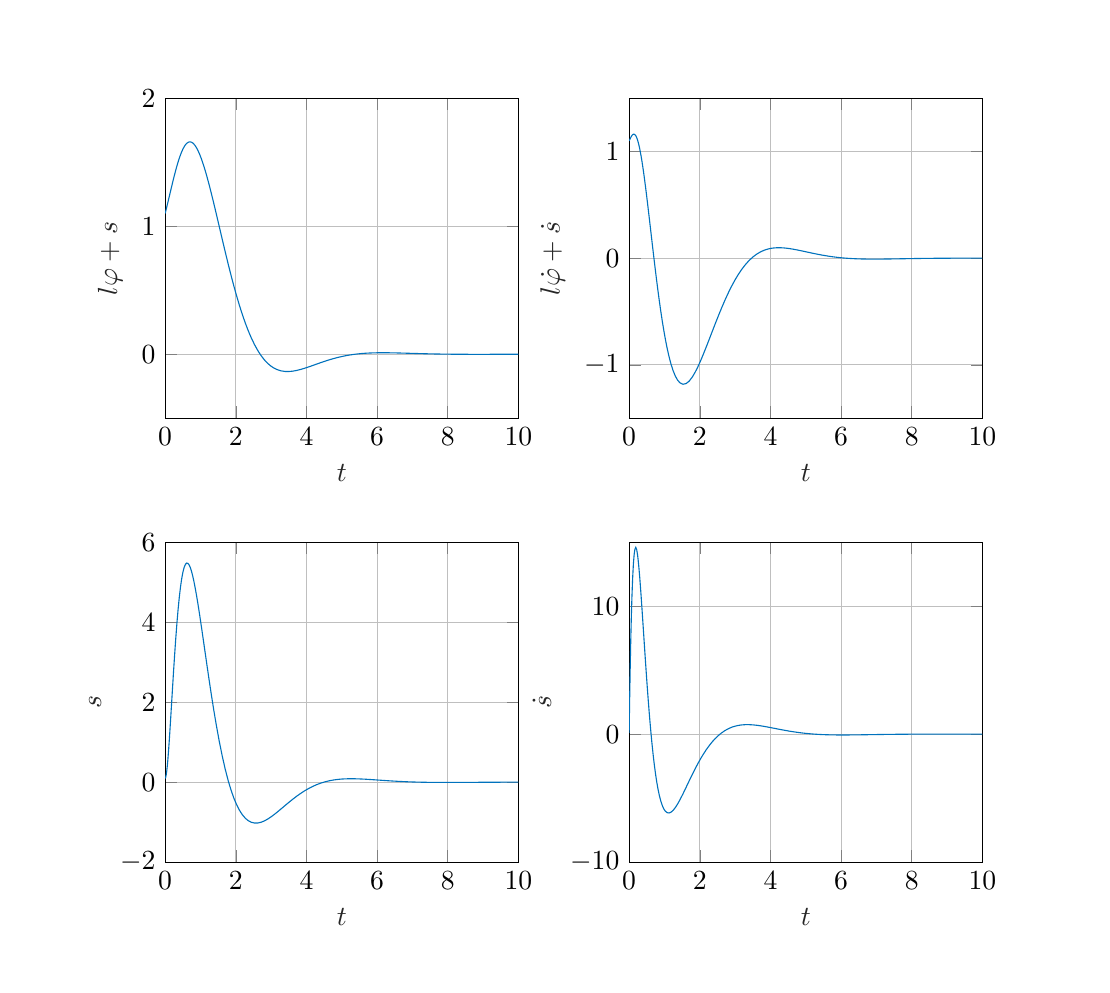
\begin{tikzpicture}

\begin{axis}[%
width=0.37\linewidth,
height=0.335\linewidth,
at={(0\linewidth,0.465\linewidth)},
scale only axis,
xmin=0,
xmax=10,
xlabel style={font=\color{white!15!black}},
xlabel={$t$},
ymin=-0.5,
ymax=2,
ylabel style={font=\color{white!15!black}},
ylabel={$l\varphi+s$},
axis background/.style={fill=white},
xmajorgrids,
ymajorgrids
]
\addplot [color=mycolor1, forget plot]
  table[row sep=crcr]{%
0	1.1\\
2.54858607093099e-05	1.10002803469036\\
5.09717214186197e-05	1.10005606986787\\
7.64575821279296e-05	1.10008410553256\\
0.000101943442837239	1.10011214168443\\
0.000229372746383789	1.10025232975196\\
0.000356802049930338	1.10039253000089\\
0.000484231353476887	1.10053274243268\\
0.000611660657023437	1.10067296704876\\
0.00124880717475618	1.1013742729406\\
0.00188595369248893	1.10207588363096\\
0.00252310021022168	1.10277779925453\\
0.00316024672795442	1.10348001992229\\
0.00634597931661816	1.10699570133106\\
0.00953171190528189	1.11051901191795\\
0.0127174444939456	1.11404993943971\\
0.0159031770826094	1.11758845818931\\
0.0313360088879608	1.13483664709144\\
0.0467688406933122	1.1522526617583\\
0.0622016724986636	1.16982131950304\\
0.0776345043040151	1.18752356190043\\
0.0984414507563126	1.21156061777887\\
0.11924839720861	1.23572571782794\\
0.140055343660908	1.25993898720323\\
0.160862290113205	1.28411896720477\\
0.187797275331352	1.31523299188692\\
0.214732260549498	1.34594507488482\\
0.241667245767645	1.3760548218798\\
0.268602230985791	1.40537770231811\\
0.3012913364769	1.43965545712635\\
0.33398044196801	1.47219611357368\\
0.366669547459119	1.50271572895312\\
0.399358652950228	1.53097775874453\\
0.434192889267375	1.55838010168498\\
0.469027125584522	1.58276169113904\\
0.50386136190167	1.60394790591079\\
0.538695598218817	1.62181263800103\\
0.574195026583334	1.63651069839402\\
0.609694454947852	1.64760951500695\\
0.645193883312369	1.65508947087615\\
0.680693311676887	1.65896375356063\\
0.713131566376002	1.65938710989633\\
0.745569821075117	1.65688841137829\\
0.778008075774232	1.65153667363538\\
0.810446330473348	1.6434131376296\\
0.851897583929155	1.62914653074493\\
0.893348837384962	1.6107315830935\\
0.934800090840769	1.58841334279663\\
0.976251344296576	1.56244636376933\\
1.02722424063342	1.52590322151683\\
1.07819713697026	1.48477213205153\\
1.12917003330711	1.43958358188198\\
1.18014292964395	1.39085050206675\\
1.24455508426323	1.32497833133208\\
1.3089672388825	1.25527625538121\\
1.37337939350178	1.18271276004426\\
1.43779154812105	1.10816205559932\\
1.52500437861299	1.00547669651352\\
1.61221720910493	0.902518458694745\\
1.69943003959687	0.800923947447121\\
1.78664287008881	0.702007880099372\\
1.86598176811546	0.61527164079401\\
1.94532066614212	0.53237855264519\\
2.02465956416877	0.453877744872282\\
2.10399846219542	0.380186222160292\\
2.18690094226423	0.308648028347369\\
2.26980342233303	0.242900436516363\\
2.35270590240184	0.183044381553622\\
2.43560838247064	0.129093670960467\\
2.52985757900805	0.0748433482856214\\
2.62410677554547	0.0278926393242984\\
2.71835597208288	-0.0120880726670246\\
2.81260516862029	-0.0454780884364472\\
2.90072951064794	-0.0711215896629935\\
2.98885385267559	-0.0917994862423477\\
3.07697819470325	-0.107935356666963\\
3.1651025367309	-0.119947668181357\\
3.27819004724366	-0.129987389865662\\
3.39127755775642	-0.134837990831636\\
3.50436506826919	-0.135369521728798\\
3.61745257878195	-0.132362817077161\\
3.72793394733698	-0.126700300308388\\
3.838415315892	-0.119001191968422\\
3.94889668444703	-0.10983531852419\\
4.05937805300206	-0.0996884789529299\\
4.17436803791206	-0.0885368569941304\\
4.28935802282206	-0.0771925588239616\\
4.40434800773206	-0.0659926294045985\\
4.51933799264206	-0.0552013406393688\\
4.63970840401057	-0.0445641839046601\\
4.76007881537908	-0.0347682104796731\\
4.88044922674758	-0.0259248213402803\\
5.00081963811609	-0.018099634320028\\
5.11120998050479	-0.0118393862132657\\
5.22160032289348	-0.00644358887472087\\
5.33199066528217	-0.00188212745049906\\
5.44238100767086	0.00188541067066781\\
5.55036137756258	0.00485222760497682\\
5.6583417474543	0.00717106686012769\\
5.76632211734602	0.00890646316156121\\
5.87430248723774	0.0101214718964828\\
5.98541521135754	0.0108952795168185\\
6.09652793547733	0.0112582322582771\\
6.20764065959713	0.0112787535354834\\
6.31875338371693	0.0110183967578253\\
6.42839314776138	0.0105416983750043\\
6.53803291180582	0.00989966191457675\\
6.64767267585027	0.00913850922233356\\
6.75731243989472	0.00829770029434024\\
6.87252887972755	0.00736560285794915\\
6.98774531956038	0.00641790390388311\\
7.10296175939322	0.00548276423263143\\
7.21817819922605	0.00458223976926805\\
7.33844778868161	0.00369749529548409\\
7.45871737813718	0.00288301247270255\\
7.57898696759274	0.00214796190436192\\
7.6992565570483	0.00149772696118024\\
7.80974608203009	0.000976825758853149\\
7.92023560701188	0.000528092154930896\\
8.03072513199367	0.00014897725009897\\
8.14121465697546	-0.000163921532615068\\
8.24899723099146	-0.000409499104686645\\
8.35677980500746	-0.000601363961526773\\
8.46456237902346	-0.00074487242427027\\
8.57234495303946	-0.000845256085906256\\
8.68736414265868	-0.000910730332814258\\
8.80238333227791	-0.000939820888346578\\
8.91740252189713	-0.000938842485677246\\
9.03242171151635	-0.000913429623561664\\
9.14839112186665	-0.000868325358320247\\
9.26436053221695	-0.000808764457905927\\
9.38032994256725	-0.000739182089465509\\
9.49629935291755	-0.00066329818750528\\
9.62222451468816	-0.000577441794585499\\
9.74814967645877	-0.000491387615454166\\
9.87407483822939	-0.00040788387093939\\
10	-0.000328982573063778\\
};
\end{axis}

\begin{axis}[%
width=0.37\linewidth,
height=0.335\linewidth,
at={(0.486\linewidth,0.465\linewidth)},
scale only axis,
xmin=0,
xmax=10,
xlabel style={font=\color{white!15!black}},
xlabel={$t$},
ymin=-1.5,
ymax=1.5,
ylabel style={font=\color{white!15!black}},
ylabel={$l\dot\varphi+\dot s$},
axis background/.style={fill=white},
xmajorgrids,
ymajorgrids
]
\addplot [color=mycolor1, forget plot]
  table[row sep=crcr]{%
0	1.1\\
2.54858607093099e-05	1.1000191146387\\
5.09717214186197e-05	1.10003822976211\\
7.64575821279296e-05	1.10005734536779\\
0.000101943442837239	1.1000764614533\\
0.000229372746383789	1.10017204899318\\
0.000356802049930338	1.10026764816379\\
0.000484231353476887	1.10036325866123\\
0.000611660657023437	1.10045888018195\\
0.00124880717475618	1.10093714253556\\
0.00188595369248893	1.10141563514752\\
0.00252310021022168	1.10189432048179\\
0.00316024672795442	1.10237316122671\\
0.00634597931661816	1.104768404779\\
0.00953171190528189	1.10716206544388\\
0.0127174444939456	1.10954972809524\\
0.0159031770826094	1.11192710937323\\
0.0313360088879608	1.12316511211538\\
0.0467688406933122	1.13364116843141\\
0.0622016724986636	1.14299188393029\\
0.0776345043040151	1.15090433205775\\
0.0984414507563126	1.15883705422626\\
0.11924839720861	1.16321121026034\\
0.140055343660908	1.16368057783604\\
0.160862290113205	1.15998695465256\\
0.187797275331352	1.14876248022037\\
0.214732260549498	1.13024964445992\\
0.241667245767645	1.10456796294008\\
0.268602230985791	1.0719108506201\\
0.3012913364769	1.02334809689795\\
0.33398044196801	0.965865876779245\\
0.366669547459119	0.900438345308326\\
0.399358652950228	0.82798956912763\\
0.434192889267375	0.744143696440853\\
0.469027125584522	0.654768005640479\\
0.50386136190167	0.561117973026402\\
0.538695598218817	0.464315706585596\\
0.574195026583334	0.363518185323761\\
0.609694454947852	0.261674784370942\\
0.645193883312369	0.159782089889563\\
0.680693311676887	0.0587063840691038\\
0.713131566376002	-0.0322824790530225\\
0.745569821075117	-0.121400608261017\\
0.778008075774232	-0.208181879345116\\
0.810446330473348	-0.292225909537456\\
0.851897583929155	-0.395097474634495\\
0.893348837384962	-0.492358251653431\\
0.934800090840769	-0.583556024426793\\
0.976251344296576	-0.668354231281369\\
1.02722424063342	-0.763516540242756\\
1.07819713697026	-0.848442301711684\\
1.12917003330711	-0.923096221207504\\
1.18014292964395	-0.987559273626459\\
1.24455508426323	-1.05474811918224\\
1.3089672388825	-1.10672450556202\\
1.37337939350178	-1.14439081226497\\
1.43779154812105	-1.16866878473231\\
1.52500437861299	-1.18194689722753\\
1.61221720910493	-1.17548743239906\\
1.69943003959687	-1.15223659583413\\
1.78664287008881	-1.11473366629324\\
1.86598176811546	-1.07029982474639\\
1.94532066614212	-1.01810440721825\\
2.02465956416877	-0.959885516980571\\
2.10399846219542	-0.897175427487553\\
2.18690094226423	-0.82835594178248\\
2.26980342233303	-0.757628720579591\\
2.35270590240184	-0.68626920857663\\
2.43560838247064	-0.615364193107812\\
2.52985757900805	-0.536480914113029\\
2.62410677554547	-0.460523667315011\\
2.71835597208288	-0.388394025208122\\
2.81260516862029	-0.320782811451508\\
2.90072951064794	-0.262097862312008\\
2.98885385267559	-0.208066084432487\\
3.07697819470325	-0.158839564293527\\
3.1651025367309	-0.114483048572875\\
3.27819004724366	-0.0646654322266648\\
3.39127755775642	-0.0225709766715486\\
3.50436506826919	0.0122033997712124\\
3.61745257878195	0.0401268739978291\\
3.72793394733698	0.0613178575586139\\
3.838415315892	0.077117179329432\\
3.94889668444703	0.0881487440503531\\
4.05937805300206	0.0950060327099684\\
4.17436803791206	0.0983360287791075\\
4.28935802282206	0.0984527186661006\\
4.40434800773206	0.0959784477318334\\
4.51933799264206	0.0914607570099576\\
4.63970840401057	0.085080066965739\\
4.76007881537908	0.0775364725468247\\
4.88044922674758	0.0692839249052187\\
5.00081963811609	0.0606931475270544\\
5.11120998050479	0.0527800123130275\\
5.22160032289348	0.0450420157908229\\
5.33199066528217	0.0376352668426881\\
5.44238100767086	0.0306786056291139\\
5.55036137756258	0.0243923863680228\\
5.6583417474543	0.0186722916368811\\
5.76632211734602	0.0135483728176707\\
5.87430248723774	0.00903371215052091\\
5.98541521135754	0.0050209624887797\\
6.09652793547733	0.00162745664666096\\
6.20764065959713	-0.001179570292021\\
6.31875338371693	-0.00343790962103019\\
6.42839314776138	-0.00517130421123037\\
6.53803291180582	-0.00646388509338802\\
6.64767267585027	-0.00736650094289767\\
6.75731243989472	-0.00792754511880915\\
6.87252887972755	-0.00820098028988855\\
6.98774531956038	-0.00820635748564752\\
7.10296175939322	-0.00799580551052042\\
7.21817819922605	-0.00761515548060165\\
7.33844778868161	-0.00708109248679452\\
7.45871737813718	-0.00645108078948063\\
7.57898696759274	-0.00576274926603753\\
7.6992565570483	-0.00504682426059642\\
7.80974608203009	-0.00438663008130702\\
7.92023560701188	-0.00374137265667837\\
8.03072513199367	-0.00312403224818784\\
8.14121465697546	-0.0025444795191224\\
8.24899723099146	-0.00202239353407259\\
8.35677980500746	-0.00154741377797626\\
8.46456237902346	-0.00112199378891954\\
8.57234495303946	-0.000747188904243047\\
8.68736414265868	-0.000402745456740269\\
8.80238333227791	-0.000113489737418945\\
8.91740252189713	0.000123680860366697\\
9.03242171151635	0.000312312965431984\\
9.14839112186665	0.000457520410821186\\
9.26436053221695	0.000562617056662795\\
9.38032994256725	0.000632652618206467\\
9.49629935291755	0.000672362638354133\\
9.62222451468816	0.000686479763648518\\
9.74814967645877	0.000676317825788785\\
9.87407483822939	0.000647351575298634\\
10	0.000604248759183442\\
};
\end{axis}

\begin{axis}[%
width=0.37\linewidth,
height=0.335\linewidth,
at={(0\linewidth,0\linewidth)},
scale only axis,
xmin=0,
xmax=10,
xlabel style={font=\color{white!15!black}},
xlabel={$t$},
ymin=-2,
ymax=6,
ylabel style={font=\color{white!15!black}},
ylabel={$s$},
axis background/.style={fill=white},
xmajorgrids,
ymajorgrids
]
\addplot [color=mycolor1, forget plot]
  table[row sep=crcr]{%
0	0.1\\
2.54858607093099e-05	0.100002612598576\\
5.09717214186197e-05	0.100005353201835\\
7.64575821279296e-05	0.100008221779289\\
0.000101943442837239	0.100011218300454\\
0.000229372746383789	0.100028118995352\\
0.000356802049930338	0.100048213713238\\
0.000484231353476887	0.100071498649027\\
0.000611660657023437	0.100097970000606\\
0.00124880717475618	0.100277990126945\\
0.00188595369248893	0.100537102037752\\
0.00252310021022168	0.100874833802184\\
0.00316024672795442	0.101290715327787\\
0.00634597931661816	0.104526037432046\\
0.00953171190528189	0.109645643840348\\
0.0127174444939456	0.116592817207857\\
0.0159031770826094	0.125311933506208\\
0.0313360088879608	0.190885505798938\\
0.0467688406933122	0.290968937198064\\
0.0622016724986636	0.420274830711786\\
0.0776345043040151	0.573972517904963\\
0.0984414507563126	0.812122118910261\\
0.11924839720861	1.07743601434923\\
0.140055343660908	1.36186186694595\\
0.160862290113205	1.65830047780504\\
0.187797275331352	2.04998568828578\\
0.214732260549498	2.44126821598341\\
0.241667245767645	2.82378591714349\\
0.268602230985791	3.1905098604791\\
0.3012913364769	3.60652260288753\\
0.33398044196801	3.98540799487201\\
0.366669547459119	4.32327633948865\\
0.399358652950228	4.61718022223278\\
0.434192889267375	4.88038488658135\\
0.469027125584522	5.09314843768684\\
0.50386136190167	5.25719220790804\\
0.538695598218817	5.37435419105481\\
0.574195026583334	5.44806057332036\\
0.609694454947852	5.4794922371462\\
0.645193883312369	5.4724148844414\\
0.680693311676887	5.43033065079112\\
0.713131566376002	5.36426853320826\\
0.745569821075117	5.27488825911101\\
0.778008075774232	5.16491578875281\\
0.810446330473348	5.03687084983152\\
0.851897583929155	4.85071738283321\\
0.893348837384962	4.64377722252054\\
0.934800090840769	4.42042716917663\\
0.976251344296576	4.18448690531777\\
1.02722424063342	3.88212453695898\\
1.07819713697026	3.57168085248942\\
1.12917003330711	3.25803791450391\\
1.18014292964395	2.94523677731748\\
1.24455508426323	2.55643453839775\\
1.3089672388825	2.17982265211905\\
1.37337939350178	1.81949046320177\\
1.43779154812105	1.47860757003637\\
1.52500437861299	1.05227080859453\\
1.61221720910493	0.668429731812091\\
1.69943003959687	0.327861688092297\\
1.78664287008881	0.0310931192857646\\
1.86598176811546	-0.20131362900822\\
1.94532066614212	-0.399962051564149\\
2.02465956416877	-0.566798958602478\\
2.10399846219542	-0.703710670136387\\
2.18690094226423	-0.817046730879368\\
2.26980342233303	-0.902832814481342\\
2.35270590240184	-0.963812394259307\\
2.43560838247064	-1.00255995451201\\
2.52985757900805	-1.02281066837662\\
2.62410677554547	-1.02141585213068\\
2.71835597208288	-1.00191439575284\\
2.81260516862029	-0.967493548608701\\
2.90072951064794	-0.924424625125867\\
2.98885385267559	-0.873197977803757\\
3.07697819470325	-0.815862521382532\\
3.1651025367309	-0.754229718168345\\
3.27819004724366	-0.671395171806299\\
3.39127755775642	-0.587076815750994\\
3.50436506826919	-0.503716042675915\\
3.61745257878195	-0.423240080885648\\
3.72793394733698	-0.348838266089491\\
3.838415315892	-0.279656839430231\\
3.94889668444703	-0.216409129349342\\
4.05937805300206	-0.159552227953218\\
4.17436803791206	-0.107402447822189\\
4.28935802282206	-0.0623897754119365\\
4.40434800773206	-0.0243135911484665\\
4.51933799264206	0.00712974583234607\\
4.63970840401057	0.0333870240021995\\
4.76007881537908	0.053470013938627\\
4.88044922674758	0.0680551010421962\\
5.00081963811609	0.0777946370279879\\
5.11120998050479	0.0830295811742997\\
5.22160032289348	0.085286761826193\\
5.33199066528217	0.0850685482692883\\
5.44238100767086	0.0828263214411293\\
5.55036137756258	0.07907480263898\\
5.6583417474543	0.0741598346285095\\
5.76632211734602	0.0684097023711717\\
5.87430248723774	0.0621051566359053\\
5.98541521135754	0.0552945899798284\\
6.09652793547733	0.0483859912950292\\
6.20764065959713	0.0415686054327921\\
6.31875338371693	0.0349922393255431\\
6.42839314776138	0.0288529849046201\\
6.53803291180582	0.0231451750244927\\
6.64767267585027	0.0179260820432118\\
6.75731243989472	0.0132323531336755\\
6.87252887972755	0.00888551338899655\\
6.98774531956038	0.00513591814636171\\
7.10296175939322	0.00196648668592221\\
7.21817819922605	-0.000648454060620243\\
7.33844778868161	-0.00282416723734958\\
7.45871737813718	-0.00448707334284123\\
7.57898696759274	-0.00569348980944574\\
7.6992565570483	-0.00649770251029344\\
7.80974608203009	-0.00692896532716657\\
7.92023560701188	-0.00711240867928468\\
8.03072513199367	-0.00708998091434449\\
8.14121465697546	-0.00689935421001832\\
8.24899723099146	-0.00658453313355076\\
8.35677980500746	-0.00617370923834054\\
8.46456237902346	-0.00569402984991208\\
8.57234495303946	-0.00516871445259074\\
8.68736414265868	-0.00458037931988717\\
8.80238333227791	-0.00398422281750386\\
8.91740252189713	-0.00339751661580115\\
9.03242171151635	-0.00283375931696344\\
9.14839112186665	-0.00229908352059699\\
9.26436053221695	-0.00180598388849689\\
9.38032994256725	-0.00135953671201561\\
9.49629935291755	-0.000962770500473512\\
9.62222451468816	-0.000589581684245157\\
9.74814967645877	-0.000275279084679243\\
9.87407483822939	-1.72435412995904e-05\\
10	0.000187905748564992\\
};
\end{axis}

\begin{axis}[%
width=0.37\linewidth,
height=0.335\linewidth,
at={(0.486\linewidth,0\linewidth)},
scale only axis,
xmin=0,
xmax=10,
xlabel style={font=\color{white!15!black}},
xlabel={$t$},
ymin=-10,
ymax=15,
ylabel style={font=\color{white!15!black}},
ylabel={$\dot s$},
axis background/.style={fill=white},
xmajorgrids,
ymajorgrids
]
\addplot [color=mycolor1, forget plot]
  table[row sep=crcr]{%
0	0.1\\
2.54858607093099e-05	0.105023174613241\\
5.09717214186197e-05	0.110045152851505\\
7.64575821279296e-05	0.115065934901646\\
0.000101943442837239	0.120085520950492\\
0.000229372746383789	0.145165517712687\\
0.000356802049930338	0.17021564245331\\
0.000484231353476887	0.195235918499377\\
0.000611660657023437	0.220226369163116\\
0.00124880717475618	0.344732056649361\\
0.00188595369248893	0.468495597911356\\
0.00252310021022168	0.59151989037251\\
0.00316024672795442	0.713807822288535\\
0.00634597931661816	1.31430255216107\\
0.00953171190528189	1.89681624791384\\
0.0127174444939456	2.46169973039429\\
0.0159031770826094	3.00929832724066\\
0.0313360088879608	5.42827080689074\\
0.0467688406933122	7.4861752832632\\
0.0622016724986636	9.21703186660089\\
0.0776345043040151	10.6524548076364\\
0.0984414507563126	12.1714316200069\\
0.11924839720861	13.2704436039783\\
0.140055343660908	14.007080298577\\
0.160862290113205	14.4334910286877\\
0.187797275331352	14.6003762526161\\
0.214732260549498	14.4106663656252\\
0.241667245767645	13.9380365667242\\
0.268602230985791	13.2473579456131\\
0.3012913364769	12.1954343026302\\
0.33398044196801	10.9794569918122\\
0.366669547459119	9.66166269108348\\
0.399358652950228	8.2955696352685\\
0.434192889267375	6.83430472486027\\
0.469027125584522	5.3995000815915\\
0.50386136190167	4.01712045233212\\
0.538695598218817	2.70891311399718\\
0.574195026583334	1.46783433021718\\
0.609694454947852	0.325806363685244\\
0.645193883312369	-0.713483883161669\\
0.680693311676887	-1.64752475941452\\
0.713131566376002	-2.40909627666503\\
0.745569821075117	-3.08628767516325\\
0.778008075774232	-3.68260259373215\\
0.810446330473348	-4.20160774287314\\
0.851897583929155	-4.75862559994265\\
0.893348837384962	-5.20662674471887\\
0.934800090840769	-5.55615671443183\\
0.976251344296576	-5.81650495345503\\
1.02722424063342	-6.02766781625173\\
1.07819713697026	-6.13595416839243\\
1.12917003330711	-6.15762329912059\\
1.18014292964395	-6.10605818227451\\
1.24455508426323	-5.95481822568867\\
1.3089672388825	-5.72937192476504\\
1.37337939350178	-5.44889651645905\\
1.43779154812105	-5.12840551643738\\
1.52500437861299	-4.6534444381045\\
1.61221720910493	-4.15387534222525\\
1.69943003959687	-3.64797478446812\\
1.78664287008881	-3.15040889994482\\
1.86598176811546	-2.71438823449423\\
1.94532066614212	-2.29924026416062\\
2.02465956416877	-1.90837017219133\\
2.10399846219542	-1.54480043983508\\
2.18690094226423	-1.19621056532048\\
2.26980342233303	-0.879810128246576\\
2.35270590240184	-0.595518414264977\\
2.43560838247064	-0.34314371107869\\
2.52985757900805	-0.0941281337548297\\
2.62410677554547	0.116797792001143\\
2.71835597208288	0.292054832999637\\
2.81260516862029	0.43401999940763\\
2.90072951064794	0.538952098743786\\
2.98885385267559	0.619597002654289\\
3.07697819470325	0.678370474598316\\
3.1651025367309	0.717588551533336\\
3.27819004724366	0.742874640859925\\
3.39127755775642	0.744517487184721\\
3.50436506826919	0.727012852170041\\
3.61745257878195	0.694326786832583\\
3.72793394733698	0.651181320795378\\
3.838415315892	0.600152518401419\\
3.94889668444703	0.543965066553469\\
4.05937805300206	0.484907028241272\\
4.17436803791206	0.422470609719535\\
4.28935802282206	0.360875202153003\\
4.40434800773206	0.301583387421946\\
4.51933799264206	0.245707330995002\\
4.63970840401057	0.191760933103982\\
4.76007881537908	0.143059325558514\\
4.88044922674758	0.0999402351688239\\
5.00081963811609	0.0625419693397694\\
5.11120998050479	0.0332335512899456\\
5.22160032289348	0.00851074696407778\\
5.33199066528217	-0.0118813992889597\\
5.44238100767086	-0.0282318196578923\\
5.55036137756258	-0.0406329784502001\\
5.6583417474543	-0.0498520630310575\\
5.76632211734602	-0.0562567197210785\\
5.87430248723774	-0.0601966120252344\\
5.98541521135754	-0.0620382077406752\\
6.09652793547733	-0.0620149576103604\\
6.20764065959713	-0.0604787297734713\\
6.31875338371693	-0.0577411823546904\\
6.42839314776138	-0.0541383976146293\\
6.53803291180582	-0.0498976175186703\\
6.64767267585027	-0.0452396846782009\\
6.75731243989472	-0.040350209471988\\
6.87252887972755	-0.0351344312422226\\
6.98774531956038	-0.0299913682372169\\
7.10296175939322	-0.0250431564704654\\
7.21817819922605	-0.0203825180637967\\
7.33844778868161	-0.0158975060162108\\
7.45871737813718	-0.0118498777089269\\
7.57898696759274	-0.00826728501730038\\
7.6992565570483	-0.00516089081219485\\
7.80974608203009	-0.00272323651704141\\
7.92023560701188	-0.0006682210713509\\
8.03072513199367	0.00102559814158193\\
8.14121465697546	0.00238246860063153\\
8.24899723099146	0.00340794700518984\\
8.35677980500746	0.00416975902649836\\
8.46456237902346	0.0046983950742267\\
8.57234495303946	0.00502284844188913\\
8.68736414265868	0.00517578834228557\\
8.80238333227791	0.00516379021681295\\
8.91740252189713	0.00501928142127515\\
9.03242171151635	0.00477073940621837\\
9.14839112186665	0.0044408869880831\\
9.26436053221695	0.00405617027014128\\
9.38032994256725	0.00363767984446751\\
9.49629935291755	0.00320281158929586\\
9.62222451468816	0.00272887809921616\\
9.74814967645877	0.00226812199546839\\
9.87407483822939	0.00183223514130911\\
10	0.00142960712019944\\
};
\end{axis}

\begin{axis}[%
width=1.104\linewidth,
height=0.982\linewidth,
at={(-0.144\linewidth,-0.108\linewidth)},
scale only axis,
xmin=0,
xmax=1,
ymin=0,
ymax=1,
axis line style={draw=none},
ticks=none,
axis x line*=bottom,
axis y line*=left
]
\end{axis}
\end{tikzpicture}%
	\caption{Поведение линеаризированной системы при действии линейного стабилизатора с полной обратной связью для заданных собственных значений замкнутой системы $\mu_1 = -2 + i$, $\mu_2 = -2 - i$, $\mu_3 = \mu_4 = -3$ из положения $z^0 = [1,\!1,\,1,\!1,\,0,\!1,\,0,\!1]$.}
\end{figure}

\begin{figure}[t]
	\centering
	% This file was created by matlab2tikz.
%
%The latest updates can be retrieved from
%  http://www.mathworks.com/matlabcentral/fileexchange/22022-matlab2tikz-matlab2tikz
%where you can also make suggestions and rate matlab2tikz.
%
\definecolor{mycolor1}{rgb}{0.00000,0.44700,0.74100}%
%
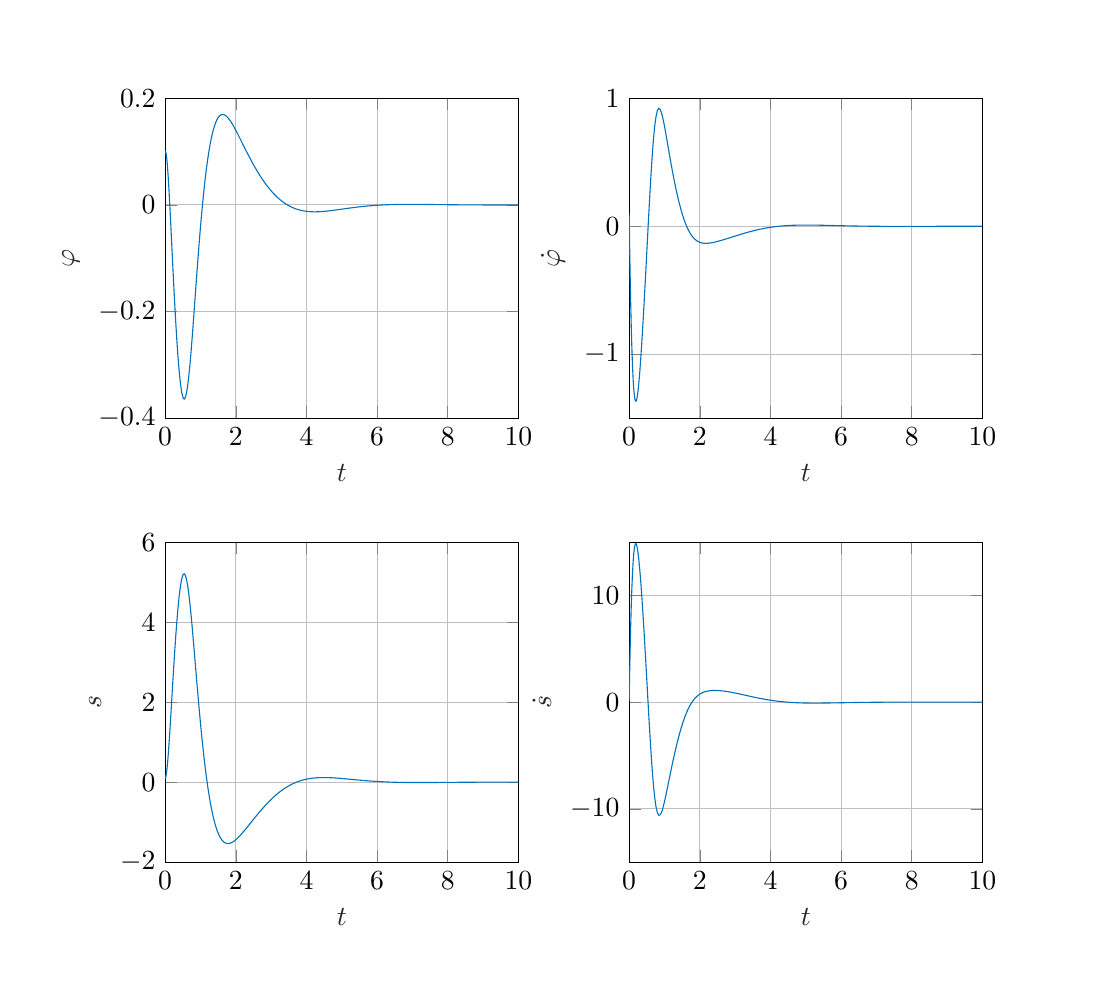
\begin{tikzpicture}

\begin{axis}[%
width=0.37\linewidth,
height=0.335\linewidth,
at={(0\linewidth,0.465\linewidth)},
scale only axis,
xmin=0,
xmax=10,
xlabel style={font=\color{white!15!black}},
xlabel={$t$},
ymin=-0.4,
ymax=0.2,
ylabel style={font=\color{white!15!black}},
ylabel={$\varphi$},
axis background/.style={fill=white},
xmajorgrids,
ymajorgrids
]
\addplot [color=mycolor1, forget plot]
  table[row sep=crcr]{%
0	0.1\\
2.54858607093099e-05	0.100002542241081\\
5.09717214186197e-05	0.100005071794116\\
7.64575821279296e-05	0.100007588662007\\
0.000101943442837239	0.100010092847652\\
0.000229372746383789	0.100022423643682\\
0.000356802049930338	0.10003443781837\\
0.000484231353476887	0.100046135733744\\
0.000611660657023437	0.100057517751561\\
0.00124880717475618	0.100109702019833\\
0.00188595369248893	0.100154042954593\\
0.00252310021022168	0.100190585467292\\
0.00316024672795442	0.10021937430031\\
0.00634597931661816	0.100248568501999\\
0.00953171190528189	0.100090535390792\\
0.0127174444939456	0.0997506813639295\\
0.0159031770826094	0.0992343154801516\\
0.030492828041498	0.094759958827207\\
0.0450824790003867	0.0871646131411665\\
0.0596721299592754	0.0768842324129727\\
0.074261780918164	0.0643245306109301\\
0.0941432516409177	0.0442090466006986\\
0.114024722363671	0.0213823270549922\\
0.133906193086425	-0.00342171098468544\\
0.153787663809179	-0.0295529516658565\\
0.176775172097389	-0.0606851736341787\\
0.1997626803856	-0.0921379844124597\\
0.22275018867381	-0.12332290022964\\
0.245737696962021	-0.153736091730594\\
0.274026916165467	-0.189500744681148\\
0.302316135368912	-0.222903977225067\\
0.330605354572358	-0.253478885013586\\
0.358894573775803	-0.280829343327749\\
0.396486146251279	-0.311670550233278\\
0.434077718726756	-0.335720261895254\\
0.471669291202232	-0.352555627732742\\
0.509260863677708	-0.36193862214873\\
0.540213688475597	-0.364032625283505\\
0.571166513273486	-0.361085819615587\\
0.602119338071374	-0.353262947325877\\
0.633072162869263	-0.340883952771678\\
0.664024987667151	-0.324383072081017\\
0.69497781246504	-0.304282221272703\\
0.725930637262928	-0.281187740848446\\
0.756883462060817	-0.25575727087786\\
0.797053481137648	-0.220342285870515\\
0.837223500214478	-0.183545418868588\\
0.877393519291309	-0.146622519183045\\
0.91756353836814	-0.110479221370379\\
0.952370420602463	-0.0803372275885285\\
0.987177302836788	-0.0516660234644023\\
1.02198418507111	-0.0246787345156981\\
1.05679106730544	0.000459683971870586\\
1.09368066159204	0.0249786274297596\\
1.13057025587864	0.047316449457227\\
1.16745985016524	0.0674995436524582\\
1.20434944445184	0.0855581346357198\\
1.24474654914447	0.102963432152663\\
1.28514365383711	0.118014251403039\\
1.32554075852974	0.130836731804682\\
1.36593786322237	0.141557525405269\\
1.42093493347181	0.153013413435409\\
1.47593200372126	0.161190894889823\\
1.5309290739707	0.166459496400223\\
1.58592614422014	0.16917209994094\\
1.63359099546143	0.169721117084675\\
1.68125584670273	0.168838113179526\\
1.72892069794402	0.166736051094692\\
1.77658554918532	0.163605228231887\\
1.82425040042662	0.159620767762875\\
1.87191525166791	0.154950548441066\\
1.91958010290921	0.149740703268416\\
1.9672449541505	0.144115633684731\\
2.0158661806718	0.138062532879443\\
2.06448740719309	0.131790089626424\\
2.11310863371438	0.125380551218801\\
2.16172986023568	0.11890392903546\\
2.22302720160279	0.11073520873055\\
2.2843245429699	0.10263615405362\\
2.34562188433701	0.0946696428592774\\
2.40691922570412	0.0868956739754753\\
2.46821656707124	0.0793610242311741\\
2.52951390843835	0.0720850229493673\\
2.59081124980546	0.0650862304076006\\
2.65210859117257	0.0583857295214626\\
2.71987480973792	0.0513444334070927\\
2.78764102830327	0.044692078621331\\
2.85540724686862	0.0384342010817258\\
2.92317346543397	0.0325777351965039\\
3.00467164467537	0.0260702540557291\\
3.08616982391678	0.0201405649650518\\
3.16766800315818	0.0147800225565764\\
3.24916618239959	0.00997745538734826\\
3.36021379823374	0.00430092672589136\\
3.47126141406789	-0.000424735753137942\\
3.58230902990204	-0.00426146966573068\\
3.69335664573619	-0.00728298757595996\\
3.81651214351941	-0.00977523560244712\\
3.93966764130264	-0.0114702582031752\\
4.06282313908586	-0.0124804141517156\\
4.18597863686908	-0.0129136065309072\\
4.30211591848199	-0.0128853162068694\\
4.4182532000949	-0.0125181722087565\\
4.53439048170782	-0.0118887739304215\\
4.65052776332073	-0.0110630729471868\\
4.75570074672253	-0.0101948695326311\\
4.86087373012433	-0.00925396624638005\\
4.96604671352613	-0.00827429335232733\\
5.07121969692793	-0.00728414933976448\\
5.18692615251816	-0.00621077890684452\\
5.3026326081084	-0.00517873576466457\\
5.41833906369863	-0.00420745675253399\\
5.53404551928886	-0.00331112615408786\\
5.66728647117297	-0.00238422024258032\\
5.80052742305709	-0.0015764947564494\\
5.9337683749412	-0.000889524044249916\\
6.06700932682531	-0.000321307269065215\\
6.1992510839667	0.00013061657057446\\
6.33149284110808	0.00048042925260151\\
6.46373459824947	0.000738768225462785\\
6.59597635539086	0.000916079975500352\\
6.70422014522962	0.00100852517116915\\
6.81246393506837	0.00106068424728492\\
6.92070772490713	0.00107873357352898\\
7.02895151474588	0.00106829970687624\\
7.14272163893748	0.00103238367478147\\
7.25649176312907	0.000976734276671495\\
7.37026188732067	0.000906593098178115\\
7.48403201151226	0.000826426929482897\\
7.58491739379609	0.000750083036869898\\
7.68580277607991	0.00067134775581408\\
7.78668815836373	0.000592248623778827\\
7.88757354064755	0.000514457491322636\\
8.00803478682427	0.000425174301197768\\
8.12849603300099	0.000341485252312697\\
8.24895727917771	0.000264668473166158\\
8.36941852535443	0.000195567732809792\\
8.506412708598	0.000126953922568732\\
8.64340689184157	6.90091830370171e-05\\
8.78040107508514	2.14194744018333e-05\\
8.91739525832872	-1.63384647217668e-05\\
9.05752611823362	-4.55623933049746e-05\\
9.19765697813851	-6.64097806851041e-05\\
9.33778783804341	-8.00477039303801e-05\\
9.47791869794831	-8.75443916984885e-05\\
9.59090920757239	-8.98341583936207e-05\\
9.70389971719646	-8.94157061872193e-05\\
9.81689022682054	-8.68180892293349e-05\\
9.92988073644461	-8.25071881486869e-05\\
9.94741055233346	-8.17119938592992e-05\\
9.96494036822231	-8.08875548688592e-05\\
9.98247018411115	-8.00353511917024e-05\\
10	-7.91568341341078e-05\\
};
\end{axis}

\begin{axis}[%
width=0.37\linewidth,
height=0.335\linewidth,
at={(0.486\linewidth,0.465\linewidth)},
scale only axis,
xmin=0,
xmax=10,
xlabel style={font=\color{white!15!black}},
xlabel={$t$},
ymin=-1.5,
ymax=1,
ylabel style={font=\color{white!15!black}},
ylabel={$\dot\varphi$},
axis background/.style={fill=white},
xmajorgrids,
ymajorgrids
]
\addplot [color=mycolor1, forget plot]
  table[row sep=crcr]{%
0	0.1\\
2.54858607093099e-05	0.0995020966188931\\
5.09717214186197e-05	0.0990043070607769\\
7.64575821279296e-05	0.0985066313083259\\
0.000101943442837239	0.0980090693442184\\
0.000229372746383789	0.0955229657428433\\
0.000356802049930338	0.0930397042540171\\
0.000484231353476887	0.0905592827168533\\
0.000611660657023437	0.088081698972858\\
0.00124880717475618	0.0757362717667245\\
0.00188595369248893	0.0634614669870052\\
0.00252310021022168	0.0512570174864823\\
0.00316024672795442	0.0391226575705015\\
0.00634597931661816	-0.020507007792112\\
0.00953171190528189	-0.0784234669830529\\
0.0127174444939456	-0.134658383246773\\
0.0159031770826094	-0.189242644771718\\
0.030492828041498	-0.418972449837126\\
0.0450824790003867	-0.617405476375062\\
0.0596721299592754	-0.787038057449015\\
0.074261780918164	-0.930226802096536\\
0.0941432516409177	-1.08677437261434\\
0.114024722363671	-1.20362898801473\\
0.133906193086425	-1.2857721098876\\
0.153787663809179	-1.3378832675881\\
0.176775172097389	-1.36636312012691\\
0.1997626803856	-1.36629369157014\\
0.22275018867381	-1.34269290832421\\
0.245737696962021	-1.29986031777849\\
0.274026916165467	-1.2259555441592\\
0.302316135368912	-1.13321872901301\\
0.330605354572358	-1.02548985992727\\
0.358894573775803	-0.905782755161142\\
0.396486146251279	-0.732079081164572\\
0.434077718726756	-0.54534422636831\\
0.471669291202232	-0.349646344122817\\
0.509260863677708	-0.149599304184925\\
0.540213688475597	0.0148315991597242\\
0.571166513273486	0.175278288560251\\
0.602119338071374	0.327885668492374\\
0.633072162869263	0.468829811753716\\
0.664024987667151	0.594398500193934\\
0.69497781246504	0.701331314483335\\
0.725930637262928	0.787448202499041\\
0.756883462060817	0.851826179594303\\
0.797053481137648	0.903173534553218\\
0.837223500214478	0.922069935325402\\
0.877393519291309	0.914088164166631\\
0.91756353836814	0.884718832504805\\
0.952370420602463	0.846556370439094\\
0.987177302836788	0.800381840865793\\
1.02198418507111	0.748909708990284\\
1.05679106730544	0.694432800876479\\
1.09368066159204	0.635369883638856\\
1.13057025587864	0.576174118593449\\
1.16745985016524	0.517804370640125\\
1.20434944445184	0.461034401031534\\
1.24474654914447	0.401307337578568\\
1.28514365383711	0.344460670847918\\
1.32554075852974	0.290764593553759\\
1.36593786322237	0.240420589065559\\
1.42093493347181	0.177487871793529\\
1.47593200372126	0.121134927665648\\
1.5309290739707	0.0713831364428538\\
1.58592614422014	0.0281482397023302\\
1.63359099546143	-0.00419337992163318\\
1.68125584670273	-0.0320185679449802\\
1.72892069794402	-0.0556124828421961\\
1.77658554918532	-0.0752637857456524\\
1.82425040042662	-0.0912931472940196\\
1.87191525166791	-0.104108279791089\\
1.91958010290921	-0.114099039197869\\
1.9672449541505	-0.121612621925422\\
2.0158661806718	-0.127074043129632\\
2.06448740719309	-0.130671374829268\\
2.11310863371438	-0.132716451172803\\
2.16172986023568	-0.133478449389277\\
2.22302720160279	-0.13298636960781\\
2.2843245429699	-0.131210331165716\\
2.34562188433701	-0.128438896875998\\
2.40691922570412	-0.124938826139472\\
2.46821656707124	-0.12092494345449\\
2.52951390843835	-0.116495047858607\\
2.59081124980546	-0.111736506959683\\
2.65210859117257	-0.106753353642091\\
2.71987480973792	-0.101084116649688\\
2.78764102830327	-0.0952739270959724\\
2.85540724686862	-0.0893647739529788\\
2.92317346543397	-0.0834206052164563\\
3.00467164467537	-0.0763016320008866\\
3.08616982391678	-0.0692481773754801\\
3.16766800315818	-0.0623123370376303\\
3.24916618239959	-0.0555587244381867\\
3.36021379823374	-0.046737025027125\\
3.47126141406789	-0.038445317291022\\
3.58230902990204	-0.0307779265503565\\
3.69335664573619	-0.02378641343101\\
3.81651214351941	-0.0168546341111745\\
3.93966764130264	-0.0108277544228452\\
4.06282313908586	-0.0057093232913261\\
4.18597863686908	-0.00145802964013786\\
4.30211591848199	0.00180578318365389\\
4.4182532000949	0.00439254536815141\\
4.53439048170782	0.00636583762369125\\
4.65052776332073	0.00778845879044323\\
4.75570074672253	0.00865620516236564\\
4.86087373012433	0.0091793279437581\\
4.96604671352613	0.00940788690689238\\
5.07121969692793	0.00938791174091282\\
5.18692615251816	0.0091303977878162\\
5.3026326081084	0.00868020730158716\\
5.41833906369863	0.00808692305609329\\
5.53404551928886	0.00739320404910636\\
5.66728647117297	0.00651780104698261\\
5.80052742305709	0.00560743893290528\\
5.9337683749412	0.00470174415672418\\
6.06700932682531	0.00383065822831986\\
6.1992510839667	0.00302227729110248\\
6.33149284110808	0.0022855049423292\\
6.46373459824947	0.00162988033827314\\
6.59597635539086	0.0010604257176015\\
6.70422014522962	0.00065923357147057\\
6.81246393506837	0.000315144558219195\\
6.92070772490713	2.57551917821613e-05\\
7.02895151474588	-0.000211904972287692\\
7.14272163893748	-0.000409884189721627\\
7.25649176312907	-0.000559909120334954\\
7.37026188732067	-0.000667338176445847\\
7.48403201151226	-0.000737306328829472\\
7.58491739379609	-0.000772130849709291\\
7.68580277607991	-0.000785260338436508\\
7.78668815836373	-0.000780154079952985\\
7.88757354064755	-0.000759959164923311\\
8.00803478682427	-0.000720114510766569\\
8.12849603300099	-0.000667587811639073\\
8.24895727917771	-0.000606476103049439\\
8.36941852535443	-0.000540174176656329\\
8.506412708598	-0.000462083125357621\\
8.64340689184157	-0.00038456324198028\\
8.78040107508514	-0.000310351088375766\\
8.91739525832872	-0.000241388206707256\\
9.05752611823362	-0.000177662756058727\\
9.19765697813851	-0.000121674112623635\\
9.33778783804341	-7.37643259914985e-05\\
9.47791869794831	-3.39499390023519e-05\\
9.59090920757239	-7.54957717314858e-06\\
9.70389971719646	1.40825009817905e-05\\
9.81689022682054	3.13067322305284e-05\\
9.92988073644461	4.44996929050471e-05\\
9.94741055233346	4.62107309566151e-05\\
9.96494036822231	4.78365330641538e-05\\
9.98247018411115	4.93787246759062e-05\\
10	5.08389341747146e-05\\
};
\end{axis}

\begin{axis}[%
width=0.37\linewidth,
height=0.335\linewidth,
at={(0\linewidth,0\linewidth)},
scale only axis,
xmin=0,
xmax=10,
xlabel style={font=\color{white!15!black}},
xlabel={$t$},
ymin=-2,
ymax=6,
ylabel style={font=\color{white!15!black}},
ylabel={$s$},
axis background/.style={fill=white},
xmajorgrids,
ymajorgrids
]
\addplot [color=mycolor1, forget plot]
  table[row sep=crcr]{%
0	0.1\\
2.54858607093099e-05	0.100002612598807\\
5.09717214186197e-05	0.100005353203677\\
7.64575821279296e-05	0.100008221785505\\
0.000101943442837239	0.100011218315186\\
0.000229372746383789	0.100028119163072\\
0.000356802049930338	0.100048214344227\\
0.000484231353476887	0.100071500225464\\
0.000611660657023437	0.100097973176216\\
0.00124880717475618	0.100278017082813\\
0.00188595369248893	0.100537194644857\\
0.00252310021022168	0.100875054973367\\
0.00316024672795442	0.10129114879007\\
0.00634597931661816	0.104529498214155\\
0.00953171190528189	0.10965721539503\\
0.0127174444939456	0.116619922907318\\
0.0159031770826094	0.125364178193585\\
0.030492828041498	0.186704635751987\\
0.0450824790003867	0.279545744759442\\
0.0596721299592754	0.399478341216697\\
0.074261780918164	0.542395370404829\\
0.0941432516409177	0.767373831894828\\
0.114024722363671	1.01962410292125\\
0.133906193086425	1.2917147654667\\
0.153787663809179	1.57706627769797\\
0.176775172097389	1.91607625706864\\
0.1997626803856	2.25805537842606\\
0.22275018867381	2.59697038311502\\
0.245737696962021	2.92761312333564\\
0.274026916165467	3.31683114163393\\
0.302316135368912	3.68084311671468\\
0.330605354572358	4.01448108565467\\
0.358894573775803	4.31325988996543\\
0.396486146251279	4.65030301928909\\
0.434077718726756	4.91258504924381\\
0.471669291202232	5.09478139467301\\
0.509260863677708	5.19374057703005\\
0.540213688475597	5.2120452795036\\
0.571166513273486	5.17370709090903\\
0.602119338071374	5.08056642199367\\
0.633072162869263	4.93623618040869\\
0.664024987667151	4.74564307136379\\
0.69497781246504	4.51467111050165\\
0.725930637262928	4.25006712376454\\
0.756883462060817	3.9590693770463\\
0.797053481137648	3.55374967941269\\
0.837223500214478	3.13153256772398\\
0.877393519291309	2.70577932109453\\
0.91756353836814	2.28613284367433\\
0.952370420602463	1.93323421792542\\
0.987177302836788	1.59435921723247\\
1.02198418507111	1.27188196627289\\
1.05679106730544	0.967675075838756\\
1.09368066159204	0.666504614140417\\
1.13057025587864	0.387407315231195\\
1.16745985016524	0.130365249092551\\
1.20434944445184	-0.104695548482806\\
1.24474654914447	-0.337308045683001\\
1.28514365383711	-0.544988872788941\\
1.32554075852974	-0.728783183033608\\
1.36593786322237	-0.889773459944752\\
1.42093493347181	-1.07440870169666\\
1.47593200372126	-1.22238844120247\\
1.5309290739707	-1.3372244475987\\
1.58592614422014	-1.42234253450396\\
1.63359099546143	-1.47470659887693\\
1.68125584670273	-1.50962966891065\\
1.72892069794402	-1.52929015762967\\
1.77658554918532	-1.53565632053812\\
1.82425040042662	-1.53056094379403\\
1.87191525166791	-1.51578192127522\\
1.91958010290921	-1.49288574373969\\
1.9672449541505	-1.46322315769818\\
2.0158661806718	-1.42723465432631\\
2.06448740719309	-1.38657143019453\\
2.11310863371438	-1.34217909582326\\
2.16172986023568	-1.29487780624662\\
2.22302720160279	-1.2322029438871\\
2.2843245429699	-1.1670987001546\\
2.34562188433701	-1.10042957263722\\
2.40691922570412	-1.03301939361546\\
2.46821656707124	-0.965553377233059\\
2.52951390843835	-0.898441508148966\\
2.59081124980546	-0.83207538606562\\
2.65210859117257	-0.766861424858468\\
2.71987480973792	-0.696523015618102\\
2.78764102830327	-0.628308596405604\\
2.85540724686862	-0.562502420741732\\
2.92317346543397	-0.499387857620228\\
3.00467164467537	-0.427371876250335\\
3.08616982391678	-0.359834605739275\\
3.16766800315818	-0.296984891317733\\
3.24916618239959	-0.238977001611021\\
3.36021379823374	-0.167848383796321\\
3.47126141406789	-0.105822974934153\\
3.58230902990204	-0.0527202060145608\\
3.69335664573619	-0.0081582961238918\\
3.81651214351941	0.0318822692258189\\
3.93966764130264	0.0628474420070336\\
4.06282313908586	0.0856681945353902\\
4.18597863686908	0.101303782782918\\
4.30211591848199	0.110334248132001\\
4.4182532000949	0.114676933671466\\
4.53439048170782	0.115137495333202\\
4.65052776332073	0.112433561155743\\
4.75570074672253	0.107808986565559\\
4.86087373012433	0.101612937755565\\
4.96604671352613	0.0942643052045089\\
5.07121969692793	0.0861244906906004\\
5.18692615251816	0.0766301623133625\\
5.3026326081084	0.066926021413888\\
5.41833906369863	0.0573119876506841\\
5.53404551928886	0.0480243360531031\\
5.66728647117297	0.0379701900472653\\
5.80052742305709	0.0287899455483936\\
5.9337683749412	0.0206093077370494\\
6.06700932682531	0.0134965490285945\\
6.1992510839667	0.00751117160474331\\
6.33149284110808	0.00256301323595527\\
6.46373459824947	-0.00140777400269876\\
6.59597635539086	-0.00447219399501431\\
6.70422014522962	-0.00636586601669093\\
6.81246393506837	-0.00776844183703423\\
6.92070772490713	-0.00873718862541429\\
7.02895151474588	-0.00932649025182\\
7.14272163893748	-0.00959505195584163\\
7.25649176312907	-0.00956634496019879\\
7.37026188732067	-0.0092983859874707\\
7.48403201151226	-0.00884223078617196\\
7.58491739379609	-0.00831755012925802\\
7.68580277607991	-0.00771176424671555\\
7.78668815836373	-0.00705125055399623\\
7.88757354064755	-0.00635859523930095\\
8.00803478682427	-0.00551631165167119\\
8.12849603300099	-0.00468372283110971\\
8.24895727917771	-0.00388289598020456\\
8.36941852535443	-0.00313035697736294\\
8.506412708598	-0.00234833477283065\\
8.64340689184157	-0.0016550706436631\\
8.78040107508514	-0.00105576668106677\\
8.91739525832872	-0.00055165959940492\\
9.05752611823362	-0.00013211663341166\\
9.19765697813851	0.000197054568856002\\
9.33778783804341	0.000444415067870081\\
9.47791869794831	0.000618642377470501\\
9.59090920757239	0.000712272124783981\\
9.70389971719646	0.000770249957568529\\
9.81689022682054	0.000797919778087496\\
9.92988073644461	0.000800155342272088\\
9.94741055233346	0.000798516993799717\\
9.96494036822231	0.000796397882395139\\
9.98247018411115	0.000793814709014559\\
10	0.00079078394847688\\
};
\end{axis}

\begin{axis}[%
width=0.37\linewidth,
height=0.335\linewidth,
at={(0.486\linewidth,0\linewidth)},
scale only axis,
xmin=0,
xmax=10,
xlabel style={font=\color{white!15!black}},
xlabel={$t$},
ymin=-15,
ymax=15,
ylabel style={font=\color{white!15!black}},
ylabel={$\dot s$},
axis background/.style={fill=white},
xmajorgrids,
ymajorgrids
]
\addplot [color=mycolor1, forget plot]
  table[row sep=crcr]{%
0	0.1\\
2.54858607093099e-05	0.105023201716457\\
5.09717214186197e-05	0.110045261249649\\
7.64575821279296e-05	0.115066178764339\\
0.000101943442837239	0.120085954425258\\
0.000229372746383789	0.145167710686601\\
0.000356802049930338	0.170220945294539\\
0.000484231353476887	0.195245678803748\\
0.000611660657023437	0.220241931748608\\
0.00124880717475618	0.344796705328359\\
0.00188595369248893	0.468642533331164\\
0.00252310021022168	0.591781959994269\\
0.00316024672795442	0.714217517296103\\
0.00634597931661816	1.31592513998606\\
0.00953171190528189	1.90040892215547\\
0.0127174444939456	2.46797240309635\\
0.0159031770826094	3.01891274197164\\
0.030492828041498	5.33779593286095\\
0.0450824790003867	7.34043854522687\\
0.0596721299592754	9.05156502550701\\
0.074261780918164	10.4948195858467\\
0.0941432516409177	12.070805493857\\
0.114024722363671	13.2449520903613\\
0.133906193086425	14.067801941441\\
0.153787663809179	14.5865328351838\\
0.176775172097389	14.8638407684552\\
0.1997626803856	14.8498591048158\\
0.22275018867381	14.5936999287693\\
0.245737696962021	14.13710578629\\
0.274026916165467	13.3501038209898\\
0.302316135368912	12.3581039714685\\
0.330605354572358	11.1978640591733\\
0.358894573775803	9.89864259813956\\
0.396486146251279	7.9961057701536\\
0.434077718726756	5.93184562549067\\
0.471669291202232	3.75220076053253\\
0.509260863677708	1.51186505064743\\
0.540213688475597	-0.334982163594319\\
0.571166513273486	-2.13871626577866\\
0.602119338071374	-3.85394231551176\\
0.633072162869263	-5.43658300146121\\
0.664024987667151	-6.84507625386993\\
0.69497781246504	-8.04490423169391\\
0.725930637262928	-9.01428669994326\\
0.756883462060817	-9.74576677226397\\
0.797053481137648	-10.3475069054238\\
0.837223500214478	-10.6021776844207\\
0.877393519291309	-10.5712531428309\\
0.91756353836814	-10.3138707597055\\
0.952370420602463	-9.95544740029817\\
0.987177302836788	-9.50988216232682\\
1.02198418507111	-9.00472319773896\\
1.05679106730544	-8.4630643750928\\
1.09368066159204	-7.86879021090373\\
1.13057025587864	-7.26636516109664\\
1.16745985016524	-6.66574974685792\\
1.20434944445184	-6.07512310478471\\
1.24474654914447	-5.44647361588289\\
1.28514365383711	-4.84085499419115\\
1.32554075852974	-4.26179025455576\\
1.36593786322237	-3.7121081275907\\
1.42093493347181	-3.01460851326145\\
1.47593200372126	-2.37866907189582\\
1.5309290739707	-1.80622992253875\\
1.58592614422014	-1.29787961121223\\
1.63359099546143	-0.908644204990971\\
1.68125584670273	-0.56530589675072\\
1.72892069794402	-0.265515704456958\\
1.77658554918532	-0.0067669526435159\\
1.82425040042662	0.21386626124427\\
1.87191525166791	0.400258616423849\\
1.91958010290921	0.556170780133434\\
1.9672449541505	0.684980161883393\\
2.0158661806718	0.791884915965902\\
2.06448740719309	0.877645599133948\\
2.11310863371438	0.94538080861302\\
2.16172986023568	0.997789432940263\\
2.22302720160279	1.04580534407155\\
2.2843245429699	1.07713471287289\\
2.34562188433701	1.0947654995549\\
2.40691922570412	1.10145495440513\\
2.46821656707124	1.09945336049745\\
2.52951390843835	1.08988110338061\\
2.59081124980546	1.07374844030443\\
2.65210859117257	1.05222680944189\\
2.71987480973792	1.02333862498596\\
2.78764102830327	0.989571933354239\\
2.85540724686862	0.951548855487761\\
2.92317346543397	0.910107173699723\\
3.00467164467537	0.856783531420205\\
3.08616982391678	0.800324613464673\\
3.16766800315818	0.741601618115619\\
3.24916618239959	0.681600486570285\\
3.36021379823374	0.599254641181648\\
3.47126141406789	0.517885235540996\\
3.58230902990204	0.439204100440875\\
3.69335664573619	0.364429648963571\\
3.81651214351941	0.287158249225987\\
3.93966764130264	0.217010897165224\\
4.06282313908586	0.154718174054088\\
4.18597863686908	0.10044073739737\\
4.30211591848199	0.056535543519076\\
4.4182532000949	0.0195785264387362\\
4.53439048170782	-0.0108022452827744\\
4.65052776332073	-0.0350359476966026\\
4.75570074672253	-0.0521028271401754\\
4.86087373012433	-0.0650081568863051\\
4.96604671352613	-0.0742098648046203\\
5.07121969692793	-0.0801471075405681\\
5.18692615251816	-0.0834225700986184\\
5.3026326081084	-0.0838572944785964\\
5.41833906369863	-0.0819942639566424\\
5.53404551928886	-0.078315538080538\\
5.66728647117297	-0.0723930035740196\\
5.80052742305709	-0.0652553526816247\\
5.9337683749412	-0.0574240167186221\\
6.06700932682531	-0.0493123156478006\\
6.1992510839667	-0.0413119543770979\\
6.33149284110808	-0.0336314502577083\\
6.46373459824947	-0.0264652022045561\\
6.59597635539086	-0.0199459941938606\\
6.70422014522962	-0.0151497168164703\\
6.81246393506837	-0.0108661914370751\\
6.92070772490713	-0.00710190026233157\\
7.02895151474588	-0.00385228730310889\\
7.14272163893748	-0.000974722776980169\\
7.25649176312907	0.00138393606337148\\
7.37026188732067	0.00326265114983727\\
7.48403201151226	0.00470224481218866\\
7.58491739379609	0.00564703010857017\\
7.68580277607991	0.00631611610892971\\
7.78668815836373	0.00674315178050665\\
7.88757354064755	0.0069598309209981\\
8.00803478682427	0.00698521740738312\\
8.12849603300099	0.00680564511347252\\
8.24895727917771	0.00646800220036938\\
8.36941852535443	0.00601248788889984\\
8.506412708598	0.00539596792968669\\
8.64340689184157	0.00472027325018488\\
8.78040107508514	0.0040240364865055\\
8.91739525832872	0.00333654857791768\\
9.05752611823362	0.00266577956201515\\
9.19765697813851	0.0020462034530167\\
9.33778783804341	0.00148971329750181\\
9.47791869794831	0.00100322179528682\\
9.59090920757239	0.000663842130729905\\
9.70389971719646	0.000371386376736973\\
9.81689022682054	0.000124339078912278\\
9.92988073644461	-7.94271597242264e-05\\
9.94741055233346	-0.000107333112658861\\
9.96494036822231	-0.000134280221059926\\
9.98247018411115	-0.000160280992995818\\
10	-0.000185348155671143\\
};
\end{axis}

\begin{axis}[%
width=1.104\linewidth,
height=0.982\linewidth,
at={(-0.144\linewidth,-0.108\linewidth)},
scale only axis,
xmin=0,
xmax=1,
ymin=0,
ymax=1,
axis line style={draw=none},
ticks=none,
axis x line*=bottom,
axis y line*=left
]
\end{axis}
\end{tikzpicture}%
	\caption{Поведение нелинеаризированной системы при действии линейного стабилизатора с полной обратной связью для заданных собственных значений замкнутой системы $\mu_1 = -2 + i$, $\mu_2 = -2 - i$, $\mu_3 = \mu_4 = -3$ из положения $x^0 = [0,\!1,\,0,\!1,\,0,\!1,\,0,\!1]$.}
\end{figure}

\begin{figure}[t]
	\centering
	% This file was created by matlab2tikz.
%
%The latest updates can be retrieved from
%  http://www.mathworks.com/matlabcentral/fileexchange/22022-matlab2tikz-matlab2tikz
%where you can also make suggestions and rate matlab2tikz.
%
\definecolor{mycolor1}{rgb}{0.00000,0.44700,0.74100}%
%
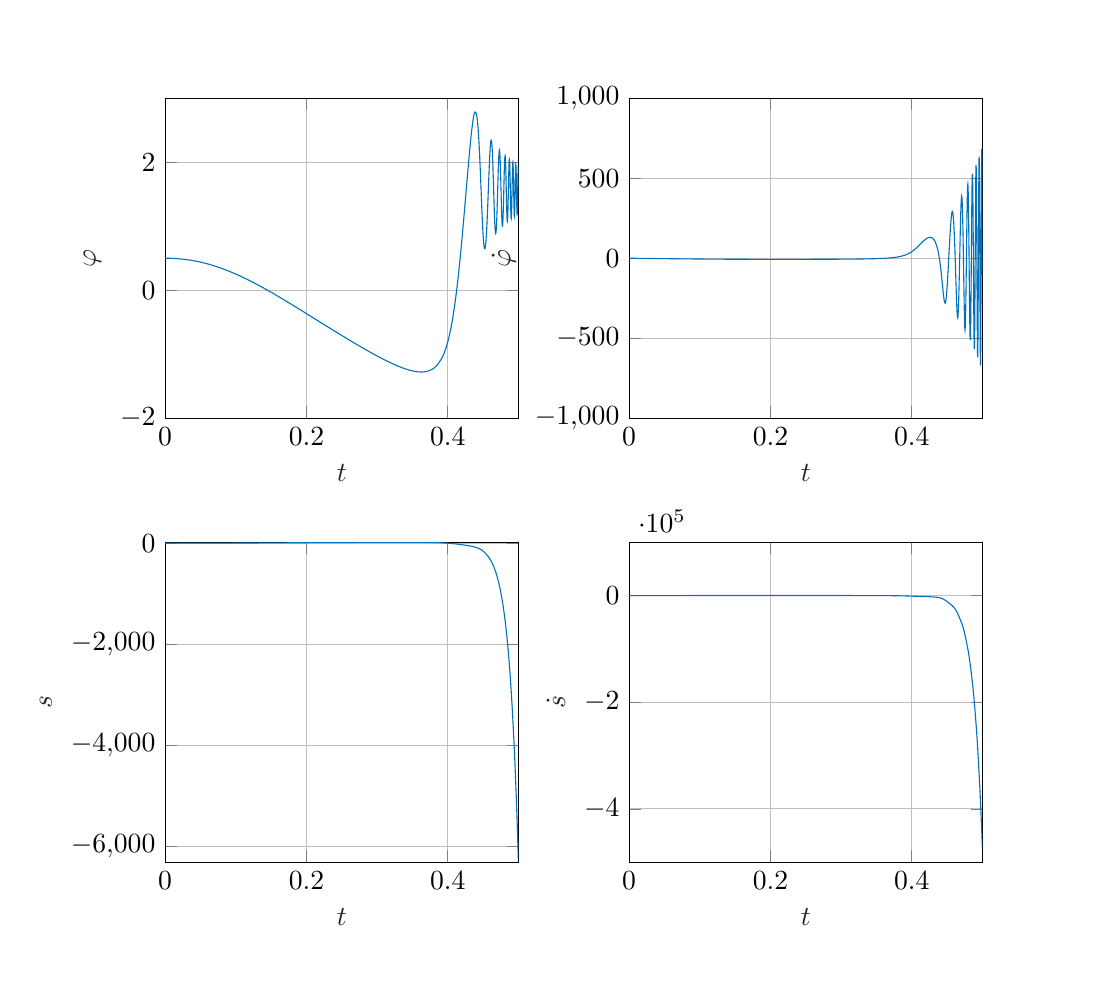
\begin{tikzpicture}

\begin{axis}[%
width=0.37\linewidth,
height=0.335\linewidth,
at={(0\linewidth,0.465\linewidth)},
scale only axis,
xmin=0,
xmax=0.5,
xlabel style={font=\color{white!15!black}},
xlabel={$t$},
ymin=-2,
ymax=3,
ylabel style={font=\color{white!15!black}},
ylabel={$\varphi$},
axis background/.style={fill=white},
xmajorgrids,
ymajorgrids
]
\addplot [color=mycolor1, forget plot]
  table[row sep=crcr]{%
0	0.5\\
8.48438300178876e-06	0.500000846580765\\
1.69687660035775e-05	0.500001689446444\\
2.54531490053663e-05	0.50000252859701\\
3.3937532007155e-05	0.500003364032437\\
7.63594470160989e-05	0.50000748548157\\
0.000118781362025043	0.500011514048311\\
0.000161203277033986	0.500015449729393\\
0.00020362519204293	0.500019292521549\\
0.000415734767087649	0.500037113034057\\
0.000627844342132368	0.500052610832792\\
0.000839953917177087	0.50006578550822\\
0.00105206349222181	0.500076636650251\\
0.0021126113674454	0.500096025024963\\
0.003173159242669	0.500057263251983\\
0.00423370711789259	0.499960299634229\\
0.00529425499311619	0.499805082569537\\
0.0105969943692342	0.498153585721244\\
0.0158997337453521	0.495038141020569\\
0.0212024731214701	0.490453059587372\\
0.0265052124975881	0.484394194982665\\
0.0364120174730008	0.469123364899346\\
0.0463188224484135	0.448702453103302\\
0.0562256274238261	0.423169996470867\\
0.0661324323992388	0.392624696469597\\
0.0786324323992388	0.347177746993189\\
0.0911324323992388	0.294423926462681\\
0.103632432399239	0.234929068715007\\
0.116132432399239	0.169410658430394\\
0.128632432399239	0.0986790744748462\\
0.141132432399239	0.023572631870427\\
0.153632432399239	-0.0550748719478153\\
0.166132432399239	-0.136482079027154\\
0.178632432399239	-0.219923970510903\\
0.191132432399239	-0.304757654813118\\
0.203632432399239	-0.390415876687432\\
0.216132432399239	-0.476400157138822\\
0.228632432399239	-0.562268740527925\\
0.241132432399239	-0.647607799030948\\
0.253632432399239	-0.731989916388328\\
0.266132432399239	-0.81495779477199\\
0.278632432399239	-0.895999910395063\\
0.291132432399239	-0.974446750987093\\
0.303632432399239	-1.04928560473401\\
0.316132432399239	-1.11910906637611\\
0.32357649043341	-1.15751745756789\\
0.331020548467582	-1.19280269855687\\
0.338464606501754	-1.22405926426946\\
0.345908664535925	-1.25005391471991\\
0.351576068558868	-1.26526721415433\\
0.357243472581811	-1.27541949595869\\
0.362910876604753	-1.27900241363958\\
0.368578280627696	-1.27382293592404\\
0.374245684650639	-1.25639621010666\\
0.379913088673581	-1.2226292856876\\
0.385580492696524	-1.16508929264558\\
0.391247896719467	-1.07125778966332\\
0.394597981403436	-0.991788426148544\\
0.397948066087406	-0.88829501922629\\
0.401298150771375	-0.754673636241166\\
0.404648235455345	-0.584490520703357\\
0.407324130448061	-0.418031943445409\\
0.410000025440778	-0.221325614474887\\
0.412675920433495	0.0072294714384501\\
0.415351815426212	0.267446597985779\\
0.418027710418929	0.557344974426085\\
0.420703605411646	0.873334366385971\\
0.423379500404363	1.20955410855697\\
0.426055395397079	1.55758487910159\\
0.428627017606333	1.89230268171942\\
0.431198639815586	2.2119917746023\\
0.43377026202484	2.49278705882107\\
0.436341884234094	2.70060203685728\\
0.437434593827094	2.75614011276924\\
0.438527303420093	2.78580776491703\\
0.439620013013093	2.78446646823768\\
0.440712722606093	2.74648333089041\\
0.441805432199093	2.66633402043821\\
0.442898141792093	2.53724715200933\\
0.443990851385093	2.35513595876513\\
0.445083560978093	2.12096364551726\\
0.445841080824213	1.93157271232622\\
0.446598600670332	1.72654868615444\\
0.447356120516452	1.51418565537168\\
0.448113640362572	1.3046892766852\\
0.448871160208691	1.10928024682466\\
0.449628680054811	0.938755411734919\\
0.45038619990093	0.802203218145666\\
0.45114371974705	0.70615863271522\\
0.451890878919254	0.654978257713285\\
0.452638038091459	0.649462707972198\\
0.453385197263663	0.690321084056097\\
0.454132356435867	0.776097976257471\\
0.45475282500609	0.879186760167892\\
0.455373293576312	1.0084121441809\\
0.455993762146534	1.15982269156496\\
0.456614230716756	1.32815612333122\\
0.457292365293331	1.52392082085339\\
0.457970499869905	1.72210105117802\\
0.45864863444648	1.91144069717184\\
0.459326769023055	2.0800999832101\\
0.459927169122086	2.20284341874497\\
0.460527569221118	2.29238839157616\\
0.46112796932015	2.34161784529828\\
0.461728369419182	2.34510548375616\\
0.462251727959639	2.30802307338477\\
0.462775086500096	2.23190649168629\\
0.463298445040554	2.11757617573678\\
0.463821803581011	1.9691023153199\\
0.464225837079452	1.83553095646686\\
0.464629870577892	1.69064865046527\\
0.465033904076333	1.54041420706481\\
0.465437937574773	1.39157537765999\\
0.465841971073214	1.25122680966905\\
0.466246004571654	1.12634048108649\\
0.466650038070095	1.02306348413423\\
0.467054071568535	0.946198429339811\\
0.467404639320517	0.903617787294012\\
0.467755207072498	0.885159475329713\\
0.46810577482448	0.891651081168369\\
0.468456342576461	0.92300718542691\\
0.468806910328443	0.978345528104904\\
0.469157478080424	1.05616443138873\\
0.469508045832406	1.15403575794701\\
0.469858613584387	1.26855958924811\\
0.470230976748853	1.4037226465294\\
0.470603339913318	1.54683204961233\\
0.470975703077784	1.6910712336296\\
0.47134806624225	1.82919012382744\\
0.471704689406547	1.94901013358139\\
0.472061312570845	2.05026435204408\\
0.472417935735142	2.12728780813019\\
0.47277455889944	2.17554825213122\\
0.473101382710734	2.1916517248151\\
0.473428206522029	2.17878620948541\\
0.473755030333323	2.13620155417638\\
0.474081854144617	2.06480716205073\\
0.474408677955912	1.96703994416329\\
0.474735501767206	1.84694002816438\\
0.4750623255785	1.71045107375882\\
0.475389149389795	1.56536309438798\\
0.475684885165112	1.43413967984246\\
0.475980620940429	1.31022114568688\\
0.476276356715746	1.20032741727891\\
0.476572092491063	1.11027549023747\\
0.476881457081637	1.04233039044343\\
0.47719082167221	1.00539015124596\\
0.477500186262784	1.00198538051035\\
0.477809550853358	1.03235710235677\\
0.478073982545808	1.08390558175474\\
0.478338414238259	1.15726415875268\\
0.47860284593071	1.24959414193568\\
0.47886727762316	1.35694474784599\\
0.479125483302954	1.47166618573541\\
0.479383688982748	1.59096834355408\\
0.479641894662541	1.70926281953763\\
0.479900100342335	1.82083779016995\\
0.480156369790976	1.91946955948683\\
0.480412639239616	2.00083184175779\\
0.480668908688257	2.06043068317632\\
0.480925178136898	2.09491245736174\\
0.481160338056472	2.1025304415713\\
0.481395497976047	2.08597192330909\\
0.481630657895621	2.04518130926967\\
0.481865817815196	1.98144111844277\\
0.48210097773477	1.89720393780222\\
0.482336137654345	1.79604453260753\\
0.482571297573919	1.68277229387828\\
0.482806457493494	1.56331663980747\\
0.483026786201826	1.45164487817787\\
0.483247114910157	1.34599605364966\\
0.483467443618489	1.25178240684856\\
0.483687772326821	1.17371678836712\\
0.483929023622707	1.11122699490457\\
0.484170274918594	1.07671218338098\\
0.48441152621448	1.07262346831847\\
0.484652777510367	1.09920851703197\\
0.484859378677873	1.14522303798346\\
0.48506597984538	1.21097920033848\\
0.485272581012886	1.29377675595654\\
0.485479182180392	1.38989081836333\\
0.485677156736859	1.49034235937657\\
0.485875131293326	1.59443808894362\\
0.486073105849793	1.69739583611155\\
0.48627108040626	1.79439171032205\\
0.486471854246824	1.88192303145583\\
0.486672628087388	1.95396407893934\\
0.486873401927951	2.00659590566126\\
0.487074175768515	2.0369681498661\\
0.487258884991867	2.04367204760678\\
0.487443594215219	2.02912527218943\\
0.48762830343857	1.99342397672826\\
0.487813012661922	1.93781157618627\\
0.487997721885274	1.86451037777469\\
0.488182431108626	1.77662328165982\\
0.488367140331978	1.67821376915721\\
0.488551849555329	1.57419696229365\\
0.488728022362953	1.47473172995353\\
0.488904195170576	1.37999353690336\\
0.489080367978199	1.2946939523027\\
0.489256540785823	1.22298352875739\\
0.489452180942729	1.16338319737797\\
0.489647821099636	1.12860895048662\\
0.489843461256543	1.12107957205129\\
0.490039101413449	1.14121936277531\\
0.490210992591485	1.1808168126147\\
0.49038288376952	1.23935589670067\\
0.490554774947555	1.31429928796526\\
0.490726666125591	1.40208764842475\\
0.490887187483913	1.49187656807328\\
0.491047708842235	1.58518667131196\\
0.491208230200557	1.67780866017196\\
0.491368751558879	1.76550352789341\\
0.491533261093837	1.84601272740612\\
0.491697770628795	1.91290254869502\\
0.491862280163752	1.9626180025473\\
0.49202678969871	1.99256698374678\\
0.492179300076172	2.00121069450343\\
0.492331810453634	1.99061860468183\\
0.492484320831096	1.96084723495946\\
0.492636831208559	1.91297763209764\\
0.492789341586021	1.84895491952014\\
0.492941851963483	1.77146522604948\\
0.493094362340945	1.6840185892643\\
0.493246872718407	1.59085716428491\\
0.493393680845894	1.50014674837979\\
0.493540488973381	1.41285492889386\\
0.493687297100868	1.33323224579182\\
0.493834105228355	1.26508328593934\\
0.493996986262518	1.20674812440627\\
0.494159867296681	1.17015549380413\\
0.494322748330845	1.15773324152166\\
0.494485629365008	1.17016775005391\\
0.494635123940643	1.20281593091699\\
0.494784618516278	1.25446533291959\\
0.494934113091912	1.32274184747459\\
0.495083607667547	1.40417646802452\\
0.495218561337975	1.48546563913183\\
0.495353515008403	1.57051593003372\\
0.495488468678831	1.65555316085269\\
0.495623422349259	1.73675785372895\\
0.495762134135602	1.81235458974247\\
0.495900845921946	1.87617301509273\\
0.49603955770829	1.92491814420484\\
0.496178269494633	1.95614063825002\\
0.496308391859062	1.96804041935881\\
0.49643851422349	1.9622186494885\\
0.496568636587918	1.9386072995304\\
0.496698758952347	1.89807886744127\\
0.496828881316775	1.84229590479555\\
0.496959003681204	1.77357331102994\\
0.497089126045632	1.69497502300529\\
0.497219248410061	1.61024167333121\\
0.497344985430044	1.52644226017218\\
0.497470722450027	1.44476567262266\\
0.497596459470011	1.36911654198952\\
0.497722196489994	1.30305642571109\\
0.497860545814171	1.24509003597738\\
0.497998895138348	1.20597026461978\\
0.498137244462524	1.18815143585216\\
0.498275593786701	1.19259783761752\\
0.498410113417048	1.21797450776269\\
0.498544633047396	1.26305507748755\\
0.498679152677743	1.32562460372679\\
0.498813672308091	1.40222135436467\\
0.498930137774753	1.47652800686836\\
0.499046603241416	1.5549525252264\\
0.499163068708078	1.63405965761012\\
0.499279534174741	1.7103449593887\\
0.499399813169087	1.78255034945961\\
0.499520092163433	1.84448574929509\\
0.49964037115778	1.89300361797252\\
0.499760650152126	1.92571403565132\\
0.499820487614095	1.93554758035625\\
0.499880325076063	1.94087915039368\\
0.499940162538032	1.94161534855566\\
0.5	1.93772053231314\\
};
\end{axis}

\begin{axis}[%
width=0.37\linewidth,
height=0.335\linewidth,
at={(0.486\linewidth,0.465\linewidth)},
scale only axis,
xmin=0,
xmax=0.5,
xlabel style={font=\color{white!15!black}},
xlabel={$t$},
ymin=-1000,
ymax=1000,
ylabel style={font=\color{white!15!black}},
ylabel={$\dot\varphi$},
axis background/.style={fill=white},
xmajorgrids,
ymajorgrids
]
\addplot [color=mycolor1, forget plot]
  table[row sep=crcr]{%
0	0.1\\
8.48438300178876e-06	0.0995621279977272\\
1.69687660035775e-05	0.0991242529186282\\
2.54531490053663e-05	0.0986863747624824\\
3.3937532007155e-05	0.09824849352907\\
7.63594470160989e-05	0.0960590411953524\\
0.000118781362025043	0.0938695118973062\\
0.000161203277033986	0.0916799056080676\\
0.00020362519204293	0.089490222301117\\
0.000415734767087649	0.0785406495967114\\
0.000627844342132368	0.0675891476699279\\
0.000839953917177087	0.0566357135944657\\
0.00105206349222181	0.0456803446606259\\
0.0021126113674454	-0.00912560232320385\\
0.003173159242669	-0.0639802021286915\\
0.00423370711789259	-0.118883546876985\\
0.00529425499311619	-0.173835589567215\\
0.0105969943692342	-0.449314636809541\\
0.0158997337453521	-0.725922155331838\\
0.0212024731214701	-1.00348726889089\\
0.0265052124975881	-1.28174368838713\\
0.0364120174730008	-1.80216084660075\\
0.0463188224484135	-2.32032489282086\\
0.0562256274238261	-2.83182966639347\\
0.0661324323992388	-3.33142523049619\\
0.0786324323992388	-3.93566243357224\\
0.0911324323992388	-4.49885748388692\\
0.103632432399239	-5.00987691556609\\
0.116132432399239	-5.46024898257466\\
0.128632432399239	-5.84442856044327\\
0.141132432399239	-6.16125596589939\\
0.153632432399239	-6.41269244062608\\
0.166132432399239	-6.6031772743647\\
0.178632432399239	-6.73898160500653\\
0.191132432399239	-6.82663549827641\\
0.203632432399239	-6.87200592574315\\
0.216132432399239	-6.87986753102019\\
0.228632432399239	-6.85357114056295\\
0.241132432399239	-6.79434220827268\\
0.253632432399239	-6.70068164762185\\
0.266132432399239	-6.56806847162529\\
0.278632432399239	-6.38782222453769\\
0.291132432399239	-6.14523309350606\\
0.303632432399239	-5.81137016498154\\
0.316132432399239	-5.33983657133668\\
0.32357649043341	-4.96485428714562\\
0.331020548467582	-4.49086871639498\\
0.338464606501754	-3.87924017340137\\
0.345908664535925	-3.07234091823543\\
0.351576068558868	-2.27408131207649\\
0.357243472581811	-1.25890189883115\\
0.362910876604753	0.0655021862100593\\
0.368578280627696	1.84614631154036\\
0.374245684650639	4.30972838311322\\
0.379913088673581	7.80633437831683\\
0.385580492696524	12.9580195398939\\
0.391247896719467	20.7187389629331\\
0.394597981403436	27.0391901201466\\
0.397948066087406	35.0537970607726\\
0.401298150771375	44.9959424112651\\
0.404648235455345	56.9212546124119\\
0.407324130448061	67.7537418865729\\
0.410000025440778	79.3978045906332\\
0.412675920433495	91.3528725522459\\
0.415351815426212	102.970773688769\\
0.418027710418929	113.494306151037\\
0.420703605411646	122.271936982202\\
0.423379500404363	128.476895430324\\
0.426055395397079	130.980543310054\\
0.428627017606333	128.4387953553\\
0.431198639815586	118.505645976849\\
0.43377026202484	97.6002696446668\\
0.436341884234094	61.2093443942558\\
0.437434593827094	39.7178071082249\\
0.438527303420093	13.7999724222724\\
0.439620013013093	-17.0869810307142\\
0.440712722606093	-53.3584406715164\\
0.441805432199093	-95.0080414806239\\
0.442898141792093	-141.722373581869\\
0.443990851385093	-190.903469074252\\
0.445083560978093	-236.677076620709\\
0.445841080824213	-261.937324481336\\
0.446598600670332	-277.707890476863\\
0.447356120516452	-280.847400114921\\
0.448113640362572	-269.541816007579\\
0.448871160208691	-243.57575077937\\
0.449628680054811	-204.519307858291\\
0.45038619990093	-154.877982580441\\
0.45114371974705	-98.0183285359048\\
0.451890878919254	-38.0448933234886\\
0.452638038091459	23.7287648316001\\
0.453385197263663	85.0171094530737\\
0.454132356435867	143.490022088251\\
0.45475282500609	188.159571970535\\
0.455373293576312	227.384678076135\\
0.455993762146534	259.187771008138\\
0.456614230716756	281.582466512661\\
0.457292365293331	293.138330819947\\
0.457970499869905	288.766948239742\\
0.45864863444648	266.88236774234\\
0.459326769023055	227.427718465139\\
0.459927169122086	178.61646680528\\
0.460527569221118	117.454521713314\\
0.46112796932015	45.5017571436056\\
0.461728369419182	-34.5925067804413\\
0.462251727959639	-108.363402344339\\
0.462775086500096	-182.543507420328\\
0.463298445040554	-252.483723744417\\
0.463821803581011	-312.169291061884\\
0.464225837079452	-346.863301783167\\
0.464629870577892	-367.999964407335\\
0.465033904076333	-373.017805352481\\
0.465437937574773	-360.600141060874\\
0.465841971073214	-330.740938584433\\
0.466246004571654	-284.741755609551\\
0.466650038070095	-224.891884824796\\
0.467054071568535	-154.428615953957\\
0.467404639320517	-87.4659191198162\\
0.467755207072498	-17.2445571047653\\
0.46810577482448	54.0365829483908\\
0.468456342576461	124.174651885711\\
0.468806910328443	190.97182159063\\
0.469157478080424	251.97404770103\\
0.469508045832406	304.642357454436\\
0.469858613584387	346.506007779229\\
0.470230976748853	376.576935508035\\
0.470603339913318	389.168600950777\\
0.470975703077784	382.453917587499\\
0.47134806624225	355.925845731921\\
0.471704689406547	312.489520994698\\
0.472061312570845	252.469590557808\\
0.472417935735142	177.833757136563\\
0.47277455889944	91.5570598566807\\
0.473101382710734	5.29710750654834\\
0.473428206522029	-84.7750161485551\\
0.473755030333323	-174.835046240442\\
0.474081854144617	-260.327535583384\\
0.474408677955912	-336.174705467665\\
0.474735501767206	-396.235363380046\\
0.4750623255785	-434.847414932368\\
0.475389149389795	-447.731246057825\\
0.475684885165112	-435.066259061388\\
0.475980620940429	-399.085952175786\\
0.476276356715746	-341.322289510053\\
0.476572092491063	-265.161562442579\\
0.476881457081637	-170.674719761751\\
0.47719082167221	-66.003252029525\\
0.477500186262784	43.2674928931207\\
0.477809550853358	151.17410007336\\
0.478073982545808	237.873938149161\\
0.478338414238259	315.479460436982\\
0.47860284593071	380.133073899807\\
0.47886727762316	428.337335038456\\
0.479125483302954	456.639765169519\\
0.479383688982748	463.935982112492\\
0.479641894662541	448.881769023902\\
0.479900100342335	411.611477453307\\
0.480156369790976	353.970978126085\\
0.480412639239616	277.716466682439\\
0.480668908688257	185.819737311454\\
0.480925178136898	82.2979371010603\\
0.481160338056472	-18.9833587477494\\
0.481395497976047	-122.313121055194\\
0.481630657895621	-223.172200836591\\
0.481865817815196	-316.605588876002\\
0.48210097773477	-397.429837405636\\
0.482336137654345	-459.929281668392\\
0.482571297573919	-499.129033789375\\
0.482806457493494	-511.527995224942\\
0.483026786201826	-497.157397410165\\
0.483247114910157	-457.620526230259\\
0.483467443618489	-394.546469016459\\
0.483687772326821	-311.332563749125\\
0.483929023622707	-202.470487318515\\
0.484170274918594	-81.0103423667197\\
0.48441152621448	46.2123130748686\\
0.484652777510367	171.827572651962\\
0.484859378677873	272.584803477229\\
0.48506597984538	362.186047589727\\
0.485272581012886	436.05635848276\\
0.485479182180392	490.193393460973\\
0.485677156736859	520.474108074078\\
0.485875131293326	527.181931800239\\
0.486073105849793	509.132664416561\\
0.48627108040626	466.709187078755\\
0.486471854246824	400.498602066408\\
0.486672628087388	313.440252640539\\
0.486873401927951	209.168305471114\\
0.487074175768515	92.4397254544091\\
0.487258884991867	-21.3239832849483\\
0.487443594215219	-136.587541178051\\
0.48762830343857	-248.310933047562\\
0.487813012661922	-351.182603601305\\
0.487997721885274	-439.823662022568\\
0.488182431108626	-508.546685435051\\
0.488367140331978	-552.49258099747\\
0.488551849555329	-568.294143370511\\
0.488728022362953	-555.501793615764\\
0.488904195170576	-515.402907224469\\
0.489080367978199	-449.578233246472\\
0.489256540785823	-361.421155056529\\
0.489452180942729	-242.962619363546\\
0.489647821099636	-109.41445340162\\
0.489843461256543	31.6077041813379\\
0.490039101413449	171.831737342889\\
0.490210992591485	287.849081223145\\
0.49038288376952	391.33185585701\\
0.490554774947555	476.842888081702\\
0.490726666125591	539.695506154918\\
0.490887187483913	574.533090355853\\
0.491047708842235	583.754393955217\\
0.491208230200557	566.142992478762\\
0.491368751558879	522.116673925726\\
0.491533261093837	451.440128135775\\
0.491697770628795	357.677362329905\\
0.491862280163752	244.849775552293\\
0.49202678969871	118.184218350209\\
0.492179300076172	-6.45956394290344\\
0.492331810453634	-132.927163080166\\
0.492484320831096	-255.723765998\\
0.492636831208559	-369.169888154892\\
0.492789341586021	-467.607284620921\\
0.492941851963483	-545.171947942462\\
0.493094362340945	-596.851044925534\\
0.493246872718407	-619.116807364869\\
0.493393680845894	-610.920759391325\\
0.493540488973381	-573.303808009052\\
0.493687297100868	-507.651714218302\\
0.493834105228355	-417.247954381945\\
0.493996986262518	-293.596969867353\\
0.494159867296681	-152.15911725037\\
0.494322748330845	-0.915395167637769\\
0.494485629365008	151.376229945201\\
0.494635123940643	284.56192182649\\
0.494784618516278	404.483902626614\\
0.494934113091912	504.572812299172\\
0.495083607667547	579.175620037845\\
0.495218561337975	620.769881566839\\
0.495353515008403	635.084370429568\\
0.495488468678831	620.729527179212\\
0.495623422349259	578.005324904973\\
0.495762134135602	506.333089406236\\
0.495900845921946	409.369241116121\\
0.49603955770829	291.290761896172\\
0.496178269494633	157.565139185944\\
0.496308391859062	23.4226155393676\\
0.49643851422349	-113.592877285811\\
0.496568636587918	-247.565084266143\\
0.496698758952347	-372.426438366947\\
0.496828881316775	-482.172955168111\\
0.496959003681204	-570.6385348894\\
0.497089126045632	-632.494669131911\\
0.497219248410061	-663.873803742744\\
0.497344985430044	-663.037669865384\\
0.497470722450027	-630.827965437774\\
0.497596459470011	-568.297926387396\\
0.497722196489994	-478.492267141347\\
0.497860545814171	-353.558075563662\\
0.497998895138348	-207.958828345763\\
0.498137244462524	-49.7165408154131\\
0.498275593786701	112.237174781146\\
0.498410113417048	264.689402625373\\
0.498544633047396	403.789473086329\\
0.498679152677743	521.445347571021\\
0.498813672308091	610.652546822313\\
0.498930137774753	660.423519392505\\
0.499046603241416	681.499655208139\\
0.499163068708078	672.231406566336\\
0.499279534174741	632.710640990138\\
0.499399813169087	561.815098534162\\
0.499520092163433	463.17964666203\\
0.49964037115778	341.076874044305\\
0.499760650152126	201.194378408766\\
0.499820487614095	127.025375538658\\
0.499880325076063	50.8847925518914\\
0.499940162538032	-26.3411641757147\\
0.5	-103.743798848226\\
};
\end{axis}

\begin{axis}[%
width=0.37\linewidth,
height=0.335\linewidth,
at={(0\linewidth,0\linewidth)},
scale only axis,
xmin=0,
xmax=0.5,
xlabel style={font=\color{white!15!black}},
xlabel={$t$},
ymin=-6311.0875775132,
ymax=18.5759168621428,
ylabel style={font=\color{white!15!black}},
ylabel={$s$},
axis background/.style={fill=white},
xmajorgrids,
ymajorgrids
]
\addplot [color=mycolor1, forget plot]
  table[row sep=crcr]{%
0	0.1\\
8.48438300178876e-06	0.10000086975016\\
1.69687660035775e-05	0.10000178212425\\
2.54531490053663e-05	0.100002737122589\\
3.3937532007155e-05	0.100003734745493\\
7.63594470160989e-05	0.100009362239606\\
0.000118781362025043	0.100016055395443\\
0.000161203277033986	0.100023814252613\\
0.00020362519204293	0.10003263885068\\
0.000415734767087649	0.100092749336118\\
0.000627844342132368	0.10017950925446\\
0.000839953917177087	0.100292923503079\\
0.00105206349222181	0.100432996951218\\
0.0021126113674454	0.101533419966972\\
0.003173159242669	0.103301036892204\\
0.00423370711789259	0.105736422378455\\
0.00529425499311619	0.108840128244388\\
0.0105969943692342	0.134399070571342\\
0.0158997337453521	0.176734704088627\\
0.0212024731214701	0.235882770316045\\
0.0265052124975881	0.311848167318078\\
0.0364120174730008	0.498667028591176\\
0.0463188224484135	0.743574076120169\\
0.0562256274238261	1.04555014464422\\
0.0661324323992388	1.40283671814609\\
0.0786324323992388	1.92874701904241\\
0.0911324323992388	2.53278081789284\\
0.103632432399239	3.20764081086703\\
0.116132432399239	3.94477027595542\\
0.128632432399239	4.7350004503038\\
0.141132432399239	5.56935290148405\\
0.153632432399239	6.43917494417705\\
0.166132432399239	7.33656469931123\\
0.178632432399239	8.25433459245914\\
0.191132432399239	9.18610647535863\\
0.203632432399239	10.1261324147659\\
0.216132432399239	11.0691667466296\\
0.228632432399239	12.0102498289532\\
0.241132432399239	12.9443496709169\\
0.253632432399239	13.8655110626749\\
0.266132432399239	14.7664751617777\\
0.278632432399239	15.6376157199209\\
0.291132432399239	16.4662151806476\\
0.303632432399239	17.2286156286717\\
0.316132432399239	17.8867799671669\\
0.32357649043341	18.2057011738716\\
0.331020548467582	18.4460236743825\\
0.338464606501754	18.5759168621428\\
0.345908664535925	18.549095436279\\
0.351576068558868	18.3837485741367\\
0.357243472581811	18.0487480822239\\
0.362910876604753	17.4869439191627\\
0.368578280627696	16.6211992970562\\
0.374245684650639	15.349074006837\\
0.379913088673581	13.5401951093523\\
0.385580492696524	11.0318669696112\\
0.391247896719467	7.62316769652163\\
0.394597981403436	5.09421444776037\\
0.397948066087406	2.12934257019862\\
0.401298150771375	-1.30933642117656\\
0.404648235455345	-5.24908041138895\\
0.407324130448061	-8.76634070033528\\
0.410000025440778	-12.6140785223684\\
0.412675920433495	-16.7889739857023\\
0.415351815426212	-21.2828205072734\\
0.418027710418929	-26.087409006735\\
0.420703605411646	-31.1998720330259\\
0.423379500404363	-36.631167419506\\
0.426055395397079	-42.4120089874738\\
0.428627017606333	-48.3535976417553\\
0.431198639815586	-54.7623459579019\\
0.43377026202484	-61.8071890932256\\
0.436341884234094	-69.7618438959873\\
0.437434593827094	-73.5099340408867\\
0.438527303420093	-77.536913137831\\
0.439620013013093	-81.8941086099012\\
0.440712722606093	-86.643024101293\\
0.441805432199093	-91.8564107659878\\
0.442898141792093	-97.6173413861831\\
0.443990851385093	-104.020308024193\\
0.445083560978093	-111.172967822271\\
0.445841080824213	-116.63174796411\\
0.446598600670332	-122.542485726507\\
0.447356120516452	-128.939796607688\\
0.448113640362572	-135.853272359717\\
0.448871160208691	-143.307309817346\\
0.449628680054811	-151.321344289076\\
0.45038619990093	-159.909590269776\\
0.45114371974705	-169.080706043399\\
0.451890878919254	-178.702601128028\\
0.452638038091459	-188.901073897537\\
0.453385197263663	-199.679570983506\\
0.454132356435867	-211.042131516306\\
0.45475282500609	-220.925822147909\\
0.455373293576312	-231.220396232938\\
0.455993762146534	-241.932398071583\\
0.456614230716756	-253.071513641022\\
0.457292365293331	-265.750396749345\\
0.457970499869905	-278.977806120112\\
0.45864863444648	-292.783771327405\\
0.459326769023055	-307.208158535483\\
0.459927169122086	-320.534342284054\\
0.460527569221118	-334.422372508896\\
0.46112796932015	-348.91700582564\\
0.461728369419182	-364.069194492513\\
0.462251727959639	-377.857069740355\\
0.462775086500096	-392.226102304254\\
0.463298445040554	-407.216982230567\\
0.463821803581011	-422.871240960813\\
0.464225837079452	-435.436059689976\\
0.464629870577892	-448.438634229101\\
0.465033904076333	-461.895622367429\\
0.465437937574773	-475.821562252332\\
0.465841971073214	-490.229029605028\\
0.466246004571654	-505.128998430792\\
0.466650038070095	-520.530497668406\\
0.467054071568535	-536.440533718962\\
0.467404639320517	-550.661658351405\\
0.467755207072498	-565.273325456264\\
0.46810577482448	-580.278601665386\\
0.468456342576461	-595.680576059022\\
0.468806910328443	-611.482552625876\\
0.469157478080424	-627.688082545161\\
0.469508045832406	-644.301511613313\\
0.469858613584387	-661.328344418901\\
0.470230976748853	-679.874204421318\\
0.470603339913318	-698.90386346134\\
0.470975703077784	-718.429434407202\\
0.47134806624225	-738.46610085979\\
0.471704689406547	-758.151544736657\\
0.472061312570845	-778.339992654578\\
0.472417935735142	-799.051551867353\\
0.47277455889944	-820.308773110279\\
0.473101382710734	-840.289775784165\\
0.473428206522029	-860.769366008655\\
0.473755030333323	-881.768188617556\\
0.474081854144617	-903.307432630678\\
0.474408677955912	-925.40833156694\\
0.474735501767206	-948.09204710386\\
0.4750623255785	-971.378726681055\\
0.475389149389795	-995.28672846135\\
0.475684885165112	-1017.46984534052\\
0.475980620940429	-1040.18629157342\\
0.476276356715746	-1063.44561157116\\
0.476572092491063	-1087.25558415787\\
0.476881457081637	-1112.75926292582\\
0.47719082167221	-1138.87949621221\\
0.477500186262784	-1165.6223639747\\
0.477809550853358	-1192.99363121848\\
0.478073982545808	-1216.89203665873\\
0.478338414238259	-1241.25803296822\\
0.47860284593071	-1266.0963621988\\
0.47886727762316	-1291.41279008721\\
0.479125483302954	-1316.60107632403\\
0.479383688982748	-1342.25909789161\\
0.479641894662541	-1368.39557467099\\
0.479900100342335	-1395.02091489214\\
0.480156369790976	-1421.94169854258\\
0.480412639239616	-1449.36848218943\\
0.480668908688257	-1477.31533246782\\
0.480925178136898	-1505.79763262218\\
0.481160338056472	-1532.41886169669\\
0.481395497976047	-1559.51779896062\\
0.481630657895621	-1587.10786740429\\
0.481865817815196	-1615.20259133717\\
0.48210097773477	-1643.81535317557\\
0.482336137654345	-1672.95937057036\\
0.482571297573919	-1702.64718325648\\
0.482806457493494	-1732.89024641467\\
0.483026786201826	-1761.73899983842\\
0.483247114910157	-1791.09218150574\\
0.483467443618489	-1820.95672385906\\
0.483687772326821	-1851.33850269512\\
0.483929023622707	-1885.20467197324\\
0.484170274918594	-1919.70330394314\\
0.48441152621448	-1954.84005872431\\
0.484652777510367	-1990.62034042166\\
0.484859378677873	-2021.77733301532\\
0.48506597984538	-2053.41412837973\\
0.485272581012886	-2085.53496755608\\
0.485479182180392	-2118.14485015082\\
0.485677156736859	-2149.85731416321\\
0.485875131293326	-2182.02988239344\\
0.486073105849793	-2214.66918522598\\
0.48627108040626	-2247.7829387002\\
0.486471854246824	-2281.85835235786\\
0.486672628087388	-2316.44040517282\\
0.486873401927951	-2351.53976022499\\
0.487074175768515	-2387.16794458303\\
0.487258884991867	-2420.42287331397\\
0.487443594215219	-2454.14538434083\\
0.48762830343857	-2488.34539241924\\
0.487813012661922	-2523.03282128606\\
0.487997721885274	-2558.21745616818\\
0.488182431108626	-2593.90894117991\\
0.488367140331978	-2630.11644457528\\
0.488551849555329	-2666.84840054161\\
0.488728022362953	-2702.37853000493\\
0.488904195170576	-2738.3990341518\\
0.489080367978199	-2774.91549181274\\
0.489256540785823	-2811.93274181319\\
0.489452180942729	-2853.63253676963\\
0.489647821099636	-2895.9606818881\\
0.489843461256543	-2938.92222632947\\
0.490039101413449	-2982.52198880297\\
0.490210992591485	-3021.35971068366\\
0.49038288376952	-3060.69743001746\\
0.490554774947555	-3100.53904050252\\
0.490726666125591	-3140.88903654677\\
0.490887187483913	-3179.03363894837\\
0.491047708842235	-3217.63067950716\\
0.491208230200557	-3256.68541938266\\
0.491368751558879	-3296.20388520678\\
0.491533261093837	-3337.19234227539\\
0.491697770628795	-3378.68261698157\\
0.491862280163752	-3420.68309191187\\
0.49202678969871	-3463.20277365541\\
0.492179300076172	-3503.09312092874\\
0.492331810453634	-3543.44553043932\\
0.492484320831096	-3584.26785672622\\
0.492636831208559	-3625.5679492043\\
0.492789341586021	-3667.35354903787\\
0.492941851963483	-3709.63228978909\\
0.493094362340945	-3752.41145691812\\
0.493246872718407	-3795.69780427407\\
0.493393680845894	-3837.85062808411\\
0.493540488973381	-3880.48442874513\\
0.493687297100868	-3923.6039306521\\
0.493834105228355	-3967.21329631477\\
0.493996986262518	-4016.17491072616\\
0.494159867296681	-4065.74890437087\\
0.494322748330845	-4115.93970421131\\
0.494485629365008	-4166.75151897869\\
0.494635123940643	-4213.93751516223\\
0.494784618516278	-4261.65363185062\\
0.494934113091912	-4309.90357750856\\
0.495083607667547	-4358.69156344099\\
0.495218561337975	-4403.20009877496\\
0.495353515008403	-4448.15478243658\\
0.495488468678831	-4493.55992169114\\
0.495623422349259	-4539.42039704226\\
0.495762134135602	-4587.03815894754\\
0.495900845921946	-4635.14889772662\\
0.49603955770829	-4683.75935220131\\
0.496178269494633	-4732.87673929133\\
0.496308391859062	-4779.42017913726\\
0.49643851422349	-4826.42275286373\\
0.496568636587918	-4873.89096598783\\
0.496698758952347	-4921.83132639776\\
0.496828881316775	-4970.25026475997\\
0.496959003681204	-5019.15413348056\\
0.497089126045632	-5068.54902349816\\
0.497219248410061	-5118.44062396826\\
0.497344985430044	-5167.12765924343\\
0.497470722450027	-5216.2879579399\\
0.497596459470011	-5265.92564249281\\
0.497722196489994	-5316.04438803228\\
0.497860545814171	-5371.75024023023\\
0.497998895138348	-5428.0467005701\\
0.498137244462524	-5484.93763552424\\
0.498275593786701	-5542.42670262255\\
0.498410113417048	-5598.90137975344\\
0.498544633047396	-5655.94841220472\\
0.498679152677743	-5713.57147811566\\
0.498813672308091	-5771.7746968836\\
0.498930137774753	-5822.63845348533\\
0.499046603241416	-5873.94377399681\\
0.499163068708078	-5925.69428383819\\
0.499279534174741	-5977.8940574519\\
0.499399813169087	-6032.27936235559\\
0.499520092163433	-6087.15384221186\\
0.49964037115778	-6142.52314098854\\
0.499760650152126	-6198.3932941309\\
0.499820487614095	-6226.37659611306\\
0.499880325076063	-6254.48620709223\\
0.499940162538032	-6282.72293105246\\
0.5	-6311.0875775132\\
};
\end{axis}

\begin{axis}[%
width=0.37\linewidth,
height=0.335\linewidth,
at={(0.486\linewidth,0\linewidth)},
scale only axis,
xmin=0,
xmax=0.5,
xlabel style={font=\color{white!15!black}},
xlabel={$t$},
ymin=-500000,
ymax=100000,
ylabel style={font=\color{white!15!black}},
ylabel={$\dot s$},
axis background/.style={fill=white},
xmajorgrids,
ymajorgrids
]
\addplot [color=mycolor1, forget plot]
  table[row sep=crcr]{%
0	0.1\\
8.48438300178876e-06	0.105023791580583\\
1.69687660035775e-05	0.110047620591048\\
2.54531490053663e-05	0.115071487023523\\
3.3937532007155e-05	0.12009539087013\\
7.63594470160989e-05	0.145215471038926\\
0.000118781362025043	0.170336485375413\\
0.000161203277033986	0.195458432887303\\
0.00020362519204293	0.220581312578158\\
0.000415734767087649	0.346209658550615\\
0.000627844342132368	0.471861157145267\\
0.000839953917177087	0.597535679135255\\
0.00105206349222181	0.723233092693567\\
0.0021126113674454	1.35205873637781\\
0.003173159242669	1.98143539745121\\
0.00423370711789259	2.61134365870619\\
0.00529425499311619	3.24176245828183\\
0.0105969943692342	6.40066331006839\\
0.0158997337453521	9.56821340170292\\
0.0212024731214701	12.7399184821314\\
0.0265052124975881	15.9102641539655\\
0.0364120174730008	21.8069530026881\\
0.0463188224484135	27.6241534808873\\
0.0562256274238261	33.3025850894427\\
0.0661324323992388	38.7784777483155\\
0.0786324323992388	45.2975400611124\\
0.0911324323992388	51.2663206994979\\
0.103632432399239	56.5893609421171\\
0.116132432399239	61.2077684744666\\
0.128632432399239	65.0983520469285\\
0.141132432399239	68.2794142198318\\
0.153632432399239	70.7933758991519\\
0.166132432399239	72.6981882580906\\
0.178632432399239	74.0608637449828\\
0.191132432399239	74.9427092386617\\
0.203632432399239	75.3907348083633\\
0.216132432399239	75.433243256479\\
0.228632432399239	75.0739238533156\\
0.241132432399239	74.2890298149074\\
0.253632432399239	72.9981675725179\\
0.266132432399239	71.0495944379649\\
0.278632432399239	68.1609985073098\\
0.291132432399239	63.9519361791519\\
0.303632432399239	57.5110539641174\\
0.316132432399239	47.1817964856138\\
0.32357649043341	38.0897344416705\\
0.331020548467582	25.632944142938\\
0.338464606501754	8.18592503301324\\
0.345908664535925	-16.6872476422907\\
0.351576068558868	-42.7121897741866\\
0.357243472581811	-77.2682423703267\\
0.362910876604753	-123.378838253885\\
0.368578280627696	-184.991893404289\\
0.374245684650639	-266.865001588411\\
0.379913088673581	-375.341047586319\\
0.385580492696524	-516.354726866488\\
0.391247896719467	-694.39470903348\\
0.394597981403436	-817.970407343207\\
0.397948066087406	-953.963854810353\\
0.401298150771375	-1100.02555648322\\
0.404648235455345	-1252.71603472894\\
0.407324130448061	-1376.58309119009\\
0.410000025440778	-1499.56805574364\\
0.412675920433495	-1620.03583365678\\
0.415351815426212	-1737.49899111766\\
0.418027710418929	-1852.99362125866\\
0.420703605411646	-1969.32834226328\\
0.423379500404363	-2092.28749495303\\
0.426055395397079	-2231.32507530386\\
0.428627017606333	-2393.60426760313\\
0.431198639815586	-2603.64987890053\\
0.43377026202484	-2894.49992900063\\
0.436341884234094	-3315.80392250285\\
0.437434593827094	-3550.38379258259\\
0.438527303420093	-3827.96864617145\\
0.439620013013093	-4156.80571737207\\
0.440712722606093	-4546.33216628462\\
0.441805432199093	-5006.74425321627\\
0.442898141792093	-5550.07779778667\\
0.443990851385093	-6186.95282668049\\
0.445083560978093	-6924.6974774058\\
0.445841080824213	-7496.91911939251\\
0.446598600670332	-8116.58105145934\\
0.447356120516452	-8779.25774472311\\
0.448113640362572	-9478.51888639831\\
0.448871160208691	-10206.6777300354\\
0.449628680054811	-10956.0304987093\\
0.45038619990093	-11719.9274355768\\
0.45114371974705	-12493.465036571\\
0.451890878919254	-13262.9669069041\\
0.452638038091459	-14037.2347101479\\
0.453385197263663	-14815.91582384\\
0.454132356435867	-15600.5402748587\\
0.45475282500609	-16258.863525746\\
0.455373293576312	-16925.9938697117\\
0.455993762146534	-17605.7754069749\\
0.456614230716756	-18303.4033602632\\
0.457292365293331	-19093.9109563299\\
0.457970499869905	-19923.7368615261\\
0.45864863444648	-20804.7050574712\\
0.459326769023055	-21749.8806091513\\
0.459927169122086	-22651.1718020407\\
0.460527569221118	-23623.0451959246\\
0.46112796932015	-24674.9288331047\\
0.461728369419182	-25815.2844472485\\
0.462251727959639	-26887.164956467\\
0.462775086500096	-28036.0693480035\\
0.463298445040554	-29264.3792072556\\
0.463821803581011	-30571.7802576764\\
0.464225837079452	-31633.4173100566\\
0.464629870577892	-32737.7234124251\\
0.465033904076333	-33880.8982322836\\
0.465437937574773	-35058.3106389059\\
0.465841971073214	-36264.885958773\\
0.466246004571654	-37495.5320146182\\
0.466650038070095	-38745.7092895242\\
0.467054071568535	-40011.8662240413\\
0.467404639320517	-41121.4481428041\\
0.467755207072498	-42240.0375050588\\
0.46810577482448	-43367.1605043422\\
0.468456342576461	-44503.1201621605\\
0.468806910328443	-45648.9122926608\\
0.469157478080424	-46806.0773050977\\
0.469508045832406	-47977.0024177851\\
0.469858613584387	-49164.9877599294\\
0.470230976748853	-50450.1008596766\\
0.470603339913318	-51764.9755896229\\
0.470975703077784	-53116.3130666876\\
0.47134806624225	-54511.4152698987\\
0.471704689406547	-55895.5360964479\\
0.472061312570845	-57333.3811584136\\
0.472417935735142	-58831.2803390492\\
0.47277455889944	-60394.7869807179\\
0.473101382710734	-61889.2714180059\\
0.473428206522029	-63445.9911976636\\
0.473755030333323	-65067.1447617609\\
0.474081854144617	-66753.5626670935\\
0.474408677955912	-68504.7817959433\\
0.474735501767206	-70318.9722742576\\
0.4750623255785	-72192.6109973791\\
0.475389149389795	-74120.4713766568\\
0.475684885165112	-75906.377384169\\
0.475980620940429	-77726.357019977\\
0.476276356715746	-79575.4247051361\\
0.476572092491063	-81449.2274395986\\
0.476881457081637	-83432.1268360029\\
0.47719082167221	-85435.2548546959\\
0.477500186262784	-87456.9189137228\\
0.477809550853358	-89497.3463620202\\
0.478073982545808	-91257.63376333\\
0.478338414238259	-93034.6998837188\\
0.47860284593071	-94831.3110621454\\
0.47886727762316	-96651.2554299391\\
0.479125483302954	-98455.263086805\\
0.479383688982748	-100290.834808758\\
0.479641894662541	-102163.373264924\\
0.479900100342335	-104078.513922486\\
0.480156369790976	-106026.940965258\\
0.480412639239616	-108028.222955482\\
0.480668908688257	-110087.238748172\\
0.480925178136898	-112207.998828392\\
0.481160338056472	-114211.082562555\\
0.481395497976047	-116270.756990786\\
0.481630657895621	-118388.084456753\\
0.481865817815196	-120562.99883798\\
0.48210097773477	-122794.429770453\\
0.482336137654345	-125080.341580882\\
0.482571297573919	-127417.598885242\\
0.482806457493494	-129802.033035477\\
0.483026786201826	-132074.614688552\\
0.483247114910157	-134380.172102488\\
0.483467443618489	-136714.633086918\\
0.483687772326821	-139074.439036843\\
0.483929023622707	-141684.066681336\\
0.484170274918594	-144317.694869397\\
0.48441152621448	-146973.667731213\\
0.484652777510367	-149652.180675087\\
0.484859378677873	-151965.181652411\\
0.48506597984538	-154297.640953485\\
0.485272581012886	-156652.170058077\\
0.485479182180392	-159032.307887395\\
0.485677156736859	-161341.012444687\\
0.485875131293326	-163681.352201561\\
0.486073105849793	-166057.887673013\\
0.48627108040626	-168475.297114604\\
0.486471854246824	-170973.334300146\\
0.486672628087388	-173522.766328294\\
0.486873401927951	-176127.726464276\\
0.487074175768515	-178791.5062222\\
0.487258884991867	-181296.225051886\\
0.487443594215219	-183854.285974026\\
0.48762830343857	-186466.357093283\\
0.487813012661922	-189132.133115574\\
0.487997721885274	-191850.467108144\\
0.488182431108626	-194619.453763147\\
0.488367140331978	-197436.33609051\\
0.488551849555329	-200297.578321092\\
0.488728022362953	-203064.23666165\\
0.488904195170576	-205863.907853574\\
0.489080367978199	-208693.012584389\\
0.489256540785823	-211548.391681691\\
0.489452180942729	-214746.988651733\\
0.489647821099636	-217971.948325198\\
0.489843461256543	-221221.596763787\\
0.490039101413449	-224495.935842211\\
0.490210992591485	-227394.258698161\\
0.49038288376952	-230314.244648762\\
0.490554774947555	-233258.34087282\\
0.490726666125591	-236229.907790192\\
0.490887187483913	-239033.283672442\\
0.491047708842235	-241867.822175543\\
0.491208230200557	-244737.494090957\\
0.491368751558879	-247646.353478224\\
0.491533261093837	-250672.282727342\\
0.491697770628795	-253747.65564262\\
0.491862280163752	-256876.124026049\\
0.49202678969871	-260060.569487059\\
0.492179300076172	-263064.611541932\\
0.492331810453634	-266119.868136688\\
0.492484320831096	-269226.885179795\\
0.492636831208559	-272385.338332654\\
0.492789341586021	-275594.16140984\\
0.492941851963483	-278851.650918846\\
0.493094362340945	-282155.377428687\\
0.493246872718407	-285502.249579774\\
0.493393680845894	-288761.474233898\\
0.493540488973381	-292054.111846074\\
0.493687297100868	-295376.910140917\\
0.493834105228355	-298726.952813676\\
0.493996986262518	-302472.72321607\\
0.494159867296681	-306246.268064142\\
0.494322748330845	-310045.859172593\\
0.494485629365008	-313871.230288468\\
0.494635123940643	-317405.716667768\\
0.494784618516278	-320964.090351719\\
0.494934113091912	-324548.646082019\\
0.495083607667547	-328162.646301106\\
0.495218561337975	-331453.700124256\\
0.495353515008403	-334775.239099903\\
0.495488468678831	-338130.792587463\\
0.495623422349259	-341523.971874395\\
0.495762134135602	-345054.571973711\\
0.495900845921946	-348632.386006516\\
0.49603955770829	-352260.720730207\\
0.496178269494633	-355942.201189246\\
0.496308391859062	-359445.773488155\\
0.49643851422349	-362999.053476999\\
0.496568636587918	-366602.590768852\\
0.496698758952347	-370256.13662402\\
0.496828881316775	-373958.765665295\\
0.496959003681204	-377708.992713401\\
0.497089126045632	-381504.676797871\\
0.497219248410061	-385343.07193078\\
0.497344985430044	-389089.742405314\\
0.497470722450027	-392870.34278446\\
0.497596459470011	-396681.869114332\\
0.497722196489994	-400521.574763745\\
0.497860545814171	-404776.200582317\\
0.497998895138348	-409059.415553168\\
0.498137244462524	-413369.426996529\\
0.498275593786701	-417705.691410395\\
0.498410113417048	-421947.60660053\\
0.498544633047396	-426216.001516627\\
0.498679152677743	-430513.033531812\\
0.498813672308091	-434841.952005458\\
0.498930137774753	-438618.733027551\\
0.499046603241416	-442425.350954685\\
0.499163068708078	-446264.995915705\\
0.499279534174741	-450140.950835711\\
0.499399813169087	-454185.360089076\\
0.499520092163433	-458275.416186101\\
0.49964037115778	-462414.217913232\\
0.499760650152126	-466604.250514475\\
0.499820487614095	-468708.444353572\\
0.499880325076063	-470825.995896719\\
0.499940162538032	-472957.045220059\\
0.5	-475101.683784558\\
};
\end{axis}

\begin{axis}[%
width=1.104\linewidth,
height=0.982\linewidth,
at={(-0.144\linewidth,-0.108\linewidth)},
scale only axis,
xmin=0,
xmax=1,
ymin=0,
ymax=1,
axis line style={draw=none},
ticks=none,
axis x line*=bottom,
axis y line*=left
]
\end{axis}
\end{tikzpicture}%
	\caption{Поведение нелинеаризированной системы при действии линейного стабилизатора с полной обратной связью для заданных собственных значений замкнутой системы $\mu_1 = -2 + i$, $\mu_2 = -2 - i$, $\mu_3 = \mu_4 = -3$ из положения $x^0 = [0,\!5,\,0,\!1,\,0,\!1,\,0,\!1]$. Демонстрируются ограничения линейного стабилизатора при больших начальных отклонениях груза от положения равновесия. Это происходит из-за погрешности, возникающей при линеаризации модели.}
\end{figure}

\begin{figure}[t]
	\centering
	% This file was created by matlab2tikz.
%
%The latest updates can be retrieved from
%  http://www.mathworks.com/matlabcentral/fileexchange/22022-matlab2tikz-matlab2tikz
%where you can also make suggestions and rate matlab2tikz.
%
\definecolor{mycolor1}{rgb}{0.00000,0.44700,0.74100}%
%
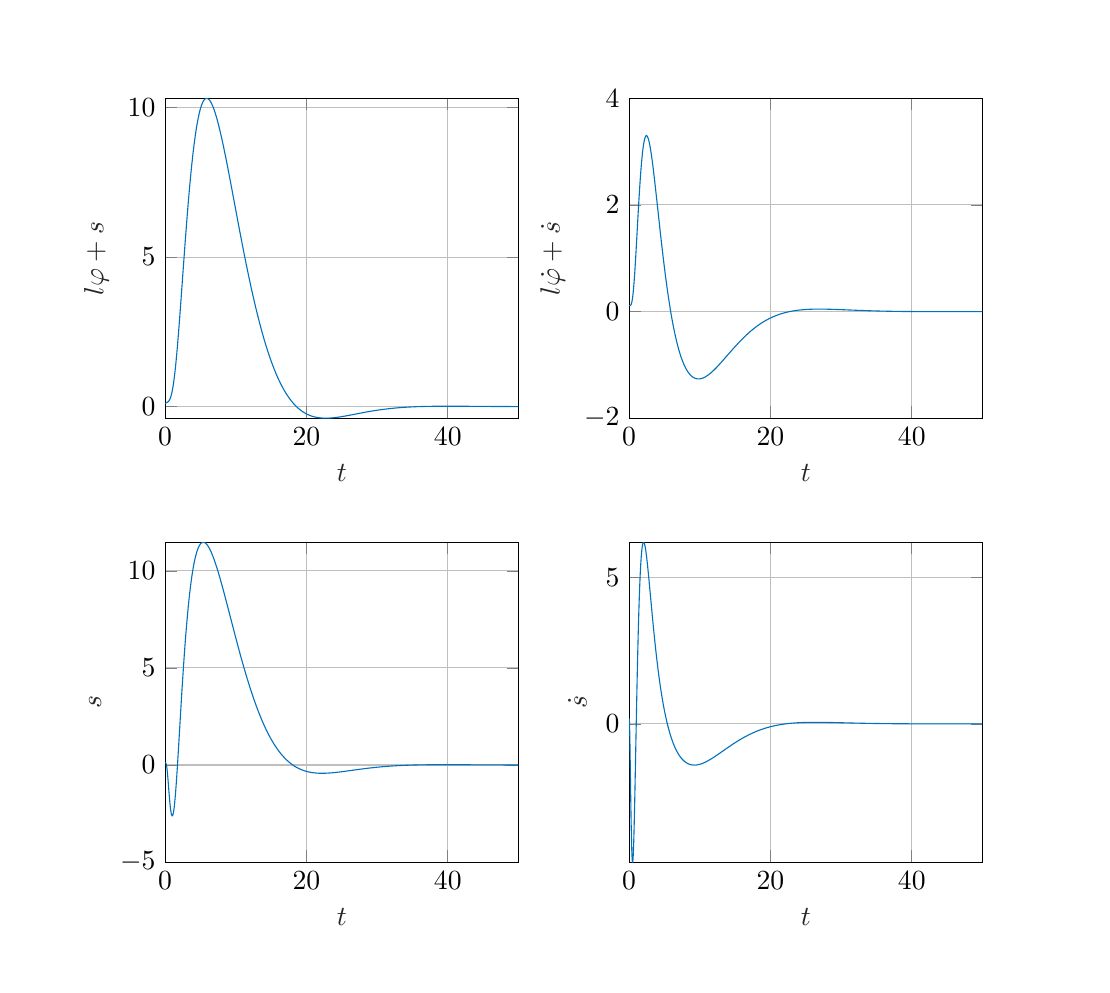
\begin{tikzpicture}

\begin{axis}[%
width=0.37\linewidth,
height=0.335\linewidth,
at={(0\linewidth,0.465\linewidth)},
scale only axis,
xmin=0,
xmax=50,
xlabel style={font=\color{white!15!black}},
xlabel={$t$},
ymin=-0.385740628910384,
ymax=10.3074861679762,
ylabel style={font=\color{white!15!black}},
ylabel={$l\varphi+s$},
axis background/.style={fill=white},
xmajorgrids,
ymajorgrids
]
\addplot [color=mycolor1, forget plot]
  table[row sep=crcr]{%
0	0.11\\
8.79073862042456e-05	0.110009669841462\\
0.000175814772408491	0.110019339740887\\
0.000263722158612737	0.11002900969828\\
0.000351629544816982	0.110038679713644\\
0.00079116647583821	0.110087030660192\\
0.00123070340685944	0.110135383056593\\
0.00167024033788067	0.110183736903164\\
0.00210977726890189	0.110232092200095\\
0.00430746192400803	0.110473890442751\\
0.00650514657911417	0.110715724900756\\
0.00870283123422031	0.110957595468479\\
0.0109005158893265	0.111199501996517\\
0.0218889391648572	0.112409583656717\\
0.0328773624403879	0.113620519856388\\
0.0438657857159186	0.114832276737612\\
0.0548542089914493	0.11604490391134\\
0.0685213066794778	0.117554544856612\\
0.0821884043675063	0.119066019840517\\
0.0958555020555349	0.12057992244495\\
0.109522599743563	0.122097253533159\\
0.12847096298975	0.124209236133374\\
0.147419326235936	0.126334979681081\\
0.166367689482122	0.128480545820681\\
0.185316052728308	0.130653921354441\\
0.204587811801823	0.132902813068071\\
0.223859570875339	0.135201835933442\\
0.243131329948854	0.137564273565367\\
0.262403089022369	0.140005192712766\\
0.285682928723189	0.143082246266111\\
0.308962768424008	0.146330276410843\\
0.332242608124828	0.149784309187837\\
0.355522447825647	0.153482008573047\\
0.378209341421843	0.157358071963529\\
0.400896235018038	0.161542435787463\\
0.423583128614234	0.166075503567024\\
0.446270022210429	0.170998701457864\\
0.469960064767812	0.176601832487699\\
0.493650107325195	0.182725903128863\\
0.517340149882577	0.18942058126148\\
0.54103019243996	0.196735347398883\\
0.565990025188309	0.205167278100199\\
0.590949857936658	0.214399913835619\\
0.615909690685007	0.224489802542358\\
0.640869523433356	0.235491884431105\\
0.675923470192424	0.252585102706613\\
0.710977416951492	0.271726074685739\\
0.74603136371056	0.293050090261753\\
0.781085310469628	0.316681450874903\\
0.822370774757663	0.34762728050242\\
0.863656239045698	0.382103828684637\\
0.904941703333733	0.420260903513027\\
0.946227167621768	0.462223472555035\\
0.997113834901503	0.519330907520892\\
1.04800050218124	0.582526454237202\\
1.09888716946097	0.651911211361154\\
1.14977383674071	0.727533914870178\\
1.21365213691803	0.831295245278344\\
1.27753043709535	0.94480324531103\\
1.34140873727267	1.06787492646632\\
1.40528703744999	1.20024009966552\\
1.48298426693461	1.37326842743966\\
1.56068149641922	1.55877111714748\\
1.63837872590384	1.75587263554265\\
1.71607595538845	1.96363090697407\\
1.80164391168615	2.20356735212331\\
1.88721186798386	2.45376110231822\\
1.97277982428156	2.71274207496895\\
2.05834778057926	2.97907860111239\\
2.15857068511346	3.29849195131199\\
2.25879358964765	3.62376036332286\\
2.35901649418185	3.95270355467331\\
2.45923939871604	4.28333317488031\\
2.58569761462329	4.70007011483439\\
2.71215583053053	5.11301162531539\\
2.83861404643778	5.51903428348168\\
2.96507226234503	5.9155222608935\\
3.12372831083571	6.39604788010709\\
3.2823843593264	6.8541927655213\\
3.44104040781708	7.28698078026536\\
3.59969645630776	7.69224020823973\\
3.76741679336023	8.08898805297143\\
3.9351371304127	8.45204873799955\\
4.10285746746516	8.78086745996553\\
4.27057780451763	9.07527839376313\\
4.44478734191165	9.34489207202349\\
4.61899687930568	9.57842514048394\\
4.7932064166997	9.77692156806641\\
4.96741595409372	9.94152945673219\\
5.15878806324502	10.0848589945764\\
5.35016017239631	10.1910025232129\\
5.5415322815476	10.2621256841289\\
5.7329043906989	10.3003319214593\\
5.93083095054909	10.3074861679762\\
6.12875751039928	10.2842123740989\\
6.32668407024947	10.2329143388948\\
6.52461063009966	10.1558671451108\\
6.77158122854326	10.026946847094\\
7.01855182698687	9.86558398641399\\
7.26552242543048	9.67573521690429\\
7.51249302387408	9.46102580018088\\
7.7654370208338	9.21889857429444\\
8.01838101779352	8.95771725869281\\
8.27132501475323	8.68064626236836\\
8.52426901171295	8.39059128182096\\
8.77721300867267	8.09022805046206\\
9.03015700563238	7.7819717299011\\
9.2831010025921	7.46802834441232\\
9.53604499955181	7.15045087806566\\
9.74177547486308	6.8907643571666\\
9.94750595017435	6.63075988191838\\
10.1532364254856	6.37124456451594\\
10.3589669007969	6.11299997764777\\
10.5244014313682	5.90674017789291\\
10.6898359619394	5.7020612909478\\
10.8552704925107	5.49926157310413\\
11.020705023082	5.29862611932373\\
11.191556731698	5.09396790573802\\
11.362408440314	4.8921419761135\\
11.53326014893	4.69337934894311\\
11.7041118575461	4.49789356201617\\
11.917893542033	4.25819472796911\\
12.13167522652	4.02424425797043\\
12.345456911007	3.79631998907399\\
12.5592385954939	3.57466564145666\\
12.8099837338305	3.32295144756153\\
13.0607288721671	3.08038100053255\\
13.3114740105037	2.84713696367898\\
13.5622191488403	2.6233681626765\\
13.7380231861397	2.47218003723036\\
13.9138272234392	2.32569642208172\\
14.0896312607386	2.18391689543947\\
14.2654352980381	2.04683773121905\\
14.4412393353375	1.91444407887507\\
14.617043372637	1.7867032369867\\
14.7928474099364	1.66357891346125\\
14.9686514472358	1.54503040090606\\
15.1829062921419	1.40667011136099\\
15.3971611370479	1.27492671826936\\
15.6114159819539	1.14968298582688\\
15.8256708268599	1.03081566819793\\
16.0669936171248	0.904401250082072\\
16.3083164073897	0.785690448208663\\
16.5496391976546	0.674459384267241\\
16.7909619879195	0.570486479079722\\
16.9627846650919	0.500753961288548\\
17.1346073422643	0.434490020583888\\
17.3064300194367	0.371604571565469\\
17.478252696609	0.312009536670744\\
17.6500753737814	0.25561525274431\\
17.8218980509538	0.202327537228028\\
17.9937207281262	0.152053853354706\\
18.1655434052985	0.104702749718704\\
18.3749424539623	0.0508147071108336\\
18.5843415026261	0.000962929526539785\\
18.7937405512899	-0.0450188432299755\\
19.0031395999537	-0.0872936435832616\\
19.2400002403302	-0.130847091529965\\
19.4768608807066	-0.170098635669342\\
19.7137215210831	-0.205277463907372\\
19.9505821614595	-0.236604280474114\\
20.1157167730934	-0.256281025823665\\
20.2808513847272	-0.274264931432229\\
20.445985996361	-0.29062733783387\\
20.6111206079948	-0.305437437199395\\
20.7762552196287	-0.318763199177562\\
20.9413898312625	-0.330672079860942\\
21.1065244428963	-0.341229551296427\\
21.2716590545302	-0.350499300841315\\
21.47148335905	-0.360083288245745\\
21.6713076635699	-0.367980352020305\\
21.8711319680897	-0.374294547487477\\
22.0709562726096	-0.379126184196012\\
22.2881773447399	-0.382809672978443\\
22.5053984168701	-0.384976038691747\\
22.7226194890004	-0.385740628910384\\
22.9398405611306	-0.385213610519187\\
23.1374037594104	-0.383701597674159\\
23.3349669576903	-0.381284818305043\\
23.5325301559701	-0.378036233425255\\
23.7300933542499	-0.374025425425752\\
23.9420913567563	-0.368949484991015\\
24.1540893592628	-0.363151066102737\\
24.3660873617693	-0.356704692115893\\
24.5780853642757	-0.349680763572348\\
24.8111637591628	-0.341371142469216\\
25.0442421540498	-0.332527773824827\\
25.2773205489368	-0.323229146922318\\
25.5103989438238	-0.313548175698087\\
25.738044879579	-0.303788853972415\\
25.9656908153342	-0.29378967050795\\
26.1933367510893	-0.283606065276627\\
26.4209826868445	-0.273288523769576\\
26.6189747710224	-0.264242499490898\\
26.8169668552002	-0.255160244801616\\
27.0149589393781	-0.246068787912357\\
27.2129510235559	-0.236992489395221\\
27.3928636978635	-0.228777191991347\\
27.572776372171	-0.220609612070152\\
27.7526890464786	-0.212504615498997\\
27.9326017207862	-0.204475654323715\\
28.1240751036456	-0.196028234564458\\
28.3155484865051	-0.187695141701894\\
28.5070218693645	-0.179489017488539\\
28.6984952522239	-0.171421123362507\\
28.9185839038819	-0.162331352763998\\
29.1386725555399	-0.153451538975714\\
29.3587612071978	-0.144793689264553\\
29.5788498588558	-0.136367866826191\\
29.810471466618	-0.127760356877232\\
30.0420930743803	-0.119427892498445\\
30.2737146821425	-0.111377233354588\\
30.5053362899048	-0.103612964374127\\
30.7127663292782	-0.0969053034570351\\
30.9201963686516	-0.0904321048885405\\
31.127626408025	-0.0841943604204382\\
31.3350564473984	-0.0781916717678677\\
31.513062527763	-0.0732271503396983\\
31.6910686081275	-0.0684346908584124\\
31.869074688492	-0.0638132604249519\\
32.0470807688565	-0.0593612897858558\\
32.2229346951254	-0.0551278055175708\\
32.3987886213943	-0.0510563109553935\\
32.5746425476633	-0.047144763266202\\
32.7504964739322	-0.0433908335244401\\
32.952902722929	-0.0392619653786288\\
33.1553089719258	-0.03533469411247\\
33.3577152209226	-0.0316047779778195\\
33.5601214699194	-0.0280676771861901\\
33.7895628111794	-0.0242853113905493\\
34.0190041524394	-0.020737657261604\\
34.2484454936994	-0.0174174398324976\\
34.4778868349595	-0.0143170419556049\\
34.6980781577542	-0.0115411325930093\\
34.9182694805489	-0.00895388981023238\\
35.1384608033437	-0.006548480766318\\
35.3586521261384	-0.00431776824557383\\
35.5426690376131	-0.00258238310732932\\
35.7266859490878	-0.000960196749684772\\
35.9107028605625	0.00055278809810398\\
36.0947197720372	0.00196067350211256\\
36.2592933635184	0.00313407255392982\\
36.4238669549997	0.0042293709179304\\
36.5884405464809	0.00524934828744442\\
36.7530141379621	0.00619678204211952\\
36.9331593548863	0.00715392569543077\\
37.1133045718104	0.00803090707134392\\
37.2934497887345	0.00883117574816994\\
37.4735950056586	0.00955813177916957\\
37.6863439315541	0.0103267838623514\\
37.8990928574495	0.0110031600036951\\
38.1118417833449	0.0115924672306232\\
38.3245907092404	0.0120997837449591\\
38.5470546817302	0.0125479248284377\\
38.76951865422	0.0129172223083039\\
38.9919826267098	0.0132129268154339\\
39.2144465991997	0.0134401342571737\\
39.3995985395001	0.0135805408416413\\
39.5847504798006	0.013679589534072\\
39.7699024201011	0.0137398999716302\\
39.9550543604016	0.0137640185219244\\
40.1152696182597	0.0137575722022102\\
40.2754848761177	0.0137273809977366\\
40.4357001339757	0.0136749223734729\\
40.5959153918338	0.0136016278769269\\
40.7820443998639	0.013492140439348\\
40.9681734078941	0.0133584702986365\\
41.1543024159243	0.0132026095199662\\
41.3404314239545	0.0130264672443206\\
41.5929339086321	0.0127583448831723\\
41.8454363933096	0.0124605417517996\\
42.0979388779872	0.0121370869609577\\
42.3504413626648	0.0117917587986343\\
42.5685208809169	0.0114786166183167\\
42.786600399169	0.0111538875444388\\
43.0046799174212	0.0108195460222993\\
43.2227594356733	0.0104774548270974\\
43.4408389539255	0.0101293518507544\\
43.6589184721776	0.00977682151566989\\
43.8769979904298	0.00942134709656472\\
44.0950775086819	0.00906432447666621\\
44.309144596713	0.00871361089765547\\
44.523211684744	0.00836372901069185\\
44.737278772775	0.00801568824881929\\
44.951345860806	0.00767043967641014\\
45.1523310456906	0.00734960394347673\\
45.3533162305752	0.00703260659594777\\
45.5543014154598	0.00672002202114361\\
45.7552866003444	0.00641239188245449\\
45.9480882864836	0.00612239375796517\\
46.1408899726229	0.00583775584536243\\
46.3336916587622	0.00555880731512575\\
46.5264933449014	0.00528585401803971\\
46.7242617166483	0.00501237795126134\\
46.9220300883951	0.00474571801276873\\
47.119798460142	0.00448607653272271\\
47.3175668318888	0.00423363430013681\\
47.5273591292533	0.0039738775624703\\
47.7371514266178	0.00372250482067892\\
47.9469437239823	0.00347960766091355\\
48.1567360213468	0.00324525897313335\\
48.3704606432172	0.00301535104541871\\
48.5841852650876	0.00279434677767675\\
48.797909886958	0.00258221791607645\\
49.0116345088284	0.00237892731392611\\
49.2145435316358	0.00219404663815689\\
49.4174525544431	0.00201698112973702\\
49.6203615772505	0.00184763120908624\\
49.8232706000578	0.00168589703731619\\
49.8674529500433	0.00165167949522511\\
49.9116353000289	0.00161781570818118\\
49.9558176500145	0.00158430432436337\\
50	0.00155114396574625\\
};
\end{axis}

\begin{axis}[%
width=0.37\linewidth,
height=0.335\linewidth,
at={(0.486\linewidth,0.465\linewidth)},
scale only axis,
xmin=0,
xmax=50,
xlabel style={font=\color{white!15!black}},
xlabel={$t$},
ymin=-2,
ymax=4,
ylabel style={font=\color{white!15!black}},
ylabel={$l\dot\varphi+\dot s$},
axis background/.style={fill=white},
xmajorgrids,
ymajorgrids
]
\addplot [color=mycolor1, forget plot]
  table[row sep=crcr]{%
0	0.11\\
8.79073862042456e-05	0.110000659333943\\
0.000175814772408491	0.110001318723255\\
0.000263722158612737	0.110001978165361\\
0.000351629544816982	0.110002637657698\\
0.00079116647583821	0.110005935784176\\
0.00123070340685944	0.110009234790331\\
0.00167024033788067	0.110012534371831\\
0.00210977726890189	0.110015834233071\\
0.00430746192400803	0.110032327951597\\
0.00650514657911417	0.110048789322916\\
0.00870283123422031	0.11006519105938\\
0.0109005158893265	0.110081510963171\\
0.0218889391648572	0.110161294475075\\
0.0328773624403879	0.110238586782396\\
0.0438657857159186	0.110315942041975\\
0.0548542089914493	0.110397979197129\\
0.0685213066794778	0.110516806812602\\
0.0821884043675063	0.110671624239462\\
0.0958555020555349	0.110884082250372\\
0.109522599743563	0.111178013518437\\
0.12847096298975	0.11176907766902\\
0.147419326235936	0.112647265477532\\
0.166367689482122	0.113896512037033\\
0.185316052728308	0.115599630388735\\
0.204587811801823	0.117883853559799\\
0.223859570875339	0.120816844198897\\
0.243131329948854	0.124487176379115\\
0.262403089022369	0.128977740372278\\
0.285682928723189	0.135607642811938\\
0.308962768424008	0.143683199139226\\
0.332242608124828	0.153325294751356\\
0.355522447825647	0.164638025046351\\
0.378209341421843	0.177356492358662\\
0.400896235018038	0.191822409441801\\
0.423583128614234	0.208096187699773\\
0.446270022210429	0.226224330873567\\
0.469960064767812	0.247170065703985\\
0.493650107325195	0.270200864485819\\
0.517340149882577	0.295328495575861\\
0.54103019243996	0.322551417289897\\
0.565990025188309	0.353484924044358\\
0.590949857936658	0.386698649543975\\
0.615909690685007	0.422149335021509\\
0.640869523433356	0.459782325762639\\
0.675923470192424	0.516193390981895\\
0.710977416951492	0.576561674775774\\
0.74603136371056	0.640639400820121\\
0.781085310469628	0.708157629224922\\
0.822370774757663	0.791698632056418\\
0.863656239045698	0.879096919003788\\
0.904941703333733	0.96982233072026\\
0.946227167621768	1.06334669188516\\
0.997113834901503	1.1816902062785\\
1.04800050218124	1.30246576370351\\
1.09888716946097	1.42469133157657\\
1.14977383674071	1.54745507157211\\
1.21365213691803	1.70101230472664\\
1.27753043709535	1.85242150274796\\
1.34140873727267	2.00021169555954\\
1.40528703744999	2.14313868200467\\
1.48298426693461	2.30888711417264\\
1.56068149641922	2.46414848400914\\
1.63837872590384	2.60759271347899\\
1.71607595538845	2.73826992986203\\
1.80164391168615	2.86661960600497\\
1.88721186798386	2.97812607100145\\
1.97277982428156	3.07259378679558\\
2.05834778057926	3.1500890633755\\
2.15857068511346	3.2196641415656\\
2.25879358964765	3.26725971356619\\
2.35901649418185	3.29403310759953\\
2.45923939871604	3.30122176837566\\
2.58569761462329	3.28441968210673\\
2.71215583053053	3.24181687675641\\
2.83861404643778	3.17663403669862\\
2.96507226234503	3.09173737757429\\
3.12372831083571	2.96151226482369\\
3.2823843593264	2.81031631836171\\
3.44104040781708	2.64322273287995\\
3.59969645630776	2.46427626387522\\
3.76741679336023	2.26616278563639\\
3.9351371304127	2.06286961459491\\
4.10285746746516	1.85763444114065\\
4.27057780451763	1.65304347769309\\
4.44478734191165	1.44349900424009\\
4.61899687930568	1.23888192460827\\
4.7932064166997	1.04065214207189\\
4.96741595409372	0.84996697273886\\
5.15878806324502	0.650218339499579\\
5.35016017239631	0.461270673998432\\
5.5415322815476	0.283517177584599\\
5.7329043906989	0.11722384387073\\
5.93083095054909	-0.042625554421901\\
6.12875751039928	-0.190354760182531\\
6.32668407024947	-0.326258926326407\\
6.52461063009966	-0.450649934530817\\
6.77158122854326	-0.590286603380687\\
7.01855182698687	-0.713585960930837\\
7.26552242543048	-0.821563271973498\\
7.51249302387408	-0.915146050867258\\
7.7654370208338	-0.997061934535082\\
8.01838101779352	-1.06597016465291\\
8.27132501475323	-1.12289116328116\\
8.52426901171295	-1.16880846683679\\
8.77721300867267	-1.20469139468282\\
9.03015700563238	-1.23133487023953\\
9.2831010025921	-1.24952197499749\\
9.53604499955181	-1.26015419474105\\
9.74177547486308	-1.26382596928372\\
9.94750595017435	-1.26328516140358\\
10.1532364254856	-1.25883744019057\\
10.3589669007969	-1.25093320208768\\
10.5244014313682	-1.24234217140001\\
10.6898359619394	-1.23183841236357\\
10.8552704925107	-1.2195615951879\\
11.020705023082	-1.2056828749022\\
11.191556731698	-1.18983128396243\\
11.362408440314	-1.17254607339461\\
11.53326014893	-1.15395742536737\\
11.7041118575461	-1.13420321802866\\
11.917893542033	-1.10803968878217\\
12.13167522652	-1.0804530323384\\
12.345456911007	-1.05164391005264\\
12.5592385954939	-1.0218212877417\\
12.8099837338305	-0.985820740107646\\
13.0607288721671	-0.948918582493029\\
13.3114740105037	-0.911337844919083\\
13.5622191488403	-0.87335704843376\\
13.7380231861397	-0.846624651681917\\
13.9138272234392	-0.819843001125056\\
14.0896312607386	-0.793066604718209\\
14.2654352980381	-0.766370631645681\\
14.4412393353375	-0.739819948169035\\
14.617043372637	-0.713443905663614\\
14.7928474099364	-0.687284789686904\\
14.9686514472358	-0.661391409503797\\
15.1829062921419	-0.630257323767386\\
15.3971611370479	-0.59963062661712\\
15.6114159819539	-0.569562426352491\\
15.8256708268599	-0.540112382177315\\
16.0669936171248	-0.507751483042986\\
16.3083164073897	-0.476270175176885\\
16.5496391976546	-0.445701619492056\\
16.7909619879195	-0.416111178903881\\
16.9627846650919	-0.395668479020528\\
17.1346073422643	-0.375736614822637\\
17.3064300194367	-0.356320116622045\\
17.478252696609	-0.337433253951664\\
17.6500753737814	-0.319085882798781\\
17.8218980509538	-0.301272418614332\\
17.9937207281262	-0.283993441009284\\
18.1655434052985	-0.267252418216984\\
18.3749424539623	-0.247579747642857\\
18.5843415026261	-0.228699376933743\\
18.7937405512899	-0.210604176636462\\
19.0031395999537	-0.193290521655433\\
19.2400002403302	-0.174642031353325\\
19.4768608807066	-0.156961671835902\\
19.7137215210831	-0.140227531635814\\
19.9505821614595	-0.124428684487071\\
20.1157167730934	-0.113959753414948\\
20.2808513847272	-0.103924311598128\\
20.445985996361	-0.0943135755172177\\
20.6111206079948	-0.0851212999777211\\
20.7762552196287	-0.0763401914057485\\
20.9413898312625	-0.0679592734017073\\
21.1065244428963	-0.0599692063592302\\
21.2716590545302	-0.0523613521159627\\
21.47148335905	-0.0436535602698337\\
21.6713076635699	-0.0354742696831759\\
21.8711319680897	-0.0278060783860565\\
22.0709562726096	-0.0206324121179313\\
22.2881773447399	-0.0133756891485554\\
22.5053984168701	-0.00666015884024623\\
22.7226194890004	-0.000463261800534454\\
22.9398405611306	0.00523611987743955\\
23.1374037594104	0.0100054585887968\\
23.3349669576903	0.0143980773134875\\
23.5325301559701	0.0184303092139906\\
23.7300933542499	0.0221173281395633\\
23.9420913567563	0.0257068800051579\\
24.1540893592628	0.0289362623347033\\
24.3660873617693	0.0318243284051115\\
24.5780853642757	0.0343883885304959\\
24.8111637591628	0.0368534924190907\\
25.0442421540498	0.0389719418244168\\
25.2773205489368	0.0407665899321775\\
25.5103989438238	0.0422571666545201\\
25.738044879579	0.0434374240905786\\
25.9656908153342	0.0443674519277444\\
26.1933367510893	0.0450664048961288\\
26.4209826868445	0.045548451078986\\
26.6189747710224	0.0458021093751552\\
26.8169668552002	0.0459162064185697\\
27.0149589393781	0.045901641574011\\
27.2129510235559	0.0457657996158383\\
27.3928636978635	0.045543597226443\\
27.572776372171	0.045236451910619\\
27.7526890464786	0.0448510964095909\\
27.9326017207862	0.0443927196802066\\
28.1240751036456	0.0438305383160617\\
28.3155484865051	0.0431995834536147\\
28.5070218693645	0.0425065827084434\\
28.6984952522239	0.0417570851303865\\
28.9185839038819	0.0408326875198786\\
29.1386725555399	0.0398503797906855\\
29.3587612071978	0.0388185213046493\\
29.5788498588558	0.0377436108524113\\
29.810471466618	0.0365723624945714\\
30.0420930743803	0.0353697724769542\\
30.2737146821425	0.0341437550175782\\
30.5053362899048	0.0328988704765669\\
30.7127663292782	0.0317713958263437\\
30.9201963686516	0.0306389360725995\\
31.127626408025	0.0295060219691801\\
31.3350564473984	0.0283741016169454\\
31.513062527763	0.0274048170919651\\
31.6910686081275	0.0264412321631016\\
31.869074688492	0.0254853301708581\\
32.0470807688565	0.0245379141322406\\
32.2229346951254	0.0236112055894791\\
32.3987886213943	0.022695795281867\\
32.5746425476633	0.0217929785083639\\
32.7504964739322	0.0209035344144272\\
32.952902722929	0.0198973396246294\\
33.1553089719258	0.0189117024658582\\
33.3577152209226	0.0179479358939787\\
33.5601214699194	0.0170067915891696\\
33.7895628111794	0.0159680638885486\\
34.0190041524394	0.0149609639344945\\
34.2484454936994	0.0139866392837235\\
34.4778868349595	0.0130452196572284\\
34.6980781577542	0.0121726188293098\\
34.9182694805489	0.0113316114361015\\
35.1384608033437	0.0105227497266837\\
35.3586521261384	0.00974524971059352\\
35.5426690376131	0.00911901725059937\\
35.7266859490878	0.0085149563793703\\
35.9107028605625	0.00793309206705699\\
36.0947197720372	0.00737285081809742\\
36.2592933635184	0.00688972959633541\\
36.4238669549997	0.0064237000088322\\
36.5884405464809	0.0059746026803546\\
36.7530141379621	0.00554212345882296\\
36.9331593548863	0.00508742712841091\\
37.1133045718104	0.00465209167526076\\
37.2934497887345	0.00423579611251417\\
37.4735950056586	0.00383812953636149\\
37.6863439315541	0.00339191407613638\\
37.8990928574495	0.0029705499669435\\
38.1118417833449	0.00257339455125707\\
38.3245907092404	0.00219969000365675\\
38.5470546817302	0.0018331609136102\\
38.76951865422	0.0014907311960593\\
38.9919826267098	0.00117160711651183\\
39.2144465991997	0.000874833177552347\\
39.3995985395001	0.000644199516263571\\
39.5847504798006	0.000428012202576749\\
39.7699024201011	0.000225798372362457\\
39.9550543604016	3.70132684805814e-05\\
40.1152696182597	-0.00011591303674902\\
40.2754848761177	-0.000259448367330582\\
40.4357001339757	-0.000393901467683784\\
40.5959153918338	-0.000519593019185488\\
40.7820443998639	-0.000655026728861209\\
40.9681734078941	-0.000779516413926163\\
41.1543024159243	-0.000893525531374672\\
41.3404314239545	-0.000997519821428015\\
41.5929339086321	-0.00112340815766823\\
41.8454363933096	-0.0012327792070405\\
42.0979388779872	-0.00132668800106566\\
42.3504413626648	-0.00140619655636307\\
42.5685208809169	-0.00146407082183207\\
42.786600399169	-0.00151254979425463\\
43.0046799174212	-0.00155221942293813\\
43.2227594356733	-0.00158370225209542\\
43.4408389539255	-0.00160759941406542\\
43.6589184721776	-0.00162438010334764\\
43.8769979904298	-0.00163454085769515\\
44.0950775086819	-0.0016386374870212\\
44.309144596713	-0.0016372754292166\\
44.523211684744	-0.00163092326518655\\
44.737278772775	-0.00161996647328339\\
44.951345860806	-0.00160487093811501\\
45.1523310456906	-0.00158732048273196\\
45.3533162305752	-0.00156671142756745\\
45.5543014154598	-0.00154330440929235\\
45.7552866003444	-0.00151742800010793\\
45.9480882864836	-0.00149056426299472\\
46.1408899726229	-0.00146185039782393\\
46.3336916587622	-0.00143147638259783\\
46.5264933449014	-0.00139967427451853\\
46.7242617166483	-0.00136579179390351\\
46.9220300883951	-0.00133076612156609\\
47.119798460142	-0.00129476207808591\\
47.3175668318888	-0.00125797532204287\\
47.5273591292533	-0.00121829764825238\\
47.7371514266178	-0.00117806824534054\\
47.9469437239823	-0.00113743567680218\\
48.1567360213468	-0.00109658377391626\\
48.3704606432172	-0.00105491619664672\\
48.5841852650876	-0.00101327803630552\\
48.797909886958	-0.000971777870122188\\
49.0116345088284	-0.000930571668020907\\
49.2145435316358	-0.000891850360391655\\
49.4174525544431	-0.000853546437003687\\
49.6203615772505	-0.000815720134397001\\
49.8232706000578	-0.000778475198395283\\
49.8674529500433	-0.000770453413939938\\
49.9116353000289	-0.000762461884213087\\
49.9558176500145	-0.000754501254142733\\
50	-0.000746572147485799\\
};
\end{axis}

\begin{axis}[%
width=0.37\linewidth,
height=0.335\linewidth,
at={(0\linewidth,0\linewidth)},
scale only axis,
xmin=0,
xmax=50,
xlabel style={font=\color{white!15!black}},
xlabel={$t$},
ymin=-5,
ymax=11.4687862108246,
ylabel style={font=\color{white!15!black}},
ylabel={$s$},
axis background/.style={fill=white},
xmajorgrids,
ymajorgrids
]
\addplot [color=mycolor1, forget plot]
  table[row sep=crcr]{%
0	0.1\\
8.79073862042456e-05	0.100008810427164\\
0.000175814772408491	0.100017660088036\\
0.000263722158612737	0.100026548767691\\
0.000351629544816982	0.100035476251388\\
0.00079116647583821	0.100080688227649\\
0.00123070340685944	0.100126838201921\\
0.00167024033788067	0.100173899542389\\
0.00210977726890189	0.100221845733454\\
0.00430746192400803	0.100473929116387\\
0.00650514657911417	0.100744223078994\\
0.00870283123422031	0.101029542537297\\
0.0109005158893265	0.101326771863396\\
0.0218889391648572	0.102885955562783\\
0.0328773624403879	0.104315076217018\\
0.0438657857159186	0.105299189402203\\
0.0548542089914493	0.105557024056043\\
0.0685213066794778	0.104493206987666\\
0.0821884043675063	0.10152768761882\\
0.0958555020555349	0.0963288485218497\\
0.109522599743563	0.0886195194934489\\
0.12847096298975	0.073367887498625\\
0.147419326235936	0.0524763153097657\\
0.166367689482122	0.0257050699314875\\
0.185316052728308	-0.00708026753782255\\
0.204587811801823	-0.0466082794707081\\
0.223859570875339	-0.09223153423228\\
0.243131329948854	-0.143737925840377\\
0.262403089022369	-0.200865890280514\\
0.285682928723189	-0.276914355381936\\
0.308962768424008	-0.359977166264376\\
0.332242608124828	-0.449278195000108\\
0.355522447825647	-0.544034169038251\\
0.378209341421843	-0.640845303963098\\
0.400896235018038	-0.741240736962277\\
0.423583128614234	-0.844419278889586\\
0.446270022210429	-0.949610128311382\\
0.469960064767812	-1.06078374589513\\
0.493650107325195	-1.17247033195233\\
0.517340149882577	-1.28385677129146\\
0.54103019243996	-1.39418486320989\\
0.565990025188309	-1.5084959067982\\
0.590949857936658	-1.62004270982099\\
0.615909690685007	-1.7280953548289\\
0.640869523433356	-1.83199398580773\\
0.675923470192424	-1.96976434514306\\
0.710977416951492	-2.09669477464762\\
0.74603136371056	-2.21154199643898\\
0.781085310469628	-2.31330455474458\\
0.822370774757663	-2.41530153337777\\
0.863656239045698	-2.49707422179932\\
0.904941703333733	-2.55799168833392\\
0.946227167621768	-2.59771622904331\\
0.997113834901503	-2.6174078621839\\
1.04800050218124	-2.60519732648459\\
1.09888716946097	-2.56191786120962\\
1.14977383674071	-2.48867012112978\\
1.21365213691803	-2.35638039986818\\
1.27753043709535	-2.18249271841789\\
1.34140873727267	-1.97076377474886\\
1.40528703744999	-1.72485008764292\\
1.48298426693461	-1.38498503459432\\
1.56068149641922	-1.0073489497098\\
1.63837872590384	-0.598856231093813\\
1.71607595538845	-0.165525010190392\\
1.80164391168615	0.333778383975582\\
1.88721186798386	0.84897244297131\\
1.97277982428156	1.37362766693597\\
2.05834778057926	1.90240418072055\\
2.15857068511346	2.52077861905649\\
2.25879358964765	3.13185215921169\\
2.35901649418185	3.73036855660698\\
2.45923939871604	4.31221805797335\\
2.58569761462329	5.01755369316464\\
2.71215583053053	5.6866389648073\\
2.83861404643778	6.31659473314072\\
2.96507226234503	6.90543322295752\\
3.12372831083571	7.58434134662116\\
3.2823843593264	8.19785401630356\\
3.44104040781708	8.74808787333855\\
3.59969645630776	9.23672817854608\\
3.76741679336023	9.68886996733121\\
3.9351371304127	10.0796061119191\\
4.10285746746516	10.4133030426973\\
4.27057780451763	10.693604556691\\
4.44478734191165	10.9321088474331\\
4.61899687930568	11.1216329406029\\
4.7932064166997	11.2662937466824\\
4.96741595409372	11.3697156152197\\
5.15878806324502	11.4398462734025\\
5.35016017239631	11.4687862108246\\
5.5415322815476	11.4605152080447\\
5.7329043906989	11.4186167155692\\
5.93083095054909	11.3434228163705\\
6.12875751039928	11.2392039872915\\
6.32668407024947	11.109044700385\\
6.52461063009966	10.9557771189527\\
6.77158122854326	10.7360670353958\\
7.01855182698687	10.4890058765156\\
7.26552242543048	10.2187194889823\\
7.51249302387408	9.92895057724594\\
7.7654370208338	9.61547428459771\\
8.01838101779352	9.28844627371559\\
8.27132501475323	8.9508813660672\\
8.52426901171295	8.60531117012505\\
8.77721300867267	8.25387121069458\\
9.03015700563238	7.89926510187776\\
9.2831010025921	7.54370500905902\\
9.53604499955181	7.18832420790737\\
9.74177547486308	6.90005214517549\\
9.94750595017435	6.61407055254978\\
10.1532364254856	6.33130300915016\\
10.3589669007969	6.05177953831573\\
10.5244014313682	5.82944613886418\\
10.6898359619394	5.61002467406885\\
10.8552704925107	5.39379878908593\\
11.020705023082	5.18083733678513\\
11.191556731698	4.96443806537848\\
11.362408440314	4.75197731539758\\
11.53326014893	4.54364921969142\\
11.7041118575461	4.33955661370553\\
11.917893542033	4.09029439080478\\
12.13167522652	3.84814940139267\\
12.345456911007	3.61334306503181\\
12.5592385954939	3.38595199489387\\
12.8099837338305	3.12871276826226\\
13.0607288721671	2.88207517021189\\
13.3114740105037	2.64622280302221\\
13.5622191488403	2.42090966590647\\
13.7380231861397	2.26908518158497\\
13.9138272234392	2.12249956950955\\
14.0896312607386	1.98115105010984\\
14.2654352980381	1.84490425944157\\
14.4412393353375	1.71364753393567\\
14.617043372637	1.58742016532753\\
14.7928474099364	1.4661710741852\\
14.9686514472358	1.34979323419153\\
15.1829062921419	1.2143965452029\\
15.3971611370479	1.08600351329069\\
15.6114159819539	0.964478518320437\\
15.8256708268599	0.849605035499474\\
16.0669936171248	0.72789101351148\\
16.3083164073897	0.61420155409339\\
16.5496391976546	0.508329511798489\\
16.7909619879195	0.40986319180052\\
16.9627846650919	0.34405195281734\\
17.1346073422643	0.281799580093892\\
17.3064300194367	0.223017299236877\\
17.478252696609	0.167559425696853\\
17.6500753737814	0.115295230411741\\
17.8218980509538	0.0661645675664615\\
17.9937207281262	0.0200702078624903\\
18.1655434052985	-0.0231047273353207\\
18.3749424539623	-0.0719373636244031\\
18.5843415026261	-0.116754579085929\\
18.7937405512899	-0.157727538593664\\
19.0031395999537	-0.195050991458449\\
19.2400002403302	-0.233114418549843\\
19.4768608807066	-0.266954944906678\\
19.7137215210831	-0.296794161124767\\
19.9505821614595	-0.322911550363719\\
20.1157167730934	-0.339059158716049\\
20.2808513847272	-0.353570557961813\\
20.445985996361	-0.366516502922317\\
20.6111206079948	-0.377980213706975\\
20.7762552196287	-0.388039198100549\\
20.9413898312625	-0.396752022231401\\
21.1065244428963	-0.404184676096063\\
21.2716590545302	-0.410405594231926\\
21.47148335905	-0.416406802198266\\
21.6713076635699	-0.420833417374166\\
21.8711319680897	-0.423789160126801\\
22.0709562726096	-0.425378292826815\\
22.2881773447399	-0.425672260420999\\
22.5053984168701	-0.424583666951254\\
22.7226194890004	-0.42222538290091\\
22.9398405611306	-0.418711299452524\\
23.1374037594104	-0.414602703074103\\
23.3349669576903	-0.409696931625045\\
23.5325301559701	-0.404064210738102\\
23.7300933542499	-0.397776006439463\\
23.9420913567563	-0.390376333636708\\
24.1540893592628	-0.382370308007744\\
24.3660873617693	-0.373828256331246\\
24.5780853642757	-0.36482204785122\\
24.8111637591628	-0.354465947002183\\
25.0442421540498	-0.343701650998534\\
25.2773205489368	-0.33259993062415\\
25.5103989438238	-0.321238502947732\\
25.738044879579	-0.309962154213112\\
25.9656908153342	-0.298546955202503\\
26.1933367510893	-0.287037703042056\\
26.4209826868445	-0.275497034230034\\
26.6189747710224	-0.265478567496037\\
26.8169668552002	-0.255487343533709\\
27.0149589393781	-0.24554320782302\\
27.2129510235559	-0.235679995366708\\
27.3928636978635	-0.226811895265262\\
27.572776372171	-0.218037106236449\\
27.7526890464786	-0.209366892476312\\
27.9326017207862	-0.200818001044433\\
28.1240751036456	-0.191868978725949\\
28.3155484865051	-0.18307893381163\\
28.5070218693645	-0.174457111096952\\
28.6984952522239	-0.166016083483067\\
28.9185839038819	-0.156551173593542\\
29.1386725555399	-0.147343959581937\\
29.3587612071978	-0.138401347902945\\
29.5788498588558	-0.129735779823398\\
29.810471466618	-0.120928014881553\\
30.0420930743803	-0.11243379411054\\
30.2737146821425	-0.104252429457314\\
30.5053362899048	-0.0963963870816863\\
30.7127663292782	-0.0896457865047624\\
30.9201963686516	-0.0831501459449921\\
31.127626408025	-0.0769044060742312\\
31.3350564473984	-0.0709171777230603\\
31.513062527763	-0.0659894925754819\\
31.6910686081275	-0.0612448628398861\\
31.869074688492	-0.0566799038792383\\
32.0470807688565	-0.0522963590568068\\
32.2229346951254	-0.048144119217876\\
32.3987886213943	-0.0441623557078299\\
32.5746425476633	-0.0403476904738114\\
32.7504964739322	-0.0366987105327199\\
32.952902722929	-0.0327012532091645\\
33.1553089719258	-0.0289131033060596\\
33.3577152209226	-0.0253283838828774\\
33.5601214699194	-0.0219432092922456\\
33.7895628111794	-0.0183420899339754\\
34.0190041524394	-0.0149804027631679\\
34.2484454936994	-0.0118484199556776\\
34.4778868349595	-0.00894063025998276\\
34.6980781577542	-0.00635587593619502\\
34.9182694805489	-0.00395962731544464\\
35.1384608033437	-0.00174242130874649\\
35.3586521261384	0.000298911163282949\\
35.5426690376131	0.00187287560964524\\
35.7266859490878	0.00333550653343485\\
35.9107028605625	0.00469187555331066\\
36.0947197720372	0.00594415157480674\\
36.2592933635184	0.00697821383728185\\
36.4238669549997	0.00793601486007714\\
36.5884405464809	0.00882064818080057\\
36.7530141379621	0.00963446262267247\\
36.9331593548863	0.0104470410379849\\
37.1133045718104	0.0111820480533713\\
37.2934497887345	0.0118431789535752\\
37.4735950056586	0.0124336750892738\\
37.6863439315541	0.0130444687266283\\
37.8990928574495	0.013567255228058\\
38.1118417833449	0.0140075351509237\\
38.3245907092404	0.0143701313701682\\
38.5470546817302	0.0146712513808796\\
38.76951865422	0.0148987384026759\\
38.9919826267098	0.0150581473602309\\
39.2144465991997	0.0151540166165469\\
39.3995985395001	0.0151885580741842\\
39.5847504798006	0.0151854393434166\\
39.7699024201011	0.0151473748906704\\
39.9550543604016	0.0150766003174371\\
40.1152696182597	0.0149906775882476\\
40.2754848761177	0.0148836621845563\\
40.4357001339757	0.0147570250673291\\
40.5959153918338	0.0146121072093854\\
40.7820443998639	0.0144225268087695\\
40.9681734078941	0.0142121493823439\\
41.1543024159243	0.0139829288162229\\
41.3404314239545	0.0137366749649559\\
41.5929339086321	0.0133784367091666\\
41.8454363933096	0.0129962858865273\\
42.0979388779872	0.0125941476247687\\
42.3504413626648	0.012175460304731\\
42.5685208809169	0.0118029592560577\\
42.786600399169	0.0114226998626515\\
43.0046799174212	0.0110366203451136\\
43.2227594356733	0.0106462378659904\\
43.4408389539255	0.0102529477401302\\
43.6589184721776	0.00985858790175973\\
43.8769979904298	0.00946463669928093\\
44.0950775086819	0.00907205654820047\\
44.309144596713	0.00868887548382791\\
44.523211684744	0.00830931171998343\\
44.737278772775	0.00793440745804667\\
44.951345860806	0.00756461920349786\\
45.1523310456906	0.00722246987882283\\
45.3533162305752	0.00688622214140657\\
45.5543014154598	0.00655647853622994\\
45.7552866003444	0.00623337638798826\\
45.9480882864836	0.0059298159899554\\
46.1408899726229	0.00563316242407415\\
46.3336916587622	0.00534374554389488\\
46.5264933449014	0.00506159399933284\\
46.7242617166483	0.00477976572715919\\
46.9220300883951	0.00450604921123499\\
47.119798460142	0.00424063489946584\\
47.3175668318888	0.00398347509978867\\
47.5273591292533	0.00371964504233061\\
47.7371514266178	0.00346533734654172\\
47.9469437239823	0.00322063894955967\\
48.1567360213468	0.00298537351159589\\
48.3704606432172	0.00275520307873538\\
48.5841852650876	0.00253483718812109\\
48.797909886958	0.0023242679530839\\
49.0116345088284	0.00212317526843194\\
49.2145435316358	0.00194074538349339\\
49.4174525544431	0.00176672666250474\\
49.6203615772505	0.00160104640096446\\
49.8232706000578	0.0014433660551947\\
49.8674529500433	0.0014100515139424\\
49.9116353000289	0.00137711067763537\\
49.9558176500145	0.00134454137372728\\
50	0.00131234144764839\\
};
\end{axis}

\begin{axis}[%
width=0.37\linewidth,
height=0.335\linewidth,
at={(0.486\linewidth,0\linewidth)},
scale only axis,
xmin=0,
xmax=50,
xlabel style={font=\color{white!15!black}},
xlabel={$t$},
ymin=-4.7136980255994,
ymax=6.18607279397737,
ylabel style={font=\color{white!15!black}},
ylabel={$\dot s$},
axis background/.style={fill=white},
xmajorgrids,
ymajorgrids
]
\addplot [color=mycolor1, forget plot]
  table[row sep=crcr]{%
0	0.1\\
8.79073862042456e-05	0.100447530477777\\
0.000175814772408491	0.100892614965901\\
0.000263722158612737	0.101335255599781\\
0.000351629544816982	0.101775454513601\\
0.00079116647583821	0.103939897893364\\
0.00123070340685944	0.106043617696406\\
0.00167024033788067	0.108086879322402\\
0.00210977726890189	0.110069947412184\\
0.00430746192400803	0.119091596389605\\
0.00650514657911417	0.126647667662553\\
0.00870283123422031	0.132770395076312\\
0.0109005158893265	0.137491555343731\\
0.0218889391648572	0.141161649788693\\
0.0328773624403879	0.114298477035362\\
0.0438657857159186	0.0603798589697716\\
0.0548542089914493	-0.0173494674726576\\
0.0685213066794778	-0.142724989333384\\
0.0821884043675063	-0.295029492135076\\
0.0958555020555349	-0.469475686501484\\
0.109522599743563	-0.661687833234546\\
0.12847096298975	-0.950209006030494\\
0.147419326235936	-1.25618578385107\\
0.166367689482122	-1.5717302818601\\
0.185316052728308	-1.88991844977053\\
0.204587811801823	-2.21017783801252\\
0.223859570875339	-2.52213154127476\\
0.243131329948854	-2.8215969004479\\
0.262403089022369	-3.10502005110083\\
0.285682928723189	-3.42191134313326\\
0.308962768424008	-3.70766799480707\\
0.332242608124828	-3.9597233305513\\
0.355522447825647	-4.17617006528804\\
0.378209341421843	-4.35178215350535\\
0.400896235018038	-4.49240837280785\\
0.423583128614234	-4.59830507111672\\
0.446270022210429	-4.66999441050543\\
0.469960064767812	-4.70927680694595\\
0.493650107325195	-4.7136980255994\\
0.517340149882577	-4.68493000864512\\
0.54103019243996	-4.62472420627327\\
0.565990025188309	-4.52936384255568\\
0.590949857936658	-4.40368927464345\\
0.615909690685007	-4.25019265252738\\
0.640869523433356	-4.07130882417696\\
0.675923470192424	-3.78181206620584\\
0.710977416951492	-3.45390296992226\\
0.74603136371056	-3.09417587571169\\
0.781085310469628	-2.7085926772226\\
0.822370774757663	-2.22886265634226\\
0.863656239045698	-1.72989401771051\\
0.904941703333733	-1.21955795989153\\
0.946227167621768	-0.70457768256332\\
0.997113834901503	-0.0721403000218706\\
1.04800050218124	0.548633425571618\\
1.09888716946097	1.14984659250651\\
1.14977383674071	1.72536625751875\\
1.21365213691803	2.40413083264751\\
1.27753043709535	3.02827518442983\\
1.34140873727267	3.59383608756761\\
1.40528703744999	4.09861037786988\\
1.48298426693461	4.62968423504992\\
1.56068149641922	5.07279162809428\\
1.63837872590384	5.43268300748274\\
1.71607595538845	5.71408398783975\\
1.80164391168615	5.93979313041601\\
1.88721186798386	6.08741422631727\\
1.97277982428156	6.16675806435325\\
2.05834778057926	6.18607279397737\\
2.15857068511346	6.14287959174603\\
2.25879358964765	6.04195321385605\\
2.35901649418185	5.89509173867451\\
2.45923939871604	5.71159617737708\\
2.58569761462329	5.44035588607358\\
2.71215583053053	5.13904778670492\\
2.83861404643778	4.81945962930065\\
2.96507226234503	4.49033774426727\\
3.12372831083571	4.07482457231006\\
3.2823843593264	3.66537598530404\\
3.44104040781708	3.26824382352267\\
3.59969645630776	2.88862253996508\\
3.76741679336023	2.51025468626559\\
3.9351371304127	2.15574571701771\\
4.10285746746516	1.82492700145545\\
4.27057780451763	1.51822820502353\\
4.44478734191165	1.22502239118056\\
4.61899687930568	0.955513568674464\\
4.7932064166997	0.708056229200731\\
4.96741595409372	0.481531478147625\\
5.15878806324502	0.255399742895647\\
5.35016017239631	0.0507647987780314\\
5.5415322815476	-0.134243250648079\\
5.7329043906989	-0.301072275317363\\
5.93083095054909	-0.455943034479088\\
6.12875751039928	-0.594542951609136\\
6.32668407024947	-0.718271560914324\\
6.52461063009966	-0.828290814396106\\
6.77158122854326	-0.947929170175656\\
7.01855182698687	-1.04998369776694\\
7.26552242543048	-1.13624640836023\\
7.51249302387408	-1.20807251196386\\
7.7654370208338	-1.26778169325798\\
8.01838101779352	-1.31539712538035\\
8.27132501475323	-1.35239485667208\\
8.52426901171295	-1.37915814583471\\
8.77721300867267	-1.39544816856592\\
9.03015700563238	-1.40441219670691\\
9.2831010025921	-1.4079298837901\\
9.53604499955181	-1.40419667380826\\
9.74177547486308	-1.39445886697141\\
9.94750595017435	-1.38220694820272\\
10.1532364254856	-1.36869883291913\\
10.3589669007969	-1.35184063176145\\
10.5244014313682	-1.33485148818105\\
10.6898359619394	-1.31674916954313\\
10.8552704925107	-1.29782939651836\\
11.020705023082	-1.27760499784979\\
11.191556731698	-1.25505833054798\\
11.362408440314	-1.23155014785735\\
11.53326014893	-1.20726634188865\\
11.7041118575461	-1.18209767189806\\
11.917893542033	-1.14926471069166\\
12.13167522652	-1.11556646050257\\
12.345456911007	-1.08131360508718\\
12.5592385954939	-1.04636700490549\\
12.8099837338305	-1.00415060429344\\
13.0607288721671	-0.961884723356924\\
13.3114740105037	-0.920234519240501\\
13.5622191488403	-0.878313831201512\\
13.7380231861397	-0.84835442037596\\
13.9138272234392	-0.818774072897682\\
14.0896312607386	-0.789743850580878\\
14.2654352980381	-0.760929303818775\\
14.4412393353375	-0.732119901596094\\
14.617043372637	-0.70373964335592\\
14.7928474099364	-0.675873677087573\\
14.9686514472358	-0.648403064746087\\
15.1829062921419	-0.615331648309661\\
15.3971611370479	-0.583049168050524\\
15.6114159819539	-0.551683353117915\\
15.8256708268599	-0.52106232599193\\
16.0669936171248	-0.487190129079128\\
16.3083164073897	-0.454591213302188\\
16.5496391976546	-0.423529976827071\\
16.7909619879195	-0.393463989451272\\
16.9627846650919	-0.372413770161949\\
17.1346073422643	-0.352063851375854\\
17.3064300194367	-0.332468563789928\\
17.478252696609	-0.313453729294488\\
17.6500753737814	-0.294904350822166\\
17.8218980509538	-0.276987793158744\\
17.9937207281262	-0.259720336803925\\
18.1655434052985	-0.243035992170245\\
18.3749424539623	-0.223417707768224\\
18.5843415026261	-0.204688537713565\\
18.7937405512899	-0.186867226665433\\
19.0031395999537	-0.16986472630368\\
19.2400002403302	-0.151494427850954\\
19.4768608807066	-0.134213574977502\\
19.7137215210831	-0.118072701338945\\
19.9505821614595	-0.102862636463434\\
20.1157167730934	-0.0927155372979501\\
20.2808513847272	-0.0830509595224311\\
20.445985996361	-0.0738706117421254\\
20.6111206079948	-0.0651192984247025\\
20.7762552196287	-0.0567577475993061\\
20.9413898312625	-0.0488157045256782\\
21.1065244428963	-0.0412860632504943\\
21.2716590545302	-0.034144706935487\\
21.47148335905	-0.0259937302146366\\
21.6713076635699	-0.0183830389468592\\
21.8711319680897	-0.011298337119528\\
22.0709562726096	-0.00470772211809097\\
22.2881773447399	0.00193163299139391\\
22.5053984168701	0.00802430499084297\\
22.7226194890004	0.0135872255253643\\
22.9398405611306	0.0186619290906072\\
23.1374037594104	0.0228858136223565\\
23.3349669576903	0.0267333424649165\\
23.5325301559701	0.030216612904595\\
23.7300933542499	0.0333655961980467\\
23.9420913567563	0.0364042282913457\\
24.1540893592628	0.0390876181410243\\
24.3660873617693	0.0414288182156736\\
24.5780853642757	0.0434624135220793\\
24.8111637591628	0.0453854984332161\\
25.0442421540498	0.0469663780546027\\
25.2773205489368	0.0482137849754328\\
25.5103989438238	0.049183619409346\\
25.738044879579	0.0499208389310529\\
25.9656908153342	0.0504019197207124\\
26.1933367510893	0.05061976468361\\
26.4209826868445	0.0506533904230614\\
26.6189747710224	0.0505882175056253\\
26.8169668552002	0.0503748210846213\\
27.0149589393781	0.0500059187903908\\
27.2129510235559	0.0495372082924973\\
27.3928636978635	0.0490607025641422\\
27.572776372171	0.0484982912126742\\
27.7526890464786	0.0478498273289348\\
27.9326017207862	0.0471410768102461\\
28.1240751036456	0.0463425428740814\\
28.3155484865051	0.0454799378238899\\
28.5070218693645	0.044554832556007\\
28.6984952522239	0.0435862517566967\\
28.9185839038819	0.0424412267408345\\
29.1386725555399	0.0412440031092709\\
29.3587612071978	0.0399940640350094\\
29.5788498588558	0.0387185591971793\\
29.810471466618	0.0373806583736642\\
30.0420930743803	0.0360093745948223\\
30.2737146821425	0.0345944648382101\\
30.5053362899048	0.0331831618442965\\
30.7127663292782	0.031959294717906\\
30.9201963686516	0.0307214843150392\\
31.127626408025	0.0294571083119512\\
31.3350564473984	0.0282104018902472\\
31.513062527763	0.0271802926487334\\
31.6910686081275	0.0261517116438548\\
31.869074688492	0.0251209881697084\\
32.0470807688565	0.0241057756194105\\
32.2229346951254	0.0231299914217874\\
32.3987886213943	0.0221661868608992\\
32.5746425476633	0.0212133591642657\\
32.7504964739322	0.0202788592624446\\
32.952902722929	0.019233053678716\\
33.1553089719258	0.0182101460617762\\
33.3577152209226	0.0172087000583907\\
33.5601214699194	0.0162356626000745\\
33.7895628111794	0.0151755857406807\\
34.0190041524394	0.014147766432322\\
34.2484454936994	0.0131478000734904\\
34.4778868349595	0.0121881961861119\\
34.6980781577542	0.0113173483398851\\
34.9182694805489	0.0104745452163594\\
35.1384608033437	0.00965255997186776\\
35.3586521261384	0.00886900781240032\\
35.5426690376131	0.00825382531067321\\
35.7266859490878	0.00765785548302885\\
35.9107028605625	0.00707796707317066\\
36.0947197720372	0.0065223723347922\\
36.2592933635184	0.00605054636403121\\
36.4238669549997	0.00559521340565217\\
36.5884405464809	0.00515553886418011\\
36.7530141379621	0.00473345545850546\\
36.9331593548863	0.00429294843750701\\
37.1133045718104	0.00387202205045689\\
37.2934497887345	0.00346988254968492\\
37.4735950056586	0.00308720780740637\\
37.6863439315541	0.00266091490600529\\
37.8990928574495	0.00225960971040562\\
38.1118417833449	0.00188193453289472\\
38.3245907092404	0.00152852744351826\\
38.5470546817302	0.00118560578628566\\
38.76951865422	0.00086621735080293\\
38.9919826267098	0.000568497036569548\\
39.2144465991997	0.000293791629334589\\
39.3995985395001	8.33723435890353e-05\\
39.5847504798006	-0.00011323919055576\\
39.7699024201011	-0.000296965981322902\\
39.9550543604016	-0.000467206279732715\\
40.1152696182597	-0.000603438164347676\\
40.2754848761177	-0.000730603847429414\\
40.4357001339757	-0.00084909342935334\\
40.5959153918338	-0.000958983160859246\\
40.7820443998639	-0.0010760586222327\\
40.9681734078941	-0.0011825504468168\\
41.1543024159243	-0.00127900442977759\\
41.3404314239545	-0.00136573669828101\\
41.5929339086321	-0.00146836233734163\\
41.8454363933096	-0.00155534011476501\\
42.0979388779872	-0.00162802770094038\\
42.3504413626648	-0.00168686422827605\\
42.5685208809169	-0.00172676581153739\\
42.786600399169	-0.00175817758542192\\
43.0046799174212	-0.00178204695505528\\
43.2227594356733	-0.00179812165178845\\
43.4408389539255	-0.00180614211622632\\
43.6589184721776	-0.00180810492819323\\
43.8769979904298	-0.00180499733803875\\
44.0950775086819	-0.00179614668344625\\
44.309144596713	-0.00178125873265026\\
44.523211684744	-0.00176253507610729\\
44.737278772775	-0.00174095606202436\\
44.951345860806	-0.00171546457568027\\
45.1523310456906	-0.00168720352802317\\
45.3533162305752	-0.00165690103853059\\
45.5543014154598	-0.00162528692656729\\
45.7552866003444	-0.00159142053246777\\
45.9480882864836	-0.00155618894943825\\
46.1408899726229	-0.00151989024452077\\
46.3336916587622	-0.00148300299332767\\
46.5264933449014	-0.00144492837831944\\
46.7242617166483	-0.00140419856107543\\
46.9220300883951	-0.00136298354325964\\
47.119798460142	-0.00132167509828585\\
47.3175668318888	-0.00127982029554081\\
47.5273591292533	-0.00123442101443282\\
47.7371514266178	-0.00118912323600477\\
47.9469437239823	-0.00114434080218988\\
48.1567360213468	-0.00109953301676746\\
48.3704606432172	-0.00105335270846002\\
48.5841852650876	-0.00100787017063487\\
48.797909886958	-0.000963527879026144\\
49.0116345088284	-0.000919590658767407\\
49.2145435316358	-0.00087768172627345\\
49.4174525544431	-0.000836766239130574\\
49.6203615772505	-0.000797189532823209\\
49.8232706000578	-0.000758269363493434\\
49.8674529500433	-0.000749786106690611\\
49.9116353000289	-0.000741352832782463\\
49.9558176500145	-0.000732968484367443\\
50	-0.000724632140901145\\
};
\end{axis}

\begin{axis}[%
width=1.104\linewidth,
height=0.982\linewidth,
at={(-0.144\linewidth,-0.108\linewidth)},
scale only axis,
xmin=0,
xmax=1,
ymin=0,
ymax=1,
axis line style={draw=none},
ticks=none,
axis x line*=bottom,
axis y line*=left
]
\end{axis}
\end{tikzpicture}%
	\caption{Поведение линеаризированной системы при действии линейного стабилизатора с динамической обратной связью для заданных собственных значений замкнутой системы $\mu_1 = -2 + i$, $\mu_2 = -2 - i$, $\mu_3 = \mu_4 = -3$ и коэффициентов усиления асимптотического наблюдателя $\nu_1 = -2$, $\nu_2 = -1$, $\nu_3=-3$, $\nu_4=-4$ из положения $z^0 = [0,\!11,\,0,\!11,\,0,\!1,\,0,\!1]$ и начальным наблюдением $\hat z^0 = [0,\!12,\,0,\!12,\,0,\!11,\,0,\!11]$.}
\end{figure}

\begin{figure}[t]
	\centering
	% This file was created by matlab2tikz.
%
%The latest updates can be retrieved from
%  http://www.mathworks.com/matlabcentral/fileexchange/22022-matlab2tikz-matlab2tikz
%where you can also make suggestions and rate matlab2tikz.
%
\definecolor{mycolor1}{rgb}{0.00000,0.44700,0.74100}%
%
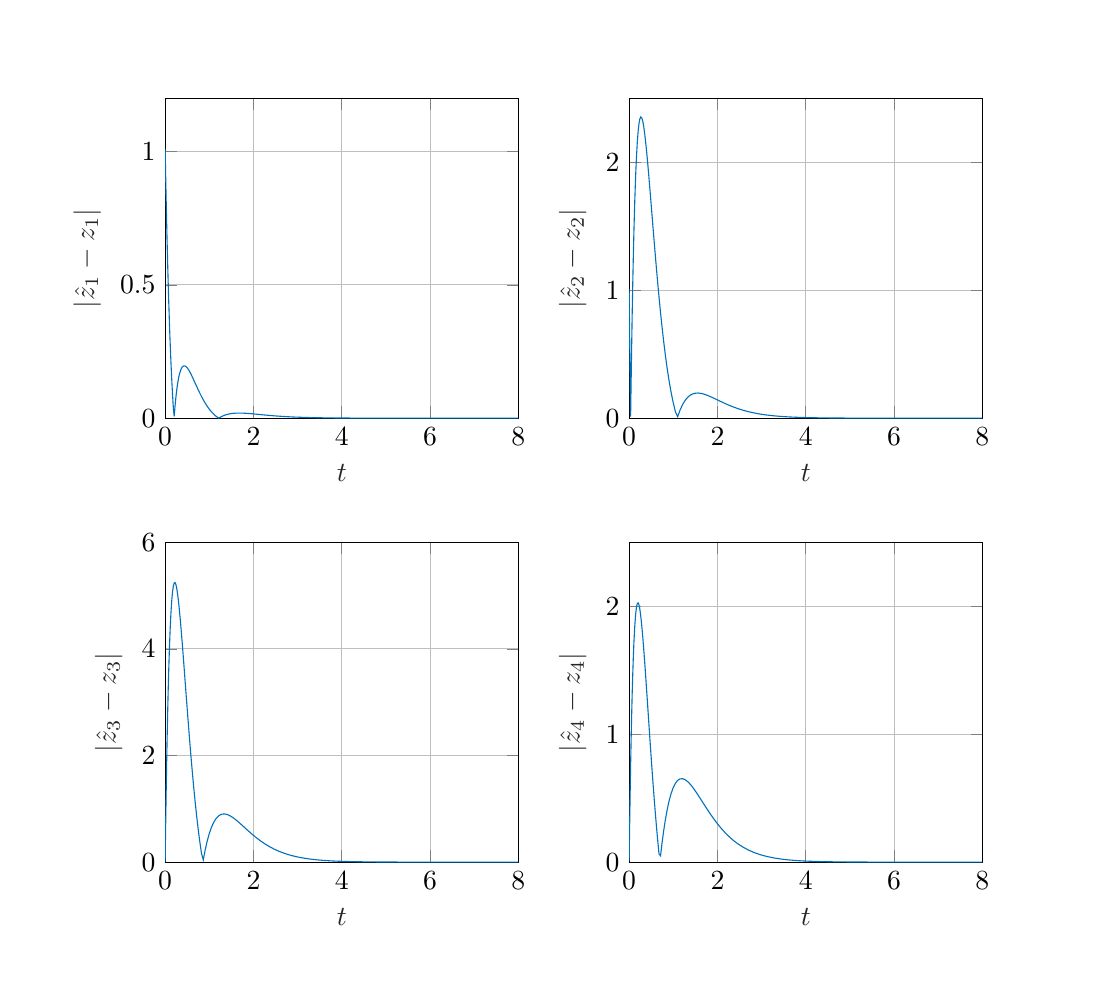
\begin{tikzpicture}

\begin{axis}[%
width=0.37\linewidth,
height=0.335\linewidth,
at={(0\linewidth,0.465\linewidth)},
scale only axis,
xmin=0,
xmax=8,
xlabel style={font=\color{white!15!black}},
xlabel={$t$},
ymin=0,
ymax=1.2,
ylabel style={font=\color{white!15!black}},
ylabel={$|\hat z_1 - z_1|$},
axis background/.style={fill=white},
xmajorgrids,
ymajorgrids
]
\addplot [color=mycolor1, forget plot]
  table[row sep=crcr]{%
0	1.01\\
8.79073862042456e-05	1.00921001156934\\
0.000175814772408491	1.00842044513877\\
0.000263722158612737	1.00763130051668\\
0.000351629544816982	1.00684257751155\\
0.00079116647583821	1.00290528004245\\
0.00123070340685944	0.998978494314363\\
0.00167024033788067	0.995062196476172\\
0.00210977726890189	0.991156362726237\\
0.00430746192400803	0.971783325584731\\
0.00650514657911417	0.952668348808015\\
0.00870283123422031	0.933808512457102\\
0.0109005158893265	0.915200926591713\\
0.0218889391648572	0.82584729806403\\
0.0328773624403879	0.742383563198636\\
0.0438657857159186	0.664481120551387\\
0.0548542089914493	0.591827260711443\\
0.0685213066794778	0.50833944966751\\
0.0821884043675063	0.431977480846399\\
0.0958555020555349	0.36223926631529\\
0.109522599743563	0.298652538781746\\
0.12847096298975	0.219848231185681\\
0.147419326235936	0.150943271964949\\
0.166367689482122	0.0909529736397753\\
0.185316052728308	0.038970485125204\\
0.204587811801823	0.00653665650794805\\
0.223859570875339	0.0453889775071512\\
0.243131329948854	0.0782945622995478\\
0.262403089022369	0.105903431153716\\
0.285682928723189	0.133029150497682\\
0.308962768424008	0.154194943298058\\
0.332242608124828	0.170212752832248\\
0.355522447825647	0.181816156265608\\
0.378209341421843	0.189495571207864\\
0.400896235018038	0.194109648331965\\
0.423583128614234	0.196116359978847\\
0.446270022210429	0.195928320762637\\
0.469960064767812	0.193782818170652\\
0.493650107325195	0.189989166875135\\
0.517340149882577	0.184855377788281\\
0.54103019243996	0.178656322298753\\
0.565990025188309	0.171234749729145\\
0.590949857936658	0.163123203244887\\
0.615909690685007	0.15451949857889\\
0.640869523433356	0.145597673008529\\
0.675923470192424	0.132813766215606\\
0.710977416951492	0.11999685545621\\
0.74603136371056	0.107382849801427\\
0.781085310469628	0.0951733911844026\\
0.822370774757663	0.0815169556860216\\
0.863656239045698	0.0687485391189142\\
0.904941703333733	0.0569429445386807\\
0.946227167621768	0.0461634197100915\\
0.997113834901503	0.0343302902372771\\
1.04800050218124	0.0240148050117223\\
1.09888716946097	0.0151178360173385\\
1.14977383674071	0.00756669439866253\\
1.21365213691803	0.000142023901560928\\
1.27753043709535	0.00617212879664231\\
1.34140873727267	0.0107889900589857\\
1.40528703744999	0.0141783284786869\\
1.48298426693461	0.0168989394072221\\
1.56068149641922	0.0184490249218625\\
1.63837872590384	0.0191227775596314\\
1.71607595538845	0.019121729149447\\
1.80164391168615	0.0185437797764578\\
1.88721186798386	0.0175764690223987\\
1.97277982428156	0.0163688405800815\\
2.05834778057926	0.0150326414428608\\
2.15857068511346	0.0134203983956391\\
2.25879358964765	0.0118326979079062\\
2.35901649418185	0.0103176251883514\\
2.45923939871604	0.00891985588385857\\
2.58569761462329	0.00737033819016908\\
2.71215583053053	0.00603353077248325\\
2.83861404643778	0.00488354538128455\\
2.96507226234503	0.00392425794906526\\
3.12372831083571	0.00298367870876248\\
3.2823843593264	0.00225298257096895\\
3.44104040781708	0.00167761714908554\\
3.59969645630776	0.00124001579544508\\
3.76741679336023	0.000905406703360256\\
3.9351371304127	0.000658856274220909\\
4.10285746746516	0.000479354623148964\\
4.27057780451763	0.000348126054129594\\
4.44478734191165	0.000246804086035723\\
4.61899687930568	0.000174714032453949\\
4.7932064166997	0.000125849774233799\\
4.96741595409372	9.10694838367476e-05\\
5.15878806324502	6.0844138534577e-05\\
5.35016017239631	4.06037158793282e-05\\
5.5415322815476	2.91084661423469e-05\\
5.7329043906989	2.13129634385467e-05\\
5.93083095054909	1.30843778336498e-05\\
6.12875751039928	7.99530369910428e-06\\
6.32668407024947	6.38203095171264e-06\\
6.52461063009966	5.32659360885646e-06\\
6.72461063009966	2.51692405583981e-06\\
6.92461063009966	1.0300447108591e-06\\
7.12461063009966	1.48583810677394e-06\\
7.32461063009966	1.80478098954495e-06\\
7.49345797257474	8.55382204179023e-07\\
7.66230531504983	3.52488855881461e-07\\
7.83115265752491	4.37536353814494e-07\\
8	5.23700569132757e-07\\
};
\end{axis}

\begin{axis}[%
width=0.37\linewidth,
height=0.335\linewidth,
at={(0.486\linewidth,0.465\linewidth)},
scale only axis,
xmin=0,
xmax=8,
xlabel style={font=\color{white!15!black}},
xlabel={$t$},
ymin=0,
ymax=2.5,
ylabel style={font=\color{white!15!black}},
ylabel={$|\hat z_2 - z_2|$},
axis background/.style={fill=white},
xmajorgrids,
ymajorgrids
]
\addplot [color=mycolor1, forget plot]
  table[row sep=crcr]{%
0	1.01\\
8.79073862042456e-05	1.00698071238301\\
0.000175814772408491	1.00396342249614\\
0.000263722158612737	1.00094812934907\\
0.000351629544816982	0.997934831951921\\
0.00079116647583821	0.982898246599377\\
0.00123070340685944	0.967911406761365\\
0.00167024033788067	0.95297418918767\\
0.00210977726890189	0.938086470895903\\
0.00430746192400803	0.864386082349487\\
0.00650514657911417	0.791904882215734\\
0.00870283123422031	0.720627796747768\\
0.0109005158893265	0.650539914418066\\
0.0218889391648572	0.317425725510196\\
0.0328773624403879	0.0118974607291932\\
0.0438657857159186	0.267732467235944\\
0.0548542089914493	0.523066151698034\\
0.0685213066794778	0.809022813809534\\
0.0821884043675063	1.06246016979725\\
0.0958555020555349	1.28592528419903\\
0.109522599743563	1.48180607813795\\
0.12847096298975	1.71188999768493\\
0.147419326235936	1.89861492934622\\
0.166367689482122	2.04688345556288\\
0.185316052728308	2.16118834560923\\
0.204587811801823	2.24679666931951\\
0.223859570875339	2.30525209745283\\
0.243131329948854	2.33998373658272\\
0.262403089022369	2.35411970732471\\
0.285682928723189	2.34773047552119\\
0.308962768424008	2.31967056284584\\
0.332242608124828	2.27371975184893\\
0.355522447825647	2.21326176942886\\
0.378209341421843	2.14320047276101\\
0.400896235018038	2.06443446843876\\
0.423583128614234	1.97897086269469\\
0.446270022210429	1.88859409523153\\
0.469960064767812	1.79064418712177\\
0.493650107325195	1.6904435407515\\
0.517340149882577	1.58922327678492\\
0.54103019243996	1.48805859403898\\
0.565990025188309	1.38252199843317\\
0.590949857936658	1.27885261140625\\
0.615909690685007	1.17771852392394\\
0.640869523433356	1.07968304005883\\
0.675923470192424	0.948087350481302\\
0.710977416951492	0.824218784136052\\
0.74603136371056	0.708529307288209\\
0.781085310469628	0.60135515740364\\
0.822370774757663	0.486227592008412\\
0.863656239045698	0.382739666742522\\
0.904941703333733	0.290411139003522\\
0.946227167621768	0.208787724648171\\
0.997113834901503	0.122091636516402\\
1.04800050218124	0.0492502947628686\\
1.09888716946097	0.0112341848745199\\
1.14977383674071	0.0606035668538987\\
1.21365213691803	0.108684322898833\\
1.27753043709535	0.143886164011749\\
1.34140873727267	0.168550160211364\\
1.40528703744999	0.184473884302012\\
1.48298426693461	0.194354049103757\\
1.56068149641922	0.196473856022677\\
1.63837872590384	0.192991054280076\\
1.71607595538845	0.185515577603189\\
1.80164391168615	0.174225597606465\\
1.88721186798386	0.161068374159603\\
1.97277982428156	0.146998524005849\\
2.05834778057926	0.132782570128614\\
2.15857068511346	0.116710903642669\\
2.25879358964765	0.101596579772261\\
2.35901649418185	0.0876418109059638\\
2.45923939871604	0.0750852630988086\\
2.58569761462329	0.0614517532037735\\
2.71215583053053	0.0499092326648305\\
2.83861404643778	0.0401405195721951\\
2.96507226234503	0.0320874026669276\\
3.12372831083571	0.0242474694485746\\
3.2823843593264	0.0182149915626564\\
3.44104040781708	0.0135200826659161\\
3.59969645630776	0.00997351214871189\\
3.76741679336023	0.00726294843192576\\
3.9351371304127	0.00527243700183\\
4.10285746746516	0.00382682003038659\\
4.27057780451763	0.00277394722369495\\
4.44478734191165	0.00196627480007749\\
4.61899687930568	0.00139146354375597\\
4.7932064166997	0.00099907300183455\\
4.96741595409372	0.000720372154604743\\
5.15878806324502	0.000483282384459827\\
5.35016017239631	0.000323687120329708\\
5.5415322815476	0.000229759968874865\\
5.7329043906989	0.000166170192021808\\
5.93083095054909	0.000104103298224661\\
6.12875751039928	6.49929281814621e-05\\
6.32668407024947	4.97720384988742e-05\\
6.52461063009966	3.97853482294597e-05\\
6.72461063009966	2.03390100950163e-05\\
6.92461063009966	9.65510209738341e-06\\
7.12461063009966	1.11649745246911e-05\\
7.32461063009966	1.22797905850458e-05\\
7.49345797257474	6.17942071201583e-06\\
7.66230531504983	2.86007476102412e-06\\
7.83115265752491	3.12101714938784e-06\\
8	3.46147942664743e-06\\
};
\end{axis}

\begin{axis}[%
width=0.37\linewidth,
height=0.335\linewidth,
at={(0\linewidth,0\linewidth)},
scale only axis,
xmin=0,
xmax=8,
xlabel style={font=\color{white!15!black}},
xlabel={$t$},
ymin=0,
ymax=6,
ylabel style={font=\color{white!15!black}},
ylabel={$|\hat z_3 - z_3|$},
axis background/.style={fill=white},
xmajorgrids,
ymajorgrids
]
\addplot [color=mycolor1, forget plot]
  table[row sep=crcr]{%
0	0.01\\
8.79073862042456e-05	0.0155153024171999\\
0.000175814772408491	0.0210264922780628\\
0.000263722158612737	0.0265335717278652\\
0.000351629544816982	0.0320365429109231\\
0.00079116647583821	0.0594898498093503\\
0.00123070340685944	0.0868407711344544\\
0.00167024033788067	0.114089573846806\\
0.00210977726890189	0.141236524310411\\
0.00430746192400803	0.275452775420603\\
0.00650514657911417	0.407162332514646\\
0.00870283123422031	0.536397825058002\\
0.0109005158893265	0.663191521381311\\
0.0218889391648572	1.26164233477263\\
0.0328773624403879	1.80368242375205\\
0.0438657857159186	2.2929529462601\\
0.0548542089914493	2.73290535908462\\
0.0685213066794778	3.21619633585047\\
0.0821884043675063	3.63407553496038\\
0.0958555020555349	3.99199600349462\\
0.109522599743563	4.29505947531853\\
0.12847096298975	4.63331303329858\\
0.147419326235936	4.88667151716522\\
0.166367689482122	5.06550595724409\\
0.185316052728308	5.17929056838182\\
0.204587811801823	5.23709214503925\\
0.223859570875339	5.24431130144167\\
0.243131329948854	5.2080721996805\\
0.262403089022369	5.13484697478791\\
0.285682928723189	5.00529985688154\\
0.308962768424008	4.8389465701348\\
0.332242608124828	4.64343323810618\\
0.355522447825647	4.42556234649271\\
0.378209341421843	4.19733286859482\\
0.400896235018038	3.95789220168822\\
0.423583128614234	3.71112876467556\\
0.446270022210429	3.46046595348098\\
0.469960064767812	3.19770626919033\\
0.493650107325195	2.93648668382745\\
0.517340149882577	2.67902313275378\\
0.54103019243996	2.42721559931071\\
0.565990025188309	2.16972518598367\\
0.590949857936658	1.92151376503093\\
0.615909690685007	1.6835971541416\\
0.640869523433356	1.45678921957908\\
0.675923470192424	1.1581357488129\\
0.710977416951492	0.883155697573164\\
0.74603136371056	0.631928320874614\\
0.781085310469628	0.404364325613442\\
0.822370774757663	0.166075575149968\\
0.863656239045698	0.0418676858715745\\
0.904941703333733	0.221459180090274\\
0.946227167621768	0.374526585413547\\
0.997113834901503	0.529563642741957\\
1.04800050218124	0.651796272448539\\
1.09888716946097	0.745437141191156\\
1.14977383674071	0.814001902876845\\
1.21365213691803	0.869607757099876\\
1.27753043709535	0.897784396933922\\
1.34140873727267	0.904338512347343\\
1.40528703744999	0.893769082588452\\
1.48298426693461	0.863432275855492\\
1.56068149641922	0.819919063549521\\
1.63837872590384	0.768044533434962\\
1.71607595538845	0.711423332757251\\
1.80164391168615	0.646963317154565\\
1.88721186798386	0.582852389481806\\
1.97277982428156	0.520822806739366\\
2.05834778057926	0.462275283016544\\
2.15857068511346	0.399404517203608\\
2.25879358964765	0.342770952078265\\
2.35901649418185	0.292246482472553\\
2.45923939871604	0.247917815007709\\
2.58569761462329	0.200677514269278\\
2.71215583053053	0.161500917493448\\
2.83861404643778	0.129007421963689\\
2.96507226234503	0.102565009118122\\
3.12372831083571	0.0769252477668321\\
3.2823843593264	0.0574231192211734\\
3.44104040781708	0.042498323267159\\
3.59969645630776	0.031310307981034\\
3.76741679336023	0.0227110308122658\\
3.9351371304127	0.0164289492015648\\
4.10285746746516	0.0119021039709626\\
4.27057780451763	0.00861993754950596\\
4.44478734191165	0.00610011330872062\\
4.61899687930568	0.00430979252894303\\
4.7932064166997	0.00308722907023196\\
4.96741595409372	0.0022213520926222\\
5.15878806324502	0.00149223384725161\\
5.35016017239631	0.00100038516143464\\
5.5415322815476	0.000705348684299167\\
5.7329043906989	0.000506118535174238\\
5.93083095054909	0.000320953719391781\\
6.12875751039928	0.00020281926046728\\
6.32668407024947	0.000150992913814818\\
6.52461063009966	0.000117018444822037\\
6.72461063009966	6.30324965023021e-05\\
6.92461063009966	3.24607642419039e-05\\
7.12461063009966	3.27526068328865e-05\\
7.32461063009966	3.32805497826882e-05\\
7.49345797257474	1.75265436048733e-05\\
7.66230531504983	8.73836404302608e-06\\
7.83115265752491	8.69628423316726e-06\\
8	9.04675749424655e-06\\
};
\end{axis}

\begin{axis}[%
width=0.37\linewidth,
height=0.335\linewidth,
at={(0.486\linewidth,0\linewidth)},
scale only axis,
xmin=0,
xmax=8,
xlabel style={font=\color{white!15!black}},
xlabel={$t$},
ymin=0,
ymax=2.5,
ylabel style={font=\color{white!15!black}},
ylabel={$|\hat z_4 - z_4|$},
axis background/.style={fill=white},
xmajorgrids,
ymajorgrids
]
\addplot [color=mycolor1, forget plot]
  table[row sep=crcr]{%
0	0.01\\
8.79073862042456e-05	0.0122885252483646\\
0.000175814772408491	0.0145752400797803\\
0.000263722158612737	0.0168601454665514\\
0.000351629544816982	0.0191432423805398\\
0.00079116647583821	0.0305316338431418\\
0.00123070340685944	0.0418749590110087\\
0.00167024033788067	0.0531733388696604\\
0.00210977726890189	0.0644268941297164\\
0.00430746192400803	0.120026507798134\\
0.00650514657911417	0.174523455318526\\
0.00870283123422031	0.227932518629783\\
0.0109005158893265	0.280268313314255\\
0.0218889391648572	0.526350563115968\\
0.0328773624403879	0.747698515636859\\
0.0438657857159186	0.94595842869224\\
0.0548542089914493	1.12268935143183\\
0.0685213066794778	1.31467575965707\\
0.0821884043675063	1.4782638990951\\
0.0958555020555349	1.61590753782461\\
0.109522599743563	1.7298994493919\\
0.12847096298975	1.85277529442146\\
0.147419326235936	1.93939745592554\\
0.166367689482122	1.99439838131744\\
0.185316052728308	2.02200175631496\\
0.204587811801823	2.02588589833426\\
0.223859570875339	2.00884385475086\\
0.243131329948854	1.97402213909438\\
0.262403089022369	1.9242719468088\\
0.285682928723189	1.84787978202068\\
0.308962768424008	1.75721537776627\\
0.332242608124828	1.6555988287501\\
0.355522447825647	1.54597218326012\\
0.378209341421843	1.43383878693866\\
0.400896235018038	1.31838291693991\\
0.423583128614234	1.20124518169758\\
0.446270022210429	1.08386043970211\\
0.469960064767812	0.962327026756757\\
0.493650107325195	0.842903161108843\\
0.517340149882577	0.72647544467005\\
0.54103019243996	0.613793461510474\\
0.565990025188309	0.499775766672975\\
0.590949857936658	0.391040899733875\\
0.615909690685007	0.287938757615396\\
0.640869523433356	0.19073469129159\\
0.675923470192424	0.0645025592485933\\
0.710977416951492	0.0497350227254345\\
0.74603136371056	0.152166015274701\\
0.781085310469628	0.243032317640924\\
0.822370774757663	0.335745357246501\\
0.863656239045698	0.414048652739508\\
0.904941703333733	0.479070529981964\\
0.946227167621768	0.531834889905088\\
0.997113834901503	0.581551951320635\\
1.04800050218124	0.616548594836744\\
1.09888716946097	0.638937760312653\\
1.14977383674071	0.650480690684709\\
1.21365213691803	0.652099112525486\\
1.27753043709535	0.642470390415999\\
1.34140873727267	0.624329779950344\\
1.40528703744999	0.599792210666256\\
1.48298426693461	0.563915957555627\\
1.56068149641922	0.524087367410093\\
1.63837872590384	0.482403853388066\\
1.71607595538845	0.440428611042509\\
1.80164391168615	0.395283776970299\\
1.88721186798386	0.352225371264359\\
1.97277982428156	0.3118458363665\\
2.05834778057926	0.274620175394129\\
2.15857068511346	0.235399969601864\\
2.25879358964765	0.200672723001404\\
2.35901649418185	0.170138298455917\\
2.45923939871604	0.143642044588862\\
2.58569761462329	0.115636722542087\\
2.71215583053053	0.0926335919329997\\
2.83861404643778	0.0737398046021589\\
2.96507226234503	0.05846117708598\\
3.12372831083571	0.0436721836714176\\
3.2823843593264	0.0324888618680319\\
3.44104040781708	0.0240055019948873\\
3.59969645630776	0.0176717478338175\\
3.76741679336023	0.0127877666894216\\
3.9351371304127	0.00923021640976618\\
4.10285746746516	0.00667840969029454\\
4.27057780451763	0.00483298281321631\\
4.44478734191165	0.00341499730718997\\
4.61899687930568	0.00240885189449513\\
4.7932064166997	0.00172235196748316\\
4.96741595409372	0.00123709098582636\\
5.15878806324502	0.000830335731748844\\
5.35016017239631	0.000555899786406799\\
5.5415322815476	0.000390111112394731\\
5.7329043906989	0.000278439029208655\\
5.93083095054909	0.000176978920872706\\
6.12875751039928	0.000111960958726898\\
6.32668407024947	8.20372102141587e-05\\
6.52461063009966	6.24982719832357e-05\\
6.72461063009966	3.41412957028941e-05\\
6.92461063009966	1.7881162700073e-05\\
7.12461063009966	1.70569565556278e-05\\
7.32461063009966	1.67227856322505e-05\\
7.49345797257474	8.82789162282016e-06\\
7.66230531504983	4.38486875609101e-06\\
7.83115265752491	4.20898667097269e-06\\
8	4.28096345417295e-06\\
};
\end{axis}

\begin{axis}[%
width=1.104\linewidth,
height=0.982\linewidth,
at={(-0.144\linewidth,-0.108\linewidth)},
scale only axis,
xmin=0,
xmax=1,
ymin=0,
ymax=1,
axis line style={draw=none},
ticks=none,
axis x line*=bottom,
axis y line*=left
]
\end{axis}
\end{tikzpicture}%
	\caption{Абсолютное отклонение оценки от настоящего состояния линейной системы для предыдущей задачи.}
\end{figure}

\begin{figure}[t]
	\centering
	% This file was created by matlab2tikz.
%
%The latest updates can be retrieved from
%  http://www.mathworks.com/matlabcentral/fileexchange/22022-matlab2tikz-matlab2tikz
%where you can also make suggestions and rate matlab2tikz.
%
\definecolor{mycolor1}{rgb}{0.00000,0.44700,0.74100}%
%
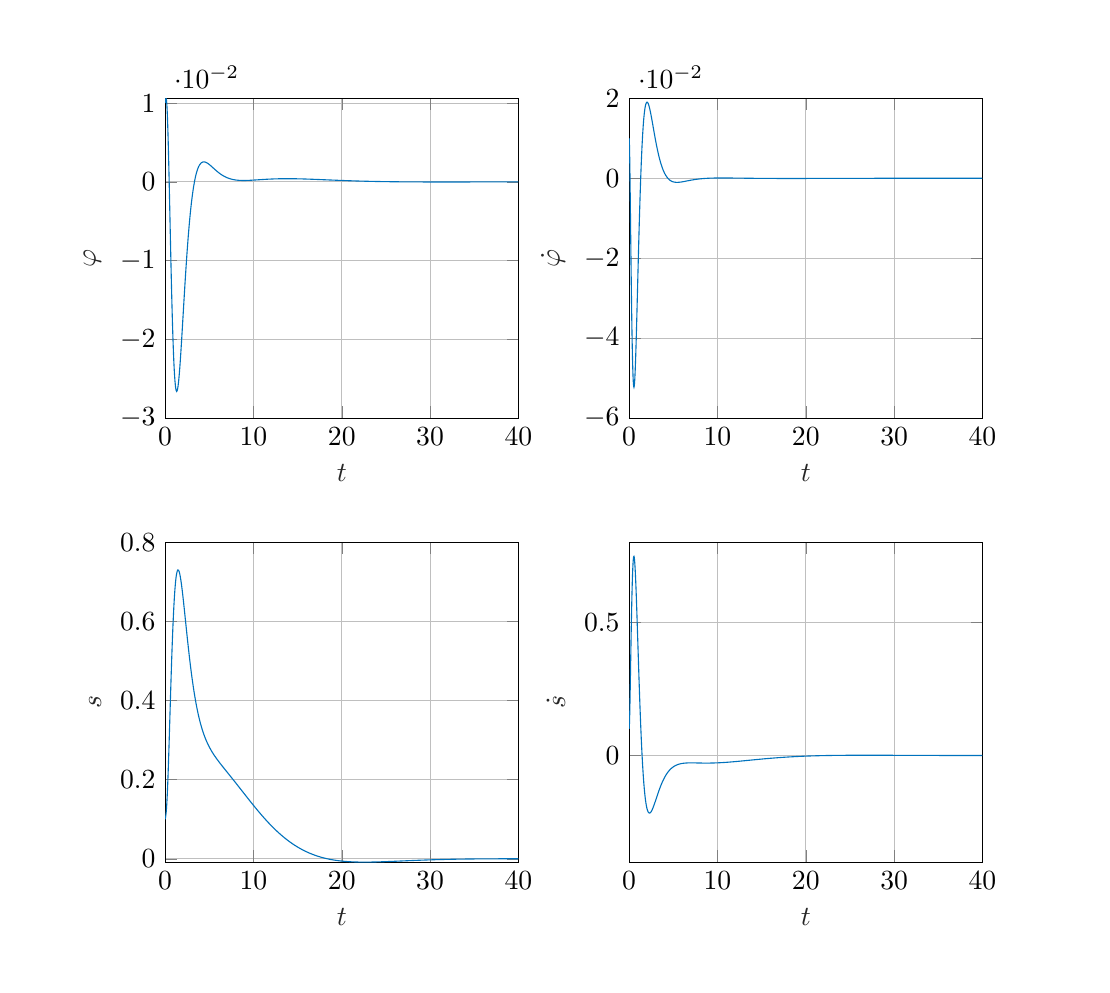
\begin{tikzpicture}

\begin{axis}[%
width=0.37\linewidth,
height=0.335\linewidth,
at={(0\linewidth,0.465\linewidth)},
scale only axis,
xmin=0,
xmax=40,
xlabel style={font=\color{white!15!black}},
xlabel={$t$},
ymin=-0.03,
ymax=0.0106075978485443,
ylabel style={font=\color{white!15!black}},
ylabel={$\varphi$},
axis background/.style={fill=white},
xmajorgrids,
ymajorgrids
]
\addplot [color=mycolor1, forget plot]
  table[row sep=crcr]{%
0	0.01\\
0.000821791019927233	0.0100082149689288\\
0.00164358203985447	0.0100164230501642\\
0.0024653730597817	0.0100246227453925\\
0.00328716407970893	0.0100328125688547\\
0.0073961191793451	0.0100735623985014\\
0.0115050742789813	0.010113849755686\\
0.0156140293786174	0.0101535027700436\\
0.0197229844782536	0.0101923567649445\\
0.0387608823959644	0.0103573807363085\\
0.0577987803136751	0.0104884456599405\\
0.0768366782313859	0.0105747855754633\\
0.0958745761490967	0.0106075978485443\\
0.113362875779606	0.010584880458077\\
0.130851175410116	0.0105082043356513\\
0.148339475040626	0.0103753172284924\\
0.165827774671136	0.0101847652402853\\
0.188844483406901	0.00984510516343644\\
0.211861192142666	0.00940595815404465\\
0.234877900878431	0.00887035271865\\
0.257894609614196	0.00824213486390125\\
0.286451652811934	0.00734140359351964\\
0.315008696009671	0.00631882694082847\\
0.343565739207409	0.00518837860195674\\
0.372122782405147	0.00396360585978825\\
0.406266880391565	0.00239479878603874\\
0.440410978377984	0.000737539717969546\\
0.474555076364403	-0.00098308765757968\\
0.508699174350821	-0.00274483342659041\\
0.54279359208006	-0.00452421005909274\\
0.576888009809299	-0.00630285523321597\\
0.610982427538538	-0.00806249124894127\\
0.645076845267777	-0.00978738659945619\\
0.689147209186533	-0.0119432554762108\\
0.733217573105289	-0.013991766714381\\
0.777287937024045	-0.015911924195125\\
0.821358300942801	-0.0176881779949299\\
0.876057604248058	-0.0196756203359694\\
0.930756907553314	-0.0214097215525735\\
0.98545621085857	-0.0228844180816182\\
1.04015551416383	-0.0240995975966661\\
1.10614002003457	-0.0252268037264578\\
1.17212452590531	-0.0260027048438441\\
1.23810903177604	-0.0264526302041283\\
1.30409353764678	-0.0266026856675677\\
1.37723575038186	-0.0264528519463644\\
1.45037796311694	-0.0260160461371086\\
1.52352017585202	-0.025337077763308\\
1.5966623885871	-0.024455132860584\\
1.6603502939681	-0.0235508506540024\\
1.72403819934911	-0.0225466634210346\\
1.78772610473011	-0.0214650215242292\\
1.85141401011111	-0.0203256538106125\\
1.92429316922088	-0.0189737737260156\\
1.99717232833065	-0.0175938872249242\\
2.07005148744042	-0.0162067450172813\\
2.14293064655019	-0.0148295758924733\\
2.23306543988133	-0.0131615607998245\\
2.32320023321248	-0.0115528544239707\\
2.41333502654363	-0.0100199806647674\\
2.50346981987478	-0.00857506225211287\\
2.61684746292718	-0.00689544644594481\\
2.73022510597958	-0.00537565525545281\\
2.84360274903198	-0.00401692714471724\\
2.95698039208438	-0.00281803606715\\
3.07885390623398	-0.00170228308322382\\
3.20072742038359	-0.000752836985841048\\
3.3226009345332	4.42419382329375e-05\\
3.44447444868281	0.000701411163264814\\
3.55341378857437	0.00118105197373295\\
3.66235312846594	0.00157067236163586\\
3.7712924683575	0.00188036256249684\\
3.88023180824907	0.00211916999165253\\
4.00507089330387	0.00231661976348046\\
4.12990997835866	0.00244486497992582\\
4.25474906341346	0.00251517645013366\\
4.37958814846826	0.00253724246277169\\
4.50120601686873	0.00252057702377805\\
4.62282388526921	0.00247369631434993\\
4.74444175366968	0.00240289656508469\\
4.86605962207016	0.00231360963660971\\
5.0056119686397	0.00219443097387457\\
5.14516431520924	0.0020630209501453\\
5.28471666177879	0.00192427155792788\\
5.42426900834833	0.00178226845846734\\
5.6253431494813	0.00157869541193337\\
5.82641729061426	0.00138201944070937\\
6.02749143174723	0.00119679794735139\\
6.2285655728802	0.00102668869062031\\
6.42333799985132	0.000878457904525748\\
6.61811042682243	0.000746621232576443\\
6.81288285379355	0.00063096493043055\\
7.00765528076467	0.000531260901127875\\
7.20534790137257	0.000445768363592296\\
7.40304052198046	0.000374688385910346\\
7.60073314258836	0.000316691906892318\\
7.79842576319625	0.000270618392168729\\
8.02364416846946	0.000231154483633863\\
8.24886257374266	0.000203549866468317\\
8.47408097901587	0.000185951852515081\\
8.69929938428907	0.000176822291521973\\
8.9636685853292	0.000175016152239526\\
9.22803778636933	0.000180622170384664\\
9.49240698740947	0.000191719112064909\\
9.7567761884496	0.000206798645705231\\
10.0733111578165	0.00022838721240517\\
10.3898461271834	0.000251797443035266\\
10.7063810965504	0.000275451506895233\\
11.0229160659173	0.000298535209243221\\
11.200671347673	0.000311047379109701\\
11.3784266294287	0.000322907717514071\\
11.5561819111844	0.000333993025860962\\
11.7339371929401	0.000344337483489923\\
11.9116924746958	0.000353956680514147\\
12.0894477564515	0.000362702785822623\\
12.2672030382072	0.000370534494704773\\
12.4449583199629	0.000377479321563349\\
12.6765770512804	0.000385250920589362\\
12.9081957825979	0.000391467995516795\\
13.1398145139154	0.000396116122719266\\
13.3714332452329	0.000399333866645948\\
13.6348054673248	0.000401540855441926\\
13.8981776894167	0.000401878827546821\\
14.1615499115086	0.000400257564761774\\
14.4249221336005	0.000397265956984214\\
14.5941445771904	0.000394869409960984\\
14.7633670207803	0.000391845065477303\\
14.9325894643701	0.000388187447752793\\
15.10181190796	0.000384061993977549\\
15.2710343515499	0.000379587135038451\\
15.4402567951398	0.000374669679935002\\
15.6094792387297	0.000369328001156317\\
15.7787016823196	0.000363636715727823\\
15.9992483184829	0.000355801154127665\\
16.2197949546462	0.000347451181231986\\
16.4403415908095	0.000338616916688053\\
16.6608882269728	0.000329433207519509\\
16.9204693872244	0.000318411357208951\\
17.1800505474759	0.000306938683152203\\
17.4396317077274	0.000294958644786313\\
17.6992128679789	0.000282877796031078\\
17.859623309804	0.000275516251245844\\
18.0200337516291	0.000268072159115142\\
18.1804441934542	0.000260544354984091\\
18.3408546352793	0.000253014342254086\\
18.5012650771044	0.000245538239092314\\
18.6616755189294	0.000238070636214807\\
18.8220859607545	0.00023061884521698\\
18.9824964025796	0.000223211642132316\\
19.1927910900236	0.00021360709768489\\
19.4030857774676	0.000204106803048489\\
19.6133804649116	0.000194719990945935\\
19.8236751523556	0.000185488924896534\\
20.0732106097773	0.000174802864777728\\
20.3227460671991	0.000164345983853064\\
20.5722815246209	0.000154103340858166\\
20.8218169820427	0.000144176090493989\\
20.9780322858865	0.000138159648358262\\
21.1342475897304	0.000132254672830258\\
21.2904628935742	0.00012646074205019\\
21.4466781974181	0.000120794977042244\\
21.6028935012619	0.000115268704369419\\
21.7591088051058	0.000109871398027928\\
21.9153241089496	0.000104603585934486\\
22.0715394127935	9.94698341121316e-05\\
22.276732423891	9.2935584897624e-05\\
22.4819254349886	8.66328506849899e-05\\
22.6871184460862	8.05600227125326e-05\\
22.8923114571837	7.47211212570675e-05\\
23.1540290287523	6.76216087111843e-05\\
23.4157466003209	6.08889956096176e-05\\
23.6774641718895	5.45095670108991e-05\\
23.9391817434581	4.84981023509479e-05\\
24.1278444203235	4.44000153110678e-05\\
24.3165070971888	4.04776701619955e-05\\
24.5051697740542	3.67238263991448e-05\\
24.6938324509195	3.31462928766922e-05\\
24.8824951277849	2.97495355694121e-05\\
25.0711578046502	2.65167083501915e-05\\
25.2598204815156	2.34415460674791e-05\\
25.448483158381	2.05265930737662e-05\\
25.6695147066086	1.73173820569995e-05\\
25.8905462548362	1.43102717197828e-05\\
26.1115778030638	1.14940833770741e-05\\
26.3326093512914	8.87228661368437e-06\\
26.5721649013934	6.25700673333019e-06\\
26.8117204514954	3.84081311517281e-06\\
27.0512760015974	1.60363826341635e-06\\
27.2908315516994	-4.36802408013946e-07\\
27.5081082441846	-2.10060503353812e-06\\
27.7253849366698	-3.63584211713927e-06\\
27.942661629155	-5.06333203299923e-06\\
28.1599383216402	-6.35384871983108e-06\\
28.3438666039473	-7.32294256997281e-06\\
28.5277948862544	-8.21673088649177e-06\\
28.7117231685616	-9.04470508767313e-06\\
28.8956514508687	-9.79347487648768e-06\\
29.0734598356916	-1.04343769741109e-05\\
29.2512682205144	-1.10138619314022e-05\\
29.4290766053373	-1.15372614859309e-05\\
29.6068849901602	-1.20005540720853e-05\\
29.8115546668976	-1.24565008837615e-05\\
30.016224343635	-1.28451193994206e-05\\
30.2208940203725	-1.31734082419684e-05\\
30.4255636971099	-1.34383278160812e-05\\
30.6630173899931	-1.366122404357e-05\\
30.9004710828763	-1.38179948011946e-05\\
31.1379247757594	-1.39215594744924e-05\\
31.3753784686426	-1.39598690834144e-05\\
31.6094150241588	-1.39172356313636e-05\\
31.8434515796749	-1.38385222459925e-05\\
32.077488135191	-1.37437782536932e-05\\
32.3115246907072	-1.35994534118822e-05\\
32.5089311981757	-1.34169298362681e-05\\
32.7063377056441	-1.32234838416035e-05\\
32.9037442131126	-1.30316342526802e-05\\
33.1011507205811	-1.2815870167016e-05\\
33.2753568944668	-1.25913355045824e-05\\
33.4495630683526	-1.23606206129568e-05\\
33.6237692422383	-1.2127934129378e-05\\
33.7979754161241	-1.18847281486796e-05\\
33.9856971577928	-1.16045892131884e-05\\
34.1734188994616	-1.1318894619861e-05\\
34.3611406411303	-1.10309774612547e-05\\
34.5488623827991	-1.07361687412202e-05\\
34.7736964234946	-1.03683119670382e-05\\
34.9985304641901	-9.99906797766813e-06\\
35.2233645048856	-9.634367745163e-06\\
35.4481985455811	-9.26531351687162e-06\\
35.6923142740081	-8.84527507948295e-06\\
35.9364300024351	-8.43637105394015e-06\\
36.180545730862	-8.0525170275101e-06\\
36.424661459289	-7.66501319466856e-06\\
36.6413566677701	-7.29231869668666e-06\\
36.8580518762513	-6.93982186828959e-06\\
37.0747470847324	-6.62393221830379e-06\\
37.2914422932135	-6.30595008320043e-06\\
37.4712747928091	-6.0188421317657e-06\\
37.6511072924047	-5.74589800720592e-06\\
37.8309397920003	-5.49269632656899e-06\\
38.0107722915959	-5.24308036371745e-06\\
38.1857386189263	-4.99332539054222e-06\\
38.3607049462566	-4.75280576707991e-06\\
38.535671273587	-4.52357223572036e-06\\
38.7106376009173	-4.29949441214386e-06\\
38.9167555891731	-4.0360261299749e-06\\
39.1228735774289	-3.78361159252873e-06\\
39.3289915656846	-3.54495053243183e-06\\
39.5351095539404	-3.31337519984082e-06\\
39.6513321654553	-3.18378393048401e-06\\
39.7675547769702	-3.05736950793534e-06\\
39.8837773884851	-2.93405950731739e-06\\
40	-2.81357873436746e-06\\
};
\end{axis}

\begin{axis}[%
width=0.37\linewidth,
height=0.335\linewidth,
at={(0.486\linewidth,0.465\linewidth)},
scale only axis,
xmin=0,
xmax=40,
xlabel style={font=\color{white!15!black}},
xlabel={$t$},
ymin=-0.06,
ymax=0.02,
ylabel style={font=\color{white!15!black}},
ylabel={$\dot \varphi$},
axis background/.style={fill=white},
xmajorgrids,
ymajorgrids
]
\addplot [color=mycolor1, forget plot]
  table[row sep=crcr]{%
0	0.01\\
0.000821791019927233	0.00999253542326168\\
0.00164358203985447	0.00998323989496821\\
0.0024653730597817	0.0099721288020313\\
0.00328716407970893	0.00995921744826879\\
0.0073961191793451	0.00986818706302122\\
0.0115050742789813	0.00973439813246491\\
0.0156140293786174	0.00955967165399406\\
0.0197229844782536	0.00934578024467858\\
0.0387608823959644	0.00789328386343757\\
0.0577987803136751	0.00579345888602755\\
0.0768366782313859	0.00318441870203541\\
0.0958745761490967	0.000189362919317447\\
0.113362875779606	-0.00280998463730455\\
0.130851175410116	-0.00597480518639891\\
0.148339475040626	-0.00924335740886614\\
0.165827774671136	-0.0125609393916206\\
0.188844483406901	-0.0169225689892183\\
0.211861192142666	-0.0212012862497501\\
0.234877900878431	-0.0253270822131241\\
0.257894609614196	-0.0292412653307186\\
0.286451652811934	-0.0337348671167008\\
0.315008696009671	-0.0377785675627327\\
0.343565739207409	-0.0413372250418078\\
0.372122782405147	-0.0443857502119593\\
0.406266880391565	-0.0473458954083837\\
0.440410978377984	-0.0495808455548856\\
0.474555076364403	-0.0511222642390016\\
0.508699174350821	-0.0520030364148683\\
0.54279359208006	-0.0522654824040337\\
0.576888009809299	-0.0519720300764026\\
0.610982427538538	-0.0511811224776746\\
0.645076845267777	-0.0499471128714066\\
0.689147209186533	-0.0477823290368167\\
0.733217573105289	-0.0450931251928504\\
0.777287937024045	-0.0419951855454038\\
0.821358300942801	-0.0385855720062687\\
0.876057604248058	-0.0340512435993897\\
0.930756907553314	-0.029336293698704\\
0.98545621085857	-0.0245752550175624\\
1.04015551416383	-0.019869930865666\\
1.10614002003457	-0.0143849223208055\\
1.17212452590531	-0.00921991228212745\\
1.23810903177604	-0.00445385442607715\\
1.30409353764678	-0.000136647528927697\\
1.37723575038186	0.00408959231716509\\
1.45037796311694	0.00772381409001971\\
1.52352017585202	0.0107822145810688\\
1.5966623885871	0.0132861310991944\\
1.6603502939681	0.0150396140722737\\
1.72403819934911	0.0164303067690922\\
1.78772610473011	0.0174905187590986\\
1.85141401011111	0.0182504780398623\\
1.92429316922088	0.0187904925620335\\
1.99717232833065	0.0190263090233563\\
2.07005148744042	0.0190034477844562\\
2.14293064655019	0.0187614696771497\\
2.23306543988133	0.0182130303769822\\
2.32320023321248	0.0174520970048699\\
2.41333502654363	0.0165358406355136\\
2.50346981987478	0.0155101051462689\\
2.61684746292718	0.0141240966338944\\
2.73022510597958	0.0126926296721929\\
2.84360274903198	0.0112653027040431\\
2.95698039208438	0.00987846757696831\\
3.07885390623398	0.00846352900082273\\
3.20072742038359	0.00714682773086323\\
3.3226009345332	0.00593947108209778\\
3.44447444868281	0.00484925958945905\\
3.55341378857437	0.00397612457673932\\
3.66235312846594	0.00319500550048617\\
3.7712924683575	0.00250169435358138\\
3.88023180824907	0.0018920726302706\\
4.00507089330387	0.00129012002643591\\
4.12990997835866	0.000781443695521613\\
4.25474906341346	0.000356274938349044\\
4.37958814846826	6.22467946945291e-06\\
4.50120601686873	-0.000270342678982267\\
4.62282388526921	-0.000491723848928911\\
4.74444175366968	-0.000665184171827618\\
4.86605962207016	-0.000797053851034617\\
5.0056119686397	-0.000904567111257956\\
5.14516431520924	-0.000973165951255584\\
5.28471666177879	-0.0010099435823741\\
5.42426900834833	-0.00102090471652983\\
5.6253431494813	-0.00100175589217125\\
5.82641729061426	-0.000952758926348371\\
6.02749143174723	-0.000884020569096941\\
6.2285655728802	-0.000803478734439923\\
6.42333799985132	-0.000720021136621993\\
6.61811042682243	-0.000635091276096592\\
6.81288285379355	-0.000551434646595851\\
7.00765528076467	-0.00047135785482271\\
7.20534790137257	-0.000395407523065885\\
7.40304052198046	-0.000325402613967456\\
7.60073314258836	-0.000261707150418038\\
7.79842576319625	-0.000204644693042856\\
8.02364416846946	-0.000147830678367146\\
8.24886257374266	-9.91206835620904e-05\\
8.47408097901587	-5.78852546235589e-05\\
8.69929938428907	-2.36633270762207e-05\\
8.9636685853292	8.25286309346758e-06\\
9.22803778636933	3.26188983345314e-05\\
9.49240698740947	5.06229935826435e-05\\
9.7567761884496	6.30605908042694e-05\\
10.0733111578165	7.13128665291634e-05\\
10.3898461271834	7.47042943610771e-05\\
10.7063810965504	7.49547424111242e-05\\
11.0229160659173	7.17710033105031e-05\\
11.200671347673	6.82967224190836e-05\\
11.3784266294287	6.45074335063331e-05\\
11.5561819111844	6.0650854695663e-05\\
11.7339371929401	5.63964669172845e-05\\
11.9116924746958	5.1542793855457e-05\\
12.0894477564515	4.66044582316387e-05\\
12.2672030382072	4.17057309646331e-05\\
12.4449583199629	3.67233087435031e-05\\
12.6765770512804	2.99213677985777e-05\\
12.9081957825979	2.3331965853785e-05\\
13.1398145139154	1.71965108674126e-05\\
13.3714332452329	1.11691634035239e-05\\
13.6348054673248	3.61423351091444e-06\\
13.8981776894167	-2.95729425964009e-06\\
14.1615499115086	-7.71941715536682e-06\\
14.4249221336005	-1.25704472209453e-05\\
14.5941445771904	-1.65117709403457e-05\\
14.7633670207803	-1.99133726937703e-05\\
14.9325894643701	-2.26251024590683e-05\\
15.10181190796	-2.51828169925827e-05\\
15.2710343515499	-2.79360851317388e-05\\
15.4402567951398	-3.03888418489593e-05\\
15.6094792387297	-3.24944517831499e-05\\
15.7787016823196	-3.44348843681445e-05\\
15.9992483184829	-3.69557765954101e-05\\
16.2197949546462	-3.90781645880874e-05\\
16.4403415908095	-4.06898833899416e-05\\
16.6608882269728	-4.21103708060922e-05\\
16.9204693872244	-4.41948940990481e-05\\
17.1800505474759	-4.55366598544831e-05\\
17.4396317077274	-4.56101235421395e-05\\
17.6992128679789	-4.57658881886622e-05\\
17.859623309804	-4.64090153406575e-05\\
18.0200337516291	-4.67536850387443e-05\\
18.1804441934542	-4.67422809011836e-05\\
18.3408546352793	-4.6650842238261e-05\\
18.5012650771044	-4.66567954466109e-05\\
18.6616755189294	-4.65343623311341e-05\\
18.8220859607545	-4.62714109596135e-05\\
18.9824964025796	-4.59443345679388e-05\\
19.1927910900236	-4.551275672074e-05\\
19.4030857774676	-4.49451993935203e-05\\
19.6133804649116	-4.42112495221444e-05\\
19.8236751523556	-4.3419296963296e-05\\
20.0732106097773	-4.25919264042084e-05\\
20.3227460671991	-4.15681987706957e-05\\
20.5722815246209	-4.02214096854735e-05\\
20.8218169820427	-3.88995292457639e-05\\
20.9780322858865	-3.82145852884144e-05\\
21.1342475897304	-3.74632476328233e-05\\
21.2904628935742	-3.66358402742519e-05\\
21.4466781974181	-3.57941203918166e-05\\
21.6028935012619	-3.49779248227443e-05\\
21.7591088051058	-3.41409657201985e-05\\
21.9153241089496	-3.32822653426032e-05\\
22.0715394127935	-3.24180155717297e-05\\
22.276732423891	-3.12941770704355e-05\\
22.4819254349886	-3.01601840190183e-05\\
22.6871184460862	-2.90124797439743e-05\\
22.8923114571837	-2.78722497149279e-05\\
23.1540290287523	-2.64739774924313e-05\\
23.4157466003209	-2.50659991521015e-05\\
23.6774641718895	-2.36187549685401e-05\\
23.9391817434581	-2.22202604996168e-05\\
24.1278444203235	-2.12891547693721e-05\\
24.3165070971888	-2.03520427035798e-05\\
24.5051697740542	-1.9394175926698e-05\\
24.6938324509195	-1.84615906497325e-05\\
24.8824951277849	-1.7587552063785e-05\\
25.0711578046502	-1.672073442579e-05\\
25.2598204815156	-1.58525256785607e-05\\
25.448483158381	-1.50098466891062e-05\\
25.6695147066086	-1.40862418045832e-05\\
25.8905462548362	-1.31779179023944e-05\\
26.1115778030638	-1.22684581066889e-05\\
26.3326093512914	-1.14001028278633e-05\\
26.5721649013934	-1.05653416247372e-05\\
26.8117204514954	-9.73177783170164e-06\\
27.0512760015974	-8.85540466477585e-06\\
27.2908315516994	-8.04290576879339e-06\\
27.5081082441846	-7.45786924911837e-06\\
27.7253849366698	-6.84771350488537e-06\\
27.942661629155	-6.15498196307488e-06\\
28.1599383216402	-5.5218851561976e-06\\
28.3438666039473	-5.11618541694742e-06\\
28.5277948862544	-4.69445435070548e-06\\
28.7117231685616	-4.23324189787848e-06\\
28.8956514508687	-3.80030581861389e-06\\
29.0734598356916	-3.45234716687411e-06\\
29.2512682205144	-3.10566224606461e-06\\
29.4290766053373	-2.75091115854475e-06\\
29.6068849901602	-2.41586050472073e-06\\
29.8115546668976	-2.08105107932563e-06\\
30.016224343635	-1.75504318401785e-06\\
30.2208940203725	-1.42617045997147e-06\\
30.4255636971099	-1.12235574198622e-06\\
30.6630173899931	-8.41528843717046e-07\\
30.9004710828763	-5.61057454065035e-07\\
31.1379247757594	-2.51112923256864e-07\\
31.3753784686426	1.92725633785755e-08\\
31.6094150241588	1.61569565681367e-07\\
31.8434515796749	3.37303032774085e-07\\
32.077488135191	6.09489777456015e-07\\
32.3115246907072	8.27642385088679e-07\\
32.5089311981757	8.6930247440333e-07\\
32.7063377056441	9.501816963917e-07\\
32.9037442131126	1.11200848569411e-06\\
33.1011507205811	1.24480394879063e-06\\
33.2753568944668	1.2748031165031e-06\\
33.4495630683526	1.32118803930252e-06\\
33.6237692422383	1.39611419776337e-06\\
33.7979754161241	1.46093654952115e-06\\
33.9856971577928	1.48947018001745e-06\\
34.1734188994616	1.52299971298868e-06\\
34.3611406411303	1.57013786015638e-06\\
34.5488623827991	1.6077591881069e-06\\
34.7736964234946	1.61166260967437e-06\\
34.9985304641901	1.62324588737684e-06\\
35.2233645048856	1.66006006501779e-06\\
35.4481985455811	1.68081454099194e-06\\
35.6923142740081	1.62146455874488e-06\\
35.9364300024351	1.59603002707187e-06\\
36.180545730862	1.65468747602748e-06\\
36.424661459289	1.67768455037917e-06\\
36.6413566677701	1.56200697446432e-06\\
36.8580518762513	1.50429874132296e-06\\
37.0747470847324	1.5677440641166e-06\\
37.2914422932135	1.59535395829487e-06\\
37.4712747928091	1.50315074378624e-06\\
37.6511072924047	1.44639684122583e-06\\
37.8309397920003	1.44655345626799e-06\\
38.0107722915959	1.43824122845413e-06\\
38.1857386189263	1.38006541828276e-06\\
38.3607049462566	1.33611347882492e-06\\
38.535671273587	1.31415977789715e-06\\
38.7106376009173	1.28932644494687e-06\\
38.9167555891731	1.23155753673311e-06\\
39.1228735774289	1.18466245028458e-06\\
39.3289915656846	1.15922532379993e-06\\
39.5351095539404	1.12846493750954e-06\\
39.6513321654553	1.10021467508353e-06\\
39.7675547769702	1.07398039721957e-06\\
39.8837773884851	1.04949575365412e-06\\
40	1.02569182820205e-06\\
};
\end{axis}

\begin{axis}[%
width=0.37\linewidth,
height=0.335\linewidth,
at={(0\linewidth,0\linewidth)},
scale only axis,
xmin=0,
xmax=40,
xlabel style={font=\color{white!15!black}},
xlabel={$t$},
ymin=-0.00814482048916752,
ymax=0.8,
ylabel style={font=\color{white!15!black}},
ylabel={$s$},
axis background/.style={fill=white},
xmajorgrids,
ymajorgrids
]
\addplot [color=mycolor1, forget plot]
  table[row sep=crcr]{%
0	0.1\\
0.000821791019927233	0.100082233849074\\
0.00164358203985447	0.100164587272087\\
0.0024653730597817	0.100247075294511\\
0.00328716407970893	0.100329712816222\\
0.0073961191793451	0.100745656491857\\
0.0115050742789813	0.101167500741662\\
0.0156140293786174	0.101596969466897\\
0.0197229844782536	0.102035714526415\\
0.0387608823959644	0.10423540804782\\
0.0577987803136751	0.106802871477116\\
0.0768366782313859	0.109846153706908\\
0.0958745761490967	0.11345347560003\\
0.113362875779606	0.117321162453518\\
0.130851175410116	0.121752740524897\\
0.148339475040626	0.126770565711725\\
0.165827774671136	0.132388859419647\\
0.188844483406901	0.14070744268891\\
0.211861192142666	0.15006003467621\\
0.234877900878431	0.160414620949113\\
0.257894609614196	0.171730583953384\\
0.286451652811934	0.187028551872646\\
0.315008696009671	0.203589844808994\\
0.343565739207409	0.22126848041191\\
0.372122782405147	0.239922064166317\\
0.406266880391565	0.26330041866171\\
0.440410978377984	0.28758413790514\\
0.474555076364403	0.312507863554362\\
0.508699174350821	0.337834156593266\\
0.54279359208006	0.36330169994694\\
0.576888009809299	0.388722446306755\\
0.610982427538538	0.413898047437043\\
0.645076845267777	0.438655969544741\\
0.689147209186533	0.469792519117885\\
0.733217573105289	0.499681454245604\\
0.777287937024045	0.528082686164776\\
0.821358300942801	0.554813077971318\\
0.876057604248058	0.58545778275603\\
0.930756907553314	0.613127293267465\\
0.98545621085857	0.637721412352899\\
1.04015551416383	0.65920654217182\\
1.10614002003457	0.68101621255186\\
1.17212452590531	0.698488611057944\\
1.23810903177604	0.711851066893657\\
1.30409353764678	0.721350565835323\\
1.37723575038186	0.727703578812851\\
1.45037796311694	0.730125427966427\\
1.52352017585202	0.729081978200196\\
1.5966623885871	0.72499193810245\\
1.6603502939681	0.719266175845632\\
1.72403819934911	0.711824946890276\\
1.78772610473011	0.702923625939974\\
1.85141401011111	0.692791956183403\\
1.92429316922088	0.679959892133486\\
1.99717232833065	0.666092161783282\\
2.07005148744042	0.651451756618379\\
2.14293064655019	0.636265388458691\\
2.23306543988133	0.617022644973849\\
2.32320023321248	0.597571239855997\\
2.41333502654363	0.578175536790877\\
2.50346981987478	0.559048419149058\\
2.61684746292718	0.535632602312498\\
2.73022510597958	0.513149818508091\\
2.84360274903198	0.491761046123563\\
2.95698039208438	0.471582126851098\\
3.07885390623398	0.45131684848768\\
3.20072742038359	0.432523646829518\\
3.3226009345332	0.415169656724166\\
3.44447444868281	0.399218437737313\\
3.55341378857437	0.38610074206558\\
3.66235312846594	0.373987554272144\\
3.7712924683575	0.362812505700302\\
3.88023180824907	0.352513169795653\\
4.00507089330387	0.341706000117092\\
4.12990997835866	0.33186065602983\\
4.25474906341346	0.322878916426971\\
4.37958814846826	0.314673202646849\\
4.50120601686873	0.307346624697141\\
4.62282388526921	0.300601313571912\\
4.74444175366968	0.294368735095387\\
4.86605962207016	0.288587445903038\\
5.0056119686397	0.282437279321942\\
5.14516431520924	0.276729511099718\\
5.28471666177879	0.271395481415307\\
5.42426900834833	0.266375038883861\\
5.6253431494813	0.259586443595951\\
5.82641729061426	0.253206582356871\\
6.02749143174723	0.247127719838307\\
6.2285655728802	0.241261098145098\\
6.42333799985132	0.235713732375705\\
6.61811042682243	0.230252473696757\\
6.81288285379355	0.224841275215145\\
7.00765528076467	0.219450465398946\\
7.20534790137257	0.213977338259434\\
7.40304052198046	0.208491080222097\\
7.60073314258836	0.202984019585318\\
7.79842576319625	0.197450838155243\\
8.02364416846946	0.191113249668017\\
8.24886257374266	0.184745490020408\\
8.47408097901587	0.17835571814792\\
8.69929938428907	0.171952254108054\\
8.9636685853292	0.164431788954623\\
9.22803778636933	0.156929543017141\\
9.49240698740947	0.149468177551861\\
9.7567761884496	0.142067639147471\\
10.0733111578165	0.133313410570999\\
10.3898461271834	0.124713096758102\\
10.7063810965504	0.116301046136817\\
11.0229160659173	0.108101708678048\\
11.200671347673	0.103598481299605\\
11.3784266294287	0.0991754569128624\\
11.5561819111844	0.094836667694235\\
11.7339371929401	0.0905844302893233\\
11.9116924746958	0.086421055441446\\
12.0894477564515	0.0823502685326526\\
12.2672030382072	0.0783745530845925\\
12.4449583199629	0.0744955013736664\\
12.6765770512804	0.0695882285651211\\
12.9081957825979	0.0648514349983148\\
13.1398145139154	0.0602877623468843\\
13.3714332452329	0.0558977418271885\\
13.6348054673248	0.0511157320195479\\
13.8981776894167	0.0465610762269592\\
14.1615499115086	0.0422347417123696\\
14.4249221336005	0.0381303754008781\\
14.5941445771904	0.035607302486945\\
14.7633670207803	0.0331752753599411\\
14.9325894643701	0.0308336643926772\\
15.10181190796	0.0285801068546913\\
15.2710343515499	0.0264125857797291\\
15.4402567951398	0.0243309971256808\\
15.6094792387297	0.0223340884762648\\
15.7787016823196	0.0204199950890913\\
15.9992483184829	0.0180466175917609\\
16.2197949546462	0.0158081419105464\\
16.4403415908095	0.0137011950608868\\
16.6608882269728	0.0117212738192846\\
16.9204693872244	0.00954687959604725\\
17.1800505474759	0.0075377778313645\\
17.4396317077274	0.00568863724663398\\
17.6992128679789	0.00398962705675218\\
17.859623309804	0.00301065075979388\\
18.0200337516291	0.00208565623463001\\
18.1804441934542	0.00121320087472585\\
18.3408546352793	0.000391054284945413\\
18.5012650771044	-0.000382772296312854\\
18.6616755189294	-0.00110930212040414\\
18.8220859607545	-0.00179005462221166\\
18.9824964025796	-0.00242674452150649\\
19.1927910900236	-0.00319744270598501\\
19.4030857774676	-0.00389833952619933\\
19.6133804649116	-0.00453268752797439\\
19.8236751523556	-0.00510400060692342\\
20.0732106097773	-0.00570498007573062\\
20.3227460671991	-0.00622663554339673\\
20.5722815246209	-0.00667372810316084\\
20.8218169820427	-0.00705197961260029\\
20.9780322858865	-0.00725616086864074\\
21.1342475897304	-0.00743617134769847\\
21.2904628935742	-0.00759309147299539\\
21.4466781974181	-0.0077281448713365\\
21.6028935012619	-0.00784247630108323\\
21.7591088051058	-0.00793699920064795\\
21.9153241089496	-0.00801270774493771\\
22.0715394127935	-0.00807060960931056\\
22.276732423891	-0.00812123354282195\\
22.4819254349886	-0.00814482048916752\\
22.6871184460862	-0.00814334643231579\\
22.8923114571837	-0.00811876563636699\\
23.1540290287523	-0.00805687256910308\\
23.4157466003209	-0.00796390063366147\\
23.6774641718895	-0.00784317821135775\\
23.9391817434581	-0.00769811342707766\\
24.1278444203235	-0.00758025080207105\\
24.3165070971888	-0.00745229137624372\\
24.5051697740542	-0.0073152127728415\\
24.6938324509195	-0.00717008875621877\\
24.8824951277849	-0.00701791450185746\\
25.0711578046502	-0.00685943547258522\\
25.2598204815156	-0.00669545367094964\\
25.448483158381	-0.00652681203462262\\
25.6695147066086	-0.00632437018082451\\
25.8905462548362	-0.00611760009938211\\
26.1115778030638	-0.00590749431504667\\
26.3326093512914	-0.00569511368337551\\
26.5721649013934	-0.00546353926225122\\
26.8117204514954	-0.00523126226766327\\
27.0512760015974	-0.00499912832861942\\
27.2908315516994	-0.00476826046169254\\
27.5081082441846	-0.00456085014865143\\
27.7253849366698	-0.00435547409552371\\
27.942661629155	-0.00415247662704679\\
28.1599383216402	-0.00395263293549644\\
28.3438666039473	-0.0037864174814153\\
28.5277948862544	-0.00362281496071638\\
28.7117231685616	-0.00346196146148549\\
28.8956514508687	-0.00330419154954303\\
29.0734598356916	-0.00315485183676513\\
29.2512682205144	-0.00300860057035433\\
29.4290766053373	-0.00286552349470229\\
29.6068849901602	-0.00272578140218154\\
29.8115546668976	-0.00256922571437063\\
30.016224343635	-0.00241725645374978\\
30.2208940203725	-0.00226992728560154\\
30.4255636971099	-0.0021273680983823\\
30.6630173899931	-0.00196810604998342\\
30.9004710828763	-0.0018152843257732\\
31.1379247757594	-0.00166884394860542\\
31.3753784686426	-0.00152893837843526\\
31.6094150241588	-0.00139761077713011\\
31.8434515796749	-0.00127236989530175\\
32.077488135191	-0.00115299226055287\\
32.3115246907072	-0.0010397489068424\\
32.5089311981757	-0.000949163082534929\\
32.7063377056441	-0.000862613861198226\\
32.9037442131126	-0.000779926568981063\\
33.1011507205811	-0.000701283481750474\\
33.2753568944668	-0.000635325134128501\\
33.4495630683526	-0.000572296283644526\\
33.6237692422383	-0.000512104746159685\\
33.7979754161241	-0.000454777776233445\\
33.9856971577928	-0.000396204875677204\\
34.1734188994616	-0.000340755669182686\\
34.3611406411303	-0.000288322744116806\\
34.5488623827991	-0.000238873438115939\\
34.7736964234946	-0.000183518633905401\\
34.9985304641901	-0.000132111172427664\\
35.2233645048856	-8.44542630760691e-05\\
35.4481985455811	-4.0491935176406e-05\\
35.6923142740081	3.08460914101024e-06\\
35.9364300024351	4.28102950151371e-05\\
36.180545730862	7.89994999238367e-05\\
36.424661459289	0.000111558303066021\\
36.6413566677701	0.000137317240158548\\
36.8580518762513	0.000160699395611297\\
37.0747470847324	0.000181982790782955\\
37.2914422932135	0.000200917853711748\\
37.4712747928091	0.000214726520870781\\
37.6511072924047	0.000227213237608465\\
37.8309397920003	0.000238495789346421\\
38.0107722915959	0.000248483438891983\\
38.1857386189263	0.000256918424046719\\
38.3607049462566	0.00026429785204211\\
38.535671273587	0.00027069586903705\\
38.7106376009173	0.00027610729647566\\
38.9167555891731	0.000281228741419077\\
39.1228735774289	0.000285172788099243\\
39.3289915656846	0.000288045126736467\\
39.5351095539404	0.000289859424460402\\
39.6513321654553	0.000290423765513504\\
39.7675547769702	0.000290697276832679\\
39.8837773884851	0.000290691992991004\\
40	0.000290417742906042\\
};
\end{axis}

\begin{axis}[%
width=0.37\linewidth,
height=0.335\linewidth,
at={(0.486\linewidth,0\linewidth)},
scale only axis,
xmin=0,
xmax=40,
xlabel style={font=\color{white!15!black}},
xlabel={$t$},
ymin=-0.4,
ymax=0.8,
ylabel style={font=\color{white!15!black}},
ylabel={$\dot s$},
axis background/.style={fill=white},
xmajorgrids,
ymajorgrids
]
\addplot [color=mycolor1, forget plot]
  table[row sep=crcr]{%
0	0.1\\
0.000821791019927233	0.100136310863142\\
0.00164358203985447	0.100290982781904\\
0.0024653730597817	0.100463861835358\\
0.00328716407970893	0.100654794924385\\
0.0073961191793451	0.101874965272483\\
0.0115050742789813	0.103523992400725\\
0.0156140293786174	0.105583648746338\\
0.0197229844782536	0.108036185577115\\
0.0387608823959644	0.124029640888763\\
0.0577987803136751	0.14651794214397\\
0.0768366782313859	0.174113972814705\\
0.0958745761490967	0.205578981909741\\
0.113362875779606	0.236964686830152\\
0.130851175410116	0.269998671869813\\
0.148339475040626	0.304056129094583\\
0.165827774671136	0.338582648921876\\
0.188844483406901	0.383931732702306\\
0.211861192142666	0.428384145790395\\
0.234877900878431	0.471222498113645\\
0.257894609614196	0.511843875682041\\
0.286451652811934	0.558452841463491\\
0.315008696009671	0.60035606489475\\
0.343565739207409	0.637177016972173\\
0.372122782405147	0.668643802456727\\
0.406266880391565	0.69906206997597\\
0.440410978377984	0.721814648534223\\
0.474555076364403	0.737198241972605\\
0.508699174350821	0.745528853528335\\
0.54279359208006	0.747224074141867\\
0.576888009809299	0.742905018463875\\
0.610982427538538	0.73315852114308\\
0.645076845267777	0.718534780011549\\
0.689147209186533	0.69329095035581\\
0.733217573105289	0.662106754801973\\
0.777287937024045	0.626178340642878\\
0.821358300942801	0.586520322998467\\
0.876057604248058	0.533493592785467\\
0.930756907553314	0.477895488051498\\
0.98545621085857	0.421179198454553\\
1.04015551416383	0.364466904126554\\
1.10614002003457	0.297373945293358\\
1.17212452590531	0.233011463691559\\
1.23810903177604	0.172342269321718\\
1.30409353764678	0.116016072696411\\
1.37723575038186	0.0591671510713024\\
1.45037796311694	0.00840405993864678\\
1.52352017585202	-0.0362863167129584\\
1.5966623885871	-0.074998480465765\\
1.6603502939681	-0.104009835093221\\
1.72403819934911	-0.128935163212901\\
1.78772610473011	-0.150055327799064\\
1.85141401011111	-0.167640479172139\\
1.92429316922088	-0.183784339673556\\
1.99717232833065	-0.196138147547115\\
2.07005148744042	-0.205148331066493\\
2.14293064655019	-0.211210573158183\\
2.23306543988133	-0.215182341891646\\
2.32320023321248	-0.215921238407149\\
2.41333502654363	-0.214047205112284\\
2.50346981987478	-0.210071307490235\\
2.61684746292718	-0.202772109238824\\
2.73022510597958	-0.193659376941494\\
2.84360274903198	-0.18337199881448\\
2.95698039208438	-0.172403151685635\\
3.07885390623398	-0.160303168120527\\
3.20072742038359	-0.148243388371332\\
3.3226009345332	-0.136485047312318\\
3.44447444868281	-0.125235365255578\\
3.55341378857437	-0.115728154945929\\
3.66235312846594	-0.106786670147257\\
3.7712924683575	-0.0984388446478892\\
3.88023180824907	-0.0907046334848502\\
4.00507089330387	-0.0826027862322658\\
4.12990997835866	-0.0752819332342163\\
4.25474906341346	-0.068703922018228\\
4.37958814846826	-0.0628347535647761\\
4.50120601686873	-0.0577601815170041\\
4.62282388526921	-0.0532667775297776\\
4.74444175366968	-0.0493062072017869\\
4.86605962207016	-0.0458349833151464\\
5.0056119686397	-0.0424000544707379\\
5.14516431520924	-0.0394856112608168\\
5.28471666177879	-0.0370302157100973\\
5.42426900834833	-0.0349802237477379\\
5.6253431494813	-0.0326411747253208\\
5.82641729061426	-0.0309021485108842\\
6.02749143174723	-0.029644224607676\\
6.2285655728802	-0.0287721874861658\\
6.42333799985132	-0.0282183788265948\\
6.61811042682243	-0.0278835763693018\\
6.81288285379355	-0.0277150433096596\\
7.00765528076467	-0.027667736330243\\
7.20534790137257	-0.0277051957340807\\
7.40304052198046	-0.02779904429516\\
7.60073314258836	-0.0279246765580895\\
7.79842576319625	-0.0280608662276188\\
8.02364416846946	-0.0282072101524044\\
8.24886257374266	-0.0283289076004468\\
8.47408097901587	-0.0284134681761276\\
8.69929938428907	-0.0284501459051805\\
8.9636685853292	-0.0284217811014118\\
9.22803778636933	-0.0283139328881851\\
9.49240698740947	-0.0281257211460313\\
9.7567761884496	-0.0278555695934604\\
10.0733111578165	-0.0274217985148041\\
10.3898461271834	-0.0268859235482212\\
10.7063810965504	-0.0262627759358614\\
11.0229160659173	-0.0255494851569396\\
11.200671347673	-0.0251084322806424\\
11.3784266294287	-0.0246479692634337\\
11.5561819111844	-0.0241713735069332\\
11.7339371929401	-0.023676473205118\\
11.9116924746958	-0.0231624066913023\\
12.0894477564515	-0.0226352480411344\\
12.2672030382072	-0.022097372110789\\
12.4449583199629	-0.0215487936956806\\
12.6765770512804	-0.0208181466061741\\
12.9081957825979	-0.0200774805613074\\
13.1398145139154	-0.0193317794736347\\
13.3714332452329	-0.0185802977658536\\
13.6348054673248	-0.0177139576707011\\
13.8981776894167	-0.0168549451566709\\
14.1615499115086	-0.0160144714269645\\
14.4249221336005	-0.015177492729828\\
14.5941445771904	-0.0146354689279909\\
14.7633670207803	-0.0141022735737528\\
14.9325894643701	-0.0135800037312811\\
15.10181190796	-0.0130641753486537\\
15.2710343515499	-0.0125520393208801\\
15.4402567951398	-0.0120488677270334\\
15.6094792387297	-0.0115556088035636\\
15.7787016823196	-0.0110709925860449\\
15.9992483184829	-0.0104507815557323\\
16.2197949546462	-0.0098479446595486\\
16.4403415908095	-0.0092642975396375\\
16.6608882269728	-0.00869744424660559\\
16.9204693872244	-0.00804625941388595\\
17.1800505474759	-0.00742439777268917\\
17.4396317077274	-0.00683744910497481\\
17.6992128679789	-0.00627297757615657\\
17.859623309804	-0.00593070810481879\\
18.0200337516291	-0.00560032431574701\\
18.1804441934542	-0.00528240142811869\\
18.3408546352793	-0.00497431842862389\\
18.5012650771044	-0.00467437822705886\\
18.6616755189294	-0.00438471042084708\\
18.8220859607545	-0.00410539464335619\\
18.9824964025796	-0.00383565424742364\\
19.1927910900236	-0.00349553316922089\\
19.4030857774676	-0.00317183823650562\\
19.6133804649116	-0.00286465832011363\\
19.8236751523556	-0.0025727338150896\\
20.0732106097773	-0.00224399126452666\\
20.3227460671991	-0.00193699521021708\\
20.5722815246209	-0.00165244552913806\\
20.8218169820427	-0.00138649017977444\\
20.9780322858865	-0.00122797051368095\\
21.1342475897304	-0.0010770972129407\\
21.2904628935742	-0.000933814848111618\\
21.4466781974181	-0.000797384816312092\\
21.6028935012619	-0.000667275065970674\\
21.7591088051058	-0.00054377178228829\\
21.9153241089496	-0.0004267279423837\\
22.0715394127935	-0.000315831996604323\\
22.276732423891	-0.000179054516418022\\
22.4819254349886	-5.22557719091522e-05\\
22.6871184460862	6.48918853830102e-05\\
22.8923114571837	0.000172950208722188\\
23.1540290287523	0.000298583346171941\\
23.4157466003209	0.000410546125889688\\
23.6774641718895	0.000509288997477963\\
23.9391817434581	0.000596368011561869\\
24.1278444203235	0.000652748067287331\\
24.3165070971888	0.000703395115437672\\
24.5051697740542	0.000748423707031521\\
24.6938324509195	0.000788522504695304\\
24.8824951277849	0.00082425337649542\\
25.0711578046502	0.000855367182450395\\
25.2598204815156	0.000882016165779706\\
25.448483158381	0.000904685248314839\\
25.6695147066086	0.000926776906684419\\
25.8905462548362	0.000943870544188752\\
26.1115778030638	0.000956145979616426\\
26.3326093512914	0.000964330005501812\\
26.5721649013934	0.000969513578716385\\
26.8117204514954	0.000970191936954852\\
27.0512760015974	0.00096631180619128\\
27.2908315516994	0.000959239495898304\\
27.5081082441846	0.000951265112544844\\
27.7253849366698	0.000940436249641589\\
27.942661629155	0.00092643187201097\\
28.1599383216402	0.000910823367723629\\
28.3438666039473	0.000897306459251648\\
28.5277948862544	0.000882346229296967\\
28.7117231685616	0.000865832863396069\\
28.8956514508687	0.000848520820000122\\
29.0734598356916	0.000831539456845515\\
29.2512682205144	0.000813758053069612\\
29.4290766053373	0.000795172663313722\\
29.6068849901602	0.000776128986492094\\
29.8115546668976	0.00075399334307323\\
30.016224343635	0.000731298543556561\\
30.2208940203725	0.00070803782694343\\
30.4255636971099	0.000684575492777354\\
30.6630173899931	0.000657607081980789\\
30.9004710828763	0.000630305851155996\\
31.1379247757594	0.000602510335315617\\
31.3753784686426	0.000574991706466165\\
31.6094150241588	0.000549055828023147\\
31.8434515796749	0.000522894769906684\\
32.077488135191	0.00049599004642849\\
32.3115246907072	0.000469850710743643\\
32.5089311981757	0.000449403766222366\\
32.7063377056441	0.000428845378959511\\
32.9037442131126	0.000407810820489355\\
33.1011507205811	0.000387378256502542\\
33.2753568944668	0.000370469762025845\\
33.4495630683526	0.000353695812871155\\
33.6237692422383	0.000336955378271922\\
33.7979754161241	0.000320630092340084\\
33.9856971577928	0.000303802449148238\\
34.1734188994616	0.000287323794983449\\
34.3611406411303	0.000271122961110861\\
34.5488623827991	0.00025542963712827\\
34.7736964234946	0.000237585213588537\\
34.9985304641901	0.000220286302057053\\
35.2233645048856	0.000203372693621116\\
35.4481985455811	0.000187242505413153\\
35.6923142740081	0.000171225559438931\\
35.9364300024351	0.000155629933371486\\
36.180545730862	0.00013997370914426\\
36.424661459289	0.000125392251260247\\
36.6413566677701	0.000114354725047567\\
36.8580518762513	0.000103329508819022\\
37.0747470847324	9.17057006636919e-05\\
37.2914422932135	8.09699851985988e-05\\
37.4712747928091	7.35651832336958e-05\\
37.6511072924047	6.61850325561726e-05\\
37.8309397920003	5.86180692222999e-05\\
38.0107722915959	5.14802501534724e-05\\
38.1857386189263	4.53402855131007e-05\\
38.3607049462566	3.93803339011192e-05\\
38.535671273587	3.35189610234195e-05\\
38.7106376009173	2.79858151632395e-05\\
38.9167555891731	2.21148410983026e-05\\
39.1228735774289	1.65343754379808e-05\\
39.3289915656846	1.11306869249621e-05\\
39.5351095539404	6.14612637757475e-06\\
39.6513321654553	3.59698664119994e-06\\
39.7675547769702	1.13928246965295e-06\\
39.8837773884851	-1.22678665930281e-06\\
40	-3.49336767896433e-06\\
};
\end{axis}

\begin{axis}[%
width=1.104\linewidth,
height=0.982\linewidth,
at={(-0.144\linewidth,-0.108\linewidth)},
scale only axis,
xmin=0,
xmax=1,
ymin=0,
ymax=1,
axis line style={draw=none},
ticks=none,
axis x line*=bottom,
axis y line*=left
]
\end{axis}
\end{tikzpicture}%
	\caption{Поведение нелинеаризированной системы при действии линейного стабилизатора с динамической обратной связью для заданных собственных значений замкнутой системы $\mu_1 = -2 + i$, $\mu_2 = -2 - i$, $\mu_3 = \mu_4 = -3$ и коэффициентов усиления асимптотического наблюдателя $\nu_1 = -2$, $\nu_2 = -1$, $\nu_3=-3$, $\nu_4=-4$ из положения $z^0 = [0,\!01,\,0,\!01,\,0,\!1,\,0,\!1]$ и начальным наблюдением $\hat x^0 = [0,\!011,\,0,\!011,\,0,\!11,\,0,\!11]$.}
\end{figure}

\begin{figure}[t]
	\centering
	% This file was created by matlab2tikz.
%
%The latest updates can be retrieved from
%  http://www.mathworks.com/matlabcentral/fileexchange/22022-matlab2tikz-matlab2tikz
%where you can also make suggestions and rate matlab2tikz.
%
\definecolor{mycolor1}{rgb}{0.00000,0.44700,0.74100}%
%
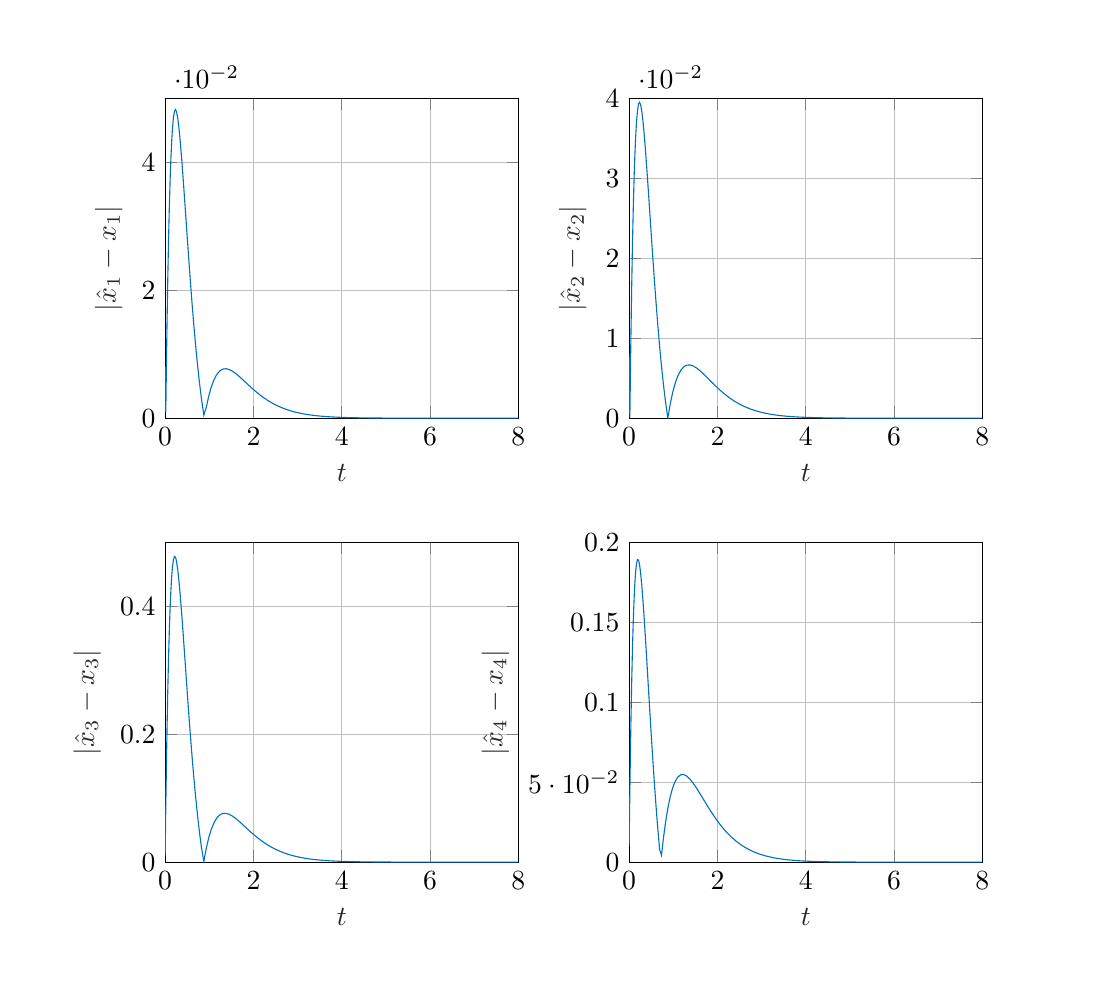
\begin{tikzpicture}

\begin{axis}[%
width=0.37\linewidth,
height=0.335\linewidth,
at={(0\linewidth,0.465\linewidth)},
scale only axis,
xmin=0,
xmax=8,
xlabel style={font=\color{white!15!black}},
xlabel={$t$},
ymin=0,
ymax=0.05,
ylabel style={font=\color{white!15!black}},
ylabel={$|\hat x_1 - x_1|$},
axis background/.style={fill=white},
xmajorgrids,
ymajorgrids
]
\addplot [color=mycolor1, forget plot]
  table[row sep=crcr]{%
0	0.008\\
0.000821791019927233	0.00747558057511985\\
0.00164358203985447	0.00695467686196013\\
0.0024653730597817	0.00643727196948394\\
0.00328716407970893	0.00592334907657911\\
0.0073961191793451	0.0034053804173415\\
0.0115050742789813	0.000971978655073036\\
0.0156140293786174	0.00137888127294253\\
0.0197229844782536	0.00364918329042435\\
0.0387608823959644	0.013172603109053\\
0.0577987803136751	0.0211887721439148\\
0.0768366782313859	0.0278622847742716\\
0.0958745761490967	0.033344115150995\\
0.113362875779606	0.0374469578210833\\
0.130851175410116	0.040753910932766\\
0.148339475040626	0.043351591908284\\
0.165827774671136	0.045319687606207\\
0.188844483406901	0.0470721653945121\\
0.211861192142666	0.0480043376567392\\
0.234877900878431	0.0482444397598385\\
0.257894609614196	0.0479077107018819\\
0.286451652811934	0.0468396713364636\\
0.315008696009671	0.0451980717902626\\
0.343565739207409	0.0431184698408835\\
0.372122782405147	0.0407201080479874\\
0.406266880391565	0.0375737020376313\\
0.440410978377984	0.0342409352955817\\
0.474555076364403	0.0308244873924237\\
0.508699174350821	0.0274130615643317\\
0.54279359208006	0.024080238579956\\
0.576888009809299	0.0208623159560511\\
0.610982427538538	0.0177921165859336\\
0.645076845267777	0.0148968107062984\\
0.689147209186533	0.0114442017559708\\
0.733217573105289	0.00832473706302984\\
0.777287937024045	0.00553763201510775\\
0.821358300942801	0.00308253960318246\\
0.876057604248058	0.000485714475901691\\
0.930756907553314	0.0016611603445986\\
0.98545621085857	0.00340674510198228\\
1.04015551416383	0.00478706866818899\\
1.10614002003457	0.00601891651312549\\
1.17212452590531	0.00686386807011577\\
1.23810903177604	0.00739663882154911\\
1.30409353764678	0.00767086414890954\\
1.37723575038186	0.00773093002395847\\
1.45037796311694	0.00760367602096879\\
1.52352017585202	0.0073418645726651\\
1.5966623885871	0.00698490097708599\\
1.6603502939681	0.0066214802789098\\
1.72403819934911	0.00622899297273501\\
1.78772610473011	0.00582108837248602\\
1.85141401011111	0.00540894354145407\\
1.92429316922088	0.00494337109190646\\
1.99717232833065	0.00449219941065011\\
2.07005148744042	0.00406140394053451\\
2.14293064655019	0.00365581345897748\\
2.23306543988133	0.0031938095022921\\
2.32320023321248	0.00277559589012667\\
2.41333502654363	0.00240012005418342\\
2.50346981987478	0.00206692864460389\\
2.61684746292718	0.00170580499060622\\
2.73022510597958	0.00140067771290625\\
2.84360274903198	0.0011436528267688\\
2.95698039208438	0.000929896657641329\\
3.07885390623398	0.000742832216158208\\
3.20072742038359	0.000591225075359742\\
3.3226009345332	0.000468545672132105\\
3.44447444868281	0.00037009747709204\\
3.55341378857437	0.000299289067376708\\
3.66235312846594	0.000241485930254552\\
3.7712924683575	0.000194417021153023\\
3.88023180824907	0.000156179210721828\\
4.00507089330387	0.000121146745935499\\
4.12990997835866	9.36841578491089e-05\\
4.25474906341346	7.2260004870124e-05\\
4.37958814846826	5.55520946769273e-05\\
4.50120601686873	4.27923315184323e-05\\
4.62282388526921	3.28254628506404e-05\\
4.74444175366968	2.50889448925387e-05\\
4.86605962207016	1.90770060063648e-05\\
5.0056119686397	1.37773877180924e-05\\
5.14516431520924	9.84141403158768e-06\\
5.28471666177879	6.96347740359801e-06\\
5.42426900834833	4.84958103857307e-06\\
5.62426900834833	2.67377766382561e-06\\
5.82426900834833	1.31675337232732e-06\\
6.02426900834833	5.88995435203167e-07\\
6.22426900834833	1.80867287744458e-07\\
6.41908266404877	1.14679667271309e-07\\
6.61389631974921	2.73763490373858e-07\\
6.80870997544965	3.3203741256157e-07\\
7.00352363115009	3.41158447984499e-07\\
7.2011139861915	3.36201907323087e-07\\
7.39870434123291	3.14344501991886e-07\\
7.59629469627431	2.82545313373391e-07\\
7.79388505131572	2.47630944105704e-07\\
7.84541378848679	2.38761184712707e-07\\
7.89694252565786	2.30019338993829e-07\\
7.94847126282893	2.21424595772993e-07\\
8	2.12993166192764e-07\\
};
\end{axis}

\begin{axis}[%
width=0.37\linewidth,
height=0.335\linewidth,
at={(0.486\linewidth,0.465\linewidth)},
scale only axis,
xmin=0,
xmax=8,
xlabel style={font=\color{white!15!black}},
xlabel={$t$},
ymin=0,
ymax=0.04,
ylabel style={font=\color{white!15!black}},
ylabel={$|\hat x_2 - x_2|$},
axis background/.style={fill=white},
xmajorgrids,
ymajorgrids
]
\addplot [color=mycolor1, forget plot]
  table[row sep=crcr]{%
0	0.008\\
0.000821791019927233	0.00755868305611477\\
0.00164358203985447	0.00712031858776661\\
0.0024653730597817	0.00668489240872701\\
0.00328716407970893	0.00625239039150928\\
0.0073961191793451	0.00413325209347357\\
0.0115050742789813	0.00208513238336095\\
0.0156140293786174	0.000106330494362235\\
0.0197229844782536	0.00180481978172862\\
0.0387608823959644	0.00982368719398547\\
0.0577987803136751	0.0165767940441004\\
0.0768366782313859	0.0222023700711103\\
0.0958745761490967	0.026827205191945\\
0.113362875779606	0.0302922704260999\\
0.130851175410116	0.0330889715524895\\
0.148339475040626	0.0352900449631771\\
0.165827774671136	0.0369624056479652\\
0.188844483406901	0.038459878989798\\
0.211861192142666	0.0392684469944574\\
0.234877900878431	0.0394957761572214\\
0.257894609614196	0.0392386166476268\\
0.286451652811934	0.0383733345358889\\
0.315008696009671	0.0370261652632917\\
0.343565739207409	0.0353108863998376\\
0.372122782405147	0.0333275768941132\\
0.406266880391565	0.0307215702585462\\
0.440410978377984	0.0279583997016666\\
0.474555076364403	0.0251242146713245\\
0.508699174350821	0.0222934442419039\\
0.54279359208006	0.0195277836276407\\
0.576888009809299	0.0168577261223635\\
0.610982427538538	0.0143108092393852\\
0.645076845267777	0.0119098346211766\\
0.689147209186533	0.00904836753295819\\
0.733217573105289	0.00646509745734326\\
0.777287937024045	0.00415936956055667\\
0.821358300942801	0.00213090454901921\\
0.876057604248058	1.07003320959712e-05\\
0.930756907553314	0.00177679220168944\\
0.98545621085857	0.00320820399316303\\
1.04015551416383	0.00433515908279829\\
1.10614002003457	0.00533376724760865\\
1.17212452590531	0.00601064422461902\\
1.23810903177604	0.00642841763137382\\
1.30409353764678	0.00663199629917282\\
1.37723575038186	0.00665606433137958\\
1.45037796311694	0.00652597463930892\\
1.52352017585202	0.00628576595750174\\
1.5966623885871	0.0059682613139876\\
1.6603502939681	0.00564954263418937\\
1.72403819934911	0.00530801151189876\\
1.78772610473011	0.00495496391567372\\
1.85141401011111	0.00459963253022182\\
1.92429316922088	0.00419948779145543\\
1.99717232833065	0.00381272896246836\\
2.07005148744042	0.00344420207106443\\
2.14293064655019	0.00309781184499004\\
2.23306543988133	0.00270382392317974\\
2.32320023321248	0.00234768153696581\\
2.41333502654363	0.00202832265610999\\
2.50346981987478	0.00174521651085432\\
2.61684746292718	0.0014386650451803\\
2.73022510597958	0.00117991866470988\\
2.84360274903198	0.000962189410461969\\
2.95698039208438	0.000781282595023807\\
3.07885390623398	0.000623103059797358\\
3.20072742038359	0.000495039985479831\\
3.3226009345332	0.000391532429825581\\
3.44447444868281	0.000308566560035552\\
3.55341378857437	0.000248960861193707\\
3.66235312846594	0.000200363137768721\\
3.7712924683575	0.000160844948010543\\
3.88023180824907	0.000128788973978505\\
4.00507089330387	9.94698950908496e-05\\
4.12990997835866	7.6535179366074e-05\\
4.25474906341346	5.86881689063124e-05\\
4.37958814846826	4.4808481217338e-05\\
4.50120601686873	3.42399111734307e-05\\
4.62282388526921	2.60138222856283e-05\\
4.74444175366968	1.96555399542502e-05\\
4.86605962207016	1.47381133410207e-05\\
5.0056119686397	1.04272311764908e-05\\
5.14516431520924	7.24998823185526e-06\\
5.28471666177879	4.94996070368454e-06\\
5.42426900834833	3.28012361976138e-06\\
5.62426900834833	1.58416196397349e-06\\
5.82426900834833	5.5608891037296e-07\\
6.02426900834833	3.9883971585347e-08\\
6.22426900834833	2.2334663276973e-07\\
6.41908266404877	4.07662176404866e-07\\
6.61389631974921	4.87866933384967e-07\\
6.80870997544965	4.92195348029034e-07\\
7.00352363115009	4.62775857235564e-07\\
7.2011139861915	4.27552797846724e-07\\
7.39870434123291	3.83527790657871e-07\\
7.59629469627431	3.35634174211967e-07\\
7.79388505131572	2.88843916001244e-07\\
7.84541378848679	2.77370545817551e-07\\
7.89694252565786	2.66203077520227e-07\\
7.94847126282893	2.55348015274588e-07\\
8	2.44809792219601e-07\\
};
\end{axis}

\begin{axis}[%
width=0.37\linewidth,
height=0.335\linewidth,
at={(0\linewidth,0\linewidth)},
scale only axis,
xmin=0,
xmax=8,
xlabel style={font=\color{white!15!black}},
xlabel={$t$},
ymin=0,
ymax=0.5,
ylabel style={font=\color{white!15!black}},
ylabel={$|\hat x_3 - x_3|$},
axis background/.style={fill=white},
xmajorgrids,
ymajorgrids
]
\addplot [color=mycolor1, forget plot]
  table[row sep=crcr]{%
0	0.01\\
0.000821791019927233	0.0145875789094434\\
0.00164358203985447	0.0191432699821076\\
0.0024653730597817	0.0236672282863375\\
0.00328716407970893	0.0281596082447624\\
0.0073961191793451	0.0501531956301857\\
0.0115050742789813	0.0713801177031084\\
0.0156140293786174	0.091858960951106\\
0.0197229844782536	0.111607932045819\\
0.0387608823959644	0.194097250213878\\
0.0577987803136751	0.262955526116733\\
0.0768366782313859	0.319691493985333\\
0.0958745761490967	0.365688312737222\\
0.113362875779606	0.399551939834962\\
0.130851175410116	0.426272419315871\\
0.148339475040626	0.446641467369688\\
0.165827774671136	0.461386992702479\\
0.188844483406901	0.473334560165795\\
0.211861192142666	0.478006020566962\\
0.234877900878431	0.476568853373477\\
0.257894609614196	0.470071202493395\\
0.286451652811934	0.456351757045717\\
0.315008696009671	0.437693755947362\\
0.343565739207409	0.4153223220767\\
0.372122782405147	0.390313502953842\\
0.406266880391565	0.358206056679734\\
0.440410978377984	0.324743811100545\\
0.474555076364403	0.290839946022577\\
0.508699174350821	0.257281316380543\\
0.54279359208006	0.224720096186102\\
0.576888009809299	0.193461124790472\\
0.610982427538538	0.163782621772029\\
0.645076845267777	0.13591265422343\\
0.689147209186533	0.102817574650047\\
0.733217573105289	0.0730473907055632\\
0.777287937024045	0.0465593670342688\\
0.821358300942801	0.0233186397638218\\
0.876057604248058	0.00115774864956708\\
0.930756907553314	0.0212870136557141\\
0.98545621085857	0.0375562541549191\\
1.04015551416383	0.0503310671723698\\
1.10614002003457	0.061618267617583\\
1.17212452590531	0.0692323656229096\\
1.23810903177604	0.0738925374572839\\
1.30409353764678	0.0761194384843941\\
1.37723575038186	0.0763062608629052\\
1.45037796311694	0.0747479477929009\\
1.52352017585202	0.071944488797471\\
1.5966623885871	0.0682712113638938\\
1.6603502939681	0.0646006331593477\\
1.72403819934911	0.0606763530192514\\
1.78772610473011	0.05662613360904\\
1.85141401011111	0.0525546387523183\\
1.92429316922088	0.0479744103789375\\
1.99717232833065	0.0435510608380709\\
2.07005148744042	0.039338947987157\\
2.14293064655019	0.0353819930395742\\
2.23306543988133	0.0308835965811575\\
2.32320023321248	0.0268190519373158\\
2.41333502654363	0.0231755024754522\\
2.50346981987478	0.0199463772851283\\
2.61684746292718	0.0164504693210613\\
2.73022510597958	0.0135000182275106\\
2.84360274903198	0.0110173049732393\\
2.95698039208438	0.00895422040494354\\
3.07885390623398	0.00714977318601318\\
3.20072742038359	0.00568829496485007\\
3.3226009345332	0.0045064701648535\\
3.44447444868281	0.00355853385251792\\
3.55341378857437	0.00287690038139543\\
3.66235312846594	0.00232064988143471\\
3.7712924683575	0.00186785673792811\\
3.88023180824907	0.00150011998596833\\
4.00507089330387	0.00116327337244776\\
4.12990997835866	0.000899288803242748\\
4.25474906341346	0.000693418935171997\\
4.37958814846826	0.000532910701715239\\
4.50120601686873	0.000410348778904113\\
4.62282388526921	0.000314638076702178\\
4.74444175366968	0.000240367805883157\\
4.86605962207016	0.000182669422683801\\
5.0056119686397	0.000131819058691085\\
5.14516431520924	9.40673123713265e-05\\
5.28471666177879	6.64777832493635e-05\\
5.42426900834833	4.62229611027931e-05\\
5.62426900834833	2.53823655038121e-05\\
5.82426900834833	1.23989321640372e-05\\
6.02426900834833	5.45605647941927e-06\\
6.22426900834833	1.57482745230531e-06\\
6.41908266404877	1.23703792348495e-06\\
6.61389631974921	2.74199991456836e-06\\
6.80870997544965	3.28090284995586e-06\\
7.00352363115009	3.35144651003594e-06\\
7.2011139861915	3.29142817159789e-06\\
7.39870434123291	3.07081675041121e-06\\
7.59629469627431	2.75552015865932e-06\\
7.79388505131572	2.4121603386662e-06\\
7.84541378848679	2.32537247352171e-06\\
7.89694252565786	2.23987545225346e-06\\
7.94847126282893	2.15585354576553e-06\\
8	2.07346225095106e-06\\
};
\end{axis}

\begin{axis}[%
width=0.37\linewidth,
height=0.335\linewidth,
at={(0.486\linewidth,0\linewidth)},
scale only axis,
xmin=0,
xmax=8,
xlabel style={font=\color{white!15!black}},
xlabel={$t$},
ymin=0,
ymax=0.2,
ylabel style={font=\color{white!15!black}},
ylabel={$|\hat x_4 - x_4|$},
axis background/.style={fill=white},
xmajorgrids,
ymajorgrids
]
\addplot [color=mycolor1, forget plot]
  table[row sep=crcr]{%
0	0.01\\
0.000821791019927233	0.0118993594579105\\
0.00164358203985447	0.0137846834973667\\
0.0024653730597817	0.015656042402334\\
0.00328716407970893	0.017513506159204\\
0.0073961191793451	0.0265948279007764\\
0.0115050742789813	0.0353390983637197\\
0.0156140293786174	0.043754735772762\\
0.0197229844782536	0.0518499834313126\\
0.0387608823959644	0.0854080453929955\\
0.0577987803136751	0.113009361454668\\
0.0768366782313859	0.135334748174493\\
0.0958745761490967	0.153007438672455\\
0.113362875779606	0.165624712081038\\
0.130851175410116	0.175177706041179\\
0.148339475040626	0.182020824450134\\
0.165827774671136	0.186479339260184\\
0.188844483406901	0.189208463740393\\
0.211861192142666	0.188903730888778\\
0.234877900878431	0.186081980099962\\
0.257894609614196	0.181206008687874\\
0.286451652811934	0.172906271445315\\
0.315008696009671	0.162693334597063\\
0.343565739207409	0.151098614843494\\
0.372122782405147	0.138587021515251\\
0.406266880391565	0.12296256138341\\
0.440410978377984	0.107053190877184\\
0.474555076364403	0.0912376017911624\\
0.508699174350821	0.0758399807108271\\
0.54279359208006	0.0611253225964576\\
0.576888009809299	0.0472025156761773\\
0.610982427538538	0.034171285985687\\
0.645076845267777	0.0221109481987258\\
0.689147209186533	0.00803797176187593\\
0.733217573105289	0.00435512446474862\\
0.777287937024045	0.0151255570907105\\
0.821358300942801	0.0243220984633675\\
0.876057604248058	0.0336571549210531\\
0.930756907553314	0.040954536480475\\
0.98545621085857	0.0464726119849359\\
1.04015551416383	0.0504082591938422\\
1.10614002003457	0.0533245462391934\\
1.17212452590531	0.0546451916565971\\
1.23810903177604	0.0547182392240927\\
1.30409353764678	0.0537970506159722\\
1.37723575038186	0.0518826059270603\\
1.45037796311694	0.0493283458362961\\
1.52352017585202	0.04636071433755\\
1.5966623885871	0.0431490585861365\\
1.6603502939681	0.0402579839317912\\
1.72403819934911	0.0373566427484852\\
1.78772610473011	0.0344971004324089\\
1.85141401011111	0.0317212258436821\\
1.92429316922088	0.0286875067364593\\
1.99717232833065	0.0258294119977292\\
2.07005148744042	0.0231620788547866\\
2.14293064655019	0.0206969269404987\\
2.23306543988133	0.0179350406091653\\
2.32320023321248	0.0154742577241497\\
2.41333502654363	0.013294910564105\\
2.50346981987478	0.0113823270961798\\
2.61684746292718	0.00932902728495094\\
2.73022510597958	0.00761191351817633\\
2.84360274903198	0.00617972830346472\\
2.95698039208438	0.00499762371743503\\
3.07885390623398	0.00396841616240151\\
3.20072742038359	0.00313973304582144\\
3.3226009345332	0.00247389152275118\\
3.44447444868281	0.00194249073768285\\
3.55341378857437	0.00156156856092902\\
3.66235312846594	0.00125202440688894\\
3.7712924683575	0.00100120616537572\\
3.88023180824907	0.000798371342467186\\
4.00507089330387	0.000613314374967255\\
4.12990997835866	0.000469070799417839\\
4.25474906341346	0.000357305265157981\\
4.37958814846826	0.000270720844733147\\
4.50120601686873	0.000204994460160077\\
4.62282388526921	0.000154061911922992\\
4.74444175366968	0.000114903875506125\\
4.86605962207016	8.47870284098884e-05\\
5.0056119686397	5.85365180337388e-05\\
5.14516431520924	3.93551584345619e-05\\
5.28471666177879	2.56303498849808e-05\\
5.42426900834833	1.57959966571378e-05\\
5.62426900834833	5.94303198957896e-06\\
5.82426900834833	1.68178369060884e-07\\
6.02426900834833	2.48040614337502e-06\\
6.22426900834833	3.64047919205329e-06\\
6.41908266404877	4.41802235401356e-06\\
6.61389631974921	4.6026881795995e-06\\
6.80870997544965	4.35861497611809e-06\\
7.00352363115009	3.94940252674419e-06\\
7.2011139861915	3.54632716900727e-06\\
7.39870434123291	3.11836929831055e-06\\
7.59629469627431	2.68937443886202e-06\\
7.79388505131572	2.29025674083894e-06\\
7.84541378848679	2.19473025781999e-06\\
7.89694252565786	2.10223442165258e-06\\
7.94847126282893	2.01276527397529e-06\\
8	1.92630733113555e-06\\
};
\end{axis}

\begin{axis}[%
width=1.104\linewidth,
height=0.982\linewidth,
at={(-0.144\linewidth,-0.108\linewidth)},
scale only axis,
xmin=0,
xmax=1,
ymin=0,
ymax=1,
axis line style={draw=none},
ticks=none,
axis x line*=bottom,
axis y line*=left
]
\end{axis}
\end{tikzpicture}%
	\caption{Абсолютное отклонение оценки от настоящего состояния линейной системы для предыдущей задачи.}
\end{figure}

\begin{figure}[t]
	\centering
	% This file was created by matlab2tikz.
%
%The latest updates can be retrieved from
%  http://www.mathworks.com/matlabcentral/fileexchange/22022-matlab2tikz-matlab2tikz
%where you can also make suggestions and rate matlab2tikz.
%
\definecolor{mycolor1}{rgb}{0.00000,0.44700,0.74100}%
%
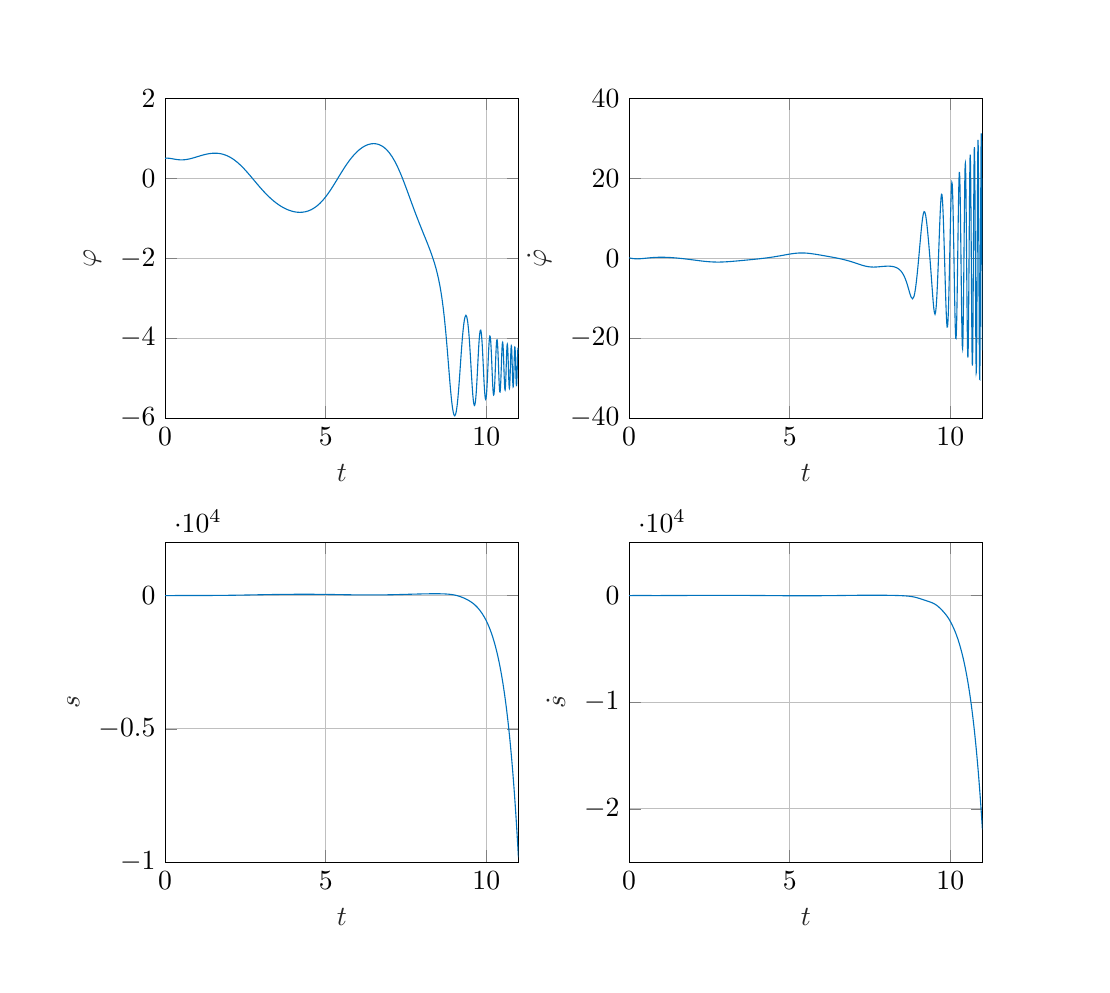
\begin{tikzpicture}

\begin{axis}[%
width=0.37\linewidth,
height=0.335\linewidth,
at={(0\linewidth,0.465\linewidth)},
scale only axis,
xmin=0,
xmax=11,
xlabel style={font=\color{white!15!black}},
xlabel={$t$},
ymin=-6,
ymax=2,
ylabel style={font=\color{white!15!black}},
ylabel={$\varphi$},
axis background/.style={fill=white},
xmajorgrids,
ymajorgrids
]
\addplot [color=mycolor1, forget plot]
  table[row sep=crcr]{%
0	0.5\\
0.000178417029156271	0.500017812311672\\
0.000356834058312542	0.500035565853097\\
0.000535251087468813	0.500053260642706\\
0.000713668116625084	0.500070896699033\\
0.00160575326240644	0.500158196636744\\
0.0024978384081878	0.500244031079346\\
0.00338992355396915	0.50032840245441\\
0.00428200869975051	0.500411313249568\\
0.00874243442865728	0.500804048881674\\
0.0132028601575641	0.501160677372609\\
0.0176632858864708	0.501481574547605\\
0.0221237116153776	0.501767147154384\\
0.0379624479282651	0.502502054961113\\
0.0538011842411526	0.502820102721187\\
0.0696399205540401	0.502747872625998\\
0.0854786568669277	0.502313363863655\\
0.104518190123929	0.501353863596216\\
0.123557723380931	0.499972427028462\\
0.142597256637933	0.498227899869598\\
0.161636789894934	0.496177129747661\\
0.184754110311784	0.493356169623264\\
0.207871430728634	0.490270383480711\\
0.230988751145485	0.487017694980061\\
0.254106071562335	0.483686437707419\\
0.280545594271983	0.479885007014582\\
0.306985116981632	0.476205612801324\\
0.33342463969128	0.472751114306403\\
0.359864162400929	0.469607680791091\\
0.389966777126792	0.466500414576392\\
0.420069391852654	0.463983838285225\\
0.450172006578517	0.46212840441704\\
0.48027462130438	0.460983701411856\\
0.514678811154934	0.460586762383712\\
0.549083001005487	0.461182533541759\\
0.583487190856041	0.462768879475327\\
0.617891380706595	0.465324446937716\\
0.663023553466504	0.470082527422204\\
0.708155726226414	0.476306424703572\\
0.753287898986323	0.483829999531182\\
0.798420071746233	0.492476150662047\\
0.859301430150392	0.505587473827881\\
0.920182788554552	0.51986013865209\\
0.981064146958711	0.534762533934377\\
1.04194550536287	0.549828408996633\\
1.09747200573599	0.563336396423564\\
1.1529985061091	0.576257478044053\\
1.20852500648222	0.588280783310938\\
1.26405150685533	0.599132897702174\\
1.32673314109095	0.609662794991131\\
1.38941477532657	0.618038914056966\\
1.45209640956219	0.623958400746614\\
1.51477804379781	0.627153145029245\\
1.58476498039001	0.627199178979856\\
1.65475191698221	0.623227868660833\\
1.72473885357441	0.614963137599296\\
1.79472579016661	0.602156264908731\\
1.88480308448625	0.5786442672722\\
1.97488037880589	0.546899177151692\\
2.06495767312553	0.506717780738717\\
2.15503496744517	0.45806051549702\\
2.25693032557634	0.39312472199534\\
2.35882568370751	0.318284144286231\\
2.46072104183868	0.234660566831558\\
2.56261639996985	0.144152447810348\\
2.64825924393788	0.0644307328026832\\
2.73390208790591	-0.0172622732634186\\
2.81954493187395	-0.0994969910925584\\
2.90518777584198	-0.180801883842625\\
2.9817967362064	-0.251693275425333\\
3.05840569657082	-0.320098178995783\\
3.13501465693524	-0.385370527582576\\
3.21162361729966	-0.447083118807643\\
3.29545204705276	-0.510193616172889\\
3.37928047680587	-0.56833866493317\\
3.46310890655897	-0.621320297608046\\
3.54693733631208	-0.669110680371053\\
3.62177085401317	-0.707359256601047\\
3.69660437171426	-0.741338313917257\\
3.77143788941536	-0.771003082518281\\
3.84627140711645	-0.796282514764363\\
3.93186166883489	-0.819679072980819\\
4.01745193055334	-0.836973981155806\\
4.10304219227178	-0.847891004375819\\
4.18863245399022	-0.852092292366984\\
4.27722667424324	-0.848913967870243\\
4.36582089449626	-0.837516082023049\\
4.45441511474929	-0.817285620308174\\
4.54300933500231	-0.787556007670131\\
4.63637531273009	-0.745212848422824\\
4.72974129045787	-0.690808991249897\\
4.82310726818565	-0.623810078177168\\
4.91647324591343	-0.544056176562243\\
4.9867668823177	-0.475787949418582\\
5.05706051872197	-0.400867828063416\\
5.12735415512623	-0.319940044753792\\
5.1976477915305	-0.234004714335025\\
5.26794142793477	-0.144310867694967\\
5.33823506433903	-0.0521981140426555\\
5.4085287007433	0.0408376770279202\\
5.47882233714757	0.133176668821844\\
5.54353212614873	0.216250571460007\\
5.60824191514989	0.296438908900647\\
5.67295170415105	0.372834454550514\\
5.73766149315221	0.444756525777852\\
5.79544944089558	0.50479407442851\\
5.85323738863896	0.560573233856685\\
5.91102533638233	0.611901622528733\\
5.9688132841257	0.658680422235664\\
6.02660123186907	0.700853302585848\\
6.08438917961245	0.738364389320157\\
6.14217712735582	0.771185210972349\\
6.19996507509919	0.799286616143524\\
6.25899708510857	0.823070206105504\\
6.31802909511794	0.84180048001971\\
6.37706110512732	0.855370508855036\\
6.4360931151367	0.863628720691722\\
6.4959639126223	0.866375495110404\\
6.55583471010791	0.863199594710789\\
6.61570550759352	0.853793517856003\\
6.67557630507913	0.837794826251093\\
6.75036650325845	0.807923369885787\\
6.82515670143776	0.766207950384744\\
6.89994689961708	0.711698824075273\\
6.9747370977964	0.64346705631141\\
7.06501876282321	0.541827932668028\\
7.15530042785002	0.418103309004707\\
7.24558209287683	0.272460445948869\\
7.33586375790364	0.106963308727197\\
7.39427829276798	-0.00901863744622682\\
7.45269282763233	-0.130549022433152\\
7.51110736249667	-0.256154065950326\\
7.56952189736102	-0.384217775088088\\
7.62793643222536	-0.513180087234119\\
7.68635096708971	-0.641733587725985\\
7.74476550195406	-0.768815775120681\\
7.8031800368184	-0.893739053324053\\
7.85180853748465	-0.995839506613675\\
7.9004370381509	-1.09618174596384\\
7.94906553881715	-1.19490622270347\\
7.99769403948341	-1.29232363837366\\
8.04632254014966	-1.38890586629983\\
8.09495104081591	-1.48524306133496\\
8.14357954148216	-1.58213363034556\\
8.19220804214841	-1.6806194406979\\
8.23982768556392	-1.77989577267596\\
8.28744732897943	-1.88352827389158\\
8.33506697239495	-1.99357716906112\\
8.38268661581046	-2.11274918914269\\
8.42538992081576	-2.23021685663976\\
8.46809322582106	-2.36106735366143\\
8.51079653082637	-2.50947866346887\\
8.55349983583167	-2.68065187566554\\
8.59010254804154	-2.8500941244271\\
8.62670526025141	-3.04574067357283\\
8.66330797246128	-3.27248710854999\\
8.69991068467115	-3.53439790248116\\
8.74198281523799	-3.88181951896381\\
8.78405494580482	-4.27529975760892\\
8.82612707637166	-4.69790678160018\\
8.86819920693849	-5.11740179332948\\
8.89325396451413	-5.34755498717619\\
8.91830872208976	-5.55088614527096\\
8.9433634796654	-5.71844636080028\\
8.96841823724103	-5.8427630606341\\
8.99347299481667	-5.9182749851325\\
9.0185277523923	-5.94068191846903\\
9.04358250996794	-5.90710103083158\\
9.06863726754357	-5.81677072885489\\
9.09150541010144	-5.68579252830983\\
9.1143735526593	-5.51109285833704\\
9.13724169521716	-5.29808765965698\\
9.16010983777503	-5.05531584648171\\
9.18454580457801	-4.7757473300695\\
9.20898177138098	-4.49134840937593\\
9.23341773818396	-4.21824659749237\\
9.25785370498694	-3.97123575546667\\
9.27786902154505	-3.79697248822732\\
9.29788433810317	-3.65275691836562\\
9.31789965466128	-3.54217362073036\\
9.33791497121939	-3.46793085837312\\
9.36592131740018	-3.42835247885277\\
9.39392766358096	-3.46941337340128\\
9.42193400976174	-3.59573455586091\\
9.44994035594253	-3.80851659519519\\
9.46840810140955	-3.99462299159039\\
9.48687584687657	-4.21283756887321\\
9.5053435923436	-4.45575704757208\\
9.52381133781062	-4.71224457983741\\
9.54227908327764	-4.96804536281427\\
9.56074682874467	-5.206235417242\\
9.57921457421169	-5.4102078635959\\
9.59768231967871	-5.56513436797402\\
9.61281558675494	-5.64720577203389\\
9.62794885383117	-5.68362536635685\\
9.64308212090741	-5.67092205188223\\
9.65821538798364	-5.6078966017254\\
9.67172151679969	-5.5098396828966\\
9.68522764561573	-5.37433693704592\\
9.69873377443178	-5.205739260735\\
9.71223990324783	-5.0110807682135\\
9.72596837154835	-4.79613173444352\\
9.73969683984887	-4.5760540823975\\
9.7534253081494	-4.36368645169778\\
9.76715377644992	-4.17161776539747\\
9.7788444151093	-4.03260264881213\\
9.79053505376869	-3.92201308837136\\
9.80222569242807	-3.84425969227074\\
9.81391633108746	-3.80230307562519\\
9.82640226791932	-3.79883450619691\\
9.83888820475118	-3.83932245747677\\
9.85137414158304	-3.92337732566354\\
9.86386007841491	-4.04841482214267\\
9.87634601524677	-4.20978431609382\\
9.88883195207863	-4.4002781146275\\
9.90131788891049	-4.60982623276856\\
9.91380382574235	-4.82568656601266\\
9.92479235693768	-5.00950971603185\\
9.935780888133	-5.17725982219455\\
9.94676941932833	-5.31976356931548\\
9.95775795052366	-5.42935737680932\\
9.96885634060718	-5.50074459414137\\
9.9799547306907	-5.5279095799569\\
9.99105312077422	-5.50803697831315\\
10.0021515108577	-5.44106638498281\\
10.0113218641467	-5.35178188828495\\
10.0204922174357	-5.23427944437077\\
10.0296625707246	-5.09265650375151\\
10.0388329240136	-4.93273919033577\\
10.0482913340798	-4.75627946579353\\
10.057749744146	-4.57737228794459\\
10.0672081542122	-4.4057303438513\\
10.0766665642784	-4.25077786905039\\
10.0853090499258	-4.1310426426868\\
10.0939515355732	-4.03778986497713\\
10.1025940212205	-3.97532782173347\\
10.1112365068679	-3.94642809060883\\
10.1197040637527	-3.95199355202996\\
10.1281716206375	-3.99167176146214\\
10.1366391775224	-4.06463387983665\\
10.1451067344072	-4.16836041736198\\
10.153574291292	-4.29883420053723\\
10.1620418481768	-4.45042786799184\\
10.1705094050616	-4.61587377303052\\
10.1789769619464	-4.78648441954811\\
10.1869187532118	-4.94276080153693\\
10.1948605444772	-5.08732674355815\\
10.2028023357426	-5.21281106484088\\
10.2107441270079	-5.31297991565937\\
10.2191985710553	-5.38639779158606\\
10.2276530151027	-5.42098888272825\\
10.23610745915	-5.41396391674117\\
10.2445619031974	-5.36513697445385\\
10.2517272557398	-5.29246888840646\\
10.2588926082823	-5.19335750865476\\
10.2660579608247	-5.07150191053722\\
10.2732233133671	-4.93213585313247\\
10.2803885115728	-4.7816995285926\\
10.2875537097786	-4.62769606891298\\
10.2947189079843	-4.47801821267269\\
10.30188410619	-4.3404308626717\\
10.3086771800465	-4.22767636745822\\
10.315470253903	-4.13757258031849\\
10.3222633277595	-4.07442005921288\\
10.3290564016159	-4.04108157704184\\
10.3357078300507	-4.03880975412562\\
10.3423592584854	-4.06729834262161\\
10.3490106869201	-4.12593524576386\\
10.3556621153548	-4.21254304863293\\
10.3623135437895	-4.32360248076689\\
10.3689649722242	-4.45428966676132\\
10.375616400659	-4.59839885673377\\
10.3822678290937	-4.74852771555643\\
10.3885422365267	-4.88840123053897\\
10.3948166439597	-5.0195219659186\\
10.4010910513927	-5.13536766394454\\
10.4073654588257	-5.23032492887898\\
10.4141373438571	-5.30425338344438\\
10.4209092288885	-5.34408773131354\\
10.4276811139198	-5.34699716474287\\
10.4344529989512	-5.31252026092355\\
10.4403982223182	-5.25260199913549\\
10.4463434456851	-5.16695877624973\\
10.4522886690521	-5.0589886167468\\
10.458233892419	-4.93357495135979\\
10.4639873072004	-4.8012689712809\\
10.4697407219818	-4.6645924327893\\
10.4754941367632	-4.53026201699049\\
10.4812475515446	-4.40495994588405\\
10.4868248410515	-4.29804467730989\\
10.4924021305584	-4.21063188658172\\
10.4979794200652	-4.14692394887428\\
10.5035567095721	-4.10981810763483\\
10.5090614718767	-4.1009171028877\\
10.5145662341812	-4.12043478139252\\
10.5200709964857	-4.16799679062909\\
10.5255757587903	-4.24174459851676\\
10.5310805210948	-4.33857056699581\\
10.5365852833993	-4.45423905131971\\
10.5420900457039	-4.58326709805266\\
10.5475948080084	-4.71907938488603\\
10.552784804832	-4.84686571471783\\
10.5579748016555	-4.96806119354119\\
10.5631647984791	-5.07673791101184\\
10.5683547953027	-5.16770831835041\\
10.5739840151887	-5.24146940642673\\
10.5796132350746	-5.28497751355023\\
10.5852424549606	-5.29535705590895\\
10.5908716748466	-5.27188078266195\\
10.5959961609566	-5.22195961239863\\
10.6011206470666	-5.14658171807093\\
10.6062451331767	-5.04891301253129\\
10.6113696192867	-4.93362206472417\\
10.6161727436816	-4.81471218794879\\
10.6209758680764	-4.69092257440934\\
10.6257789924713	-4.56815295444334\\
10.6305821168662	-4.45232452117286\\
10.6353031206321	-4.3506936882083\\
10.6400241243979	-4.26608168001384\\
10.6447451281637	-4.20255070457255\\
10.6494661319295	-4.1629845089208\\
10.6541437585173	-4.14915367865584\\
10.6588213851051	-4.16158832334746\\
10.6634990116929	-4.2001293756776\\
10.6681766382807	-4.26323082203934\\
10.6728542648684	-4.34818948479965\\
10.6775318914562	-4.45131159805068\\
10.682209518044	-4.56776641169207\\
10.6868871446318	-4.69171164980418\\
10.6913135199586	-4.8100682124317\\
10.6957398952855	-4.92368286534237\\
10.7001662706123	-5.02707184711481\\
10.7045926459392	-5.11535122268442\\
10.7093850247391	-5.18919260845938\\
10.714177403539	-5.23620178874385\\
10.7189697823389	-5.25344705953338\\
10.7237621611388	-5.23992090728201\\
10.7283188423865	-5.19908998431\\
10.7328755236342	-5.13248018399578\\
10.7374322048819	-5.0430575032763\\
10.7419888861296	-4.93538410352072\\
10.746111143448	-4.82703594117856\\
10.7502334007663	-4.7133401489651\\
10.7543556580847	-4.59959006689094\\
10.7584779154031	-4.49114618286894\\
10.7625609208143	-4.39402554368967\\
10.7666439262255	-4.31179984436956\\
10.7707269316367	-4.2483889183934\\
10.7748099370479	-4.20665464194666\\
10.778886742879	-4.18844749776328\\
10.7829635487101	-4.19483743270666\\
10.7870403545412	-4.225869272823\\
10.7911171603724	-4.28026734589291\\
10.7951939662035	-4.35565943127809\\
10.7992707720346	-4.44877424842319\\
10.8033475778657	-4.55527301201631\\
10.8074243836968	-4.66985140405523\\
10.8112805138584	-4.78033567216305\\
10.81513664402	-4.88754410456866\\
10.8189927741816	-4.98636591041615\\
10.8228489043432	-5.0721776965627\\
10.8270129984041	-5.14570949325926\\
10.8311770924651	-5.19524715546445\\
10.8353411865261	-5.2178272599585\\
10.839505280587	-5.21221917016225\\
10.8436367957204	-5.17906964107446\\
10.8477683108537	-5.11967446038494\\
10.8518998259871	-5.03683058450526\\
10.8560313411205	-4.93505837934267\\
10.8596434549192	-4.83509614483872\\
10.863255568718	-4.72949985732315\\
10.8668676825167	-4.62310307186017\\
10.8704797963155	-4.52083537103101\\
10.8740942171358	-4.42741302494075\\
10.8777086379562	-4.34738804281895\\
10.8813230587766	-4.28459076255584\\
10.8849374795969	-4.24187009248064\\
10.8885553059354	-4.22110840864981\\
10.8921731322739	-4.22359270494522\\
10.8957909586124	-4.24949957276407\\
10.899408784951	-4.29773522756678\\
10.9030266112895	-4.36615457029389\\
10.906644437628	-4.45177740687602\\
10.9102622639665	-4.55061171367858\\
10.913880090305	-4.65774171423045\\
10.9172939912164	-4.76150229163268\\
10.9207078921277	-4.86290823853825\\
10.9241217930391	-4.95717880632512\\
10.9275356939505	-5.03994522028638\\
10.9312247138177	-5.11211291459635\\
10.9349137336849	-5.16233920142781\\
10.9386027535521	-5.18768354857254\\
10.9422917734193	-5.18680456277807\\
10.9460611650798	-5.15890096253846\\
10.9498305567403	-5.10475144453795\\
10.9535999484008	-5.02701898214524\\
10.9573693400613	-4.9301699789569\\
10.9605851421966	-4.83675344047029\\
10.9638009443319	-4.73768997337671\\
10.9670167464673	-4.63746206757582\\
10.9702325486026	-4.54065672553618\\
10.9734733723346	-4.4510827874232\\
10.9767141960666	-4.37382450414194\\
10.9799550197986	-4.31258733174816\\
10.9831958435306	-4.27015723759875\\
10.9862901814175	-4.2489471586234\\
10.9893845193044	-4.24771681041635\\
10.9924788571913	-4.26672590956193\\
10.9955731950782	-4.3052468841433\\
10.9966798963086	-4.32348093932137\\
10.9977865975391	-4.34393585420835\\
10.9988932987695	-4.3665051967409\\
11	-4.39106953738969\\
};
\end{axis}

\begin{axis}[%
width=0.37\linewidth,
height=0.335\linewidth,
at={(0.486\linewidth,0.465\linewidth)},
scale only axis,
xmin=0,
xmax=11,
xlabel style={font=\color{white!15!black}},
xlabel={$t$},
ymin=-40,
ymax=40,
ylabel style={font=\color{white!15!black}},
ylabel={$\dot\varphi$},
axis background/.style={fill=white},
xmajorgrids,
ymajorgrids
]
\addplot [color=mycolor1, forget plot]
  table[row sep=crcr]{%
0	0.1\\
0.000178417029156271	0.0996705503328423\\
0.000356834058312542	0.0993412036981584\\
0.000535251087468813	0.0990119606555194\\
0.000713668116625084	0.0986828217632261\\
0.00160575326240644	0.0970387090106609\\
0.0024978384081878	0.09539728303225\\
0.00338992355396915	0.0937586121941229\\
0.00428200869975051	0.0921227640854385\\
0.00874243442865728	0.0839881826227258\\
0.0132028601575641	0.0759338641110729\\
0.0176632858864708	0.0679674066625221\\
0.0221237116153776	0.0600959756219243\\
0.0379624479282651	0.0330134048445082\\
0.0538011842411526	0.00746741095619446\\
0.0696399205540401	-0.0163426481320486\\
0.0854786568669277	-0.0382581521697989\\
0.104518190123929	-0.0619332606473484\\
0.123557723380931	-0.0826025938540807\\
0.142597256637933	-0.100222228798034\\
0.161636789894934	-0.114784426956302\\
0.184754110311784	-0.128408533823486\\
0.207871430728634	-0.137766425219861\\
0.230988751145485	-0.143092524383752\\
0.254106071562335	-0.144631583078483\\
0.280545594271983	-0.142104391415625\\
0.306985116981632	-0.135500714319694\\
0.33342463969128	-0.125333488579155\\
0.359864162400929	-0.112080330092599\\
0.389966777126792	-0.0938340885698942\\
0.420069391852654	-0.0729397770069257\\
0.450172006578517	-0.0500776773851494\\
0.48027462130438	-0.0258457318614439\\
0.514678811154934	0.00282486877551835\\
0.549083001005487	0.0317855683723616\\
0.583487190856041	0.0603675723348833\\
0.617891380706595	0.0880199775680299\\
0.663023553466504	0.122116740213741\\
0.708155726226414	0.152963923571984\\
0.753287898986323	0.179942461217295\\
0.798420071746233	0.202641806885604\\
0.859301430150392	0.226020665010289\\
0.920182788554552	0.240986108868637\\
0.981064146958711	0.247722227163541\\
1.04194550536287	0.246521079415629\\
1.09747200573599	0.238864696850682\\
1.1529985061091	0.225480574582108\\
1.20852500648222	0.206866643642156\\
1.26405150685533	0.183421334268112\\
1.32673314109095	0.15161170390202\\
1.38941477532657	0.114769222007634\\
1.45209640956219	0.0734276133476926\\
1.51477804379781	0.0279458109343494\\
1.58476498039001	-0.0273242416404413\\
1.65475191698221	-0.0867954039271939\\
1.72473885357441	-0.150007102145916\\
1.79472579016661	-0.216526287740795\\
1.88480308448625	-0.306089298707257\\
1.97488037880589	-0.398920320838674\\
2.06495767312553	-0.493345434635229\\
2.15503496744517	-0.586912326234886\\
2.25693032557634	-0.688567985149362\\
2.35882568370751	-0.780332464812223\\
2.46072104183868	-0.856612543129399\\
2.56261639996985	-0.913912112289752\\
2.64825924393788	-0.94575186101461\\
2.73390208790591	-0.960243005055364\\
2.81954493187395	-0.956900567928651\\
2.90518777584198	-0.938069952150761\\
2.9817967362064	-0.910308625027196\\
3.05840569657082	-0.873567219644222\\
3.13501465693524	-0.829975616272548\\
3.21162361729966	-0.781175303974515\\
3.29545204705276	-0.723144631214495\\
3.37928047680587	-0.662768620763154\\
3.46310890655897	-0.60170606599897\\
3.54693733631208	-0.539530722591593\\
3.62177085401317	-0.482655944161877\\
3.69660437171426	-0.425309845752052\\
3.77143788941536	-0.367321068286533\\
3.84627140711645	-0.3081040791712\\
3.93186166883489	-0.238091955388247\\
4.01745193055334	-0.165346912885962\\
4.10304219227178	-0.0891547545558693\\
4.18863245399022	-0.00835842494609285\\
4.27722667424324	0.0811497151694538\\
4.36582089449626	0.177255728902074\\
4.45441511474929	0.280682782639453\\
4.54300933500231	0.391840120272061\\
4.63637531273009	0.51695952354242\\
4.72974129045787	0.649203489720663\\
4.82310726818565	0.785928924585577\\
4.91647324591343	0.922082138794531\\
4.9867668823177	1.02026831830971\\
5.05706051872197	1.11059780057133\\
5.12735415512623	1.18899528840131\\
5.1976477915305	1.25212986855559\\
5.26794142793477	1.2972980735385\\
5.33823506433903	1.32105166220262\\
5.4085287007433	1.32171029448668\\
5.47882233714757	1.3005395579427\\
5.54353212614873	1.26372761904012\\
5.60824191514989	1.21195246044266\\
5.67295170415105	1.14787404384663\\
5.73766149315221	1.07425903976622\\
5.79544944089558	1.00253749242862\\
5.85323738863896	0.927047843392356\\
5.91102533638233	0.849278999337677\\
5.9688132841257	0.769960837684204\\
6.02660123186907	0.689505568292072\\
6.08438917961245	0.608554209277616\\
6.14217712735582	0.527254586390462\\
6.19996507509919	0.445279869235097\\
6.25899708510857	0.36035995092131\\
6.31802909511794	0.273922298550123\\
6.37706110512732	0.185355868849519\\
6.4360931151367	0.0938578686558413\\
6.4959639126223	-0.00279442057905675\\
6.55583471010791	-0.10414315468139\\
6.61570550759352	-0.211087823667447\\
6.67557630507913	-0.324524588371258\\
6.75036650325845	-0.476447063137592\\
6.82515670143776	-0.640998306648792\\
6.89994689961708	-0.818595890638833\\
6.9747370977964	-1.008120488404\\
7.06501876282321	-1.24912253781331\\
7.15530042785002	-1.49350257510385\\
7.24558209287683	-1.72641421214559\\
7.33586375790364	-1.93020487265196\\
7.39427829276798	-2.03762292844363\\
7.45269282763233	-2.12019217060935\\
7.51110736249667	-2.17530435299104\\
7.56952189736102	-2.20354103284662\\
7.62793643222536	-2.20741667949814\\
7.68635096708971	-2.1907064160073\\
7.74476550195406	-2.15879617388891\\
7.8031800368184	-2.11776660610503\\
7.85180853748465	-2.08118013882366\\
7.9004370381509	-2.04600261522268\\
7.94906553881715	-2.01554798487824\\
7.99769403948341	-1.99286454530036\\
8.04632254014966	-1.98114109800141\\
8.09495104081591	-1.98379140839398\\
8.14357954148216	-2.00495928837179\\
8.19220804214841	-2.05006495993927\\
8.23982768556392	-2.12422916134565\\
8.28744732897943	-2.23589408757973\\
8.33506697239495	-2.39616370472582\\
8.38268661581046	-2.62071371811451\\
8.42538992081576	-2.89340790913077\\
8.46809322582106	-3.2521299928324\\
8.51079653082637	-3.71914573381829\\
8.55349983583167	-4.32153053466132\\
8.59010254804154	-4.96569048166696\\
8.62670526025141	-5.74540239959789\\
8.66330797246128	-6.65740616497859\\
8.69991068467115	-7.66719193080742\\
8.74198281523799	-8.85479967215459\\
8.78405494580482	-9.79704438528944\\
8.82612707637166	-10.1525939516651\\
8.86819920693849	-9.58748687305489\\
8.89325396451413	-8.71393106268132\\
8.91830872208976	-7.46000200601503\\
8.9433634796654	-5.86941289946067\\
8.96841823724103	-4.01413453685594\\
8.99347299481667	-1.97135531085932\\
9.0185277523923	0.209226169717206\\
9.04358250996794	2.4664388727783\\
9.06863726754357	4.72678947829176\\
9.09150541010144	6.71705200947859\\
9.1143735526593	8.52747314981976\\
9.13724169521716	10.0335957352445\\
9.16010983777503	11.1083824000949\\
9.18454580457801	11.6580255012313\\
9.20898177138098	11.5258857893324\\
9.23341773818396	10.7300380294204\\
9.25785370498694	9.38647056370158\\
9.27786902154505	7.99011965105055\\
9.29788433810317	6.38931985716496\\
9.31789965466128	4.6360157210907\\
9.33791497121939	2.76732162372848\\
9.36592131740018	0.000257432249171075\\
9.39392766358096	-2.95616817007912\\
9.42193400976174	-6.05167226390822\\
9.44994035594253	-9.12498704960751\\
9.46840810140955	-11.0013263590704\\
9.48687584687657	-12.5688313101628\\
9.5053435923436	-13.6336128263203\\
9.52381133781062	-14.0041936791566\\
9.54227908327764	-13.5286611768347\\
9.56074682874467	-12.1313163691521\\
9.57921457421169	-9.83952108508689\\
9.59768231967871	-6.81758323198721\\
9.61281558675494	-3.94951438756904\\
9.62794885383117	-0.812101806387987\\
9.64308212090741	2.48627469149954\\
9.65821538798364	5.81621217714824\\
9.67172151679969	8.69341742520224\\
9.68522764561573	11.3269727920428\\
9.69873377443178	13.5417619353521\\
9.71223990324783	15.1541121991727\\
9.72596837154835	16.0012610200873\\
9.73969683984887	15.9205537278941\\
9.7534253081494	14.8751422790547\\
9.76715377644992	12.950121722741\\
9.7788444151093	10.7399750610251\\
9.79053505376869	8.10786405275894\\
9.80222569242807	5.16041770175277\\
9.81391633108746	2.0044972876124\\
9.82640226791932	-1.48782096572474\\
9.83888820475118	-5.00324591453814\\
9.85137414158304	-8.40890579018588\\
9.86386007841491	-11.5424827006993\\
9.87634601524677	-14.2171981622296\\
9.88883195207863	-16.1816978956136\\
9.90131788891049	-17.2095387856013\\
9.91380382574235	-17.1473751331886\\
9.92479235693768	-16.1367874064225\\
9.935780888133	-14.2539235934398\\
9.94676941932833	-11.5834026935194\\
9.95775795052366	-8.27788016902976\\
9.96885634060718	-4.47515133071631\\
9.9799547306907	-0.353936987917057\\
9.99105312077422	3.9058851664739\\
10.0021515108577	8.09585762538768\\
10.0113218641467	11.3419422095387\\
10.0204922174357	14.2196570556138\\
10.0296625707246	16.5538116469665\\
10.0388329240136	18.1770848853044\\
10.0482913340798	18.9551024170661\\
10.057749744146	18.7139264538156\\
10.0672081542122	17.4272956972523\\
10.0766665642784	15.1757473175495\\
10.0853090499258	12.4045967085334\\
10.0939515355732	9.07846254406645\\
10.1025940212205	5.33913658128357\\
10.1112365068679	1.33976420207111\\
10.1197040637527	-2.68685499158226\\
10.1281716206375	-6.68197160533618\\
10.1366391775224	-10.4847629783735\\
10.1451067344072	-13.9173856275892\\
10.153574291292	-16.791142392267\\
10.1620418481768	-18.8868843007654\\
10.1705094050616	-20.0190675841349\\
10.1789769619464	-20.0698058697716\\
10.1869187532118	-19.0941573243537\\
10.1948605444772	-17.1534556736025\\
10.2028023357426	-14.3351899317782\\
10.2107441270079	-10.7932197630035\\
10.2191985710553	-6.4341322809799\\
10.2276530151027	-1.66303521236261\\
10.23610745915	3.29217482102155\\
10.2445619031974	8.17783698296599\\
10.2517272557398	12.0662067947701\\
10.2588926082823	15.5247588850457\\
10.2660579608247	18.3558395144407\\
10.2732233133671	20.374856490217\\
10.2803885115728	21.4239815925794\\
10.2875537097786	21.3868166241887\\
10.2947189079843	20.2254395467364\\
10.30188410619	18.0017008866234\\
10.3086771800465	15.035119142392\\
10.315470253903	11.3710459334329\\
10.3222633277595	7.17298771689916\\
10.3290564016159	2.62571138074997\\
10.3357078300507	-1.98583276557316\\
10.3423592584854	-6.58278797914599\\
10.3490106869201	-10.9737147209687\\
10.3556621153548	-14.9556022736038\\
10.3623135437895	-18.3204723834901\\
10.3689649722242	-20.836579929797\\
10.375616400659	-22.3080243142718\\
10.3822678290937	-22.6074900105488\\
10.3885422365267	-21.7662889892493\\
10.3948166439597	-19.8511970869846\\
10.4010910513927	-16.9463267670026\\
10.4073654588257	-13.2074833941088\\
10.4141373438571	-8.46011579259556\\
10.4209092288885	-3.19984657490971\\
10.4276811139198	2.3114821849036\\
10.4344529989512	7.78683240613671\\
10.4403982223182	12.3314971311419\\
10.4463434456851	16.4015695806103\\
10.4522886690521	19.7694967573967\\
10.458233892419	22.2256168297976\\
10.4639873072004	23.5651843522461\\
10.4697407219818	23.7586921160224\\
10.4754941367632	22.7574047762384\\
10.4812475515446	20.6084752636123\\
10.4868248410515	17.5445736848262\\
10.4924021305584	13.6578886841929\\
10.4979794200652	9.12535956116104\\
10.5035567095721	4.15351006846604\\
10.5090614718767	-0.976259204241585\\
10.5145662341812	-6.12559487789326\\
10.5200709964857	-11.0746940219837\\
10.5255757587903	-15.5956146478522\\
10.5310805210948	-19.4595718951892\\
10.5365852833993	-22.4177607562027\\
10.5420900457039	-24.2585482613219\\
10.5475948080084	-24.8402261528847\\
10.552784804832	-24.1738579704314\\
10.5579748016555	-22.3344502199434\\
10.5631647984791	-19.3997796842639\\
10.5683547953027	-15.5247030925698\\
10.5739840151887	-10.4917689686077\\
10.5796132350746	-4.84330637117452\\
10.5852424549606	1.1335959315283\\
10.5908716748466	7.12523503549057\\
10.5959961609566	12.3242640348151\\
10.6011206470666	17.0147451389449\\
10.6062451331767	20.9335559462844\\
10.6113696192867	23.8404812983908\\
10.6161727436816	25.4632367528294\\
10.6209758680764	25.8841530258379\\
10.6257789924713	25.0447999574525\\
10.6305821168662	22.9806130574608\\
10.6353031206321	19.8653493228728\\
10.6400241243979	15.8172708182374\\
10.6447451281637	11.0219407309581\\
10.6494661319295	5.70157816360645\\
10.6541437585173	0.142377459057344\\
10.6588213851051	-5.47849149354646\\
10.6634990116929	-10.9189296669474\\
10.6681766382807	-15.9310640851531\\
10.6728542648684	-20.2691124911215\\
10.6775318914562	-23.6703239228246\\
10.682209518044	-25.9088160284569\\
10.6868871446318	-26.8277386471613\\
10.6913135199586	-26.4056104690855\\
10.6957398952855	-24.7187619849838\\
10.7001662706123	-21.8346420615867\\
10.7045926459392	-17.9032605350809\\
10.7093850247391	-12.7012379052506\\
10.714177403539	-6.7762086319173\\
10.7189697823389	-0.430941715349373\\
10.7237621611388	6.00258351998396\\
10.7283188423865	11.8959152998042\\
10.7328755236342	17.26266813935\\
10.7374322048819	21.7945609819145\\
10.7419888861296	25.2111112154352\\
10.746111143448	27.1393444985009\\
10.7502334007663	27.8152978234946\\
10.7543556580847	27.1696017762453\\
10.7584779154031	25.2257830321973\\
10.7625609208143	22.1190667174423\\
10.7666439262255	17.9786402060114\\
10.7707269316367	12.9941047505985\\
10.7748099370479	7.39809998669147\\
10.778886742879	1.44928542478314\\
10.7829635487101	-4.61414539211146\\
10.7870403545412	-10.5280656602811\\
10.7911171603724	-16.0237802861429\\
10.7951939662035	-20.8368149792087\\
10.7992707720346	-24.6879199608568\\
10.8033475778657	-27.3345153339248\\
10.8074243836968	-28.6029607292832\\
10.8112805138584	-28.4427108414021\\
10.81513664402	-26.9366221733429\\
10.8189927741816	-24.1407586537036\\
10.8228489043432	-20.1983572683198\\
10.8270129984041	-14.8869167290965\\
10.8311770924651	-8.7477817212772\\
10.8353411865261	-2.09466957487616\\
10.839505280587	4.72592650074709\\
10.8436367957204	11.3138909071039\\
10.8477683108537	17.3659241622483\\
10.8518998259871	22.5219034965935\\
10.8560313411205	26.4548779966295\\
10.8596434549192	28.6694744780788\\
10.863255568718	29.5823557717543\\
10.8668676825167	29.1143998185321\\
10.8704797963155	27.2793059491278\\
10.8740942171358	24.1663120087102\\
10.8777086379562	19.9179052675002\\
10.8813230587766	14.7297851244456\\
10.8849374795969	8.84736112676246\\
10.8885553059354	2.53167924319148\\
10.8921731322739	-3.94440271213603\\
10.8957909586124	-10.2949394132091\\
10.899408784951	-16.230148705295\\
10.9030266112895	-21.4663546468906\\
10.906644437628	-25.7074205214598\\
10.9102622639665	-28.6950058480436\\
10.913880090305	-30.2414507561688\\
10.9172939912164	-30.276364822224\\
10.9207078921277	-28.8941907227258\\
10.9241217930391	-26.1433244646794\\
10.9275356939505	-22.1626445101382\\
10.9312247138177	-16.71252279824\\
10.9349137336849	-10.3442521460582\\
10.9386027535521	-3.38402732077616\\
10.9422917734193	3.80534643743617\\
10.9460611650798	11.0061357351117\\
10.9498305567403	17.6566531392414\\
10.9535999484008	23.3490419730198\\
10.9573693400613	27.71471479737\\
10.9605851421966	30.1514692845803\\
10.9638009443319	31.2337679579049\\
10.9670167464673	30.8762768053893\\
10.9702325486026	29.0872781524934\\
10.9734733723346	25.925053492106\\
10.9767141960666	21.5415655333917\\
10.9799550197986	16.1391739276579\\
10.9831958435306	9.9751711569913\\
10.9862901814175	3.63951158686858\\
10.9893845193044	-2.88503845400803\\
10.9924788571913	-9.33481851931761\\
10.9955731950782	-15.4435513988174\\
10.9966798963086	-17.4944048443863\\
10.9977865975391	-19.4551140960672\\
10.9988932987695	-21.3136771972842\\
11	-23.0584188352227\\
};
\end{axis}

\begin{axis}[%
width=0.37\linewidth,
height=0.335\linewidth,
at={(0\linewidth,0\linewidth)},
scale only axis,
xmin=0,
xmax=11,
xlabel style={font=\color{white!15!black}},
xlabel={$t$},
ymin=-10000,
ymax=2000,
ylabel style={font=\color{white!15!black}},
ylabel={$s$},
axis background/.style={fill=white},
xmajorgrids,
ymajorgrids
]
\addplot [color=mycolor1, forget plot]
  table[row sep=crcr]{%
0	0.1\\
0.000178417029156271	0.100018240896877\\
0.000356834058312542	0.100037280050093\\
0.000535251087468813	0.100057117261388\\
0.000713668116625084	0.100077752331325\\
0.00160575326240644	0.100192888501165\\
0.0024978384081878	0.100327940546118\\
0.00338992355396915	0.100482882223309\\
0.00428200869975051	0.100657686578815\\
0.00874243442865728	0.101828665859263\\
0.0132028601575641	0.103491763809549\\
0.0176632858864708	0.105642842054278\\
0.0221237116153776	0.108277393521086\\
0.0379624479282651	0.121469033518042\\
0.0538011842411526	0.140436109368109\\
0.0696399205540401	0.164876911800873\\
0.0854786568669277	0.194471600651318\\
0.104518190123929	0.236382705638382\\
0.123557723380931	0.284573710841304\\
0.142597256637933	0.3383659313059\\
0.161636789894934	0.397102461485001\\
0.184754110311784	0.474131848064839\\
0.207871430728634	0.556293359517374\\
0.230988751145485	0.642456817910557\\
0.254106071562335	0.731603300215981\\
0.280545594271983	0.83601028418258\\
0.306985116981632	0.941734923564921\\
0.33342463969128	1.04759856445464\\
0.359864162400929	1.15261568740018\\
0.389966777126792	1.27009158275399\\
0.420069391852654	1.38433439971009\\
0.450172006578517	1.49454340153493\\
0.48027462130438	1.60015639540049\\
0.514678811154934	1.71477001748019\\
0.549083001005487	1.82265352063507\\
0.583487190856041	1.92383359678034\\
0.617891380706595	2.01855773426643\\
0.663023553466504	2.13376945999751\\
0.708155726226414	2.2402048215605\\
0.753287898986323	2.33979838721328\\
0.798420071746233	2.4346345131288\\
0.859301430150392	2.55895242558416\\
0.920182788554552	2.68517395606327\\
0.981064146958711	2.81982915333318\\
1.04194550536287	2.96878396757957\\
1.09747200573599	3.12193586425619\\
1.1529985061091	3.2963769966651\\
1.20852500648222	3.49627709171935\\
1.26405150685533	3.72536960108802\\
1.32673314109095	4.02339736430613\\
1.38941477532657	4.3678365788421\\
1.45209640956219	4.76291046479424\\
1.51477804379781	5.21227286938755\\
1.58476498039001	5.78210950134607\\
1.65475191698221	6.42755963143246\\
1.72473885357441	7.15167894094518\\
1.79472579016661	7.95674633006479\\
1.88480308448625	9.11430975774762\\
1.97488037880589	10.4090669405192\\
2.06495767312553	11.8389498620929\\
2.15503496744517	13.3990425975247\\
2.25693032557634	15.3095434097647\\
2.35882568370751	17.3591862651992\\
2.46072104183868	19.5268862466011\\
2.56261639996985	21.7841117278122\\
2.64825924393788	23.7272521050521\\
2.73390208790591	25.6937446302854\\
2.81954493187395	27.6646666248494\\
2.90518777584198	29.6206897454765\\
2.9817967362064	31.3434268601404\\
3.05840569657082	33.0291546036851\\
3.13501465693524	34.6672590597652\\
3.21162361729966	36.2492298321756\\
3.29545204705276	37.9073167098883\\
3.37928047680587	39.4793630546671\\
3.46310890655897	40.9570210270432\\
3.54693733631208	42.3339932464758\\
3.62177085401317	43.472856684986\\
3.69660437171426	44.5207028987961\\
3.77143788941536	45.4728873413127\\
3.84627140711645	46.3246056847136\\
3.93186166883489	47.169092450286\\
4.01745193055334	47.8677544093661\\
4.10304219227178	48.4129609825463\\
4.18863245399022	48.7972428370609\\
4.27722667424324	49.0175571833864\\
4.36582089449626	49.0497118709693\\
4.45441511474929	48.887575428333\\
4.54300933500231	48.5266289793815\\
4.63637531273009	47.9287127273418\\
4.72974129045787	47.1087937498292\\
4.82310726818565	46.0732274612386\\
4.91647324591343	44.8344192799749\\
4.9867668823177	43.779127431795\\
5.05706051872197	42.6301547559703\\
5.12735415512623	41.4003021045518\\
5.1976477915305	40.1053683552035\\
5.26794142793477	38.7629561531848\\
5.33823506433903	37.3906250272116\\
5.4085287007433	36.0071117497856\\
5.47882233714757	34.6321584939996\\
5.54353212614873	33.3901251132471\\
5.60824191514989	32.1845801668415\\
5.67295170415105	31.028385521669\\
5.73766149315221	29.9324539786035\\
5.79544944089558	29.0124999235551\\
5.85323738863896	28.1548867370838\\
5.91102533638233	27.3653132205275\\
5.9688132841257	26.6485015467367\\
6.02660123186907	26.0088160623791\\
6.08438917961245	25.4506552533846\\
6.14217712735582	24.9779554645762\\
6.19996507509919	24.594513620037\\
6.25899708510857	24.2989944940525\\
6.31802909511794	24.1047990573951\\
6.37706110512732	24.0160222687255\\
6.4360931151367	24.0368934402571\\
6.4959639126223	24.1744644739322\\
6.55583471010791	24.4336147099763\\
6.61570550759352	24.8185177538203\\
6.67557630507913	25.333099452064\\
6.75036650325845	26.1633579672175\\
6.82515670143776	27.206833234764\\
6.89994689961708	28.466469177171\\
6.9747370977964	29.9422707300066\\
7.06501876282321	32.0047471925406\\
7.15530042785002	34.3605438733394\\
7.24558209287683	36.9831844078571\\
7.33586375790364	39.8298638641188\\
7.39427829276798	41.7655559676034\\
7.45269282763233	43.7566647915813\\
7.51110736249667	45.7855221451969\\
7.56952189736102	47.8329160787818\\
7.62793643222536	49.879867474103\\
7.68635096708971	51.9076738068506\\
7.74476550195406	53.8978117288489\\
7.8031800368184	55.833666598211\\
7.85180853748465	57.3924694062849\\
7.9004370381509	58.8929893155699\\
7.94906553881715	60.3258780642067\\
7.99769403948341	61.6821464096988\\
8.04632254014966	62.9522161147841\\
8.09495104081591	64.1250234397984\\
8.14357954148216	65.1884947058226\\
8.19220804214841	66.1290556374811\\
8.23982768556392	66.9156844316058\\
8.28744732897943	67.5511915251208\\
8.33506697239495	68.0141804542055\\
8.38268661581046	68.2792071316667\\
8.42538992081576	68.3234138704631\\
8.46809322582106	68.156809351529\\
8.51079653082637	67.7468306126378\\
8.55349983583167	67.0543887130571\\
8.59010254804154	66.2004947502683\\
8.62670526025141	65.0687915795545\\
8.66330797246128	63.6166354267026\\
8.69991068467115	61.7931329742206\\
8.74198281523799	59.1577863472371\\
8.78405494580482	55.8449543458621\\
8.82612707637166	51.7303727156888\\
8.86819920693849	46.6627549447774\\
8.89325396451413	43.1238918154315\\
8.91830872208976	39.1552269306355\\
8.9433634796654	34.7223205497107\\
8.96841823724103	29.7917371615753\\
8.99347299481667	24.3327147815428\\
9.0185277523923	18.3173507968574\\
9.04358250996794	11.7215380924454\\
9.06863726754357	4.52688444112007\\
9.09150541010144	-2.5741200105904\\
9.1143735526593	-10.1929854704592\\
9.13724169521716	-18.3338144868517\\
9.16010983777503	-26.9971470047967\\
9.18454580457801	-36.8293611700999\\
9.20898177138098	-47.2515238239986\\
9.23341773818396	-58.2588923182205\\
9.25785370498694	-69.8466070272463\\
9.27786902154505	-79.7685881480536\\
9.29788433810317	-90.079450537182\\
9.31789965466128	-100.782731883023\\
9.33791497121939	-111.885897687329\\
9.36592131740018	-128.116164201957\\
9.39392766358096	-145.19287321537\\
9.42193400976174	-163.173728848521\\
9.44994035594253	-182.138828541159\\
9.46840810140955	-195.230092078316\\
9.48687584687657	-208.822283726092\\
9.5053435923436	-222.950528598913\\
9.52381133781062	-237.653423080987\\
9.54227908327764	-252.972647780651\\
9.56074682874467	-268.95196236752\\
9.57921457421169	-285.636800069745\\
9.59768231967871	-303.074080515071\\
9.61281558675494	-317.956905822935\\
9.62794885383117	-333.402008757338\\
9.64308212090741	-349.434219952833\\
9.65821538798364	-366.077135102424\\
9.67172151679969	-381.464582916564\\
9.68522764561573	-397.371531012038\\
9.69873377443178	-413.812185953522\\
9.71223990324783	-430.799595277539\\
9.72596837154835	-448.639408108372\\
9.73969683984887	-467.068605939442\\
9.7534253081494	-486.098515598793\\
9.76715377644992	-505.739800211413\\
9.7788444151093	-522.955405406592\\
9.79053505376869	-540.628649100136\\
9.80222569242807	-558.766486564327\\
9.81391633108746	-577.376433838806\\
9.82640226791932	-597.783042778009\\
9.83888820475118	-618.748297794807\\
9.85137414158304	-640.284266556448\\
9.86386007841491	-662.404668694137\\
9.87634601524677	-685.12479507545\\
9.88883195207863	-708.461249760581\\
9.90131788891049	-732.432373551033\\
9.91380382574235	-757.058390459495\\
9.92479235693768	-779.290165273464\\
9.935780888133	-802.061674340717\\
9.94676941932833	-825.38930746187\\
9.95775795052366	-849.290109101481\\
9.96885634060718	-874.029451254107\\
9.9799547306907	-899.389638818076\\
9.99105312077422	-925.389127040852\\
10.0021515108577	-952.046235206743\\
10.0113218641467	-974.581504556313\\
10.0204922174357	-997.588331545952\\
10.0296625707246	-1021.07670211473\\
10.0388329240136	-1045.05634905989\\
10.0482913340798	-1070.3139868014\\
10.057749744146	-1096.11471671683\\
10.0672081542122	-1122.46869686048\\
10.0766665642784	-1149.38589815631\\
10.0853090499258	-1174.48196583274\\
10.0939515355732	-1200.06419909696\\
10.1025940212205	-1226.14033070361\\
10.1112365068679	-1252.71827982742\\
10.1197040637527	-1279.25282355836\\
10.1281716206375	-1306.28482704939\\
10.1366391775224	-1333.82255915795\\
10.1451067344072	-1361.87473452559\\
10.153574291292	-1390.45050859296\\
10.1620418481768	-1419.55942225804\\
10.1705094050616	-1449.21152066691\\
10.1789769619464	-1479.41740627289\\
10.1869187532118	-1508.26089917258\\
10.1948605444772	-1537.61076765292\\
10.2028023357426	-1567.47681951346\\
10.2107441270079	-1597.869180918\\
10.2191985710553	-1630.8134176641\\
10.2276530151027	-1664.37861791983\\
10.23610745915	-1698.57772510597\\
10.2445619031974	-1733.42377270378\\
10.2517272557398	-1763.47289402157\\
10.2588926082823	-1794.00411225788\\
10.2660579608247	-1825.02539818762\\
10.2732233133671	-1856.54465729328\\
10.2803885115728	-1888.56905151494\\
10.2875537097786	-1921.10710537821\\
10.2947189079843	-1954.16662892126\\
10.30188410619	-1987.75538233369\\
10.3086771800465	-2020.09546214145\\
10.315470253903	-2052.92486046069\\
10.3222633277595	-2086.2502851204\\
10.3290564016159	-2120.07852883897\\
10.3357078300507	-2153.69525348703\\
10.3423592584854	-2187.80727518629\\
10.3490106869201	-2222.42136442226\\
10.3556621153548	-2257.54449964549\\
10.3623135437895	-2293.18387030212\\
10.3689649722242	-2329.34685644058\\
10.375616400659	-2366.04108418086\\
10.3822678290937	-2403.27445403269\\
10.3885422365267	-2438.89882922763\\
10.3948166439597	-2475.01721858781\\
10.4010910513927	-2511.63681766756\\
10.4073654588257	-2548.76500273935\\
10.4141373438571	-2589.41630089951\\
10.4209092288885	-2630.67842038257\\
10.4276811139198	-2672.56112750777\\
10.4344529989512	-2715.0742920828\\
10.4403982223182	-2752.92534417749\\
10.4463434456851	-2791.27677332936\\
10.4522886690521	-2830.13537512809\\
10.458233892419	-2869.50793746407\\
10.4639873072004	-2908.10598592422\\
10.4697407219818	-2947.19789393581\\
10.4754941367632	-2986.78983046535\\
10.4812475515446	-3026.88795725977\\
10.4868248410515	-3066.24760738601\\
10.4924021305584	-3106.09439570196\\
10.4979794200652	-3146.43401945114\\
10.5035567095721	-3187.27222672677\\
10.5090614718767	-3228.07395198121\\
10.5145662341812	-3269.37271003358\\
10.5200709964857	-3311.17426296671\\
10.5255757587903	-3353.48449142753\\
10.5310805210948	-3396.30939833197\\
10.5365852833993	-3439.65509993409\\
10.5420900457039	-3483.52785572404\\
10.5475948080084	-3527.93408507587\\
10.552784804832	-3570.29562814164\\
10.5579748016555	-3613.14282436166\\
10.5631647984791	-3656.48139486108\\
10.5683547953027	-3700.31717366053\\
10.5739840151887	-3748.43172175848\\
10.5796132350746	-3797.14585127811\\
10.5852424549606	-3846.46734435153\\
10.5908716748466	-3896.40406866406\\
10.5959961609566	-3942.40496162809\\
10.6011206470666	-3988.9283182618\\
10.6062451331767	-4035.98020287574\\
10.6113696192867	-4083.56669267361\\
10.6161727436816	-4128.65977025237\\
10.6209758680764	-4174.23289820752\\
10.6257789924713	-4220.29112723726\\
10.6305821168662	-4266.83951461651\\
10.6353031206321	-4313.07462515051\\
10.6400241243979	-4359.79302644681\\
10.6447451281637	-4406.99959415883\\
10.6494661319295	-4454.69923937845\\
10.6541437585173	-4502.45179067635\\
10.6588213851051	-4550.69813781898\\
10.6634990116929	-4599.44321414681\\
10.6681766382807	-4648.69202766804\\
10.6728542648684	-4698.44966409195\\
10.6775318914562	-4748.72128261754\\
10.682209518044	-4799.51213319864\\
10.6868871446318	-4850.82756673612\\
10.6913135199586	-4899.87467149299\\
10.6957398952855	-4949.4010777224\\
10.7001662706123	-4999.41154457853\\
10.7045926459392	-5049.91090728895\\
10.7093850247391	-5105.14279371499\\
10.714177403539	-5160.95981556696\\
10.7189697823389	-5217.36834813131\\
10.7237621611388	-5274.37483333679\\
10.7283188423865	-5329.13813128396\\
10.7328755236342	-5384.45351720632\\
10.7374322048819	-5440.32665470784\\
10.7419888861296	-5496.7632288181\\
10.746111143448	-5548.30944791989\\
10.7502334007663	-5600.32571094723\\
10.7543556580847	-5652.81627902576\\
10.7584779154031	-5705.78542399737\\
10.7625609208143	-5758.72617693317\\
10.7666439262255	-5812.14483401538\\
10.7707269316367	-5866.04560858953\\
10.7748099370479	-5920.43274049527\\
10.778886742879	-5975.22680286538\\
10.7829635487101	-6030.51429654003\\
10.7870403545412	-6086.29955523745\\
10.7911171603724	-6142.58696425551\\
10.7951939662035	-6199.38096286421\\
10.7992707720346	-6256.6860421756\\
10.8033475778657	-6314.50675594889\\
10.8074243836968	-6372.84772729448\\
10.8112805138584	-6428.51374244831\\
10.81513664402	-6484.65342858375\\
10.8189927741816	-6541.27085593421\\
10.8228489043432	-6598.37014872942\\
10.8270129984041	-6660.57552744422\\
10.8311770924651	-6723.3529894281\\
10.8353411865261	-6786.70790262299\\
10.839505280587	-6850.64568665409\\
10.8436367957204	-6914.66467076907\\
10.8477683108537	-6979.26819922982\\
10.8518998259871	-7044.46168454632\\
10.8560313411205	-7110.25056435816\\
10.8596434549192	-7168.26078041125\\
10.863255568718	-7226.73394527429\\
10.8668676825167	-7285.67374265444\\
10.8704797963155	-7345.08386775773\\
10.8740942171358	-7405.00643065275\\
10.8777086379562	-7465.40737449498\\
10.8813230587766	-7526.29045571122\\
10.8849374795969	-7587.65945208813\\
10.8885553059354	-7649.57668277049\\
10.8921731322739	-7711.98839820025\\
10.8957909586124	-7774.89847424377\\
10.899408784951	-7838.31082494774\\
10.9030266112895	-7902.22940437674\\
10.906644437628	-7966.65820544667\\
10.9102622639665	-8031.60126708668\\
10.913880090305	-8097.06267885267\\
10.9172939912164	-8159.3133077905\\
10.9207078921277	-8222.03269595291\\
10.9241217930391	-8285.22439581334\\
10.9275356939505	-8348.8919996956\\
10.9312247138177	-8418.22960613453\\
10.9349137336849	-8488.13177072309\\
10.9386027535521	-8558.60315904732\\
10.9422917734193	-8629.64847753267\\
10.9460611650798	-8702.83940031392\\
10.9498305567403	-8776.63958218483\\
10.9535999484008	-8851.05415185854\\
10.9573693400613	-8926.08826374737\\
10.9605851421966	-8990.59616890628\\
10.9638009443319	-9055.56200578865\\
10.9670167464673	-9120.98902031305\\
10.9702325486026	-9186.88046947379\\
10.9734733723346	-9253.75779506169\\
10.9767141960666	-9321.11349648673\\
10.9799550197986	-9388.95095444927\\
10.9831958435306	-9457.27356744561\\
10.9862901814175	-9522.9638849989\\
10.9893845193044	-9589.10260327673\\
10.9924788571913	-9655.6927392316\\
10.9955731950782	-9722.73733389837\\
10.9966798963086	-9746.82699749951\\
10.9977865975391	-9770.97532659092\\
10.9988932987695	-9795.18246266579\\
11	-9819.44854768132\\
};
\end{axis}

\begin{axis}[%
width=0.37\linewidth,
height=0.335\linewidth,
at={(0.486\linewidth,0\linewidth)},
scale only axis,
xmin=0,
xmax=11,
xlabel style={font=\color{white!15!black}},
xlabel={$t$},
ymin=-25000,
ymax=5000,
ylabel style={font=\color{white!15!black}},
ylabel={$\dot s$},
axis background/.style={fill=white},
xmajorgrids,
ymajorgrids
]
\addplot [color=mycolor1, forget plot]
  table[row sep=crcr]{%
0	0.1\\
0.000178417029156271	0.104474657374059\\
0.000356834058312542	0.108948206844305\\
0.000535251087468813	0.113420641795322\\
0.000713668116625084	0.117891955626146\\
0.00160575326240644	0.14023147793197\\
0.0024978384081878	0.16254199038863\\
0.00338992355396915	0.184822684055313\\
0.00428200869975051	0.207072758844694\\
0.00874243442865728	0.317836390954834\\
0.0132028601575641	0.427719600871212\\
0.0176632858864708	0.536632106081645\\
0.0221237116153776	0.644488602852535\\
0.0379624479282651	1.01775012938649\\
0.0538011842411526	1.37364288748956\\
0.0696399205540401	1.7097596337688\\
0.0854786568669277	2.02418206313676\\
0.104518190123929	2.37146623809285\\
0.123557723380931	2.68410346661951\\
0.142597256637933	2.96152121082452\\
0.161636789894934	3.20360591559957\\
0.184754110311784	3.45066154939093\\
0.207871430728634	3.64843504310464\\
0.230988751145485	3.79967825517391\\
0.254106071562335	3.90729398343876\\
0.280545594271983	3.98109570838019\\
0.306985116981632	4.00812870537361\\
0.33342463969128	3.99436760511961\\
0.359864162400929	3.94536778327497\\
0.389966777126792	3.8536184025238\\
0.420069391852654	3.73175655317595\\
0.450172006578517	3.5875609559174\\
0.48027462130438	3.42784934772826\\
0.514678811154934	3.23428970211186\\
0.549083001005487	3.037505650202\\
0.583487190856041	2.8451218817075\\
0.617891380706595	2.66345069540051\\
0.663023553466504	2.45026781516807\\
0.708155726226414	2.27478702500409\\
0.753287898986323	2.14453912851034\\
0.798420071746233	2.06481613265961\\
0.859301430150392	2.04392267782696\\
0.920182788554552	2.12537961971912\\
0.981064146958711	2.30900646899727\\
1.04194550536287	2.59346898552602\\
1.09747200573599	2.9382225676433\\
1.1529985061091	3.35908379209737\\
1.20852500648222	3.85084771089414\\
1.26405150685533	4.40914031965756\\
1.32673314109095	5.11372670978882\\
1.38941477532657	5.88868278105949\\
1.45209640956219	6.72601309684073\\
1.51477804379781	7.61917387117479\\
1.58476498039001	8.67395959578411\\
1.65475191698221	9.77810044072245\\
1.72473885357441	10.9203822718026\\
1.79472579016661	12.0894971009692\\
1.88480308448625	13.6125775708648\\
1.97488037880589	15.1296378120381\\
2.06495767312553	16.6096509931816\\
2.15503496744517	18.0161608517029\\
2.25693032557634	19.4760185438417\\
2.35882568370751	20.738447131183\\
2.46072104183868	21.7493576990369\\
2.56261639996985	22.4800820551772\\
2.64825924393788	22.8678011318682\\
2.73390208790591	23.0280460235863\\
2.81954493187395	22.9568621678883\\
2.90518777584198	22.6759107526046\\
2.9817967362064	22.2652514205673\\
3.05840569657082	21.7136109365858\\
3.13501465693524	21.0387844302937\\
3.21162361729966	20.2534142807145\\
3.29545204705276	19.2760515301179\\
3.37928047680587	18.2014262639372\\
3.46310890655897	17.0472571623717\\
3.54693733631208	15.8066044508833\\
3.62177085401317	14.6207073507492\\
3.69660437171426	13.3730554568236\\
3.77143788941536	12.0638562634082\\
3.84627140711645	10.6883109400724\\
3.93186166883489	9.0285323628891\\
4.01745193055334	7.28063608801688\\
4.10304219227178	5.44566826215792\\
4.18863245399022	3.52107848723429\\
4.27722667424324	1.438198926725\\
4.36582089449626	-0.722661320040276\\
4.45441511474929	-2.94576646535043\\
4.54300933500231	-5.20863092398252\\
4.63637531273009	-7.5997158177863\\
4.72974129045787	-9.95130359019205\\
4.82310726818565	-12.2073275783593\\
4.91647324591343	-14.2962299502847\\
4.9867668823177	-15.7125551554661\\
5.05706051872197	-16.9559326665469\\
5.12735415512623	-17.9925621702563\\
5.1976477915305	-18.7991199054712\\
5.26794142793477	-19.3602328325558\\
5.33823506433903	-19.6512224397224\\
5.4085287007433	-19.6608374135375\\
5.47882233714757	-19.4020574296434\\
5.54353212614873	-18.9421734172103\\
5.60824191514989	-18.2793850734215\\
5.67295170415105	-17.4327427856749\\
5.73766149315221	-16.4217759727946\\
5.79544944089558	-15.3944967331947\\
5.85323738863896	-14.2660031520158\\
5.91102533638233	-13.0497572967222\\
5.9688132841257	-11.7516000901921\\
6.02660123186907	-10.3752853107132\\
6.08438917961245	-8.92978205226247\\
6.14217712735582	-7.41905142253187\\
6.19996507509919	-5.84173862217338\\
6.25899708510857	-4.15981193474869\\
6.31802909511794	-2.40836932881933\\
6.37706110512732	-0.586779163303613\\
6.4360931151367	1.30672343269319\\
6.4959639126223	3.30099601712582\\
6.55583471010791	5.36711530714429\\
6.61570550759352	7.50159813366605\\
6.67557630507913	9.69867991834704\\
6.75036650325845	12.5162353838745\\
6.82515670143776	15.3920040337324\\
6.89994689961708	18.2918956513961\\
6.9747370977964	21.1678975996127\\
7.06501876282321	24.5264363179932\\
7.15530042785002	27.636970803705\\
7.24558209287683	30.3606613452514\\
7.33586375790364	32.5686113979534\\
7.39427829276798	33.6665328182077\\
7.45269282763233	34.4642937060424\\
7.51110736249667	34.939903697392\\
7.56952189736102	35.0918192775839\\
7.62793643222536	34.9238558397169\\
7.68635096708971	34.4414555713151\\
7.74476550195406	33.6590509305081\\
7.8031800368184	32.5886752342504\\
7.85180853748465	31.4828291579057\\
7.9004370381509	30.1907929897276\\
7.94906553881715	28.7150674017988\\
7.99769403948341	27.042813711667\\
8.04632254014966	25.1535118346867\\
8.09495104081591	23.0347045664391\\
8.14357954148216	20.6587031611649\\
8.19220804214841	17.9772323827761\\
8.23982768556392	14.9968217452646\\
8.28744732897943	11.6118914001751\\
8.33506697239495	7.74497977677215\\
8.38268661581046	3.28755681857483\\
8.42538992081576	-1.32150621856295\\
8.46809322582106	-6.61695559576115\\
8.51079653082637	-12.7377161741509\\
8.55349983583167	-19.8657837223037\\
8.59010254804154	-26.943799066431\\
8.62670526025141	-35.0878760024631\\
8.66330797246128	-44.4982335055844\\
8.69991068467115	-55.4112606642716\\
8.74198281523799	-70.1403928285185\\
8.78405494580482	-87.7052117520423\\
8.82612707637166	-108.589884437451\\
8.86819920693849	-133.136120455761\\
8.89325396451413	-149.583490400528\\
8.91830872208976	-167.430223426622\\
8.9433634796654	-186.650993723671\\
8.96841823724103	-207.158899423935\\
8.99347299481667	-228.831312805001\\
9.0185277523923	-251.528654392773\\
9.04358250996794	-275.079554262388\\
9.06863726754357	-299.295497973539\\
9.09150541010144	-321.810879290445\\
9.1143735526593	-344.563199550946\\
9.13724169521716	-367.410793730732\\
9.16010983777503	-390.231676096264\\
9.18454580457801	-414.486570347369\\
9.20898177138098	-438.528757520847\\
9.23341773818396	-462.34449240224\\
9.25785370498694	-486.014684530405\\
9.27786902154505	-505.401992495687\\
9.29788433810317	-524.90917032677\\
9.31789965466128	-544.683116149892\\
9.33791497121939	-564.896311014494\\
9.36592131740018	-594.270818570482\\
9.39392766358096	-625.472918813361\\
9.42193400976174	-659.14264660887\\
9.44994035594253	-695.896532623675\\
9.46840810140955	-722.126305678957\\
9.48687584687657	-750.174918893253\\
9.5053435923436	-780.224030321593\\
9.52381133781062	-812.440944258268\\
9.54227908327764	-846.968733534725\\
9.56074682874467	-883.932054178555\\
9.57921457421169	-923.414775931303\\
9.59768231967871	-965.440709832645\\
9.61281558675494	-1001.75752126543\\
9.62794885383117	-1039.73448285384\\
9.64308212090741	-1079.31801916721\\
9.65821538798364	-1120.43377922559\\
9.67172151679969	-1158.35031429238\\
9.68522764561573	-1197.34764571709\\
9.69873377443178	-1237.3537197118\\
9.71223990324783	-1278.29714733429\\
9.72596837154835	-1320.80740725854\\
9.73969683984887	-1364.15567417\\
9.7534253081494	-1408.29675420677\\
9.76715377644992	-1453.210955641\\
9.7788444151093	-1492.07133521276\\
9.79053505376869	-1531.51274355213\\
9.80222569242807	-1571.56750247669\\
9.81391633108746	-1612.28554462899\\
9.82640226791932	-1656.57856623832\\
9.83888820475118	-1701.79330267247\\
9.85137414158304	-1748.03674962839\\
9.86386007841491	-1795.4283550355\\
9.87634601524677	-1844.09660411622\\
9.88883195207863	-1894.1763900127\\
9.90131788891049	-1945.80217014589\\
9.91380382574235	-1999.10314652019\\
9.92479235693768	-2047.49286510172\\
9.935780888133	-2097.34676799298\\
9.94676941932833	-2148.72729554193\\
9.95775795052366	-2201.68015387809\\
9.96885634060718	-2256.78995758388\\
9.9799547306907	-2313.55621333182\\
9.99105312077422	-2371.98435854654\\
10.0021515108577	-2432.06360306622\\
10.0113218641467	-2482.93547475559\\
10.0204922174357	-2534.90274327568\\
10.0296625707246	-2587.94562393572\\
10.0388329240136	-2642.04282541575\\
10.0482913340798	-2698.92183781239\\
10.057749744146	-2756.87861930776\\
10.0672081542122	-2815.8967498096\\
10.0766665642784	-2875.9684281243\\
10.0853090499258	-2931.78013203691\\
10.0939515355732	-2988.47928163525\\
10.1025940212205	-3046.08087832521\\
10.1112365068679	-3104.60963513571\\
10.1197040637527	-3162.88444280922\\
10.1281716206375	-3222.11705139026\\
10.1366391775224	-3282.35057781997\\
10.1451067344072	-3343.63426296924\\
10.153574291292	-3406.02188985098\\
10.1620418481768	-3469.57043827282\\
10.1705094050616	-3534.33830358029\\
10.1789769619464	-3600.38356956587\\
10.1869187532118	-3663.53875941532\\
10.1948605444772	-3727.91113470676\\
10.2028023357426	-3793.54058339875\\
10.2107441270079	-3860.46045924508\\
10.2191985710553	-3933.14861945346\\
10.2276530151027	-4007.35729922644\\
10.23610745915	-4083.10533203625\\
10.2445619031974	-4160.40186858992\\
10.2517272557398	-4227.12645573773\\
10.2588926082823	-4294.96346473379\\
10.2660579608247	-4363.90887955379\\
10.2732233133671	-4433.95692580585\\
10.2803885115728	-4505.09972597102\\
10.2875537097786	-4577.33247341664\\
10.2947189079843	-4650.65066406707\\
10.30188410619	-4725.05318663739\\
10.3086771800465	-4796.59540300123\\
10.315470253903	-4869.11994696976\\
10.3222633277595	-4942.63645206596\\
10.3290564016159	-5017.16004121781\\
10.3357078300507	-5091.12452797034\\
10.3423592584854	-5166.09531603197\\
10.3490106869201	-5242.09836603651\\
10.3556621153548	-5319.16365116733\\
10.3623135437895	-5397.3241875753\\
10.3689649722242	-5476.61512136343\\
10.375616400659	-5557.07304500805\\
10.3822678290937	-5638.73510425556\\
10.3885422365267	-5716.9050054017\\
10.3948166439597	-5796.20906112658\\
10.4010910513927	-5876.67534444246\\
10.4073654588257	-5958.32871932098\\
10.4141373438571	-6047.81304514079\\
10.4209092288885	-6138.72968432133\\
10.4276811139198	-6231.09800930171\\
10.4344529989512	-6324.93152342384\\
10.4403982223182	-6408.52554225014\\
10.4463434456851	-6493.26020046575\\
10.4522886690521	-6579.13774287909\\
10.458233892419	-6666.15884109721\\
10.4639873072004	-6751.46115111478\\
10.4697407219818	-6837.83412249592\\
10.4754941367632	-6925.27819725765\\
10.4812475515446	-7013.79538428741\\
10.4868248410515	-7100.6309054126\\
10.4924021305584	-7188.48370263295\\
10.4979794200652	-7277.36151403733\\
10.5035567095721	-7367.27539994497\\
10.5090614718767	-7457.04960750764\\
10.5145662341812	-7547.86219829736\\
10.5200709964857	-7639.73142162231\\
10.5255757587903	-7732.67831133255\\
10.5310805210948	-7826.72604489678\\
10.5365852833993	-7921.89929740188\\
10.5420900457039	-8018.22395730381\\
10.5475948080084	-8115.72660608801\\
10.552784804832	-8208.75676529584\\
10.5579748016555	-8302.87968773349\\
10.5631647984791	-8398.11638399286\\
10.5683547953027	-8494.48609422917\\
10.5739840151887	-8600.31254691157\\
10.5796132350746	-8707.51282089009\\
10.5852424549606	-8816.1043351334\\
10.5908716748466	-8926.10075639418\\
10.5959961609566	-9027.46524633432\\
10.6011206470666	-9130.00970189987\\
10.6062451331767	-9233.73924490826\\
10.6113696192867	-9338.65763713045\\
10.6161727436816	-9438.07854288703\\
10.6209758680764	-9538.54885159764\\
10.6257789924713	-9640.07113233158\\
10.6305821168662	-9742.6487655034\\
10.6353031206321	-9844.50535114784\\
10.6400241243979	-9947.39098263021\\
10.6447451281637	-10051.3124475038\\
10.6494661319295	-10156.2786733526\\
10.6541437585173	-10261.3215025601\\
10.6588213851051	-10367.4125346702\\
10.6634990116929	-10474.5655915016\\
10.6681766382807	-10582.7964656812\\
10.6728542648684	-10692.1224880821\\
10.6775318914562	-10802.5620699393\\
10.682209518044	-10914.1345904092\\
10.6868871446318	-11026.8600791554\\
10.6913135199586	-11134.6107118557\\
10.6957398952855	-11243.4289276002\\
10.7001662706123	-11353.3312483215\\
10.7045926459392	-11464.333151024\\
10.7093850247391	-11585.7697792394\\
10.714177403539	-11708.5292837329\\
10.7189697823389	-11832.6268257475\\
10.7237621611388	-11958.0750789995\\
10.7283188423865	-12078.6160366643\\
10.7328755236342	-12200.3959083193\\
10.7374322048819	-12323.4214409869\\
10.7419888861296	-12447.6981595921\\
10.746111143448	-12561.2085822074\\
10.7502334007663	-12675.7503674299\\
10.7543556580847	-12791.3269983883\\
10.7584779154031	-12907.9424051065\\
10.7625609208143	-13024.4758875017\\
10.7666439262255	-13142.0379785521\\
10.7707269316367	-13260.6347802188\\
10.7748099370479	-13380.2738357648\\
10.778886742879	-13500.7799348742\\
10.7829635487101	-13622.3437412935\\
10.7870403545412	-13744.9764276585\\
10.7911171603724	-13868.6906321729\\
10.7951939662035	-13993.500149642\\
10.7992707720346	-14119.4195899733\\
10.8033475778657	-14246.4643453447\\
10.8074243836968	-14374.6503841272\\
10.8112805138584	-14496.9626997944\\
10.81513664402	-14620.3243083969\\
10.8189927741816	-14744.74864646\\
10.8228489043432	-14870.2485022987\\
10.8270129984041	-15006.9928817008\\
10.8311770924651	-15145.0199607716\\
10.8353411865261	-15284.342891598\\
10.839505280587	-15424.9731085484\\
10.8436367957204	-15565.8049450724\\
10.8477683108537	-15707.9424865829\\
10.8518998259871	-15851.3934756866\\
10.8560313411205	-15996.164543795\\
10.8596434549192	-16123.8217100053\\
10.863255568718	-16252.4963522454\\
10.8668676825167	-16382.1923237111\\
10.8704797963155	-16512.9137391828\\
10.8740942171358	-16644.7496068927\\
10.8777086379562	-16777.6216974665\\
10.8813230587766	-16911.5357021919\\
10.8849374795969	-17046.4983525038\\
10.8885553059354	-17182.6459916539\\
10.8921731322739	-17319.8603958977\\
10.8957909586124	-17458.1510453804\\
10.899408784951	-17597.5285446702\\
10.9030266112895	-17738.0043921613\\
10.906644437628	-17879.5907169114\\
10.9102622639665	-18022.3002800779\\
10.913880090305	-18166.1463325213\\
10.9172939912164	-18302.9385711724\\
10.9207078921277	-18440.7661650589\\
10.9241217930391	-18579.6403212873\\
10.9275356939505	-18719.571820061\\
10.9312247138177	-18871.9805404957\\
10.9349137336849	-19025.6483749706\\
10.9386027535521	-19180.5868623118\\
10.9422917734193	-19336.8062933239\\
10.9460611650798	-19497.7619754992\\
10.9498305567403	-19660.0738341922\\
10.9535999484008	-19823.7500313582\\
10.9573693400613	-19988.7977543302\\
10.9605851421966	-20130.6949818874\\
10.9638009443319	-20273.5992830488\\
10.9670167464673	-20417.514618704\\
10.9702325486026	-20562.4451162665\\
10.9734733723346	-20709.5348105755\\
10.9767141960666	-20857.6648060061\\
10.9799550197986	-21006.8404613006\\
10.9831958435306	-21157.0679137699\\
10.9862901814175	-21301.4929077187\\
10.9893845193044	-21446.8894494545\\
10.9924788571913	-21593.2646469485\\
10.9955731950782	-21740.6263247014\\
10.9966798963086	-21793.5718640192\\
10.9977865975391	-21846.6450547194\\
10.9988932987695	-21899.8463039983\\
11	-21953.1760264765\\
};
\end{axis}

\begin{axis}[%
width=1.104\linewidth,
height=0.982\linewidth,
at={(-0.144\linewidth,-0.108\linewidth)},
scale only axis,
xmin=0,
xmax=1,
ymin=0,
ymax=1,
axis line style={draw=none},
ticks=none,
axis x line*=bottom,
axis y line*=left
]
\end{axis}
\end{tikzpicture}%
	\caption{Поведение нелинеаризированной системы при действии линейного стабилизатора с динамической обратной связью для заданных собственных значений замкнутой системы $\mu_1 = -2 + i$, $\mu_2 = -2 - i$, $\mu_3 = \mu_4 = -3$ и коэффициентов усиления асимптотического наблюдателя $\nu_1 = -2$, $\nu_2 = -1$, $\nu_3=-3$, $\nu_4=-4$ из положения $z^0 = [0,\!5,\,0,\!01,\,0,\!1,\,0,\!1]$ и начальным наблюдением $\hat x^0 = [0,\!51,\,0,\!011,\,0,\!11,\,0,\!11]$. Демонстрируются ограничения линейного стабилизатора при больших начальных отклонениях груза от положения равновесия. Это происходит из-за погрешности, возникающей при линеаризации модели.}
\end{figure}

\begin{figure}[t]
	\centering
	% This file was created by matlab2tikz.
%
%The latest updates can be retrieved from
%  http://www.mathworks.com/matlabcentral/fileexchange/22022-matlab2tikz-matlab2tikz
%where you can also make suggestions and rate matlab2tikz.
%
\definecolor{mycolor1}{rgb}{0.00000,0.44700,0.74100}%
%
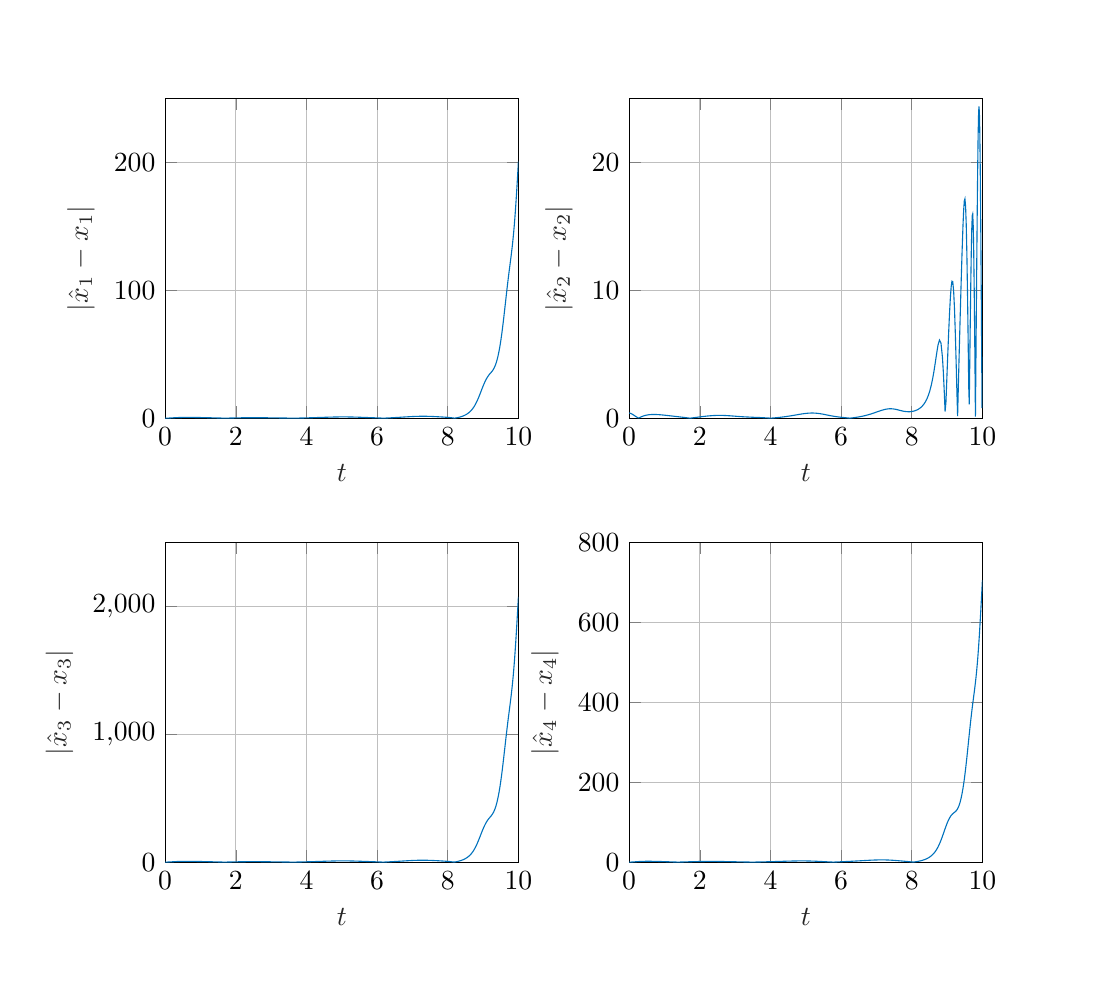
\begin{tikzpicture}

\begin{axis}[%
width=0.37\linewidth,
height=0.335\linewidth,
at={(0\linewidth,0.465\linewidth)},
scale only axis,
xmin=0,
xmax=10,
xlabel style={font=\color{white!15!black}},
xlabel={$t$},
ymin=0,
ymax=250,
ylabel style={font=\color{white!15!black}},
ylabel={$|\hat x_1 - x_1|$},
axis background/.style={fill=white},
xmajorgrids,
ymajorgrids
]
\addplot [color=mycolor1, forget plot]
  table[row sep=crcr]{%
0	0.002\\
0.000178417029156271	0.00205841828298114\\
0.000356834058312542	0.00211593036615143\\
0.000535251087468813	0.0021725378303149\\
0.000713668116625084	0.00222824225445573\\
0.00160575326240644	0.00249327391374332\\
0.0024978384081878	0.00273596537434628\\
0.00338992355396915	0.00295651196812596\\
0.00428200869975051	0.00315510790389117\\
0.00874243442865728	0.0038255523805143\\
0.0132028601575641	0.00397571835766952\\
0.0176632858864708	0.00362863795315405\\
0.0221237116153776	0.00280668643529813\\
0.0379624479282651	0.00362709161087593\\
0.0538011842411526	0.0148758790828974\\
0.0696399205540401	0.0301280467775055\\
0.0854786568669277	0.0486511816569007\\
0.104518190123929	0.074327861011544\\
0.123557723380931	0.102818558242602\\
0.142597256637933	0.133281875749841\\
0.161636789894934	0.164982284522758\\
0.184754110311784	0.204236158057569\\
0.207871430728634	0.243513455998987\\
0.230988751145485	0.282101990976695\\
0.254106071562335	0.319407409723463\\
0.280545594271983	0.359909291522282\\
0.306985116981632	0.397697426372827\\
0.33342463969128	0.432469984745949\\
0.359864162400929	0.463997934766446\\
0.389966777126792	0.495781471631933\\
0.420069391852654	0.52323015688626\\
0.450172006578517	0.54644706080632\\
0.48027462130438	0.565545509939379\\
0.514678811154934	0.582540967627339\\
0.549083001005487	0.594781613038079\\
0.583487190856041	0.602671892516673\\
0.617891380706595	0.606566247860493\\
0.663023553466504	0.606196947330962\\
0.708155726226414	0.600483947415793\\
0.753287898986323	0.590255218822527\\
0.798420071746233	0.576147612596331\\
0.859301430150392	0.551971778370964\\
0.920182788554552	0.523212299481034\\
0.981064146958711	0.490962952838693\\
1.04194550536287	0.455939295164233\\
1.09747200573599	0.422084243638536\\
1.1529985061091	0.38680508622317\\
1.20852500648222	0.350317227445736\\
1.26405150685533	0.312859187032577\\
1.32673314109095	0.269698224108039\\
1.38941477532657	0.225615986671108\\
1.45209640956219	0.180676979496\\
1.51477804379781	0.135175212608206\\
1.58476498039001	0.0841119600175799\\
1.65475191698221	0.0328987166851339\\
1.72473885357441	0.0181023644174846\\
1.79472579016661	0.068217260159339\\
1.88480308448625	0.130284897737669\\
1.97488037880589	0.188290204460219\\
2.06495767312553	0.240519123672296\\
2.15503496744517	0.285203372109176\\
2.25693032557634	0.324338526943179\\
2.35882568370751	0.350307762221941\\
2.46072104183868	0.362773563153615\\
2.56261639996985	0.361431151543136\\
2.64825924393788	0.349673397297776\\
2.73390208790591	0.33118423841879\\
2.81954493187395	0.308530103201917\\
2.90518777584198	0.28216988243004\\
2.9817967362064	0.256072256246507\\
3.05840569657082	0.229263256177172\\
3.13501465693524	0.20211392647229\\
3.21162361729966	0.174809143532548\\
3.29545204705276	0.145520835860014\\
3.37928047680587	0.114763733366214\\
3.46310890655897	0.0805720094878095\\
3.54693733631208	0.0439289964117231\\
3.62177085401317	0.00992217896824155\\
3.69660437171426	0.0275733704326315\\
3.77143788941536	0.0693870388007033\\
3.84627140711645	0.115085820506646\\
3.93186166883489	0.17137726294298\\
4.01745193055334	0.233375000486427\\
4.10304219227178	0.301365097397917\\
4.18863245399022	0.373914736561916\\
4.27722667424324	0.452172146331097\\
4.36582089449626	0.533499137352234\\
4.45441511474929	0.616321254600161\\
4.54300933500231	0.697789145682203\\
4.63637531273009	0.778720945279869\\
4.72974129045787	0.851222438447019\\
4.82310726818565	0.910995620740006\\
4.91647324591343	0.953378009242615\\
4.9867668823177	0.971082853035584\\
5.05706051872197	0.975694648136351\\
5.12735415512623	0.966826315616767\\
5.1976477915305	0.944085534639173\\
5.26794142793477	0.90736230726558\\
5.33823506433903	0.859369513356211\\
5.4085287007433	0.802887187236611\\
5.47882233714757	0.739284656429665\\
5.54353212614873	0.675850627005622\\
5.60824191514989	0.610370768945137\\
5.67295170415105	0.544256998138347\\
5.73766149315221	0.478087233181736\\
5.79544944089558	0.419341705021528\\
5.85323738863896	0.36060862862769\\
5.91102533638233	0.301186831225358\\
5.9688132841257	0.240956904431424\\
6.02660123186907	0.179834566052832\\
6.08438917961245	0.116400955445529\\
6.14217712735582	0.0496677476224732\\
6.19996507509919	0.0204245453650567\\
6.25899708510857	0.0954396476846741\\
6.31802909511794	0.174880771518647\\
6.37706110512732	0.259099817874604\\
6.4360931151367	0.347726288525457\\
6.4959639126223	0.441576917828517\\
6.55583471010791	0.539337634088881\\
6.61570550759352	0.640382582503265\\
6.67557630507913	0.743584293589525\\
6.75036650325845	0.873409506608522\\
6.82515670143776	1.0016367892501\\
6.89994689961708	1.12453053827601\\
6.9747370977964	1.23731161092309\\
7.06501876282321	1.35202143935052\\
7.15530042785002	1.43639580550019\\
7.24558209287683	1.48407835455307\\
7.33586375790364	1.48854756524487\\
7.39427829276798	1.4667903420726\\
7.45269282763233	1.42854921952606\\
7.51110736249667	1.3763254867323\\
7.56952189736102	1.31198086534513\\
7.62793643222536	1.23770553531419\\
7.68635096708971	1.15663413747551\\
7.74476550195406	1.07035816867506\\
7.8031800368184	0.97885947171566\\
7.85180853748465	0.898403203132762\\
7.9004370381509	0.812117962770288\\
7.94906553881715	0.717164791599449\\
7.99769403948341	0.611488662770994\\
8.04632254014966	0.492901452316856\\
8.09495104081591	0.355516933304419\\
8.14357954148216	0.193309232899328\\
8.19220804214841	0.00157029070334769\\
8.23982768556392	0.219960010858642\\
8.28744732897943	0.485061235296969\\
8.33506697239495	0.804894494075766\\
8.38268661581046	1.19074353117412\\
8.42538992081576	1.60434108452431\\
8.46809322582106	2.09809629555675\\
8.51079653082637	2.69089658227603\\
8.55349983583167	3.4048322852587\\
8.59010254804154	4.13444347738644\\
8.62670526025141	4.99479423348042\\
8.66330797246128	6.01021976490817\\
8.69991068467115	7.21104498494914\\
8.74198281523799	8.8642486130529\\
8.78405494580482	10.8442761249588\\
8.82612707637166	13.1623766313575\\
8.86819920693849	15.803356664802\\
8.89325396451413	17.507243984322\\
8.91830872208976	19.2730523492695\\
8.9433634796654	21.0677478451591\\
8.96841823724103	22.8581914594733\\
8.99347299481667	24.610702192904\\
9.0185277523923	26.2925754086391\\
9.04358250996794	27.8769525593491\\
9.06863726754357	29.3435014243276\\
9.09150541010144	30.5677082630884\\
9.1143735526593	31.6759044361815\\
9.13724169521716	32.6685268541551\\
9.16010983777503	33.5550882266341\\
9.18454580457801	34.4072365937323\\
9.20898177138098	35.1966418822482\\
9.23341773818396	35.9729911664474\\
9.25785370498694	36.8003407327165\\
9.27786902154505	37.5658215076229\\
9.29788433810317	38.450980216633\\
9.31789965466128	39.4919903862926\\
9.33791497121939	40.7198459522884\\
9.36592131740018	42.8067358543231\\
9.39392766358096	45.3760243603968\\
9.42193400976174	48.4756037232477\\
9.44994035594253	52.1542364124321\\
9.46840810140955	54.9163427963517\\
9.48687584687657	57.9532058883589\\
9.5053435923436	61.267729245618\\
9.52381133781062	64.8555317322595\\
9.54227908327764	68.7030749964039\\
9.56074682874467	72.7866382116734\\
9.57921457421169	77.0710179031832\\
9.59768231967871	81.507563786059\\
9.61281558675494	85.2169632482787\\
9.62794885383117	88.9602335276555\\
9.64308212090741	92.7071606144901\\
9.65821538798364	96.4299039315315\\
9.67172151679969	99.7119291068454\\
9.68522764561573	102.939913995077\\
9.69873377443178	106.102570776667\\
9.71223990324783	109.194034206644\\
9.72596837154835	112.264124151363\\
9.73969683984887	115.267882831847\\
9.7534253081494	118.221222125827\\
9.76715377644992	121.15203810805\\
9.7788444151093	123.657187357852\\
9.79053505376869	126.197555345461\\
9.80222569242807	128.800828124079\\
9.81391633108746	131.49516377457\\
9.82640226791932	134.505154836563\\
9.83888820475118	137.684459316922\\
9.85137414158304	141.063799540212\\
9.86386007841491	144.670570019504\\
9.87634601524677	148.527715056088\\
9.88883195207863	152.655403679473\\
9.90131788891049	157.067101841024\\
9.91380382574235	161.766582431528\\
9.92479235693768	166.136574404414\\
9.935780888133	170.716633919318\\
9.94676941932833	175.491885091486\\
9.95775795052366	180.441477963236\\
9.96831846289274	185.33936153189\\
9.97887897526183	190.35170341542\\
9.98943948763091	195.454168283693\\
10	200.622751202061\\
};
\end{axis}

\begin{axis}[%
width=0.37\linewidth,
height=0.335\linewidth,
at={(0.486\linewidth,0.465\linewidth)},
scale only axis,
xmin=0,
xmax=10,
xlabel style={font=\color{white!15!black}},
xlabel={$t$},
ymin=0,
ymax=25,
ylabel style={font=\color{white!15!black}},
ylabel={$|\hat x_2 - x_2|$},
axis background/.style={fill=white},
xmajorgrids,
ymajorgrids
]
\addplot [color=mycolor1, forget plot]
  table[row sep=crcr]{%
0	0.402\\
0.000178417029156271	0.401937966016663\\
0.000356834058312542	0.401875197663619\\
0.000535251087468813	0.401811696358309\\
0.000713668116625084	0.401747463516458\\
0.00160575326240644	0.401415375691345\\
0.0024978384081878	0.401065210826695\\
0.00338992355396915	0.400697143965451\\
0.00428200869975051	0.400311349092612\\
0.00874243442865728	0.398122475795928\\
0.0132028601575641	0.395515893386791\\
0.0176632858864708	0.392512176234593\\
0.0221237116153776	0.389131279201939\\
0.0379624479282651	0.374364852035779\\
0.0538011842411526	0.355882323083196\\
0.0696399205540401	0.334397021110357\\
0.0854786568669277	0.310547835710007\\
0.104518190123929	0.27954389047824\\
0.123557723380931	0.246762286611258\\
0.142597256637933	0.212907582394928\\
0.161636789894934	0.178587098564349\\
0.184754110311784	0.13701746530933\\
0.207871430728634	0.0961930138664254\\
0.230988751145485	0.0566525109966843\\
0.254106071562335	0.0188343888996587\\
0.280545594271983	0.0218912865323947\\
0.306985116981632	0.0596783283841005\\
0.33342463969128	0.0943682634460381\\
0.359864162400929	0.125852994793299\\
0.389966777126792	0.157758883258937\\
0.420069391852654	0.185609154373787\\
0.450172006578517	0.209582978154567\\
0.48027462130438	0.229851223977686\\
0.514678811154934	0.248737444674336\\
0.549083001005487	0.263478010245589\\
0.583487190856041	0.274483098004209\\
0.617891380706595	0.282107200784661\\
0.663023553466504	0.287551050841689\\
0.708155726226414	0.288640350120763\\
0.753287898986323	0.286147425923358\\
0.798420071746233	0.28067652138211\\
0.859301430150392	0.269540670933609\\
0.920182788554552	0.255286103939565\\
0.981064146958711	0.238904518771727\\
1.04194550536287	0.221098244158487\\
1.09747200573599	0.204107148064304\\
1.1529985061091	0.186707360875311\\
1.20852500648222	0.169047462083928\\
1.26405150685533	0.151296189922408\\
1.32673314109095	0.131320645598063\\
1.38941477532657	0.111249790464363\\
1.45209640956219	0.0909451143263133\\
1.51477804379781	0.0704562246988213\\
1.58476498039001	0.0474131925002125\\
1.65475191698221	0.0238974859240998\\
1.72473885357441	0.000200670682820592\\
1.79472579016661	0.0247295667453244\\
1.88480308448625	0.0566628682643106\\
1.97488037880589	0.0886551095865502\\
2.06495767312553	0.119851376224218\\
2.15503496744517	0.149079801120144\\
2.25693032557634	0.177804383086948\\
2.35882568370751	0.200212160188533\\
2.46072104183868	0.214769510854481\\
2.56261639996985	0.219755310525512\\
2.64825924393788	0.215495135363167\\
2.73390208790591	0.20544202258621\\
2.81954493187395	0.19158121702854\\
2.90518777584198	0.174504049752252\\
2.9817967362064	0.157477227521746\\
3.05840569657082	0.140649279463768\\
3.13501465693524	0.124765370896985\\
3.21162361729966	0.11045821802937\\
3.29545204705276	0.0978363299178884\\
3.37928047680587	0.0866194713593158\\
3.46310890655897	0.0751570206735501\\
3.54693733631208	0.0646708642894308\\
3.62177085401317	0.0569754336744354\\
3.69660437171426	0.0486287377811593\\
3.77143788941536	0.0388396622362098\\
3.84627140711645	0.0279652628369075\\
3.93186166883489	0.0146977058412663\\
4.01745193055334	0.001169860219351\\
4.10304219227178	0.0204454356596799\\
4.18863245399022	0.0425095764779776\\
4.27722667424324	0.0678816541833594\\
4.36582089449626	0.0972104265702091\\
4.45441511474929	0.130751849883272\\
4.54300933500231	0.167883560879803\\
4.63637531273009	0.210106243379477\\
4.72974129045787	0.254728251485407\\
4.82310726818565	0.299455016417752\\
4.91647324591343	0.340730813098622\\
4.9867668823177	0.366830125247433\\
5.05706051872197	0.386852440443225\\
5.12735415512623	0.399187415137422\\
5.1976477915305	0.402040722345297\\
5.26794142793477	0.393826837606004\\
5.33823506433903	0.375671603641962\\
5.4085287007433	0.349296126802834\\
5.47882233714757	0.315870006953751\\
5.54353212614873	0.280581666262108\\
5.60824191514989	0.243962470533536\\
5.67295170415105	0.208054077909433\\
5.73766149315221	0.174265475247654\\
5.79544944089558	0.146927851038236\\
5.85323738863896	0.122299363717728\\
5.91102533638233	0.0999792258566069\\
5.9688132841257	0.080062002220474\\
6.02660123186907	0.0625580745792441\\
6.08438917961245	0.0460664734611814\\
6.14217712735582	0.0295690018948832\\
6.19996507509919	0.0128911308811158\\
6.25899708510857	0.00450070946393843\\
6.31802909511794	0.0234834467435345\\
6.37706110512732	0.0447728404946713\\
6.4360931151367	0.068532460374694\\
6.4959639126223	0.0953310531775246\\
6.55583471010791	0.125608559160119\\
6.61570550759352	0.159785984773326\\
6.67557630507913	0.198021532243831\\
6.75036650325845	0.251620790126672\\
6.82515670143776	0.312074103228244\\
6.89994689961708	0.378793805167216\\
6.9747370977964	0.44996927481891\\
7.06501876282321	0.53725599996977\\
7.15530042785002	0.619707784297655\\
7.24558209287683	0.688139924991331\\
7.33586375790364	0.729898471586255\\
7.39427829276798	0.737141920395114\\
7.45269282763233	0.729360335961701\\
7.51110736249667	0.708092101071264\\
7.56952189736102	0.675553518379204\\
7.62793643222536	0.63568049075945\\
7.68635096708971	0.594170102288955\\
7.74476550195406	0.556006663654307\\
7.8031800368184	0.52566488064083\\
7.85180853748465	0.509756432513132\\
7.9004370381509	0.502913245332863\\
7.94906553881715	0.505227772381849\\
7.99769403948341	0.518621081373528\\
8.04632254014966	0.545642254844554\\
8.09495104081591	0.584949588576317\\
8.14357954148216	0.637099103751462\\
8.19220804214841	0.706779718590482\\
8.23982768556392	0.798382865041191\\
8.28744732897943	0.915388642546225\\
8.33506697239495	1.0642315271687\\
8.38268661581046	1.25808846191029\\
8.42538992081576	1.48421921061648\\
8.46809322582106	1.77083755698276\\
8.51079653082637	2.13253202572068\\
8.55349983583167	2.58898396192552\\
8.59010254804154	3.06820547123606\\
8.62670526025141	3.63782031944356\\
8.66330797246128	4.28702949809354\\
8.69991068467115	4.97246278253884\\
8.74198281523799	5.69899467782872\\
8.78405494580482	6.10212705543648\\
8.82612707637166	5.88497431951694\\
8.86819920693849	4.77694124052915\\
8.89325396451413	3.63246190421212\\
8.91830872208976	2.18780309017495\\
8.9433634796654	0.517184574790845\\
8.96841823724103	1.28407745913632\\
8.99347299481667	3.11989466057088\\
9.0185277523923	4.92496410996662\\
9.04358250996794	6.63143743504959\\
9.06863726754357	8.16761555437086\\
9.09150541010144	9.35367660917532\\
9.1143735526593	10.2352747001096\\
9.13724169521716	10.706701307348\\
9.16010983777503	10.6676672147608\\
9.18454580457801	9.97805920223039\\
9.20898177138098	8.60602456439824\\
9.23341773818396	6.62519227556042\\
9.25785370498694	4.20863631118842\\
9.27786902154505	2.05458697771311\\
9.29788433810317	0.168974797530019\\
9.31789965466128	2.39141562484686\\
9.33791497121939	4.56424228168603\\
9.36592131740018	7.46482526292495\\
9.39392766358096	10.2187286995163\\
9.42193400976174	12.7916573367331\\
9.44994035594253	15.0363434725715\\
9.46840810140955	16.2109227705996\\
9.48687584687657	16.9714312583634\\
9.5053435923436	17.1433899836254\\
9.52381133781062	16.5623108304526\\
9.54227908327764	15.110953077626\\
9.56074682874467	12.7571205468455\\
9.57921457421169	9.57690130248039\\
9.59768231967871	5.78707172716006\\
9.61281558675494	2.41587703163839\\
9.62794885383117	1.08424738858631\\
9.64308212090741	4.58359388866135\\
9.65821538798364	7.93728342628829\\
9.67172151679969	10.6781349800245\\
9.68522764561573	13.0231279878747\\
9.69873377443178	14.7993283912863\\
9.71223990324783	15.8318855655629\\
9.72596837154835	15.9610678063736\\
9.73969683984887	15.0551519580908\\
9.7534253081494	13.1064917685369\\
9.76715377644992	10.236640623846\\
9.7788444151093	7.21908345885487\\
9.79053505376869	3.8028337229825\\
9.80222569242807	0.118580265919984\\
9.81391633108746	3.70529089457853\\
9.82640226791932	7.81348417600386\\
9.83888820475118	11.8240730365563\\
9.85137414158304	15.588710463655\\
9.86386007841491	18.9353555251622\\
9.87634601524677	21.6737618269552\\
9.88883195207863	23.5541271680831\\
9.90131788891049	24.3594216843456\\
9.91380382574235	23.9554358020063\\
9.92479235693768	22.566608607994\\
9.935780888133	20.2560428424254\\
9.94676941932833	17.1337269368227\\
9.95775795052366	13.3797234344924\\
9.96831846289274	9.36744969713622\\
9.97887897526183	5.11311771118979\\
9.98943948763091	0.792925704654769\\
10	3.39976802900753\\
};
\end{axis}

\begin{axis}[%
width=0.37\linewidth,
height=0.335\linewidth,
at={(0\linewidth,0\linewidth)},
scale only axis,
xmin=0,
xmax=10,
xlabel style={font=\color{white!15!black}},
xlabel={$t$},
ymin=0,
ymax=2500,
ylabel style={font=\color{white!15!black}},
ylabel={$|\hat x_3 - x_3|$},
axis background/.style={fill=white},
xmajorgrids,
ymajorgrids
]
\addplot [color=mycolor1, forget plot]
  table[row sep=crcr]{%
0	0.01\\
0.000178417029156271	0.00988706071311102\\
0.000356834058312542	0.00976639211968588\\
0.000535251087468813	0.00963800841321424\\
0.000713668116625084	0.00950192377041001\\
0.00160575326240644	0.00870648153991795\\
0.0024978384081878	0.00772063276975468\\
0.00338992355396915	0.00654613073752791\\
0.00428200869975051	0.00518471837355892\\
0.00874243442865728	0.0043656634265639\\
0.0132028601575641	0.0183332911864801\\
0.0176632858864708	0.0365117554947688\\
0.0221237116153776	0.0587006868745943\\
0.0379624479282651	0.16701636974496\\
0.0538011842411526	0.315425671382345\\
0.0696399205540401	0.49670423660663\\
0.0854786568669277	0.704349141747662\\
0.104518190123929	0.980721799774114\\
0.123557723380931	1.27832079584864\\
0.142597256637933	1.58977772903158\\
0.161636789894934	1.908675254863\\
0.184754110311784	2.29807820653404\\
0.207871430728634	2.68293048869602\\
0.230988751145485	3.05719118840285\\
0.254106071562335	3.4158546294019\\
0.280545594271983	3.80203537941032\\
0.306985116981632	4.15940565387458\\
0.33342463969128	4.48569148079881\\
0.359864162400929	4.77922914427867\\
0.389966777126792	5.07256835068624\\
0.420069391852654	5.32327190679639\\
0.450172006578517	5.53271531431228\\
0.48027462130438	5.70231299248618\\
0.514678811154934	5.84970358971852\\
0.549083001005487	5.95159771646049\\
0.583487190856041	6.01204096868095\\
0.617891380706595	6.03457692378225\\
0.663023553466504	6.01240580938522\\
0.708155726226414	5.93988805091989\\
0.753287898986323	5.82493073651747\\
0.798420071746233	5.6736556770477\\
0.859301430150392	5.42163638252704\\
0.920182788554552	5.12682981511188\\
0.981064146958711	4.79936350206454\\
1.04194550536287	4.44599954934458\\
1.09747200573599	4.10588596639879\\
1.1529985061091	3.7523251285645\\
1.20852500648222	3.38726958641686\\
1.26405150685533	3.01293577428521\\
1.32673314109095	2.58191528224147\\
1.38941477532657	2.14205421348026\\
1.45209640956219	1.69408563444539\\
1.51477804379781	1.24091457756778\\
1.58476498039001	0.732814617502389\\
1.65475191698221	0.224093852201825\\
1.72473885357441	0.281331568506748\\
1.79472579016661	0.776668909723421\\
1.88480308448625	1.3879925786234\\
1.97488037880589	1.95605845687618\\
2.06495767312553	2.46362034014932\\
2.15503496744517	2.89346154005469\\
2.25693032557634	3.26389667956972\\
2.35882568370751	3.5016585710917\\
2.46072104183868	3.60475334263371\\
2.56261639996985	3.57244078251582\\
2.64825924393788	3.44310528894913\\
2.73390208790591	3.24971059791379\\
2.81954493187395	3.01730360135468\\
2.90518777584198	2.75113304597719\\
2.9817967362064	2.49065782516623\\
3.05840569657082	2.22415384975698\\
3.13501465693524	1.95456800141403\\
3.21162361729966	1.68316285739159\\
3.29545204705276	1.39034255880844\\
3.37928047680587	1.08172098455128\\
3.46310890655897	0.738558808852865\\
3.54693733631208	0.369361935294513\\
3.62177085401317	0.0243701072120928\\
3.69660437171426	0.356129858105902\\
3.77143788941536	0.779642841349123\\
3.84627140711645	1.24226899341664\\
3.93186166883489	1.81263700558934\\
4.01745193055334	2.43932815485515\\
4.10304219227178	3.12414649014401\\
4.18863245399022	3.85314731423216\\
4.27722667424324	4.63819595876252\\
4.36582089449626	5.45080044690048\\
4.45441511474929	6.2740298600552\\
4.54300933500231	7.07919609071002\\
4.63637531273009	7.87346228221273\\
4.72974129045787	8.57654661781368\\
4.82310726818565	9.14511436256019\\
4.91647324591343	9.53412066342288\\
4.9867668823177	9.68275069728024\\
5.05706051872197	9.6992589646503\\
5.12735415512623	9.58104242813938\\
5.1976477915305	9.3261693757474\\
5.26794142793477	8.9358950162434\\
5.33823506433903	8.4377771553947\\
5.4085287007433	7.85979952093572\\
5.47882233714757	7.2165565741899\\
5.54353212614873	6.58102015869198\\
5.60824191514989	5.92837595935298\\
5.67295170415105	5.27130513971967\\
5.73766149315221	4.61462606282017\\
5.79544944089558	4.03139401956471\\
5.85323738863896	3.4473072835087\\
5.91102533638233	2.85512174683451\\
5.9688132841257	2.2530436459758\\
6.02660123186907	1.6396082662347\\
6.08438917961245	1.00138452825675\\
6.14217712735582	0.329111359918745\\
6.19996507509919	0.377946337250076\\
6.25899708510857	1.13574946312934\\
6.31802909511794	1.93806456252805\\
6.37706110512732	2.78764745351805\\
6.4360931151367	3.68064137617017\\
6.4959639126223	4.62511719837132\\
6.55583471010791	5.60680278478711\\
6.61570550759352	6.61867986771219\\
6.67557630507913	7.64899248692907\\
6.75036650325845	8.94006202889645\\
6.82515670143776	10.2075676325506\\
6.89994689961708	11.4126355512149\\
6.9747370977964	12.5071678189452\\
7.06501876282321	13.6028294986658\\
7.15530042785002	14.3819914102099\\
7.24558209287683	14.7841838240176\\
7.33586375790364	14.754387192022\\
7.39427829276798	14.4945599608244\\
7.45269282763233	14.0758567789987\\
7.51110736249667	13.5244259330863\\
7.56952189736102	12.859794588669\\
7.62793643222536	12.1038546950888\\
7.68635096708971	11.284758091856\\
7.74476550195406	10.4148473077141\\
7.8031800368184	9.49098669624523\\
7.85180853748465	8.67471766607854\\
7.9004370381509	7.7937303187755\\
7.94906553881715	6.81802294950099\\
7.99769403948341	5.7244958528878\\
8.04632254014966	4.4878943834652\\
8.09495104081591	3.04855567361843\\
8.14357954148216	1.34462765802417\\
8.19220804214841	0.675497097095331\\
8.23982768556392	3.01778474011168\\
8.28744732897943	5.82541031334792\\
8.33506697239495	9.21623410202974\\
8.38268661581046	13.3142549049617\\
8.42538992081576	17.7170676052081\\
8.46809322582106	22.9823542936378\\
8.51079653082637	29.3140010853348\\
8.55349983583167	36.952173514145\\
8.59010254804154	44.7665014866288\\
8.62670526025141	53.991662776649\\
8.66330797246128	64.8852828003392\\
8.69991068467115	77.7508779641788\\
8.74198281523799	95.3941652803255\\
8.78405494580482	116.372702545619\\
8.82612707637166	140.662248969076\\
8.86819920693849	167.905474117142\\
8.89325396451413	185.212339615179\\
8.91830872208976	202.931014471598\\
8.9433634796654	220.719299956302\\
8.96841823724103	238.251277807579\\
8.99347299481667	255.214098119837\\
9.0185277523923	271.313787447906\\
9.04358250996794	286.319336823983\\
9.06863726754357	300.07224961626\\
9.09150541010144	311.45901210496\\
9.1143735526593	321.711392274282\\
9.13724169521716	330.891557669572\\
9.16010983777503	339.163116514977\\
9.18454580457801	347.301424208589\\
9.20898177138098	355.162150568417\\
9.23341773818396	363.308013555268\\
9.25785370498694	372.406114573949\\
9.27786902154505	381.059283649383\\
9.29788433810317	391.173991993302\\
9.31789965466128	403.081054323455\\
9.33791497121939	417.059226345248\\
9.36592131740018	440.579413756207\\
9.39392766358096	469.189217077333\\
9.42193400976174	503.316361097078\\
9.44994035594253	543.381595155841\\
9.46840810140955	573.204675176396\\
9.48687584687657	605.758924186156\\
9.5053435923436	641.008992382891\\
9.52381133781062	678.827616575866\\
9.54227908327764	718.985392513128\\
9.56074682874467	761.144705975121\\
9.57921457421169	804.875917627194\\
9.59768231967871	849.654553266528\\
9.61281558675494	886.735160145913\\
9.62794885383117	923.854413881586\\
9.64308212090741	960.739253727003\\
9.65821538798364	997.157629789586\\
9.67172151679969	1029.11496068437\\
9.68522764561573	1060.45197533361\\
9.69873377443178	1091.12188359447\\
9.71223990324783	1121.14701606225\\
9.72596837154835	1151.10610773199\\
9.73969683984887	1180.67156053465\\
9.7534253081494	1210.10012803027\\
9.76715377644992	1239.74716477489\\
9.7788444151093	1265.47632339578\\
9.79053505376869	1291.9309537039\\
9.80222569242807	1319.38805821373\\
9.81391633108746	1348.11501571735\\
9.82640226791932	1380.48638288707\\
9.83888820475118	1414.89250697961\\
9.85137414158304	1451.5914736075\\
9.86386007841491	1490.79362678838\\
9.87634601524677	1532.65323318685\\
9.88883195207863	1577.27876329332\\
9.90131788891049	1624.697213583\\
9.91380382574235	1674.83045108437\\
9.92479235693768	1721.06564637013\\
9.935780888133	1769.11449580232\\
9.94676941932833	1818.77268335949\\
9.95775795052366	1869.79917024629\\
9.96831846289274	1919.88624246742\\
9.97887897526183	1970.76609850055\\
9.98943948763091	2022.21491287598\\
10	2074.03156986629\\
};
\end{axis}

\begin{axis}[%
width=0.37\linewidth,
height=0.335\linewidth,
at={(0.486\linewidth,0\linewidth)},
scale only axis,
xmin=0,
xmax=10,
xlabel style={font=\color{white!15!black}},
xlabel={$t$},
ymin=0,
ymax=800,
ylabel style={font=\color{white!15!black}},
ylabel={$|\hat x_4 - x_4|$},
axis background/.style={fill=white},
xmajorgrids,
ymajorgrids
]
\addplot [color=mycolor1, forget plot]
  table[row sep=crcr]{%
0	0.01\\
0.000178417029156271	0.009952209789599\\
0.000356834058312542	0.00990121620439163\\
0.000535251087468813	0.00984702542921308\\
0.000713668116625084	0.00978964364136863\\
0.00160575326240644	0.00945508519900717\\
0.0024978384081878	0.0090416737096162\\
0.00338992355396915	0.00855017289347398\\
0.00428200869975051	0.0079813418283384\\
0.00874243442865728	0.00400350182376485\\
0.0132028601575641	0.00179639183032682\\
0.0176632858864708	0.00932859240486061\\
0.0221237116153776	0.018506057097719\\
0.0379624479282651	0.0631380607060368\\
0.0538011842411526	0.123978517103876\\
0.0696399205540401	0.197911363273616\\
0.0854786568669277	0.282140142603811\\
0.104518190123929	0.39353538603675\\
0.123557723380931	0.51260880823268\\
0.142597256637933	0.636245875271506\\
0.161636789894934	0.761747506378341\\
0.184754110311784	0.913381952336633\\
0.207871430728634	1.06134358365948\\
0.230988751145485	1.20319055585826\\
0.254106071562335	1.33692229667872\\
0.280545594271983	1.47801212639592\\
0.306985116981632	1.60531824798248\\
0.33342463969128	1.71809818269939\\
0.359864162400929	1.81585364717301\\
0.389966777126792	1.90869518925364\\
0.420069391852654	1.98255181952555\\
0.450172006578517	2.03829046293479\\
0.48027462130438	2.07676403618913\\
0.514678811154934	2.10088920064312\\
0.549083001005487	2.10587743835057\\
0.583487190856041	2.09373569357793\\
0.617891380706595	2.06621669043942\\
0.663023553466504	2.00960015882278\\
0.708155726226414	1.93363508979074\\
0.753287898986323	1.84201718269809\\
0.798420071746233	1.73761307831819\\
0.859301430150392	1.5809673288511\\
0.920182788554552	1.41167678618685\\
0.981064146958711	1.23425268802645\\
1.04194550536287	1.05173287295013\\
1.09747200573599	0.882923913805783\\
1.1529985061091	0.713370933498043\\
1.20852500648222	0.543872916627238\\
1.26405150685533	0.375355701603598\\
1.32673314109095	0.187411094439421\\
1.38941477532657	0.00182557908536207\\
1.45209640956219	0.181207525801238\\
1.51477804379781	0.360555613541257\\
1.58476498039001	0.554907461751826\\
1.65475191698221	0.742624933082306\\
1.72473885357441	0.922363619257244\\
1.79472579016661	1.09162494098479\\
1.88480308448625	1.29004831808321\\
1.97488037880589	1.46189915579378\\
2.06495767312553	1.60133006048094\\
2.15503496744517	1.70288189579289\\
2.25693032557634	1.76514973316889\\
2.35882568370751	1.77063463707319\\
2.46072104183868	1.72172252627708\\
2.56261639996985	1.62060853722636\\
2.64825924393788	1.49779100980673\\
2.73390208790591	1.35432130911918\\
2.81954493187395	1.20166347105541\\
2.90518777584198	1.04199705841373\\
2.9817967362064	0.895732916427136\\
3.05840569657082	0.752662346783051\\
3.13501465693524	0.613785190096792\\
3.21162361729966	0.479531982839141\\
3.29545204705276	0.340617665512241\\
3.37928047680587	0.20110993029461\\
3.46310890655897	0.0529505621869149\\
3.54693733631208	0.0996381640140473\\
3.62177085401317	0.236301263538072\\
3.69660437171426	0.382261248906943\\
3.77143788941536	0.540340281492986\\
3.84627140711645	0.708399329441702\\
3.93186166883489	0.909419324094626\\
4.01745193055334	1.12463438272042\\
4.10304219227178	1.35432640567796\\
4.18863245399022	1.59208522081654\\
4.27722667424324	1.83961733695531\\
4.36582089449626	2.08724524755996\\
4.45441511474929	2.3281334678003\\
4.54300933500231	2.55092968166649\\
4.63637531273009	2.75298310232767\\
4.72974129045787	2.90851561853925\\
4.82310726818565	3.00203530887516\\
4.91647324591343	3.01830975066001\\
4.9867668823177	2.97131569950883\\
5.05706051872197	2.87215712683603\\
5.12735415512623	2.72175739749256\\
5.1976477915305	2.52102171390277\\
5.26794142793477	2.27193381837274\\
5.33823506433903	1.98780561060234\\
5.4085287007433	1.68161621614745\\
5.47882233714757	1.35980517237842\\
5.54353212614873	1.05579334207541\\
5.60824191514989	0.754764826361068\\
5.67295170415105	0.461802264150087\\
5.73766149315221	0.178619360322795\\
5.79544944089558	0.0650294437355718\\
5.85323738863896	0.301900912841788\\
5.91102533638233	0.5352724311823\\
5.9688132841257	0.765873978589328\\
6.02660123186907	0.994223010195109\\
6.08438917961245	1.22602367713441\\
6.14217712735582	1.46505259316068\\
6.19996507509919	1.71132256293814\\
6.25899708510857	1.96987647159632\\
6.31802909511794	2.23888364676657\\
6.37706110512732	2.51920013096796\\
6.4360931151367	2.8088792399028\\
6.4959639126223	3.10963418757675\\
6.55583471010791	3.41645223901127\\
6.61570550759352	3.72629182582153\\
6.67557630507913	4.034252561901\\
6.75036650325845	4.40749573941649\\
6.82515670143776	4.75697011659605\\
6.89994689961708	5.06770131962997\\
6.9747370977964	5.32162767690135\\
7.06501876282321	5.52357215322809\\
7.15530042785002	5.58794321817705\\
7.24558209287683	5.49664888451576\\
7.33586375790364	5.23424754145211\\
7.39427829276798	4.97254301037961\\
7.45269282763233	4.65369217624538\\
7.51110736249667	4.29031892156582\\
7.56952189736102	3.89150264655852\\
7.62793643222536	3.46707349869188\\
7.68635096708971	3.02938597533681\\
7.74476550195406	2.58384774639415\\
7.8031800368184	2.12946662383613\\
7.85180853748465	1.74232329601608\\
7.9004370381509	1.3381804107432\\
7.94906553881715	0.904961398380038\\
7.99769403948341	0.434104700092924\\
8.04632254014966	0.083480179935929\\
8.09495104081591	0.671435372552512\\
8.14357954148216	1.35359796814244\\
8.19220804214841	2.14858417324119\\
8.23982768556392	3.05700483401582\\
8.28744732897943	4.13433580122007\\
8.33506697239495	5.42502783815152\\
8.38268661581046	6.97452843839184\\
8.42538992081576	8.63059624572023\\
8.46809322582106	10.604898077362\\
8.51079653082637	12.9743696150354\\
8.55349983583167	15.8288094754121\\
8.59010254804154	18.7468382366274\\
8.62670526025141	22.1906300303691\\
8.66330797246128	26.2562735952473\\
8.69991068467115	31.0569227613833\\
8.74198281523799	37.6385377874984\\
8.78405494580482	45.4478827471746\\
8.82612707637166	54.4476240504897\\
8.86819920693849	64.4669740243558\\
8.89325396451413	70.7777965350723\\
8.91830872208976	77.1773092860455\\
8.9433634796654	83.5227972283485\\
8.96841823724103	89.6810021255192\\
8.99347299481667	95.5257539204315\\
9.0185277523923	100.93958038316\\
9.04358250996794	105.832692035724\\
9.06863726754357	110.146405277918\\
9.09150541010144	113.554365159759\\
9.1143735526593	116.454460952955\\
9.13724169521716	118.87828845997\\
9.16010983777503	120.898866000511\\
9.18454580457801	122.74275074618\\
9.20898177138098	124.44946073586\\
9.23341773818396	126.253206295092\\
9.25785370498694	128.427436907777\\
9.27786902154505	130.683683549391\\
9.29788433810317	133.520358527936\\
9.31789965466128	137.068153185286\\
9.33791497121939	141.434856040248\\
9.36592131740018	149.104160723713\\
9.39392766358096	158.760869212714\\
9.42193400976174	170.551774926571\\
9.44994035594253	184.620687963343\\
9.46840810140955	195.192794481202\\
9.48687584687657	206.792918491169\\
9.5053435923436	219.39673328885\\
9.52381133781062	232.942209828113\\
9.54227908327764	247.325817409993\\
9.56074682874467	262.399802474929\\
9.57921457421169	277.979890852982\\
9.59768231967871	293.844962938737\\
9.61281558675494	306.893534758377\\
9.62794885383117	319.856706777875\\
9.64308212090741	332.622169779655\\
9.65821538798364	345.095588855406\\
9.67172151679969	355.920557966866\\
9.68522764561573	366.413940633479\\
9.69873377443178	376.558666829752\\
9.71223990324783	386.366379154855\\
9.72596837154835	396.034108311291\\
9.73969683984887	405.471031887845\\
9.7534253081494	414.785026794144\\
9.76715377644992	424.123820795812\\
9.7788444151093	432.224250440634\\
9.79053505376869	440.576307570087\\
9.80222569242807	449.293164463099\\
9.81391633108746	458.483210060267\\
9.82640226791932	468.936799713964\\
9.83888820475118	480.165207722491\\
9.85137414158304	492.270262122413\\
9.86386007841491	505.333356790572\\
9.87634601524677	519.412143129819\\
9.88883195207863	534.544923094232\\
9.90131788891049	550.736116691657\\
9.91380382574235	567.946645161886\\
9.92479235693768	583.876802327757\\
9.935780888133	600.467596614845\\
9.94676941932833	617.630672742892\\
9.95775795052366	635.263123819814\\
9.96831846289274	652.548837016176\\
9.97887897526183	670.068882579869\\
9.98943948763091	687.729297396656\\
10	705.446118781245\\
};
\end{axis}

\begin{axis}[%
width=1.104\linewidth,
height=0.982\linewidth,
at={(-0.144\linewidth,-0.108\linewidth)},
scale only axis,
xmin=0,
xmax=1,
ymin=0,
ymax=1,
axis line style={draw=none},
ticks=none,
axis x line*=bottom,
axis y line*=left
]
\end{axis}
\end{tikzpicture}%
	\caption{Абсолютное отклонение оценки от настоящего состояния линейной системы для предыдущей задачи.}
\end{figure}

\begin{figure}[t]
	\centering
	% This file was created by matlab2tikz.
%
%The latest updates can be retrieved from
%  http://www.mathworks.com/matlabcentral/fileexchange/22022-matlab2tikz-matlab2tikz
%where you can also make suggestions and rate matlab2tikz.
%
\definecolor{mycolor1}{rgb}{0.00000,0.44700,0.74100}%
%
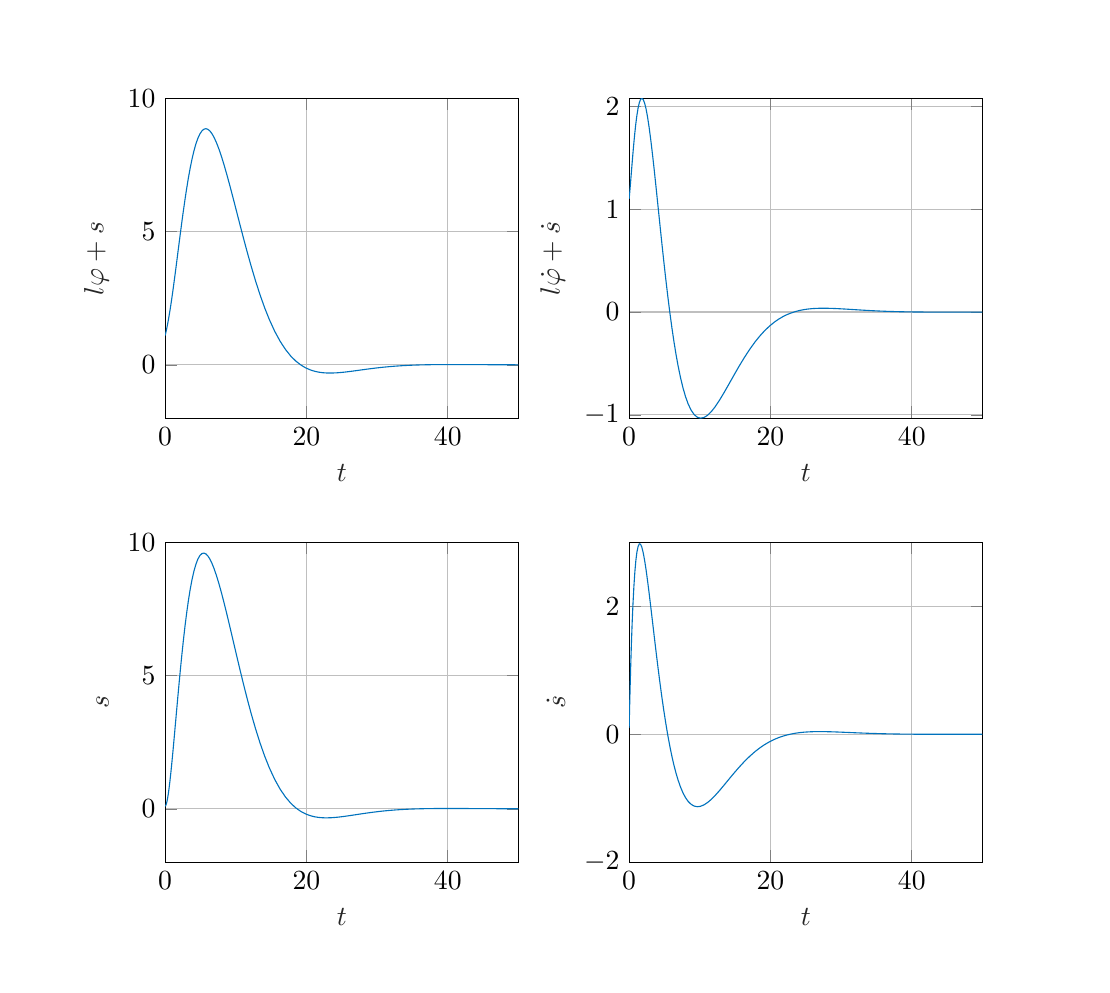
\begin{tikzpicture}

\begin{axis}[%
width=0.37\linewidth,
height=0.335\linewidth,
at={(0\linewidth,0.465\linewidth)},
scale only axis,
xmin=0,
xmax=50,
xlabel style={font=\color{white!15!black}},
xlabel={$t$},
ymin=-2,
ymax=10,
ylabel style={font=\color{white!15!black}},
ylabel={$l\varphi+s$},
axis background/.style={fill=white},
xmajorgrids,
ymajorgrids
]
\addplot [color=mycolor1, forget plot]
  table[row sep=crcr]{%
0	1.1\\
0.000995243685935657	1.10109513961887\\
0.00199048737187131	1.10219102285774\\
0.00298573105780697	1.10328765045123\\
0.00398097474374263	1.10438502313079\\
0.00895719317342091	1.109883088207\\
0.0139334116030992	1.11539988834718\\
0.0189096300327775	1.12093551146464\\
0.0238858484624558	1.12649004355485\\
0.0487669406108472	1.15454923533614\\
0.0736480327592386	1.18309295536601\\
0.09852912490763	1.21212985776172\\
0.123410217056021	1.24166755084622\\
0.225715188625279	1.36853352318656\\
0.328020160194536	1.5042276509553\\
0.430325131763794	1.64877099145836\\
0.532630103333051	1.80205748026874\\
0.672607591253264	2.02548804562654\\
0.812585079173478	2.26346367328115\\
0.952562567093691	2.51438756655666\\
1.0925400550139	2.77667880092482\\
1.26641053186255	3.11573809837491\\
1.44028100871119	3.46566072496721\\
1.61415148555983	3.82256219449829\\
1.78802196240848	4.18304729999551\\
1.98797997906268	4.59785841157988\\
2.18793799571689	5.00793583764913\\
2.3878960123711	5.40878443841498\\
2.58785402902531	5.79673892197609\\
2.82486349339164	6.23553951162071\\
3.06187295775797	6.64694720764001\\
3.2988824221243	7.02726806210098\\
3.53589188649063	7.37388289633296\\
3.8068471260882	7.72646789372818\\
4.07780236568576	8.03080981265043\\
4.34875760528333	8.28628276471194\\
4.6197128448809	8.49304782959164\\
4.90880275471955	8.66090756850989\\
5.1978926645582	8.77631787519747\\
5.48698257439685	8.84183758087253\\
5.7760724842355	8.86022771520226\\
6.06157974672748	8.83513580741115\\
6.34708700921947	8.77051776828554\\
6.63259427171145	8.66982436453451\\
6.91810153420343	8.53639866452068\\
7.27296504620043	8.32991567575342\\
7.62782855819744	8.08458968184668\\
7.98269207019444	7.80668353282753\\
8.33755558219144	7.50187709401966\\
8.76915244007901	7.10255189443271\\
9.20074929796658	6.68055939691282\\
9.63234615585415	6.24411166221094\\
10.0639430137417	5.80019944101074\\
10.5813189291691	5.2667784451128\\
11.0986948445964	4.74071737496048\\
11.6160707600238	4.22951642014299\\
12.1334466754511	3.73901451242217\\
12.7846884065333	3.15797982517782\\
13.4359301376155	2.62309536906756\\
14.0871718686977	2.13797598164852\\
14.7384135997799	1.70445651036672\\
15.5062380404241	1.25995777568309\\
16.2740624810684	0.884379969204405\\
17.0418869217127	0.572982157446099\\
17.809711362357	0.320910952628373\\
18.5012093118346	0.140030750984562\\
19.1927072613122	-0.00259493658587034\\
19.8842052107898	-0.111900865103107\\
20.5757031602675	-0.192305384126489\\
21.1438619700393	-0.239711799909017\\
21.7120207798112	-0.272891944492461\\
22.280179589583	-0.293997990114707\\
22.8483383993549	-0.304954006723109\\
23.4893166646037	-0.30731093870379\\
24.1302949298525	-0.301289640888249\\
24.7712731951013	-0.288900058534427\\
25.4122514603501	-0.271840338118735\\
26.0009145687763	-0.253300719214212\\
26.5895776772026	-0.233009816694561\\
27.1782407856288	-0.211765317552969\\
27.7669038940551	-0.190226863767898\\
28.5427223160121	-0.162290944605133\\
29.3185407379691	-0.135659094499385\\
30.0943591599261	-0.110946542881483\\
30.8701775818831	-0.088579556865304\\
31.6684153389528	-0.0682694477710699\\
32.4666530960225	-0.0507172412378994\\
33.2648908530922	-0.0358406057465539\\
34.063128610162	-0.0235274996629671\\
34.7806300418881	-0.0145040123820123\\
35.4981314736143	-0.00720544291545372\\
36.2156329053405	-0.00143545593288807\\
36.9331343370667	0.00298448015678369\\
37.5458153781539	0.00582320336468613\\
38.1584964192411	0.00792702289106795\\
38.7711774603283	0.00940322572485601\\
39.3838585014155	0.0103475308697737\\
40.0397831589246	0.0108683391890586\\
40.6957078164336	0.0109823305935665\\
41.3516324739427	0.0107786040416556\\
42.0075571314518	0.0103327340577604\\
42.5801331663713	0.00979670262357912\\
43.1527092012909	0.00916435603099755\\
43.7252852362104	0.00846792232290144\\
44.2978612711299	0.00773454979099809\\
45.0219233717247	0.00678928111845186\\
45.7459854723195	0.00585643145791347\\
46.4700475729143	0.00496254118241196\\
47.1941096735091	0.00412729937578106\\
47.8955822551318	0.00338656010316812\\
48.5970548367546	0.002718999181201\\
49.2985274183773	0.00212698339467134\\
50	0.00161102310118926\\
};
\end{axis}

\begin{axis}[%
width=0.37\linewidth,
height=0.335\linewidth,
at={(0.486\linewidth,0.465\linewidth)},
scale only axis,
xmin=0,
xmax=50,
xlabel style={font=\color{white!15!black}},
xlabel={$t$},
ymin=-1.03249023618789,
ymax=2.07779672649619,
ylabel style={font=\color{white!15!black}},
ylabel={$l\dot\varphi+\dot s$},
axis background/.style={fill=white},
xmajorgrids,
ymajorgrids
]
\addplot [color=mycolor1, forget plot]
  table[row sep=crcr]{%
0	1.1\\
0.000995243685935657	1.10074680367632\\
0.00199048737187131	1.10149434706064\\
0.00298573105780697	1.10224262698326\\
0.00398097474374263	1.10299164027971\\
0.00895719317342091	1.10674759697084\\
0.0139334116030992	1.11052141634098\\
0.0189096300327775	1.1143127086864\\
0.0238858484624558	1.11812108750778\\
0.0487669406108472	1.1374059485453\\
0.0736480327592386	1.15706182945942\\
0.09852912490763	1.17704394171747\\
0.123410217056021	1.19730930259277\\
0.225715188625279	1.28272503849777\\
0.328020160194536	1.36972642528377\\
0.430325131763794	1.45621937853826\\
0.532630103333051	1.54040341641775\\
0.672607591253264	1.64916686018648\\
0.812585079173478	1.7482908212787\\
0.952562567093691	1.83594880194855\\
1.0925400550139	1.9106779388774\\
1.26641053186255	1.98410650582551\\
1.44028100871119	2.03610787381438\\
1.61415148555983	2.06717011302602\\
1.78802196240848	2.07779672649619\\
1.98797997906268	2.06594624888897\\
2.18793799571689	2.03108693352808\\
2.3878960123711	1.97595213009872\\
2.58785402902531	1.90286505802545\\
2.82486349339164	1.79620972872142\\
3.06187295775797	1.67235728793229\\
3.2988824221243	1.53544572262339\\
3.53589188649063	1.38879456884223\\
3.8068471260882	1.21305717321322\\
4.07780236568576	1.03307265264754\\
4.34875760528333	0.852490926596175\\
4.6197128448809	0.674139229797035\\
4.90880275471955	0.488936656097106\\
5.1978926645582	0.31133731357109\\
5.48698257439685	0.143080395710744\\
5.7760724842355	-0.0145413532787948\\
6.06157974672748	-0.158887908645036\\
6.34708700921947	-0.291507249338989\\
6.63259427171145	-0.412182486780572\\
6.91810153420343	-0.520842851117137\\
7.27296504620043	-0.639296622161314\\
7.62782855819744	-0.740035247079468\\
7.98269207019444	-0.823945277513363\\
8.33755558219144	-0.891917683099285\\
8.76915244007901	-0.954548448136648\\
9.20074929796658	-0.997393662836366\\
9.63234615585415	-1.02270939122073\\
10.0639430137417	-1.03249023618789\\
10.5813189291691	-1.0264606066214\\
11.0986948445964	-1.00450438767742\\
11.6160707600238	-0.969823345125876\\
12.1334466754511	-0.925094063659132\\
12.7846884065333	-0.858193526287623\\
13.4359301376155	-0.783705752328693\\
14.0871718686977	-0.705304400105353\\
14.7384135997799	-0.625808936181577\\
15.5062380404241	-0.533753159342462\\
16.2740624810684	-0.446224288304985\\
17.0418869217127	-0.365148434181016\\
17.809711362357	-0.291803437071946\\
18.5012093118346	-0.232952803882619\\
19.1927072613122	-0.181025170353249\\
19.8842052107898	-0.135887423361023\\
20.5757031602675	-0.0973213241608729\\
21.1438619700393	-0.0703043145305013\\
21.7120207798112	-0.0471767640631391\\
22.280179589583	-0.0276344209856597\\
22.8483383993549	-0.0113794472016755\\
23.4893166646037	0.00339160032290651\\
24.1302949298525	0.0148375042603335\\
24.7712731951013	0.0234054445503756\\
25.4122514603501	0.0294966168770168\\
26.0009145687763	0.0332309366475961\\
26.5895776772026	0.0354816431648889\\
27.1782407856288	0.0365042458490363\\
27.7669038940551	0.0365235418922063\\
28.5427223160121	0.0353517926516656\\
29.3185407379691	0.0331927279532212\\
30.0943591599261	0.0303852834123306\\
30.8701775818831	0.0271962538648849\\
31.6684153389528	0.0237406075571847\\
32.4666530960225	0.0202876846090799\\
33.2648908530922	0.0169679007280246\\
34.063128610162	0.0138757106158818\\
34.7806300418881	0.0113417122034934\\
35.4981314736143	0.00906256374537974\\
36.2156329053405	0.00704675411271959\\
36.9331343370667	0.00529611520024832\\
37.5458153781539	0.00400624370125839\\
38.1584964192411	0.00289396507450611\\
38.7711774603283	0.00194742053756963\\
39.3838585014155	0.00115454958015505\\
40.0397831589246	0.000461342843880447\\
40.6957078164336	-8.91009081100231e-05\\
41.3516324739427	-0.000514548751844862\\
42.0075571314518	-0.000831088287325103\\
42.5801331663713	-0.00103040125703781\\
43.1527092012909	-0.00116886090103938\\
43.7252852362104	-0.00125578742990246\\
44.2978612711299	-0.00129949981426835\\
45.0219233717247	-0.0013045573654171\\
45.7459854723195	-0.00126647999930683\\
46.4700475729143	-0.0011971751667577\\
47.1941096735091	-0.00110635174233223\\
47.8955822551318	-0.00100543348310502\\
48.5970548367546	-0.000898011470048015\\
49.2985274183773	-0.000788869428318907\\
50	-0.000681746581518525\\
};
\end{axis}

\begin{axis}[%
width=0.37\linewidth,
height=0.335\linewidth,
at={(0\linewidth,0\linewidth)},
scale only axis,
xmin=0,
xmax=50,
xlabel style={font=\color{white!15!black}},
xlabel={$t$},
ymin=-2,
ymax=10,
ylabel style={font=\color{white!15!black}},
ylabel={$s$},
axis background/.style={fill=white},
xmajorgrids,
ymajorgrids
]
\addplot [color=mycolor1, forget plot]
  table[row sep=crcr]{%
0	0.1\\
0.000995243685935657	0.100102023259403\\
0.00199048737187131	0.100209040109178\\
0.00298573105780697	0.100321044266822\\
0.00398097474374263	0.100438029455661\\
0.00895719317342091	0.101097451585682\\
0.0139334116030992	0.101880461341399\\
0.0189096300327775	0.102786280671115\\
0.0238858484624558	0.103814135116202\\
0.0487669406108472	0.110757059413221\\
0.0736480327592386	0.120636751256127\\
0.09852912490763	0.133360382898369\\
0.123410217056021	0.148837223397621\\
0.225715188625279	0.239519503570717\\
0.328020160194536	0.369502410882102\\
0.430325131763794	0.533537141857882\\
0.532630103333051	0.726804160653283\\
0.672607591253264	1.03067165386214\\
0.812585079173478	1.37138860528634\\
0.952562567093691	1.74044252067791\\
1.0925400550139	2.13021291970966\\
1.26641053186255	2.63326068827622\\
1.44028100871119	3.14788277097442\\
1.61415148555983	3.66549925770894\\
1.78802196240848	4.17859576289998\\
1.98797997906268	4.75508093030712\\
2.18793799571689	5.31078554960775\\
2.3878960123711	5.84041079896846\\
2.58785402902531	6.33946173180995\\
2.82486349339164	6.88680365550207\\
3.06187295775797	7.38384215493575\\
3.2988824221243	7.82901958398697\\
3.53589188649063	8.22121360882079\\
3.8068471260882	8.60447089913499\\
4.07780236568576	8.92050286206809\\
4.34875760528333	9.17199387521569\\
4.6197128448809	9.36157968026012\\
4.90880275471955	9.49914601513531\\
5.1978926645582	9.57498913156646\\
5.48698257439685	9.59411339045219\\
5.7760724842355	9.56120853797615\\
6.06157974672748	9.48225766138946\\
6.34708700921947	9.36205226320782\\
6.63259427171145	9.20516319640904\\
6.91810153420343	9.01585345021888\\
7.27296504620043	8.74147167476711\\
7.62782855819744	8.43090451345382\\
7.98269207019444	8.09114409276963\\
8.33755558219144	7.72844941643166\\
8.76915244007901	7.26463356611371\\
9.20074929796658	6.78475083637895\\
9.63234615585415	6.29697665658579\\
10.0639430137417	5.80827149733677\\
10.5813189291691	5.22953770954835\\
11.0986948445964	4.66649648015113\\
11.6160707600238	4.1258384268858\\
12.1334466754511	3.61275557165225\\
12.7846884065333	3.01203290930024\\
13.4359301376155	2.4655238140882\\
14.0871718686977	1.97531594837678\\
14.7384135997799	1.5420667417341\\
15.5062380404241	1.10330467894668\\
16.2740624810684	0.737570800178923\\
17.0418869217127	0.43868902507417\\
17.809711362357	0.200717349351562\\
18.5012093118346	0.0331649447777714\\
19.1927072613122	-0.0961067378429217\\
19.8842052107898	-0.192424858471318\\
20.5757031602675	-0.260513449404203\\
21.1438619700393	-0.29845646701297\\
21.7120207798112	-0.32283990446208\\
22.280179589583	-0.335861255437912\\
22.8483383993549	-0.339472442602966\\
23.4893166646037	-0.3344414103652\\
24.1302949298525	-0.32195779847298\\
24.7712731951013	-0.303989978867882\\
25.4122514603501	-0.282189153245821\\
26.0009145687763	-0.259983658019425\\
26.5895776772026	-0.236626596551542\\
27.1782407856288	-0.212858977970577\\
27.7669038940551	-0.189286647582034\\
28.5427223160121	-0.159329299120456\\
29.3185407379691	-0.131307176015762\\
30.0943591599261	-0.105718703900355\\
30.8701775818831	-0.0828927869717267\\
31.6684153389528	-0.062454399800384\\
32.4666530960225	-0.0450316588158994\\
33.2648908530922	-0.0304673052125653\\
34.063128610162	-0.018590125967333\\
34.7806300418881	-0.0100241384093752\\
35.4981314736143	-0.00321386417771054\\
36.2156329053405	0.00205985562723887\\
36.9331343370667	0.00599326795532313\\
37.5458153781539	0.00843424990814062\\
38.1584964192411	0.0101627600007941\\
38.7711774603283	0.0112900576283812\\
39.3838585014155	0.0119146426760338\\
40.0397831589246	0.0121272784306333\\
40.6957078164336	0.0119684153007782\\
41.3516324739427	0.0115263718382247\\
42.0075571314518	0.0108755363295819\\
42.5801331663713	0.0101864573168284\\
43.1527092012909	0.00942336176292383\\
43.7252852362104	0.00861670472105457\\
44.2978612711299	0.00779189994386572\\
45.0219233717247	0.00675520097287123\\
45.7459854723195	0.00575430933827355\\
46.4700475729143	0.00481212512903523\\
47.1941096735091	0.0039451859487219\\
47.8955822551318	0.00318682993711772\\
48.5970548367546	0.00251187915431045\\
49.2985274183773	0.0019204584092572\\
50	0.00141119972084634\\
};
\end{axis}

\begin{axis}[%
width=0.37\linewidth,
height=0.335\linewidth,
at={(0.486\linewidth,0\linewidth)},
scale only axis,
xmin=0,
xmax=50,
xlabel style={font=\color{white!15!black}},
xlabel={$t$},
ymin=-2,
ymax=3,
ylabel style={font=\color{white!15!black}},
ylabel={$\dot s$},
axis background/.style={fill=white},
xmajorgrids,
ymajorgrids
]
\addplot [color=mycolor1, forget plot]
  table[row sep=crcr]{%
0	0.1\\
0.000995243685935657	0.105020613179493\\
0.00199048737187131	0.110034910901303\\
0.00298573105780697	0.115042899025676\\
0.00398097474374263	0.120044583407785\\
0.00895719317342091	0.144958653765441\\
0.0139334116030992	0.16971600592587\\
0.0189096300327775	0.194317366093594\\
0.0238858484624558	0.21876345734228\\
0.0487669406108472	0.338689985601533\\
0.0736480327592386	0.454841458223871\\
0.09852912490763	0.567304791293966\\
0.123410217056021	0.676165072700072\\
0.225715188625279	1.08768142726395\\
0.328020160194536	1.44511767881636\\
0.430325131763794	1.75346541401783\\
0.532630103333051	2.01734055049824\\
0.672607591253264	2.31399436732821\\
0.812585079173478	2.54480304033243\\
0.952562567093691	2.71823428428853\\
1.0925400550139	2.84196759160119\\
1.26641053186255	2.93666942828148\\
1.44028100871119	2.97599750815335\\
1.61415148555983	2.96934872751477\\
1.78802196240848	2.92515503248814\\
1.98797997906268	2.83728996105527\\
2.18793799571689	2.71787248791931\\
2.3878960123711	2.57421119232095\\
2.58785402902531	2.41283863453864\\
2.82486349339164	2.20611277156355\\
3.06187295775797	1.98858829196752\\
3.2988824221243	1.7655809246846\\
3.53589188649063	1.54186686382383\\
3.8068471260882	1.29008989455789\\
4.07780236568576	1.0455968228768\\
4.34875760528333	0.810993028518963\\
4.6197128448809	0.588656719878155\\
4.90880275471955	0.366845765264031\\
5.1978926645582	0.161452036195885\\
5.48698257439685	-0.0271612067315893\\
5.7760724842355	-0.198674568544582\\
6.06157974672748	-0.351291263196198\\
6.34708700921947	-0.487844156798237\\
6.63259427171145	-0.608929414287051\\
6.91810153420343	-0.715134366926933\\
7.27296504620043	-0.827405346848645\\
7.62782855819744	-0.919398815380566\\
7.98269207019444	-0.992768118427046\\
8.33755558219144	-1.04901951792951\\
8.76915244007901	-1.0965325733292\\
9.20074929796658	-1.12389906587914\\
9.63234615585415	-1.13383245326438\\
10.0639430137417	-1.12872515843318\\
10.5813189291691	-1.10591418153444\\
11.0986948445964	-1.06848006620473\\
11.6160707600238	-1.0197185032104\\
12.1334466754511	-0.962432182023678\\
12.7846884065333	-0.881979262176064\\
13.4359301376155	-0.796204842957279\\
14.0871718686977	-0.70856141197786\\
14.7384135997799	-0.621748074166326\\
15.5062380404241	-0.523317668915708\\
16.2740624810684	-0.431400637006058\\
17.0418869217127	-0.347554294358086\\
17.809711362357	-0.27276909150022\\
18.5012093118346	-0.213541197385647\\
19.1927072613122	-0.161896629502668\\
19.8842052107898	-0.117540758741955\\
20.5757031602675	-0.0801126332236249\\
21.1438619700393	-0.0542128058782655\\
21.7120207798112	-0.0323106865382346\\
22.280179589583	-0.0140560560264239\\
22.8483383993549	0.000888213999545043\\
23.4893166646037	0.0141928762311173\\
24.1302949298525	0.0242175002827392\\
24.7712731951013	0.0314351573139743\\
25.4122514603501	0.036266784518235\\
26.0009145687763	0.0389356612118475\\
26.5895776772026	0.0402132056735062\\
27.1782407856288	0.0403570328921756\\
27.7669038940551	0.0395923041197465\\
28.5427223160121	0.037529444758236\\
29.3185407379691	0.0346303436467854\\
30.0943591599261	0.0312206465022834\\
30.8701775818831	0.0275546240672474\\
31.6684153389528	0.0237247076948182\\
32.4666530960225	0.019997347395692\\
33.2648908530922	0.0164862585918683\\
34.063128610162	0.0132719249802086\\
34.7806300418881	0.0106765814055542\\
35.4981314736143	0.00837193102335943\\
36.2156329053405	0.00635844093149564\\
36.9331343370667	0.00463127473373156\\
37.5458153781539	0.00337387294368816\\
38.1584964192411	0.00230208452524207\\
38.7711774603283	0.00140140150631741\\
39.3838585014155	0.000657556131528165\\
40.0397831589246	1.82788586339407e-05\\
40.6957078164336	-0.000478466216984664\\
41.3516324739427	-0.000851814200036576\\
42.0075571314518	-0.00111890595060849\\
42.5801331663713	-0.00127781503438954\\
43.1527092012909	-0.00137876805162167\\
43.7252852362104	-0.00143127598367541\\
44.2978612711299	-0.00144376933138391\\
45.0219233717247	-0.00141397627928982\\
45.7459854723195	-0.00134603154629243\\
46.4700475729143	-0.00125155500942654\\
47.1941096735091	-0.0011399502225018\\
47.8955822551318	-0.00102274232752716\\
48.5970548367546	-0.000902370886008075\\
49.2985274183773	-0.000783202909663991\\
50	-0.00066860325492091\\
};
\end{axis}

\begin{axis}[%
width=1.104\linewidth,
height=0.982\linewidth,
at={(-0.144\linewidth,-0.108\linewidth)},
scale only axis,
xmin=0,
xmax=1,
ymin=0,
ymax=1,
axis line style={draw=none},
ticks=none,
axis x line*=bottom,
axis y line*=left
]
\end{axis}
\end{tikzpicture}%
	\caption{Поведение линеаризированной системы при действии линейного стабилизатора, решающего задачу оптимальной линейно-квадратичной стабилизации для заданных матриц функционала качества $Q = I \in \setR^4$, $R = 1$ из положения $z^0 = [1,\!1,\,1,\!1,\,0,\!1,\,0,\!1]$.}
\end{figure}

\begin{figure}[t]
	\centering
	% This file was created by matlab2tikz.
%
%The latest updates can be retrieved from
%  http://www.mathworks.com/matlabcentral/fileexchange/22022-matlab2tikz-matlab2tikz
%where you can also make suggestions and rate matlab2tikz.
%
\definecolor{mycolor1}{rgb}{0.00000,0.44700,0.74100}%
%
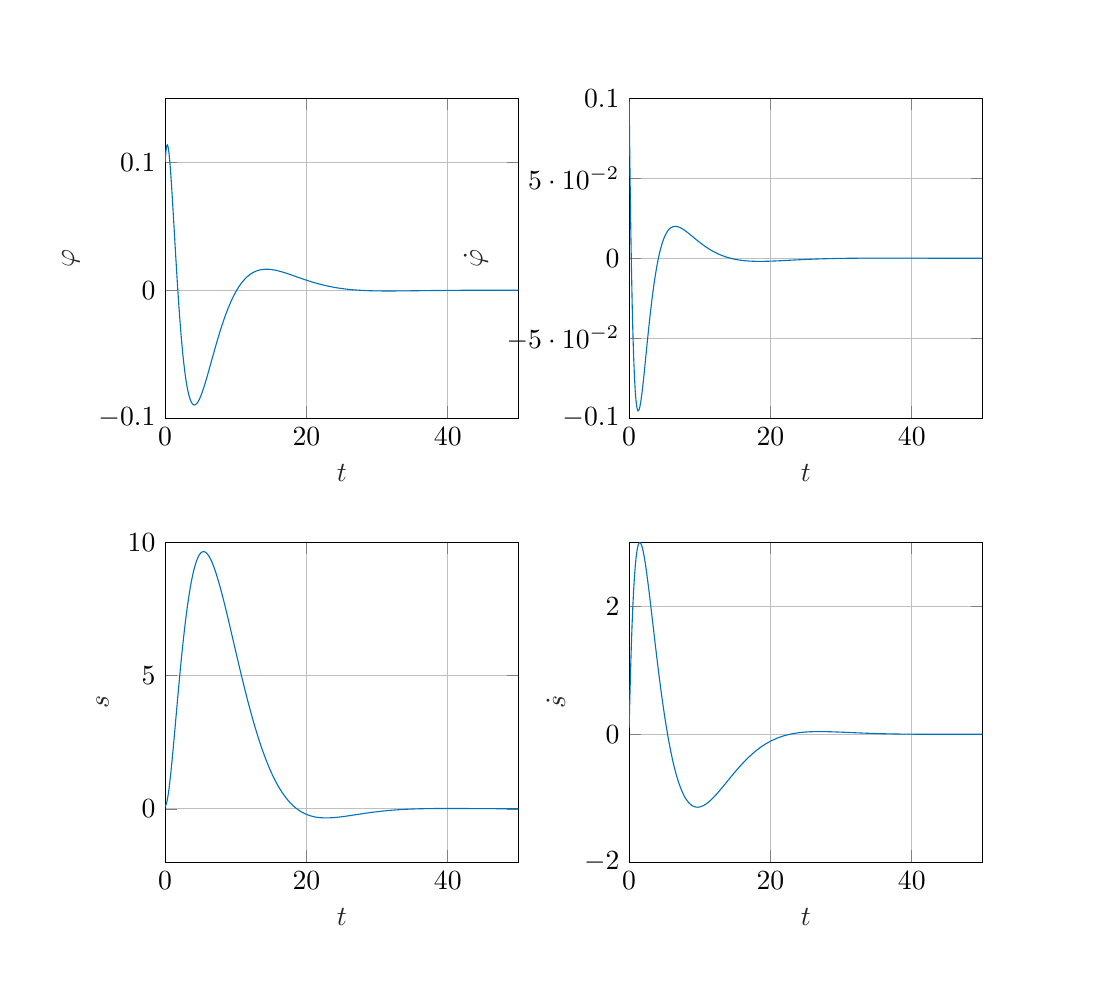
\begin{tikzpicture}

\begin{axis}[%
width=0.37\linewidth,
height=0.335\linewidth,
at={(0\linewidth,0.465\linewidth)},
scale only axis,
xmin=0,
xmax=50,
xlabel style={font=\color{white!15!black}},
xlabel={$t$},
ymin=-0.1,
ymax=0.15,
ylabel style={font=\color{white!15!black}},
ylabel={$\varphi$},
axis background/.style={fill=white},
xmajorgrids,
ymajorgrids
]
\addplot [color=mycolor1, forget plot]
  table[row sep=crcr]{%
0	0.1\\
0.000995243685935657	0.100099312801567\\
0.00199048737187131	0.100198202934099\\
0.00298573105780697	0.100296671094442\\
0.00398097474374263	0.100394717978522\\
0.00895719317342091	0.100878657549715\\
0.0139334116030992	0.101352169077539\\
0.0189096300327775	0.101815338527577\\
0.0238858484624558	0.102268251303793\\
0.0487669406108472	0.104381919350779\\
0.0736480327592386	0.106251659999478\\
0.09852912490763	0.107887531225803\\
0.123410217056021	0.10929927328696\\
0.224094033775409	0.112917615761137\\
0.324777850494796	0.113586015557344\\
0.425461667214183	0.111802259057869\\
0.52614548393357	0.108012738237674\\
0.636887572683258	0.101992268499682\\
0.747629661432947	0.0944428748377682\\
0.858371750182636	0.0857355166133191\\
0.969113838932324	0.0761982630834831\\
1.10490029877511	0.063780624741581\\
1.24068675861789	0.0509289620177077\\
1.37647321846068	0.037965669114613\\
1.51225967830346	0.0251683176815377\\
1.65853807055525	0.0118180188248237\\
1.80481646280705	-0.000916058019649089\\
1.95109485505884	-0.0129037516486061\\
2.09737324731064	-0.0240382222158139\\
2.22885595296554	-0.0332605681067052\\
2.36033865862045	-0.0417247518390192\\
2.49182136427535	-0.0494252121680808\\
2.62330406993026	-0.0563626171013431\\
2.80190445251268	-0.0645808944272592\\
2.98050483509509	-0.0714758868174342\\
3.15910521767751	-0.0771265348217437\\
3.33770560025993	-0.0816061680604652\\
3.52449863840961	-0.08512663495147\\
3.71129167655929	-0.0875726992411757\\
3.89808471470897	-0.0890538319107167\\
4.08487775285865	-0.0896687285560401\\
4.27286063586179	-0.0895096621413539\\
4.46084351886493	-0.0886715627061882\\
4.64882640186807	-0.087246016704649\\
4.83680928487121	-0.0853151917562865\\
5.03580321892655	-0.0828049466769832\\
5.23479715298189	-0.0798989431918482\\
5.43379108703723	-0.0766731203495882\\
5.63278502109258	-0.0731946434576746\\
5.90014717625525	-0.0682279962127354\\
6.16750933141793	-0.0630402526111606\\
6.4348714865806	-0.0577378860633029\\
6.70223364174328	-0.0524096212728846\\
7.04738138442873	-0.0456125920213146\\
7.39252912711419	-0.0390126187737777\\
7.73767686979964	-0.0326957958789793\\
8.08282461248509	-0.026731662429576\\
8.48888059796729	-0.0202338189423343\\
8.89493658344948	-0.0143192238016975\\
9.30099256893168	-0.00899600170177012\\
9.70704855441387	-0.00427227610038098\\
10.0956529840428	-0.000306884068997131\\
10.4842574136718	0.00314759099536919\\
10.8728618433008	0.00612074782475491\\
11.2614662729297	0.00864004571893327\\
11.6388531917555	0.0106807909778655\\
12.0162401105813	0.012356149872935\\
12.3936270294071	0.0136979560821352\\
12.7710139482329	0.0147359777125034\\
13.240890956687	0.0156475332147164\\
13.7107679651411	0.0161903345350407\\
14.1806449735952	0.0164172896507353\\
14.6505219820493	0.0163755257871648\\
15.1203397628241	0.0161085851711602\\
15.5901575435988	0.0156581477963036\\
16.0599753243736	0.0150609776191192\\
16.5297931051483	0.0143494445136309\\
17.0705885309305	0.0134260670394874\\
17.6113839567126	0.0124277441284066\\
18.1521793824948	0.0113870938005653\\
18.692974808277	0.0103313754622872\\
19.3280116497852	0.00910277808015657\\
19.9630484912934	0.00791260660467069\\
20.5980853328016	0.00678202736884502\\
21.2331221743098	0.00572695760198881\\
21.8594085044633	0.00477084920951434\\
22.4856948346167	0.00390329845459376\\
23.1119811647702	0.00312610643638458\\
23.7382674949237	0.00243936074203497\\
24.3395326061046	0.00186324696161723\\
24.9407977172854	0.00136424069356186\\
25.5420628284663	0.000937435800186874\\
26.1433279396471	0.000577817821129441\\
26.8306536861132	0.000242091056224359\\
27.5179794325793	-2.24488348638735e-05\\
28.2053051790453	-0.000225005146822555\\
28.8926309255114	-0.00037380925965327\\
29.5384980328083	-0.000471652715890812\\
30.1843651401053	-0.000535663443294649\\
30.8302322474022	-0.000571750167399793\\
31.4760993546992	-0.00058504545754821\\
32.2458242937129	-0.000577444105794036\\
33.0155492327266	-0.000551022404876297\\
33.7852741717403	-0.000511660542870428\\
34.554999110754	-0.00046402804496415\\
35.257249646804	-0.000416557210423802\\
35.9595001828541	-0.000367719446331404\\
36.6617507189041	-0.000319310208910461\\
37.3640012549541	-0.000272713007492988\\
37.9447491913198	-0.000236268645752506\\
38.5254971276855	-0.00020212600910106\\
39.1062450640513	-0.000170538686153175\\
39.686993000417	-0.000141675628581269\\
40.3438420767643	-0.000112415334719793\\
41.0006911531116	-8.66986977711515e-05\\
41.6575402294589	-6.44042396241359e-05\\
42.3143893058062	-4.53795328715038e-05\\
42.9136224684378	-3.07042687712106e-05\\
43.5128556310694	-1.83684528819027e-05\\
44.112088793701	-8.16027638969458e-06\\
44.7113219563325	1.22903950018005e-07\\
45.5043265706844	8.46330289076893e-06\\
46.2973311850362	1.42831340207299e-05\\
47.090335799388	1.80443332869522e-05\\
47.8833404137398	2.01302912618484e-05\\
48.4125053103048	2.07604686788881e-05\\
48.9416702068699	2.09042733959523e-05\\
49.4708351034349	2.06495709696673e-05\\
50	2.0074120518977e-05\\
};
\end{axis}

\begin{axis}[%
width=0.37\linewidth,
height=0.335\linewidth,
at={(0.486\linewidth,0.465\linewidth)},
scale only axis,
xmin=0,
xmax=50,
xlabel style={font=\color{white!15!black}},
xlabel={$t$},
ymin=-0.1,
ymax=0.1,
ylabel style={font=\color{white!15!black}},
ylabel={$\dot\varphi$},
axis background/.style={fill=white},
xmajorgrids,
ymajorgrids
]
\addplot [color=mycolor1, forget plot]
  table[row sep=crcr]{%
0	0.1\\
0.000995243685935657	0.0995749606179478\\
0.00199048737187131	0.0991506218707944\\
0.00298573105780697	0.0987269828369129\\
0.00398097474374263	0.0983040425958217\\
0.00895719317342091	0.0961997911440225\\
0.0139334116030992	0.0941128720978228\\
0.0189096300327775	0.0920431716813389\\
0.0238858484624558	0.0899905768238529\\
0.0487669406108472	0.0799802728235188\\
0.0736480327592386	0.0703810515313061\\
0.09852912490763	0.061179558953751\\
0.123410217056021	0.052362846193885\\
0.224094033775409	0.0203563309797967\\
0.324777850494796	-0.00631147586473885\\
0.425461667214183	-0.0283115988779764\\
0.52614548393357	-0.0462482890411035\\
0.636887572683258	-0.0619189762801853\\
0.747629661432947	-0.0739181293154147\\
0.858371750182636	-0.0827779057902851\\
0.969113838932324	-0.0889776181828309\\
1.10490029877511	-0.0935647877668988\\
1.24068675861789	-0.0954174522140939\\
1.37647321846068	-0.095079727201407\\
1.51225967830346	-0.0930362457935009\\
1.65853807055525	-0.0893951721540386\\
1.80481646280705	-0.0846322145458905\\
1.95109485505884	-0.0790716730657214\\
2.09737324731064	-0.0729983145776932\\
2.22885595296554	-0.0672918337071763\\
2.36033865862045	-0.0614718367316573\\
2.49182136427535	-0.055637682355943\\
2.62330406993026	-0.0498746750371651\\
2.80190445251268	-0.0422825641032805\\
2.98050483509509	-0.0350497738204687\\
3.15910521767751	-0.0282463028382197\\
3.33770560025993	-0.0219325752478694\\
3.52449863840961	-0.015891883147702\\
3.71129167655929	-0.010419380485584\\
3.89808471470897	-0.00550388021149719\\
4.08487775285865	-0.00113485663598583\\
4.27286063586179	0.00272952935073438\\
4.46084351886493	0.00609746038802059\\
4.64882640186807	0.00900429924350708\\
4.83680928487121	0.0114820556500364\\
5.03580321892655	0.0136738399142131\\
5.23479715298189	0.0154664045173343\\
5.43379108703723	0.0169008059739241\\
5.63278502109258	0.0180136592265607\\
5.90014717625525	0.0190626765059322\\
6.16750933141793	0.0196769551759885\\
6.4348714865806	0.0199301729890285\\
6.70223364174328	0.0198834280935563\\
7.04738138442873	0.0194676647188951\\
7.39252912711419	0.0187474909792741\\
7.73767686979964	0.0178067665956128\\
8.08282461248509	0.016713850707182\\
8.48888059796729	0.0153104981279777\\
8.89493658344948	0.0138405521184623\\
9.30099256893168	0.0123519066698601\\
9.70704855441387	0.0108883257481413\\
10.0956529840428	0.00954115303259962\\
10.4842574136718	0.00825783601042136\\
10.8728618433008	0.00704811305123964\\
11.2614662729297	0.00592115398846621\\
11.6388531917555	0.00491123150116509\\
12.0162401105813	0.00398381634554244\\
12.3936270294071	0.00313807338042319\\
12.7710139482329	0.00237299070499145\\
13.240890956687	0.00153011214512143\\
13.7107679651411	0.000801461818650842\\
14.1806449735952	0.00017902458668445\\
14.6505219820493	-0.000344471985525693\\
15.1203397628241	-0.000776712806889247\\
15.5901575435988	-0.00112707471508195\\
16.0599753243736	-0.00140408989783892\\
16.5297931051483	-0.00161556919153976\\
17.0705885309305	-0.00178759140675083\\
17.6113839567126	-0.00189422345281734\\
18.1521793824948	-0.00194588595893017\\
18.692974808277	-0.00195176489641811\\
19.3280116497852	-0.00191146007161648\\
19.9630484912934	-0.0018319041569466\\
20.5980853328016	-0.00172367021770045\\
21.2331221743098	-0.00159568941352807\\
21.8594085044633	-0.00145746095854859\\
22.4856948346167	-0.00131322881382938\\
23.1119811647702	-0.00116776005116024\\
23.7382674949237	-0.00102496523363163\\
24.3395326061046	-0.000893194684460964\\
24.9407977172854	-0.000768463627954892\\
25.5420628284663	-0.000652094899092364\\
26.1433279396471	-0.000545055888429743\\
26.8306536861132	-0.000434854965581634\\
27.5179794325793	-0.00033765951211328\\
28.2053051790453	-0.000253192426233435\\
28.8926309255114	-0.000181033270714676\\
29.5384980328083	-0.00012384966668982\\
30.1843651401053	-7.60722598266215e-05\\
30.8302322474022	-3.68279707921051e-05\\
31.4760993546992	-5.28961845326702e-06\\
32.2458242937129	2.33818041347714e-05\\
33.0155492327266	4.38436142310856e-05\\
33.7852741717403	5.75247171863717e-05\\
34.554999110754	6.56260056316047e-05\\
35.257249646804	6.90703720097403e-05\\
35.9595001828541	6.96013090463514e-05\\
36.6617507189041	6.79055548528292e-05\\
37.3640012549541	6.45538850226608e-05\\
37.9447491913198	6.08779167750643e-05\\
38.5254971276855	5.66470293236869e-05\\
39.1062450640513	5.20627645787905e-05\\
39.686993000417	4.72937830260364e-05\\
40.3438420767643	4.18517703831428e-05\\
41.0006911531116	3.6507928686119e-05\\
41.6575402294589	3.13817085642797e-05\\
42.3143893058062	2.65637543592593e-05\\
42.9136224684378	2.24906527321683e-05\\
43.5128556310694	1.87520116933994e-05\\
44.112088793701	1.53616912293977e-05\\
44.7113219563325	1.23256506480887e-05\\
45.5043265706844	8.848914676397e-06\\
46.2973311850362	5.95241761998882e-06\\
47.090335799388	3.58824140066311e-06\\
47.8833404137398	1.71058001239141e-06\\
48.4125053103048	7.03074268444788e-07\\
48.9416702068699	-1.30730248904573e-07\\
49.4708351034349	-8.08366359800529e-07\\
50	-1.34633149444259e-06\\
};
\end{axis}

\begin{axis}[%
width=0.37\linewidth,
height=0.335\linewidth,
at={(0\linewidth,0\linewidth)},
scale only axis,
xmin=0,
xmax=50,
xlabel style={font=\color{white!15!black}},
xlabel={$t$},
ymin=-2,
ymax=10,
ylabel style={font=\color{white!15!black}},
ylabel={$s$},
axis background/.style={fill=white},
xmajorgrids,
ymajorgrids
]
\addplot [color=mycolor1, forget plot]
  table[row sep=crcr]{%
0	0.1\\
0.000995243685935657	0.10010202326974\\
0.00199048737187131	0.100209040191858\\
0.00298573105780697	0.100321044545821\\
0.00398097474374263	0.10043803011688\\
0.00895719317342091	0.101097459110338\\
0.0139334116030992	0.101880489640779\\
0.0189096300327775	0.102786351346025\\
0.0238858484624558	0.103814277424799\\
0.0487669406108472	0.110758262611927\\
0.0736480327592386	0.120640875602343\\
0.09852912490763	0.133370201811392\\
0.123410217056021	0.14885638791006\\
0.224094033775409	0.237872649339107\\
0.324777850494796	0.365158920772861\\
0.425461667214183	0.525738015292224\\
0.52614548393357	0.715020590042202\\
0.636887572683258	0.951383518554234\\
0.747629661432947	1.21249935924537\\
0.858371750182636	1.4939083652772\\
0.969113838932324	1.79154498473746\\
1.10490029877511	2.17330046409105\\
1.24068675861789	2.56820933021459\\
1.37647321846068	2.97121598803908\\
1.51225967830346	3.37781842105841\\
1.65853807055525	3.81540457495146\\
1.80481646280705	4.24871847085598\\
1.95109485505884	4.67438435854154\\
2.09737324731064	5.08945857370313\\
2.22885595296554	5.45148857107638\\
2.36033865862045	5.80162455713786\\
2.49182136427535	6.13870355571687\\
2.62330406993026	6.46173811922733\\
2.80190445251268	6.87661688246589\\
2.98050483509509	7.26278997613067\\
3.15910521767751	7.61937385481459\\
3.33770560025993	7.94575363585322\\
3.52449863840961	8.25450949558466\\
3.71129167655929	8.53018806869957\\
3.89808471470897	8.77324355457808\\
4.08487775285865	8.9842642761968\\
4.27286063586179	9.16508032208343\\
4.46084351886493	9.3153235329545\\
4.64882640186807	9.43614448044453\\
4.83680928487121	9.5287313488522\\
5.03580321892655	9.59737709457299\\
5.23479715298189	9.63742860914343\\
5.43379108703723	9.65052603297624\\
5.63278502109258	9.63828622817177\\
5.90014717625525	9.58477429145845\\
6.16750933141793	9.49245139994211\\
6.4348714865806	9.36521567342708\\
6.70223364174328	9.20673643127101\\
7.04738138442873	8.9616411232428\\
7.39252912711419	8.67777614646835\\
7.73767686979964	8.36201047132396\\
8.08282461248509	8.02052315894731\\
8.48888059796729	7.59350943889317\\
8.89493658344948	7.14729333256111\\
9.30099256893168	6.6893805514141\\
9.70704855441387	6.22627319899107\\
10.0956529840428	5.78342547142537\\
10.4842574136718	5.34529519449703\\
10.8728618433008	4.9155173146516\\
11.2614662729297	4.49716912527647\\
11.6388531917555	4.1042513916568\\
12.0162401105813	3.72635922756817\\
12.3936270294071	3.3649614652476\\
12.7710139482329	3.02120908881699\\
13.240890956687	2.61912790719264\\
13.7107679651411	2.24657736697729\\
14.1806449735952	1.90390387831743\\
14.6505219820493	1.59107208072523\\
15.1203397628241	1.30767249333793\\
15.5901575435988	1.05273528634078\\
16.0599753243736	0.825121527115883\\
16.5297931051483	0.623573062115484\\
17.0705885309305	0.422016887977726\\
17.6113839567126	0.250622841322203\\
18.1521793824948	0.106830029846983\\
18.692974808277	-0.0118344513043169\\
19.3280116497852	-0.122404192779035\\
19.9630484912934	-0.205849932341952\\
20.5980853328016	-0.266055788408923\\
21.2331221743098	-0.306483886406232\\
21.8594085044633	-0.33010023678755\\
22.4856948346167	-0.340557942871079\\
23.1119811647702	-0.340458789309948\\
23.7382674949237	-0.332046305499219\\
24.3395326061046	-0.317973136979279\\
24.9407977172854	-0.29960280123817\\
25.5420628284663	-0.278246711317664\\
26.1433279396471	-0.255006530687726\\
26.8306536861132	-0.227306839811629\\
27.5179794325793	-0.19943655594312\\
28.2053051790453	-0.172239819070972\\
28.8926309255114	-0.146363316240291\\
29.5384980328083	-0.123664661987514\\
30.1843651401053	-0.102766857521249\\
30.8302322474022	-0.0838049562945337\\
31.4760993546992	-0.0668545280858389\\
32.2458242937129	-0.049297882683895\\
33.0155492327266	-0.0344799250024396\\
33.7852741717403	-0.0222082406102419\\
34.554999110754	-0.0122903246167967\\
35.257249646804	-0.00510634566538285\\
35.9595001828541	0.000526709219930879\\
36.6617507189041	0.00481373502993596\\
37.3640012549541	0.00793717088597201\\
37.9447491913198	0.00976491272826098\\
38.5254971276855	0.0110179942235598\\
39.1062450640513	0.011786359314875\\
39.686993000417	0.012150014794566\\
40.3438420767643	0.0121643170479846\\
41.0006911531116	0.0118496407637144\\
41.6575402294589	0.0112889160214246\\
42.3143893058062	0.0105516472665382\\
42.9136224684378	0.00977486953232039\\
43.5128556310694	0.00893823008516552\\
44.112088793701	0.00807290168265617\\
44.7113219563325	0.00720444930098524\\
45.5043265706844	0.00608512272067067\\
46.2973311850362	0.00502958609387494\\
47.090335799388	0.00406023233323889\\
47.8833404137398	0.0031921261152923\\
48.4125053103048	0.00267301265279224\\
48.9416702068699	0.00220222718792235\\
49.4708351034349	0.00177911775892512\\
50	0.00140253491910075\\
};
\end{axis}

\begin{axis}[%
width=0.37\linewidth,
height=0.335\linewidth,
at={(0.486\linewidth,0\linewidth)},
scale only axis,
xmin=0,
xmax=50,
xlabel style={font=\color{white!15!black}},
xlabel={$t$},
ymin=-2,
ymax=3,
ylabel style={font=\color{white!15!black}},
ylabel={$\dot s$},
axis background/.style={fill=white},
xmajorgrids,
ymajorgrids
]
\addplot [color=mycolor1, forget plot]
  table[row sep=crcr]{%
0	0.1\\
0.000995243685935657	0.105020644336302\\
0.00199048737187131	0.110035035500608\\
0.00298573105780697	0.115043179310796\\
0.00398097474374263	0.120045081579049\\
0.00895719317342091	0.144961172825939\\
0.0139334116030992	0.169722094078172\\
0.0189096300327775	0.194328565476145\\
0.0238858484624558	0.218781303659256\\
0.0487669406108472	0.338763857293658\\
0.0736480327592386	0.45500857605925\\
0.09852912490763	0.567601194595918\\
0.123410217056021	0.676625453067304\\
0.224094033775409	1.08304292298076\\
0.324777850494796	1.43742324718655\\
0.425461667214183	1.74440512283762\\
0.52614548393357	2.00828198133567\\
0.636887572683258	2.25342544028866\\
0.747629661432947	2.45586904433508\\
0.858371750182636	2.61992384847722\\
0.969113838932324	2.74957601371887\\
1.10490029877511	2.86692623001079\\
1.24068675861789	2.94392848792344\\
1.37647321846068	2.98588766739906\\
1.51225967830346	2.99763351633196\\
1.65853807055525	2.98140846075628\\
1.80481646280705	2.93966001494072\\
1.95109485505884	2.87643706401891\\
2.09737324731064	2.79539016427064\\
2.22885595296554	2.70996874349827\\
2.36033865862045	2.61466893619173\\
2.49182136427535	2.51124479077438\\
2.62330406993026	2.40128218653833\\
2.80190445251268	2.24395159136508\\
2.98050483509509	2.08004406249717\\
3.15910521767751	1.91203057551858\\
3.33770560025993	1.74210117870232\\
3.52449863840961	1.56432085105747\\
3.71129167655929	1.38803793043273\\
3.89808471470897	1.2146006523373\\
4.08487775285865	1.04518337503768\\
4.27286063586179	0.879705847406361\\
4.46084351886493	0.719931680248447\\
4.64882640186807	0.566407865673117\\
4.83680928487121	0.419587635881312\\
5.03580321892655	0.271838984696343\\
5.23479715298189	0.132172931515292\\
5.43379108703723	0.000707746089445183\\
5.63278502109258	-0.122492601513107\\
5.90014717625525	-0.27502277424939\\
6.16750933141793	-0.412962438869587\\
6.4348714865806	-0.536744746332658\\
6.70223364174328	-0.646819642557434\\
7.04738138442873	-0.769513159165808\\
7.39252912711419	-0.871791247975199\\
7.73767686979964	-0.955207705787406\\
8.08282461248509	-1.02118854527111\\
8.48888059796729	-1.0784457306217\\
8.89493658344948	-1.11614803490776\\
9.30099256893168	-1.13667875281092\\
9.70704855441387	-1.14217789855988\\
10.0956529840428	-1.13522946666636\\
10.4842574136718	-1.11811833388662\\
10.8728618433008	-1.09241788590856\\
11.2614662729297	-1.05955300956083\\
11.6388531917555	-1.02201486783972\\
12.0162401105813	-0.980050162604238\\
12.3936270294071	-0.93464699888591\\
12.7710139482329	-0.886690734224631\\
13.240890956687	-0.824602431101416\\
13.7107679651411	-0.761107340050477\\
14.1806449735952	-0.697337339272983\\
14.6505219820493	-0.634247209768186\\
15.1203397628241	-0.572633853888683\\
15.5901575435988	-0.513111941101218\\
16.0599753243736	-0.456174536088303\\
16.5297931051483	-0.402209144415345\\
17.0705885309305	-0.344137228659792\\
17.6113839567126	-0.290623602081273\\
18.1521793824948	-0.241790531011381\\
18.692974808277	-0.197676636395605\\
19.3280116497852	-0.151830420078815\\
19.9630484912934	-0.112138416747429\\
20.5980853328016	-0.0782364490294176\\
21.2331221743098	-0.0497416219960192\\
21.8594085044633	-0.0265156623071607\\
22.4856948346167	-0.00762996000280085\\
23.1119811647702	0.00739897909993885\\
23.7382674949237	0.0190182493931094\\
24.3395326061046	0.027366952851538\\
24.9407977172854	0.033364923068086\\
25.5420628284663	0.0373686238289273\\
26.1433279396471	0.0396953719368093\\
26.8306536861132	0.0406700236549927\\
27.5179794325793	0.0402319299734037\\
28.2053051790453	0.0387276533890011\\
28.8926309255114	0.0364458727558145\\
29.5384980328083	0.0338114555076786\\
30.1843651401053	0.0308811121975965\\
30.8302322474022	0.0277962093138841\\
31.4760993546992	0.024671286882618\\
32.2458242937129	0.0210207386981233\\
33.0155492327266	0.0175521682449218\\
33.7852741717403	0.0143410485880714\\
34.554999110754	0.0114394405838074\\
35.257249646804	0.00908653852364829\\
35.9595001828541	0.00701663593543956\\
36.6617507189041	0.00522361698270933\\
37.3640012549541	0.00369788247758646\\
37.9447491913198	0.00262733787617732\\
38.5254971276855	0.00171604127100753\\
39.1062450640513	0.00095095606349537\\
39.686993000417	0.000319390402253496\\
40.3438420767643	-0.00025015619011476\\
41.0006911531116	-0.000685425682655645\\
41.6575402294589	-0.00100531916841364\\
42.3143893058062	-0.00122665776703622\\
42.9136224684378	-0.00135587534860398\\
43.5128556310694	-0.00142783899634927\\
44.112088793701	-0.00145287126894545\\
44.7113219563325	-0.00143999817045954\\
45.5043265706844	-0.00137817231887173\\
46.2973311850362	-0.00128025887452984\\
47.090335799388	-0.00115967271646244\\
47.8833404137398	-0.00102684515581538\\
48.4125053103048	-0.000935463068459377\\
48.9416702068699	-0.000844304900410489\\
49.4708351034349	-0.000754942274959055\\
50	-0.000668651809049028\\
};
\end{axis}

\begin{axis}[%
width=1.104\linewidth,
height=0.982\linewidth,
at={(-0.144\linewidth,-0.108\linewidth)},
scale only axis,
xmin=0,
xmax=1,
ymin=0,
ymax=1,
axis line style={draw=none},
ticks=none,
axis x line*=bottom,
axis y line*=left
]
\end{axis}
\end{tikzpicture}%
	\caption{Поведение нелинеаризированной системы при действии линейного стабилизатора, решающего задачу оптимальной линейно-квадратичной стабилизации для заданных матриц функционала качества $Q = I \in \setR^4$, $R = 1$ из положения $x^0 = [0,\!1,\,0,\!1,\,0,\!1,\,0,\!1]$.}
\end{figure}

\begin{figure}[t]
	\centering
	% This file was created by matlab2tikz.
%
%The latest updates can be retrieved from
%  http://www.mathworks.com/matlabcentral/fileexchange/22022-matlab2tikz-matlab2tikz
%where you can also make suggestions and rate matlab2tikz.
%
\definecolor{mycolor1}{rgb}{0.00000,0.44700,0.74100}%
%
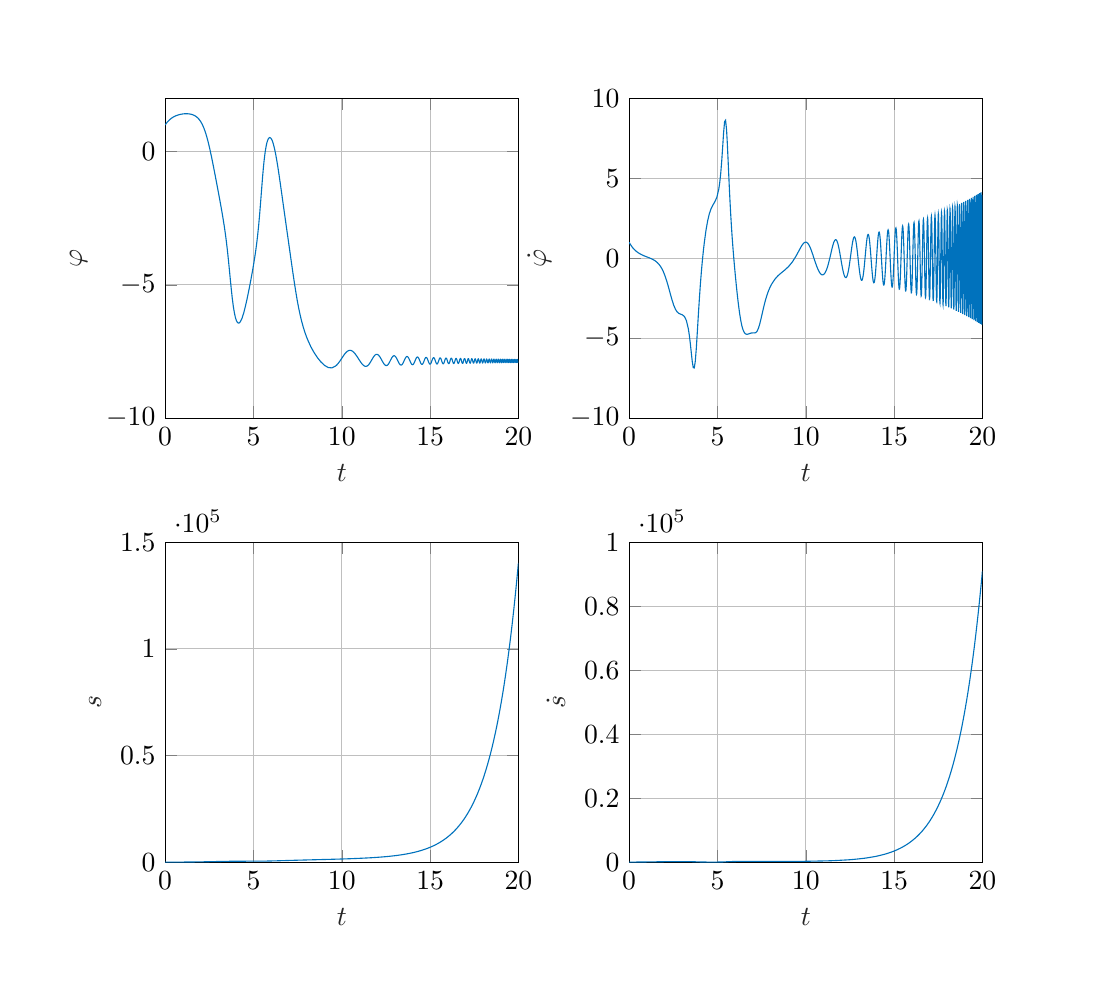
\begin{tikzpicture}

\begin{axis}[%
width=0.37\linewidth,
height=0.335\linewidth,
at={(0\linewidth,0.465\linewidth)},
scale only axis,
xmin=0,
xmax=20,
xlabel style={font=\color{white!15!black}},
xlabel={$t$},
ymin=-10,
ymax=2,
ylabel style={font=\color{white!15!black}},
ylabel={$\varphi$},
axis background/.style={fill=white},
xmajorgrids,
ymajorgrids
]
\addplot [color=mycolor1, forget plot]
  table[row sep=crcr]{%
0	1\\
0.000100639335033606	1.00010062867259\\
0.000201278670067211	1.00020123602355\\
0.000301918005100817	1.00030182205776\\
0.000402557340134422	1.00040238678011\\
0.00090575401530245	1.00090489088476\\
0.00140895069047048	1.00140686292468\\
0.00191214736563851	1.00190830350886\\
0.00241534404080653	1.00240921324547\\
0.00493132741664667	1.00490582044537\\
0.00744731079248681	1.00738924721225\\
0.00996329416832695	1.00985956865117\\
0.0124792775441671	1.01231685936571\\
0.0250591944233678	1.02441043244916\\
0.0376391113025685	1.03618914172114\\
0.0502190281817692	1.04766176409162\\
0.0627989450609699	1.05883679707691\\
0.114861963486122	1.10210084926028\\
0.166924981911275	1.14093553443053\\
0.218988000336427	1.17580441245237\\
0.27105101876158	1.20712636349349\\
0.3531926118804	1.25023367265807\\
0.435334204999219	1.28657292924076\\
0.517475798118039	1.31708348884678\\
0.599617391236859	1.34263322930146\\
0.681240080346691	1.36380757280753\\
0.762862769456523	1.38120985415484\\
0.844485458566355	1.39520470197824\\
0.926108147676188	1.4061111904624\\
1.00411789889559	1.41384746845452\\
1.08212765011499	1.41898954648624\\
1.1601374013344	1.42149717632161\\
1.2381471525538	1.42125530801761\\
1.30801821124067	1.41851947356247\\
1.37788926992754	1.41311559528568\\
1.44776032861441	1.4046660209374\\
1.51763138730128	1.39267853340684\\
1.59716717506405	1.37392242027045\\
1.67670296282682	1.3485568337793\\
1.75623875058959	1.31503767853056\\
1.83577453835236	1.27147111137513\\
1.9255866947371	1.20749370306614\\
2.01539885112183	1.12381352411428\\
2.10521100750657	1.01610743298258\\
2.1950231638913	0.880503713601269\\
2.2777508606761	0.728103109122475\\
2.3604785574609	0.547820093871777\\
2.4432062542457	0.340098896470827\\
2.52593395103049	0.107500527507069\\
2.62405192764858	-0.194651312383212\\
2.72216990426666	-0.516989372548251\\
2.82028788088475	-0.851741941438101\\
2.91840585750283	-1.19308044841589\\
3.0260210830503	-1.57191841391321\\
3.13363630859777	-1.95804043661807\\
3.24125153414524	-2.36259422252618\\
3.34886675969271	-2.80680807769225\\
3.4053515834801	-3.0660111075323\\
3.4618364072675	-3.35175861833528\\
3.51832123105489	-3.66905627701859\\
3.57480605484229	-4.01889468322976\\
3.63129087862969	-4.3970799889578\\
3.68777570241708	-4.78565694566648\\
3.74426052620448	-5.16233684295979\\
3.80074534999187	-5.50532975870401\\
3.8597827958403	-5.80807741320414\\
3.91882024168872	-6.04795980677126\\
3.97785768753714	-6.22543070384057\\
4.03689513338557	-6.34456072818264\\
4.0906880435324	-6.4082486067293\\
4.14448095367923	-6.43418728879155\\
4.19827386382606	-6.4265089931725\\
4.25206677397289	-6.38899210814341\\
4.34893452842244	-6.25686728425833\\
4.44580228287199	-6.05729491839291\\
4.54267003732154	-5.80690761424975\\
4.6395377917711	-5.52017427537912\\
4.74771052145859	-5.1713162837993\\
4.85588325114608	-4.80034240126796\\
4.96405598083357	-4.40409764237237\\
5.07222871052106	-3.96685518311928\\
5.12755667253839	-3.71798445702358\\
5.18288463455573	-3.4417672823718\\
5.23821259657306	-3.12894003161094\\
5.2935405585904	-2.77075129354442\\
5.34886852060773	-2.35974715742331\\
5.40419648262506	-1.9040176509133\\
5.4595244446424	-1.42669635807861\\
5.51485240665973	-0.961830096812303\\
5.55441616049067	-0.65890948796173\\
5.59397991432161	-0.390122734913899\\
5.63354366815254	-0.159340529704941\\
5.67310742198348	0.0327728278428391\\
5.71267117581442	0.188493852203433\\
5.75223492964535	0.311024366319675\\
5.79179868347629	0.403402392644615\\
5.83136243730723	0.468545374180275\\
5.87811828864509	0.51400241080036\\
5.92487413998296	0.528205049626647\\
5.97162999132083	0.513630469889815\\
6.0183858426587	0.472373082013214\\
6.06514169399657	0.406084543969494\\
6.11189754533443	0.316071214666748\\
6.1586533966723	0.203768493604327\\
6.20540924801017	0.0708064659860111\\
6.26402010980554	-0.122260949943435\\
6.32263097160091	-0.340589585570309\\
6.38124183339628	-0.579483513892535\\
6.43985269519164	-0.834207436953819\\
6.5138827604118	-1.17138902814268\\
6.58791282563196	-1.51868547509556\\
6.66194289085212	-1.87026333593375\\
6.73597295607228	-2.22209903611932\\
6.8213190911498	-2.62527894691551\\
6.90666522622733	-3.02580887295711\\
6.99201136130486	-3.42464041121652\\
7.07735749638238	-3.82305128849562\\
7.158032282141	-4.19989932114478\\
7.23870706789961	-4.57258325706111\\
7.31938185365823	-4.93409716396165\\
7.40005663941684	-5.27627403085591\\
7.48073142517546	-5.59087764985826\\
7.56140621093407	-5.87454828665696\\
7.64208099669269	-6.12707133010653\\
7.7227557824513	-6.35024350041464\\
7.80743172089708	-6.55684582671198\\
7.89210765934286	-6.73944608316766\\
7.97678359778864	-6.90184952262648\\
8.06145953623442	-7.04737357400477\\
8.248921381391	-7.32133268519853\\
8.43638322654757	-7.5447322010819\\
8.62384507170415	-7.73087618000135\\
8.81130691686072	-7.88510065732964\\
9.02163025677818	-8.01891173250231\\
9.23195359669565	-8.10021109894994\\
9.44227693661311	-8.1136457249941\\
9.65260027653057	-8.04411097880737\\
9.71956708495155	-8.00262069669842\\
9.78653389337253	-7.95245535487137\\
9.85350070179351	-7.89475607665998\\
9.92046751021449	-7.83130183686835\\
9.98743431863547	-7.76442185711068\\
10.0544011270565	-7.69711237047226\\
10.1213679354774	-7.63260538286781\\
10.1883347438984	-7.57409840061367\\
10.2574161214033	-7.52319459925684\\
10.3264974989082	-7.48482525873173\\
10.3955788764131	-7.46117570898896\\
10.464660253918	-7.4533373077117\\
10.5337416314229	-7.46147939408284\\
10.6028230089278	-7.4852406838973\\
10.6719043864327	-7.52346594577986\\
10.7409857639376	-7.57415971532063\\
10.797724388208	-7.62332334225618\\
10.8544630124784	-7.67761051306705\\
10.9112016367488	-7.73520692901841\\
10.9679402610191	-7.79413517412475\\
11.0323692086966	-7.86003852437035\\
11.0967981563741	-7.92159156141577\\
11.1612271040515	-7.9752921486633\\
11.225656051729	-8.01777571593565\\
11.2829909721646	-8.0436349994805\\
11.3403258926002	-8.05595107542862\\
11.3976608130357	-8.05311273576989\\
11.4549957334713	-8.03449423388914\\
11.4996184181378	-8.00926058854251\\
11.5442411028043	-7.97524720228819\\
11.5888637874709	-7.93363264327412\\
11.6334864721374	-7.88619869665459\\
11.6781091568039	-7.83519452172037\\
11.7227318414704	-7.78332922671012\\
11.767354526137	-7.73350098610047\\
11.8119772108035	-7.68857337856231\\
11.8567770115385	-7.65106633248524\\
11.9015768122735	-7.62360540448023\\
11.9463766130085	-7.60800896347076\\
11.9911764137435	-7.60518448961095\\
12.0350810389572	-7.61491631041636\\
12.078985664171	-7.63666304007923\\
12.1228902893848	-7.66934581015596\\
12.1667949145986	-7.7110902389053\\
12.2027433089555	-7.75032975118514\\
12.2386917033124	-7.79255115534725\\
12.2746400976693	-7.83607373953221\\
12.3105884920262	-7.8791100256507\\
12.3491431802909	-7.92265953349234\\
12.3876978685556	-7.96119773347073\\
12.4262525568202	-7.99249062794261\\
12.4648072450849	-8.01463407946778\\
12.5002952050204	-8.02560999229253\\
12.535783164956	-8.02654976886666\\
12.5712711248915	-8.01697840577984\\
12.606759084827	-7.99711167527072\\
12.6422470447626	-7.96777971300094\\
12.6777350046981	-7.93036109521557\\
12.7132229646336	-7.88690009123377\\
12.7487109245691	-7.84009130966617\\
12.7791600450121	-7.79960281930754\\
12.8096091654551	-7.76097789539699\\
12.8400582858981	-7.72624598309133\\
12.870507406341	-7.69721567108634\\
12.9058119698418	-7.67263989429386\\
12.9411165333426	-7.65970181866206\\
12.9764210968433	-7.65954855535393\\
13.0117256603441	-7.67215475601534\\
13.0400221599409	-7.69085191786708\\
13.0683186595376	-7.71641827332297\\
13.0966151591344	-7.74774226416101\\
13.1249116587312	-7.78337865864198\\
13.1514911766817	-7.81929013291355\\
13.1780706946321	-7.85601802753384\\
13.2046502125826	-7.89195854610151\\
13.2312297305331	-7.92550839728799\\
13.2601626364332	-7.95752298976198\\
13.2890955423332	-7.98292395323578\\
13.3180284482332	-8.00004172753709\\
13.3469613541333	-8.0077158208841\\
13.3715874271246	-8.00629198058666\\
13.3962135001159	-7.99735008735617\\
13.4208395731072	-7.98108836295141\\
13.4454656460985	-7.95814260248002\\
13.4700917190899	-7.92950898336724\\
13.4947177920812	-7.89649071489793\\
13.5193438650725	-7.86069098457619\\
13.5439699380638	-7.82395119936658\\
13.5673398362303	-7.78999332133508\\
13.5907097343968	-7.75865682423335\\
13.6140796325634	-7.73154399821807\\
13.6374495307299	-7.71001017670535\\
13.6589807715322	-7.69605167521886\\
13.6805120123344	-7.6884327199412\\
13.7020432531367	-7.68754623229235\\
13.723574493939	-7.69343686479005\\
13.7451057347413	-7.70585248553807\\
13.7666369755436	-7.72432713726681\\
13.7881682163458	-7.7481125896007\\
13.8096994571481	-7.77617935462195\\
13.8304267111029	-7.80609479249531\\
13.8511539650576	-7.83761212682597\\
13.8718812190124	-7.86940661152579\\
13.8926084729671	-7.90011943423326\\
13.9147000097324	-7.93016414241778\\
13.9367915464976	-7.95584703799925\\
13.9588830832629	-7.97573074542758\\
13.9809746200281	-7.98869941949661\\
14.0027870917886	-7.99395451480212\\
14.0245995635492	-7.99118713807503\\
14.0464120353097	-7.98032948734099\\
14.0682245070702	-7.96187617237677\\
14.0900369788307	-7.93678052667021\\
14.1118494505912	-7.9063490621703\\
14.1336619223517	-7.87228510529913\\
14.1554743941123	-7.83663483599908\\
14.1743578255751	-7.80620223986633\\
14.1932412570379	-7.77769784420801\\
14.2121246885008	-7.75251685473165\\
14.2310081199636	-7.73186806533644\\
14.2490081448628	-7.71732263198464\\
14.267008169762	-7.70851780792472\\
14.2850081946613	-7.70590321964589\\
14.3030082195605	-7.70959724362592\\
14.3210082444597	-7.71943325895487\\
14.3390082693589	-7.73503926374943\\
14.3570082942581	-7.7557671652341\\
14.3750083191574	-7.78068892358729\\
14.3920562821893	-7.80713747872943\\
14.4091042452212	-7.8352611457066\\
14.4261522082531	-7.86388996584188\\
14.443200171285	-7.89181668044097\\
14.4613772001078	-7.91947934702264\\
14.4795542289306	-7.94354367492382\\
14.4977312577534	-7.9627163532617\\
14.5159082865762	-7.97597519889591\\
14.5342462046075	-7.98260974964869\\
14.5525841226387	-7.98193069479403\\
14.5709220406699	-7.97380190795977\\
14.5892599587012	-7.95860016547213\\
14.6075978767324	-7.93712076198126\\
14.6259357947636	-7.91046982176613\\
14.6442737127949	-7.88011825370799\\
14.6626116308261	-7.84786124813874\\
14.6785151598573	-7.81986580625109\\
14.6944186888886	-7.79322379098228\\
14.7103222179198	-7.76920815580185\\
14.726225746951	-7.74894775128\\
14.7455153818685	-7.73073414708818\\
14.7648050167859	-7.72083362852817\\
14.7840946517034	-7.72008726246691\\
14.8033842866208	-7.72851320533224\\
14.8193522482764	-7.74198578204787\\
14.8353202099321	-7.76074508226679\\
14.8512881715877	-7.78391864747168\\
14.8672561332433	-7.81036310473957\\
14.8819519595868	-7.83645564133168\\
14.8966477859303	-7.86309065611683\\
14.9113436122737	-7.88910897696505\\
14.9260394386172	-7.91337209763827\\
14.9421319316524	-7.93666519525439\\
14.9582244246877	-7.95521921864955\\
14.9743169177229	-7.96791930294147\\
14.9904094107581	-7.9740221179985\\
15.004551163206	-7.97361621180024\\
15.0186929156539	-7.96770785891699\\
15.0328346681018	-7.95646669826673\\
15.0469764205498	-7.94035726503545\\
15.0611181729977	-7.92008067345969\\
15.0752599254456	-7.89652135614911\\
15.0894016778935	-7.87074855160119\\
15.1035434303414	-7.8439762363812\\
15.1173989223857	-7.81801347513643\\
15.1312544144301	-7.79356259007095\\
15.1451099064744	-7.77180204336105\\
15.1589653985187	-7.75375919752928\\
15.172526710212	-7.74052231940552\\
15.1860880219052	-7.73233369290873\\
15.1996493335984	-7.72962067244528\\
15.2132106452917	-7.73250506602121\\
15.2267719569849	-7.74084568774389\\
15.2403332686781	-7.7543127988425\\
15.2538945803714	-7.77232233238226\\
15.2674558920646	-7.79403170699726\\
15.2801060223518	-7.81671468611439\\
15.2927561526391	-7.84079854498458\\
15.3054062829263	-7.86527901958722\\
15.3180564132135	-7.88912668092791\\
15.3315611141882	-7.91274861865509\\
15.3450658151628	-7.93328160967402\\
15.3585705161374	-7.94964776622871\\
15.372075217112	-7.9610062527901\\
15.386074510251	-7.9668617827383\\
15.40007380339	-7.96623722118139\\
15.4140730965291	-7.95904184861495\\
15.4280723896681	-7.94564696163487\\
15.4420716828071	-7.92679333891586\\
15.4560709759461	-7.90348146829764\\
15.4700702690852	-7.87701776725032\\
15.4840695622242	-7.84897404664588\\
15.496152402728	-7.82480798065391\\
15.5082352432317	-7.80184146088101\\
15.5203180837355	-7.78114755468913\\
15.5324009242393	-7.76367480759811\\
15.5472559317962	-7.74774275183061\\
15.5621109393531	-7.73909500960606\\
15.57696594691	-7.73846053792694\\
15.5918209544669	-7.7458472869296\\
15.6041576236101	-7.75768371640319\\
15.6164942927534	-7.77415900208474\\
15.6288309618966	-7.79449732330391\\
15.6411676310398	-7.81768565498351\\
15.6525060682938	-7.84051041379111\\
15.6638445055477	-7.86378592622831\\
15.6751829428017	-7.88650233791518\\
15.6865213800557	-7.90767335505502\\
15.6989797156882	-7.9280587144825\\
15.7114380513208	-7.94429932359934\\
15.7238963869533	-7.95544178541465\\
15.7363547225858	-7.96085925006051\\
15.7473759168046	-7.96061182964229\\
15.7583971110234	-7.9555531179113\\
15.7694183052422	-7.94584003428909\\
15.7804394994611	-7.93188118897406\\
15.7914606936799	-7.91428555732777\\
15.8024818878987	-7.89381322656734\\
15.8135030821175	-7.87137731491504\\
15.8245242763363	-7.84800970347043\\
15.8354225590621	-7.82505349291795\\
15.8463208417879	-7.80333073704469\\
15.8572191245138	-7.78387073038068\\
15.8681174072396	-7.76757612770509\\
15.8815088767169	-7.75295511124911\\
15.8949003461942	-7.7453722542441\\
15.9082918156714	-7.74548180346931\\
15.9216832851487	-7.75323678549372\\
15.9326177050092	-7.76483203377657\\
15.9435521248698	-7.78063879108867\\
15.9544865447303	-7.79992579897607\\
15.9654209645908	-7.82175471499384\\
15.9756095934322	-7.84344028223224\\
15.9857982222735	-7.86547511090662\\
15.9959868511149	-7.88690116833227\\
16.0061754799563	-7.90678824156861\\
16.0174258808305	-7.92592431879404\\
16.0286762817047	-7.94102788126509\\
16.0399266825789	-7.95120749318568\\
16.0511770834532	-7.95589188313321\\
16.0610658987087	-7.95524421275676\\
16.0709547139642	-7.95008730738954\\
16.0808435292198	-7.94058987583221\\
16.0907323444753	-7.92715193766524\\
16.1006211597309	-7.91035664780757\\
16.1105099749864	-7.89092418247584\\
16.120398790242	-7.86971158454821\\
16.1302876054975	-7.84767990792461\\
16.1401470581209	-7.82590207394401\\
16.1500065107444	-7.80533653265239\\
16.1598659633678	-7.78695545202852\\
16.1697254159912	-7.7716083273222\\
16.1819127978002	-7.75784047939606\\
16.1941001796092	-7.7508509473361\\
16.2062875614183	-7.75125030943134\\
16.2184749432273	-7.75896917609021\\
16.2283504170631	-7.77018842549574\\
16.238225890899	-7.78534871525232\\
16.2481013647348	-7.80375182756748\\
16.2579768385706	-7.8245089304786\\
16.2672247914286	-7.84518458876076\\
16.2764727442866	-7.86615219515543\\
16.2857206971446	-7.8864997362064\\
16.2949686500026	-7.90534489679155\\
16.3052118235449	-7.92348043786641\\
16.3154549970871	-7.93772405539638\\
16.3256981706294	-7.94723484723174\\
16.3359413441717	-7.95148221692415\\
16.3449228948705	-7.9506731951158\\
16.3539044455693	-7.9455927953304\\
16.3628859962681	-7.93641216973865\\
16.3718675469669	-7.92351893175015\\
16.3808490976657	-7.90747143549565\\
16.3898306483645	-7.88895487025767\\
16.3988121990633	-7.86878025160713\\
16.4077937497621	-7.84785299978753\\
16.416792574534	-7.82708226131002\\
16.4257913993059	-7.80748191052747\\
16.4347902240778	-7.7899758523943\\
16.4437890488497	-7.7753701656347\\
16.4549439838876	-7.76225238445923\\
16.4660989189255	-7.7556331114446\\
16.4772538539635	-7.75609098215841\\
16.4884087890014	-7.76355196544595\\
16.4974338921827	-7.77432230538189\\
16.506458995364	-7.78884266569453\\
16.5154840985453	-7.80644427943863\\
16.5245092017267	-7.8262781544358\\
16.5329728147682	-7.84604887730255\\
16.5414364278097	-7.86608763411665\\
16.5499000408513	-7.88552357582844\\
16.5583636538928	-7.90351565533691\\
16.567750821481	-7.92084346847684\\
16.5771379890692	-7.93444114498296\\
16.5865251566573	-7.94350937885859\\
16.5959123242455	-7.94754664864444\\
16.6041494770369	-7.94675629900582\\
16.6123866298282	-7.94188571085237\\
16.6206237826196	-7.93310161544454\\
16.6288609354109	-7.92077618290652\\
16.6370980882023	-7.90544329199118\\
16.6453352409937	-7.88775619035551\\
16.653572393785	-7.86848647099024\\
16.6618095465764	-7.84849411403626\\
16.6700825047718	-7.82859444526099\\
16.6783554629672	-7.80980398256589\\
16.6866284211627	-7.79300529703018\\
16.6949013793581	-7.77896883602387\\
16.7051521458485	-7.76632798488055\\
16.7154029123389	-7.75988091353244\\
16.7256536788293	-7.76018451116393\\
16.7359044453197	-7.76717670474017\\
16.7442396992767	-7.77742349404808\\
16.7525749532337	-7.79129865993135\\
16.7609102071908	-7.80815995306292\\
16.7692454611478	-7.82718995383159\\
16.777043879309	-7.84613502147341\\
16.7848422974702	-7.86535449754238\\
16.7926407156314	-7.88401497607847\\
16.8004391337926	-7.90131136104621\\
16.8090845655159	-7.91799362904438\\
16.8177299972392	-7.93113069775722\\
16.8263754289625	-7.93995752730041\\
16.8350208606859	-7.94399164517517\\
16.8426386279751	-7.94338879633195\\
16.8502563952644	-7.93885819578995\\
16.8578741625537	-7.93055582763389\\
16.865491929843	-7.91883527416231\\
16.8731096971323	-7.90420559081565\\
16.8807274644216	-7.88728995045426\\
16.8883452317109	-7.86882534774595\\
16.8959629990001	-7.84963416079712\\
16.9036139294144	-7.83049624030217\\
16.9112648598286	-7.8123853610787\\
16.9189157902429	-7.79614823923357\\
16.9265667206571	-7.7825261778645\\
16.9360095495064	-7.77020233696402\\
16.9454523783557	-7.76373548264861\\
16.954895207205	-7.76367014197535\\
16.9643380360542	-7.76997245045415\\
16.9721134011385	-7.77960425484042\\
16.9798887662227	-7.79281009630235\\
16.987664131307	-7.80897195153343\\
16.9954394963912	-7.82729625543959\\
17.0026655309991	-7.84547195091566\\
17.009891565607	-7.8639581111784\\
17.0171176002149	-7.88195602013773\\
17.0243436348227	-7.89869223044274\\
17.032334723359	-7.91486962136097\\
17.0403258118952	-7.92771355656385\\
17.0483169004314	-7.936487214399\\
17.0563079889676	-7.94071828102925\\
17.0634073402217	-7.94047493463507\\
17.0705066914759	-7.93642114938555\\
17.07760604273	-7.92869578738752\\
17.0847053939841	-7.91763052898993\\
17.0918047452383	-7.90370895529767\\
17.0989040964924	-7.88752553833507\\
17.1060034477465	-7.86978681952192\\
17.1131027990007	-7.85128455495812\\
17.1202132497858	-7.83282214384144\\
17.1273237005709	-7.81528290319565\\
17.134434151356	-7.79948192964339\\
17.1415446021411	-7.78613670396853\\
17.1502562530781	-7.77398482671969\\
17.158967904015	-7.76732124382948\\
17.1676795549519	-7.76668622272485\\
17.1763912058889	-7.77208803815555\\
17.183714325741	-7.78100217060499\\
17.1910374455932	-7.79350106643177\\
17.1983605654454	-7.80898926073695\\
17.2056836852976	-7.82668965962184\\
17.2124116530922	-7.84413525146675\\
17.2191396208867	-7.86195404426155\\
17.2258675886813	-7.87937989375807\\
17.2325955564758	-7.89566751683712\\
17.2400022894173	-7.91145443366749\\
17.2474090223588	-7.92414455440592\\
17.2548157553003	-7.93302464396841\\
17.2622224882419	-7.93762552547272\\
17.2688889620112	-7.93790067045718\\
17.2755554357805	-7.93444887982875\\
17.2822219095498	-7.92738608385272\\
17.2888883833191	-7.91701946948699\\
17.2955548570884	-7.90380727143727\\
17.3022213308577	-7.88831733809399\\
17.308887804627	-7.87123050653117\\
17.3155542783963	-7.85331532991574\\
17.3221901055366	-7.83546444854504\\
17.328825932677	-7.81841717688132\\
17.3354617598173	-7.80296002065158\\
17.3420975869576	-7.78979042258797\\
17.3501500549749	-7.77770402514338\\
17.3582025229921	-7.77072357840199\\
17.3662549910093	-7.76939028837551\\
17.3743074590266	-7.77376164808253\\
17.3812633391027	-7.7818803852181\\
17.3882192191788	-7.79364620020174\\
17.395175099255	-7.80848500132027\\
17.4021309793311	-7.8256298141239\\
17.4084227113778	-7.84238076635914\\
17.4147144434244	-7.85958358702706\\
17.421006175471	-7.87650261849577\\
17.4272979075176	-7.89241789081795\\
17.434182608289	-7.90788698227535\\
17.4410673090603	-7.92050567500142\\
17.4479520098317	-7.92958143756133\\
17.454836710603	-7.9346446371323\\
17.4611440879004	-7.93553366705692\\
17.4674514651978	-7.93274761787963\\
17.4737588424952	-7.92637616037855\\
17.4800662197926	-7.91670195682923\\
17.48637359709	-7.90416050621429\\
17.4926809743874	-7.88929739552087\\
17.4989883516847	-7.87277440190265\\
17.5052957289821	-7.85534562151085\\
17.5115125473571	-7.83806074506606\\
17.517729365732	-7.82146197090307\\
17.523946184107	-7.80630920909199\\
17.530163002482	-7.79328159582097\\
17.5376362255223	-7.7812305230541\\
17.5451094485626	-7.77392969691205\\
17.5525826716029	-7.77192174020829\\
17.5600558946433	-7.77530915245247\\
17.5666991317891	-7.78264673759586\\
17.573342368935	-7.79370972054492\\
17.5799856060808	-7.80794415901843\\
17.5866288432267	-7.82458970914613\\
17.5925376579821	-7.84069779575004\\
17.5984464727376	-7.85733206385012\\
17.6043552874931	-7.87378457914356\\
17.6102641022486	-7.88935824692694\\
17.616689389498	-7.90452878792444\\
17.6231146767474	-7.91707505901129\\
17.6295399639969	-7.92632398290232\\
17.6359652512463	-7.93180632469174\\
17.641971372891	-7.93327665743329\\
17.6479774945357	-7.93110100846997\\
17.6539836161803	-7.92534435130285\\
17.659989737825	-7.91626883233566\\
17.6659958594697	-7.90429300780878\\
17.6720019811144	-7.88994704967626\\
17.6780081027591	-7.87388162438049\\
17.6840142244037	-7.8568450207521\\
17.6898612452845	-7.84008764505067\\
17.6957082661652	-7.82392543212505\\
17.7015552870459	-7.80909327907166\\
17.7074023079266	-7.79625192786837\\
17.714385603669	-7.78429653447252\\
17.7213688994113	-7.77680813901633\\
17.7283521951536	-7.77432660864776\\
17.735335490896	-7.77698451838397\\
17.741684870856	-7.783693668178\\
17.7480342508161	-7.79417089399525\\
17.7543836307762	-7.80788040556986\\
17.7607330107363	-7.82406972651966\\
17.7663049301025	-7.8396142258699\\
17.7718768494688	-7.85573329635507\\
17.777448768835	-7.87174314861598\\
17.7830206882012	-7.88696743552423\\
17.7890508494389	-7.90181750070549\\
17.7950810106766	-7.91421828900231\\
17.8011111719143	-7.92351565146887\\
17.807141333152	-7.92924489636388\\
17.8128772692463	-7.93112127421684\\
17.8186132053407	-7.92938057509107\\
17.824349141435	-7.92407000575623\\
17.8300850775293	-7.91543775901013\\
17.8358210136237	-7.90389147852776\\
17.841556949718	-7.88995151441552\\
17.8472928858124	-7.87426190985875\\
17.8530288219067	-7.85756810966851\\
17.8585498771667	-7.8412962420697\\
17.8640709324266	-7.8255663609729\\
17.8695919876865	-7.81109027584352\\
17.8751130429465	-7.79850994415818\\
17.8816897742058	-7.78674889035047\\
17.8882665054652	-7.77925836672688\\
17.8948432367245	-7.77656988813114\\
17.9014199679839	-7.77882872590554\\
17.9074737751274	-7.78513233985131\\
17.913527582271	-7.7951824955674\\
17.9195813894145	-7.80845898170173\\
17.9256351965581	-7.82422174544275\\
17.930908575703	-7.83929043113169\\
17.9361819548479	-7.8549498348648\\
17.9414553339928	-7.87053680014696\\
17.9467287131377	-7.88539397049988\\
17.9524220574687	-7.89989624842873\\
17.9581154017997	-7.91206622694543\\
17.9638087461308	-7.92126794789389\\
17.9695020904618	-7.92704555817174\\
17.9749744850704	-7.92910574271301\\
17.9804468796791	-7.9276009871872\\
17.9859192742877	-7.92256930661154\\
17.9913916688963	-7.91425001310189\\
17.9968640635049	-7.90304200785955\\
18.0023364581135	-7.88945621232593\\
18.0078088527222	-7.8741275501249\\
18.0132812473308	-7.85779308931208\\
18.0185136161325	-7.84196325929747\\
18.0237459849342	-7.82664709557584\\
18.028978353736	-7.81253566294842\\
18.0342107225377	-7.80025288960956\\
18.040440614117	-7.78874345711376\\
18.0466705056964	-7.78136425483239\\
18.0529003972757	-7.77863527448018\\
18.059130288855	-7.78070417687156\\
18.0648950028344	-7.78675368764742\\
18.0706597168137	-7.79648612058462\\
18.0764244307931	-7.80939488703555\\
18.0821891447724	-7.82475555123022\\
18.0871952754586	-7.8394127549626\\
18.0922014061448	-7.8546578070945\\
18.097207536831	-7.86984568029416\\
18.1022136675171	-7.88433654839262\\
18.1076139110201	-7.89848766624606\\
18.1130141545231	-7.91038738248491\\
18.1184143980261	-7.91941681132092\\
18.1238146415291	-7.92513086116916\\
18.129030937539	-7.92723912810559\\
18.134247233549	-7.92585362554971\\
18.1394635295589	-7.92100838805626\\
18.1446798255688	-7.91293604550176\\
18.1498961215788	-7.90202656382078\\
18.1551124175887	-7.88877987539289\\
18.1603287135986	-7.87381808631011\\
18.1655450096085	-7.85786407607331\\
18.1705189405597	-7.84243868816581\\
18.1754928715108	-7.82750734889988\\
18.1804668024619	-7.81374247025348\\
18.185440733413	-7.80175140866615\\
18.1913626809683	-7.79049932576406\\
18.1972846285236	-7.78326008790503\\
18.2032065760789	-7.7805417165428\\
18.2091285236342	-7.78249116042051\\
18.2146241615657	-7.78834367191801\\
18.2201197994971	-7.79780558315362\\
18.2256154374286	-7.81038277940719\\
18.23111107536	-7.82536682069147\\
18.2358759623131	-7.8396512768929\\
18.2406408492662	-7.85451553346047\\
18.2454057362193	-7.86933108426058\\
18.2501706231724	-7.88347433724647\\
18.2553087976448	-7.89729112110337\\
18.2604469721171	-7.90892322893497\\
18.2655851465894	-7.91776761851846\\
18.2707233210617	-7.92338988999037\\
18.2757014808253	-7.9255049522\\
18.2806796405889	-7.92420003452657\\
18.2856578003525	-7.91950684133268\\
18.2906359601161	-7.9116521541007\\
18.2956141198798	-7.90101720680762\\
18.3005922796434	-7.88809084140755\\
18.305570439407	-7.87348170104156\\
18.3105485991706	-7.85789728465497\\
18.3152888411157	-7.84284587978771\\
18.3200290830609	-7.82827183302634\\
18.324769325006	-7.81483045834147\\
18.3295095669512	-7.80311384116412\\
18.3351532829551	-7.79210704570619\\
18.3407969989589	-7.78500693291066\\
18.3464407149628	-7.78231008723892\\
18.3520844309667	-7.78416210309242\\
18.3573337400457	-7.78984060668723\\
18.3625830491246	-7.79905656568424\\
18.3678323582036	-7.81132746140349\\
18.3730816672825	-7.82596013058583\\
18.3776275351789	-7.83989998306827\\
18.3821734030753	-7.85441089409086\\
18.3867192709717	-7.86887964511393\\
18.3912651388681	-7.88269771833791\\
18.3961659355094	-7.8962013256201\\
18.4010667321507	-7.90758031180144\\
18.405967528792	-7.91624633594143\\
18.4108683254333	-7.92177507340981\\
18.415628365714	-7.92388704815335\\
18.4203884059946	-7.92264947191337\\
18.4251484462753	-7.91809219131076\\
18.429908486556	-7.91043663735982\\
18.4346685268367	-7.9000558415725\\
18.4394285671174	-7.88742816314984\\
18.4441886073981	-7.87314941728452\\
18.4489486476788	-7.85791235830221\\
18.4534762527679	-7.84320895312199\\
18.4580038578571	-7.82896801651045\\
18.4625314629462	-7.81582901791322\\
18.4670590680354	-7.8043698591828\\
18.4724497702219	-7.79359445831221\\
18.4778404724084	-7.78662812069514\\
18.4832311745949	-7.783956650292\\
18.4886218767814	-7.7857240756171\\
18.4936456022079	-7.79124449260867\\
18.4986693276345	-7.8002336375309\\
18.503693053061	-7.81221980817147\\
18.5087167784876	-7.82652426880288\\
18.5130628956517	-7.84014356347518\\
18.5174090128158	-7.85432516821628\\
18.5217551299799	-7.86847008572868\\
18.5261012471441	-7.88198384104241\\
18.5307857827098	-7.89519406031915\\
18.5354703182756	-7.90633471444738\\
18.5401548538414	-7.91483114591293\\
18.5448393894071	-7.92026847602441\\
18.5493994431658	-7.92237281965486\\
18.5539594969244	-7.92119416501277\\
18.5585195506831	-7.91676076699052\\
18.5630796044418	-7.90928911067128\\
18.5676396582004	-7.89914454864838\\
18.5721997119591	-7.88679560273752\\
18.5767597657177	-7.87282600759901\\
18.5813198194764	-7.85791459536039\\
18.5856530746104	-7.84353620714889\\
18.5899863297444	-7.82960684526577\\
18.5943195848784	-7.81675122772787\\
18.5986528400124	-7.80553402923117\\
18.6038124091138	-7.79497698981584\\
18.6089719782152	-7.78813871581964\\
18.6141315473166	-7.78549485060594\\
18.6192911164181	-7.78718774147361\\
18.6241075999257	-7.79256336397885\\
18.6289240834334	-7.80134222414488\\
18.633740566941	-7.81306273982156\\
18.6385570504487	-7.82705980315516\\
18.6427202454568	-7.84037980706972\\
18.6468834404649	-7.85425349580774\\
18.651046635473	-7.86809514865838\\
18.6552098304811	-7.88132341431944\\
18.6596964869163	-7.8942581483921\\
18.6641831433516	-7.90517411389006\\
18.6686697997869	-7.91350943045266\\
18.6731564562222	-7.9188580888618\\
18.6775325470537	-7.92095168187668\\
18.6819086378852	-7.91982520813857\\
18.6862847287167	-7.91550553636997\\
18.6906608195483	-7.9082045543633\\
18.6950369103798	-7.89828040593914\\
18.6994130012113	-7.88619236254868\\
18.7037890920428	-7.87251276965337\\
18.7081651828743	-7.85790730860876\\
18.712320106132	-7.84383339687343\\
18.7164750293897	-7.8301962810991\\
18.7206299526474	-7.81760689927973\\
18.7247848759051	-7.80661755323606\\
18.7297324421625	-7.79626686775077\\
18.7346800084199	-7.78955104055235\\
18.7396275746773	-7.78693612547731\\
18.7445751409346	-7.78856272435813\\
18.7492006186005	-7.79380496086543\\
18.7538260962665	-7.80238804301063\\
18.7584515739324	-7.81385988504442\\
18.7630770515983	-7.82756826929808\\
18.7670721098598	-7.84060794619791\\
18.7710671681213	-7.85419286782255\\
18.7750622263828	-7.86774974717967\\
18.7790572846443	-7.88070953360513\\
18.7833621780256	-7.89338498784874\\
18.7876670714068	-7.90408876841303\\
18.791971964788	-7.91227096144438\\
18.7962768581693	-7.91753390250376\\
18.8004831813667	-7.91961450373516\\
18.8046895045642	-7.91853463165275\\
18.8088958277616	-7.91431993498975\\
18.8131021509591	-7.90717800911707\\
18.8173084741566	-7.89746021102637\\
18.821514797354	-7.88561709259279\\
18.8257211205515	-7.87221024134366\\
18.8299274437489	-7.85789289794343\\
18.8339181477932	-7.84410500869361\\
18.8379088518375	-7.83074271504665\\
18.8418995558818	-7.81840404366374\\
18.845890259926	-7.80762969049413\\
18.8506426526452	-7.79747431290468\\
18.8553950453643	-7.79087551652346\\
18.8601474380834	-7.78829029055032\\
18.8648998308025	-7.78985746140112\\
18.8693487317128	-7.79497621720197\\
18.873797632623	-7.80337635958841\\
18.8782465335332	-7.81461473796338\\
18.8826954344434	-7.82805134530432\\
18.8865354166854	-7.84082770163874\\
18.8903753989274	-7.85414108345754\\
18.8942153811694	-7.86742988130206\\
18.8980553634115	-7.88013660473665\\
18.9021927059818	-7.89256748951377\\
18.906330048552	-7.90307054656373\\
18.9104673911223	-7.91110710009585\\
18.9146047336926	-7.91628735254232\\
18.9186539175058	-7.91835335281403\\
18.9227031013191	-7.91731539827227\\
18.9267522851323	-7.91319805431759\\
18.9308014689455	-7.90620489314798\\
18.9348506527587	-7.89668086557569\\
18.9388998365719	-7.88506828543623\\
18.9429490203852	-7.87191855932203\\
18.9469982041984	-7.85787314017408\\
18.9508371878317	-7.84435461937454\\
18.954676171465	-7.83125137960015\\
18.9585151550983	-7.81914931685373\\
18.9623541387316	-7.80857821273777\\
18.966926245571	-7.79860797841489\\
18.9714983524104	-7.7921210462219\\
18.9760704592498	-7.78956582319063\\
18.9806425660892	-7.7910793539536\\
18.984927764383	-7.79608330933845\\
18.9892129626769	-7.804311952956\\
18.9934981609707	-7.81533056194407\\
18.9977833592646	-7.828510713708\\
19.0014798601184	-7.84103907717423\\
19.0051763609721	-7.85409648713015\\
19.0088728618259	-7.86713232992283\\
19.0125693626797	-7.87960000638519\\
19.0165517539908	-7.89179971450071\\
19.020534145302	-7.90211256602813\\
19.0245165366132	-7.91001046585518\\
19.0284989279244	-7.91511104728939\\
19.0324022521667	-7.91716130230165\\
19.0363055764091	-7.91616128685943\\
19.0402089006514	-7.91213459696932\\
19.0441122248938	-7.90528102139738\\
19.0480155491361	-7.8959394497981\\
19.0519188733785	-7.88454439632504\\
19.0558221976208	-7.87163761501692\\
19.0597255218632	-7.85784937185176\\
19.0634239075947	-7.84458512796999\\
19.0671222933263	-7.83172661986266\\
19.0708206790578	-7.8198483175946\\
19.0745190647894	-7.80946971433776\\
19.0789241222983	-7.79967526016725\\
19.0833291798073	-7.79329529504946\\
19.0877342373163	-7.79077008771617\\
19.0921392948252	-7.79223491097646\\
19.0962723211717	-7.79713173277136\\
19.1004053475182	-7.80519913470329\\
19.1045383738647	-7.81601036098256\\
19.1086714002112	-7.82894799576401\\
19.112234759979	-7.84124224303948\\
19.1157981197468	-7.85405780695829\\
19.1193614795146	-7.8668544523735\\
19.1229248392823	-7.87909586457765\\
19.1267635030053	-7.89107662520798\\
19.1306021667283	-7.9012089389958\\
19.1344408304513	-7.9089746958834\\
19.1382794941743	-7.91399856147947\\
19.1420470732001	-7.9160322740917\\
19.1458146522259	-7.91506678529849\\
19.1495822312517	-7.91112481782401\\
19.1533498102776	-7.90440259195222\\
19.1571173893034	-7.89523325024522\\
19.1608849683292	-7.88404390755685\\
19.164652547355	-7.87136715029304\\
19.1684201263808	-7.85782261087911\\
19.1719878556819	-7.84479891645102\\
19.175555584983	-7.83217208645387\\
19.1791233142841	-7.82050580377908\\
19.1826910435852	-7.8103098417789\\
19.1869408746105	-7.80068253072978\\
19.1911907056359	-7.79440490910419\\
19.1954405366613	-7.79190951624013\\
19.1996903676867	-7.79332987438037\\
19.2036815871012	-7.79812638053861\\
19.2076728065158	-7.8060417849997\\
19.2116640259303	-7.81665687924363\\
19.2156552453449	-7.82936472053468\\
19.2190947247992	-7.84143746567033\\
19.2225342042536	-7.85402404883946\\
19.225973683708	-7.86659405221209\\
19.2294131631624	-7.87862089308646\\
19.2331181415357	-7.89039390489078\\
19.236823119909	-7.90035458372285\\
19.2405280982823	-7.90799426291074\\
19.2442330766556	-7.91294427517991\\
19.2478740130092	-7.91496091043906\\
19.2515149493629	-7.91402699628948\\
19.2551558857165	-7.91016446406742\\
19.2587968220701	-7.90356615945127\\
19.2624377584238	-7.89455976490537\\
19.2660786947774	-7.88356536284115\\
19.269719631131	-7.87110681809804\\
19.2733605674846	-7.85779364016068\\
19.2768065625147	-7.84499796474663\\
19.2802525575447	-7.83259087716316\\
19.2836985525747	-7.82112585429447\\
19.2871445476048	-7.81110346799843\\
19.291249757041	-7.80163531979118\\
19.2953549664772	-7.79545568637643\\
19.2994601759135	-7.79298975500178\\
19.3035653853497	-7.79436932635325\\
19.3074241472232	-7.79907161635538\\
19.3112829090967	-7.8068433938418\\
19.3151416709702	-7.81727261366393\\
19.3190004328438	-7.82976231245777\\
19.3223243585616	-7.84162506425116\\
19.3256482842795	-7.85399442435642\\
19.3289722099974	-7.86634928022175\\
19.3322961357152	-7.87817227647056\\
19.3358764505422	-7.88974782270059\\
19.3394567653692	-7.89954508103303\\
19.3430370801962	-7.90706433387823\\
19.3466173950231	-7.91194324570827\\
19.3501399089935	-7.91394246834293\\
19.3536624229639	-7.91303755595117\\
19.3571849369342	-7.90924971888133\\
19.3607074509046	-7.90276860399131\\
19.364229964875	-7.89391669683152\\
19.3677524788453	-7.88310738451744\\
19.3712749928157	-7.87085622160546\\
19.3747975067861	-7.85776306661013\\
19.3781298052966	-7.84518393524274\\
19.3814621038071	-7.83298564346179\\
19.3847944023177	-7.82171199274937\\
19.3881267008282	-7.81185482747466\\
19.3920968383175	-7.80253845577252\\
19.3960669758067	-7.79645271319456\\
19.400037113296	-7.7940157836478\\
19.4040072507852	-7.79535778049293\\
19.4077420159731	-7.79997134021134\\
19.411476781161	-7.80760710210046\\
19.415211546349	-7.81785983219297\\
19.4189463115369	-7.83014208891104\\
19.4221621975457	-7.84180538347116\\
19.4253780835544	-7.85396830029907\\
19.4285939695632	-7.86611856335976\\
19.431809855572	-7.87774758210493\\
19.4352736425198	-7.88913513030424\\
19.4387374294677	-7.89877656268714\\
19.4422012164156	-7.9061806582129\\
19.4456650033634	-7.91099110439262\\
19.4490765427088	-7.91297273211994\\
19.4524880820541	-7.91209456402734\\
19.4558996213995	-7.90837715047087\\
19.4593111607448	-7.90200709960859\\
19.4627227000902	-7.89330194220609\\
19.4661342394356	-7.88266868079771\\
19.4695457787809	-7.87061493974127\\
19.4729573181263	-7.85773136365503\\
19.4761831867257	-7.84535823615984\\
19.4794090553252	-7.83335867216385\\
19.4826349239246	-7.82226728375631\\
19.4858607925241	-7.81256762259897\\
19.4897044886636	-7.80339617855843\\
19.4935481848031	-7.79740047424035\\
19.4973918809427	-7.79499201314997\\
19.5012355770822	-7.79629925895305\\
19.5048540260154	-7.80082904604757\\
19.5084724749486	-7.80833573995987\\
19.5120909238818	-7.81842059384365\\
19.515709372815	-7.8305052630981\\
19.518824023045	-7.84197877633466\\
19.5219386732749	-7.85394516245722\\
19.5250533235048	-7.86590055147424\\
19.5281679737348	-7.8773446925762\\
19.5315225951242	-7.88855298114257\\
19.5348772165136	-7.8980456230307\\
19.538231837903	-7.90533947820927\\
19.5415864592924	-7.91008397241253\\
19.5448937925934	-7.91204794061713\\
19.5482011258945	-7.91119452421667\\
19.5515084591955	-7.90754366679566\\
19.5548157924966	-7.90127908426813\\
19.5581231257976	-7.89271357603705\\
19.5614304590987	-7.8822480471687\\
19.5647377923997	-7.87038254385909\\
19.5680451257008	-7.85769890235732\\
19.5711711555254	-7.84552206989115\\
19.57429718535	-7.83371194901956\\
19.5774232151746	-7.82279440893968\\
19.5805492449992	-7.81324510853545\\
19.5842743261208	-7.80421223029042\\
19.5879994072424	-7.79830294212297\\
19.591724488364	-7.79592236671891\\
19.5954495694856	-7.79719735775651\\
19.598958694528	-7.80164787198123\\
19.6024678195703	-7.80903186185294\\
19.6059769446127	-7.81895676864635\\
19.609486069655	-7.83085294967817\\
19.6125056647252	-7.84214559338561\\
19.6155252597953	-7.8539245891571\\
19.6185448548655	-7.86569407659338\\
19.6215644499356	-7.87696175283966\\
19.6248165900565	-7.88799886639557\\
19.6280687301773	-7.89734924809947\\
19.6313208702982	-7.90453745628582\\
19.634573010419	-7.90921839155294\\
19.6377823068584	-7.91116472627967\\
19.6409916032977	-7.91033429316886\\
19.644200899737	-7.90674647576631\\
19.6474101961763	-7.90058223219888\\
19.6506194926156	-7.89214983723412\\
19.653828789055	-7.88184436443425\\
19.6570380854943	-7.87015860859335\\
19.6602473819336	-7.85766597455806\\
19.6632795699114	-7.84567647044723\\
19.6663117578892	-7.83404720894738\\
19.669343945867	-7.82329572771875\\
19.6723761338448	-7.8138901617157\\
19.6759897193204	-7.80498992926162\\
19.679603304796	-7.79916365095817\\
19.6832168902716	-7.79681034708855\\
19.6868304757473	-7.79805530216659\\
19.6902366604274	-7.80243064380438\\
19.6936428451075	-7.80969777765276\\
19.6970490297877	-7.8194700565196\\
19.7004552144678	-7.83118617162053\\
19.703385385598	-7.84230617603619\\
19.7063155567283	-7.85390623155521\\
19.7092457278585	-7.86549812127276\\
19.7121758989887	-7.87659712826888\\
19.715331645112	-7.88747056349067\\
19.7184873912353	-7.89668475803185\\
19.7216431373586	-7.90377161531107\\
19.7247988834819	-7.90839126674785\\
19.7279157813224	-7.9103200638715\\
19.731032679163	-7.90951103684087\\
19.7341495770036	-7.90598305043667\\
19.7372664748441	-7.89991442885679\\
19.7403833726847	-7.89160911400127\\
19.7435002705252	-7.88145659487701\\
19.7466171683658	-7.86994271880002\\
19.7497340662064	-7.85763281027949\\
19.7526778844456	-7.84582233280859\\
19.7556217026848	-7.83436597615715\\
19.7585655209241	-7.82377332641962\\
19.7615093391633	-7.8145053356523\\
19.7650179243571	-7.80573223058123\\
19.768526509551	-7.79998575726718\\
19.7720350947448	-7.79765909279623\\
19.7755436799386	-7.79887599375628\\
19.7788527671992	-7.80317991260371\\
19.7821618544597	-7.81033558028547\\
19.7854709417203	-7.81996200467087\\
19.7887800289808	-7.83150586747407\\
19.7916259212575	-7.84246085260105\\
19.7944718135341	-7.85388979877205\\
19.7973177058108	-7.86531179366077\\
19.8001635980874	-7.87624937095497\\
19.8032285096873	-7.88696609425036\\
19.8062934212871	-7.8960497598353\\
19.8093583328869	-7.90303928923233\\
19.8124232444868	-7.90759981807025\\
19.8154529100972	-7.90951122710397\\
19.8184825757076	-7.90872219307069\\
19.821512241318	-7.9052510986312\\
19.8245419069284	-7.89927374850144\\
19.8275715725388	-7.8910899300272\\
19.8306012381492	-7.88108377745772\\
19.8336309037596	-7.86973447387232\\
19.83666056937	-7.85759959097257\\
19.8395210246978	-7.84596043621918\\
19.8423814800256	-7.83466959655661\\
19.8452419353534	-7.82422905835845\\
19.8481023906812	-7.81509290683733\\
19.8515119180313	-7.80644177639169\\
19.8549214453814	-7.80077209074482\\
19.8583309727315	-7.79847142552237\\
19.8617405000815	-7.79966205053196\\
19.8649578513011	-7.80389798727411\\
19.8681752025206	-7.81094717002725\\
19.8713925537401	-7.82043402336643\\
19.8746099049597	-7.83181289855456\\
19.877376231745	-7.8426099360852\\
19.8801425585304	-7.85387504650937\\
19.8829088853158	-7.86513430759019\\
19.8856752121011	-7.87591719231341\\
19.8886543802963	-7.8864836905174\\
19.8916335484915	-7.89544210828267\\
19.8946127166867	-7.90233808189371\\
19.897591884882	-7.90684154034456\\
19.9005390638198	-7.9087357517762\\
19.9034862427577	-7.90796543940524\\
19.9064334216956	-7.90454853646648\\
19.9093806006335	-7.89865843424406\\
19.9123277795714	-7.89059093169963\\
19.9152749585093	-7.88072502260605\\
19.9182221374472	-7.86953349026954\\
19.9211693163851	-7.85756645968723\\
19.92395100167	-7.84609146284714\\
19.9267326869549	-7.8349592641573\\
19.9295143722398	-7.82466457682472\\
19.9322960575247	-7.81565491277473\\
19.9356119777459	-7.80712093773034\\
19.9389278979672	-7.80152519684858\\
19.9422438181885	-7.79924989011814\\
19.9455597384097	-7.80041584125216\\
19.9486902846393	-7.8045869626527\\
19.951820830869	-7.81153427583766\\
19.9549513770986	-7.82088740009822\\
19.9580819233282	-7.83210805580614\\
19.9607730132618	-7.84275372313336\\
19.9634641031954	-7.85386176824156\\
19.9661551931289	-7.86496496651664\\
19.9688462830625	-7.87559944060966\\
19.9717443818968	-7.88602176568365\\
19.9746424807312	-7.89485987329199\\
19.9775405795655	-7.90166583245117\\
19.9804386783998	-7.90611416897409\\
19.983331320754	-7.90799636298472\\
19.9862239631081	-7.90720500274186\\
19.9891166054623	-7.90375932707373\\
19.9920092478164	-7.89783755576999\\
19.9940069358623	-7.89245785289264\\
19.9960046239082	-7.88616012040134\\
19.9980023119541	-7.87909231047643\\
20	-7.871421565348\\
};
\end{axis}

\begin{axis}[%
width=0.37\linewidth,
height=0.335\linewidth,
at={(0.486\linewidth,0.465\linewidth)},
scale only axis,
xmin=0,
xmax=20,
xlabel style={font=\color{white!15!black}},
xlabel={$t$},
ymin=-10,
ymax=10,
ylabel style={font=\color{white!15!black}},
ylabel={$\dot\varphi$},
axis background/.style={fill=white},
xmajorgrids,
ymajorgrids
]
\addplot [color=mycolor1, forget plot]
  table[row sep=crcr]{%
0	1\\
0.000100639335033606	0.999788113918675\\
0.000201278670067211	0.999576276385168\\
0.000301918005100817	0.999364487386378\\
0.000402557340134422	0.999152746909208\\
0.00090575401530245	0.998094771889512\\
0.00140895069047048	0.997038007947918\\
0.00191214736563851	0.995982453451582\\
0.00241534404080653	0.994928106770055\\
0.00493132741664667	0.989674433682892\\
0.00744731079248681	0.984450712773281\\
0.00996329416832695	0.979256742914708\\
0.0124792775441671	0.974092324448368\\
0.0250591944233678	0.948706606169058\\
0.0376391113025685	0.924030562505756\\
0.0502190281817692	0.900040844923987\\
0.0627989450609699	0.876714930285359\\
0.114861963486122	0.786761737431859\\
0.166924981911275	0.70643406686346\\
0.218988000336427	0.634542583094958\\
0.27105101876158	0.570019665528446\\
0.3531926118804	0.480915103915534\\
0.435334204999219	0.405085065987042\\
0.517475798118039	0.34025495757235\\
0.599617391236859	0.28415268265769\\
0.681240080346691	0.235130893484472\\
0.762862769456523	0.191614180591156\\
0.844485458566355	0.152330022133088\\
0.926108147676188	0.115865801123056\\
1.00411789889559	0.0823664885042176\\
1.08212765011499	0.0491622687751062\\
1.1601374013344	0.0150436281558647\\
1.2381471525538	-0.021454597089476\\
1.30801821124067	-0.0575275025600886\\
1.37788926992754	-0.0981408885489564\\
1.44776032861441	-0.144878119671861\\
1.51763138730128	-0.199641424781218\\
1.59716717506405	-0.274575011344546\\
1.67670296282682	-0.366631658717369\\
1.75623875058959	-0.480167599109714\\
1.83577453835236	-0.619959800261488\\
1.9255866947371	-0.815377598289333\\
2.01539885112183	-1.05696153235529\\
2.10521100750657	-1.34634232390998\\
2.1950231638913	-1.67828337755178\\
2.2777508606761	-2.01074708672337\\
2.3604785574609	-2.34814390797024\\
2.4432062542457	-2.66726261773136\\
2.52593395103049	-2.94525411110776\\
2.62405192764858	-3.19782994279909\\
2.72216990426666	-3.36242316474996\\
2.82028788088475	-3.45201055399342\\
2.91840585750283	-3.49756911220104\\
3.0260210830503	-3.54664737271146\\
3.13363630859777	-3.65229998652699\\
3.24125153414524	-3.89947946236398\\
3.34886675969271	-4.40123727305756\\
3.4053515834801	-4.80588416324014\\
3.4618364072675	-5.32062780317788\\
3.51832123105489	-5.90897602242099\\
3.57480605484229	-6.46961765191318\\
3.63129087862969	-6.84308545584379\\
3.68777570241708	-6.85651809946208\\
3.74426052620448	-6.4382454812318\\
3.80074534999187	-5.64772611946344\\
3.8597827958403	-4.61002259157673\\
3.91882024168872	-3.52185761685411\\
3.97785768753714	-2.48722246199817\\
4.03689513338557	-1.56207092087354\\
4.0906880435324	-0.819146406117993\\
4.14448095367923	-0.157734070309036\\
4.19827386382606	0.43076797676212\\
4.25206677397289	0.953009875651824\\
4.34893452842244	1.74218596777577\\
4.44580228287199	2.35030158736881\\
4.54267003732154	2.79550771323762\\
4.6395377917711	3.10345083491047\\
4.74771052145859	3.33987255686855\\
4.85588325114608	3.53851441845927\\
4.96405598083357	3.80829669495528\\
5.07222871052106	4.3090947698928\\
5.12755667253839	4.71922215927188\\
5.18288463455573	5.28934733263391\\
5.23821259657306	6.03824971052095\\
5.2935405585904	6.93426164107774\\
5.34886852060773	7.88053323909144\\
5.40419648262506	8.5423695267484\\
5.4595244446424	8.62988180643829\\
5.51485240665973	8.03502391047643\\
5.55441616049067	7.25455809371499\\
5.59397991432161	6.31985187313374\\
5.63354366815254	5.33535679890244\\
5.67310742198348	4.381765674646\\
5.71267117581442	3.502766455124\\
5.75223492964535	2.70254258019283\\
5.79179868347629	1.97969903707542\\
5.83136243730723	1.32615816747677\\
5.87811828864509	0.626298536766434\\
5.92487413998296	-0.0116138248624378\\
5.97162999132083	-0.60185343464296\\
6.0183858426587	-1.15485753751642\\
6.06514169399657	-1.67676001756676\\
6.11189754533443	-2.16865433120169\\
6.1586533966723	-2.62858984547514\\
6.20540924801017	-3.05201688456875\\
6.26402010980554	-3.52202296526515\\
6.32263097160091	-3.91478944314261\\
6.38124183339628	-4.22499390633877\\
6.43985269519164	-4.45396360066483\\
6.5138827604118	-4.63925298036936\\
6.58791282563196	-4.7313692035437\\
6.66194289085212	-4.75675064380432\\
6.73597295607228	-4.74234210300541\\
6.8213190911498	-4.70681793636112\\
6.90666522622733	-4.67799014368233\\
6.99201136130486	-4.6690845304244\\
7.07735749638238	-4.67165839224067\\
7.158032282141	-4.65612248464261\\
7.23870706789961	-4.57036305462803\\
7.31938185365823	-4.38027024460572\\
7.40005663941684	-4.08424685754108\\
7.48073142517546	-3.71402965885822\\
7.56140621093407	-3.31954574717816\\
7.64208099669269	-2.93961749108961\\
7.7227557824513	-2.59806668639526\\
7.80743172089708	-2.28987403715219\\
7.89210765934286	-2.0300060535984\\
7.97678359778864	-1.81263475529458\\
8.06145953623442	-1.6305483414642\\
8.248921381391	-1.31284531349975\\
8.43638322654757	-1.0826017882828\\
8.62384507170415	-0.905519778740042\\
8.81130691686072	-0.736423986073348\\
9.02163025677818	-0.522344039290577\\
9.23195359669565	-0.244741769283197\\
9.44227693661311	0.122993336107964\\
9.65260027653057	0.551494711241838\\
9.71956708495155	0.686591521271704\\
9.78653389337253	0.808956325117197\\
9.85350070179351	0.909604670842406\\
9.92046751021449	0.979280148764483\\
9.98743431863547	1.0092067935589\\
10.0544011270565	0.992766599463454\\
10.1213679354774	0.926959999092737\\
10.1883347438984	0.813085920080139\\
10.2574161214033	0.650943715624223\\
10.3264974989082	0.453015906598559\\
10.3955788764131	0.230943568597767\\
10.464660253918	-0.00227942448075757\\
10.5337416314229	-0.233944820347868\\
10.6028230089278	-0.452707324093689\\
10.6719043864327	-0.648053231409303\\
10.7409857639376	-0.811402614314668\\
10.797724388208	-0.916656478502934\\
10.8544630124784	-0.99162935833361\\
10.9112016367488	-1.03294072779306\\
10.9679402610191	-1.03799206390092\\
11.0323692086966	-0.997306086820876\\
11.0967981563741	-0.903760762926172\\
11.1612271040515	-0.755845751874338\\
11.225656051729	-0.555463449078674\\
11.2829909721646	-0.336947885084691\\
11.3403258926002	-0.0865978604435821\\
11.3976608130357	0.184908612538494\\
11.4549957334713	0.461687216917476\\
11.4996184181378	0.66784656419625\\
11.5442411028043	0.853037047853936\\
11.5888637874709	1.00483653347968\\
11.6334864721374	1.1115177886892\\
11.6781091568039	1.1628144798114\\
11.7227318414704	1.15098931633369\\
11.767354526137	1.07282995089764\\
11.8119772108035	0.930724227835708\\
11.8567770115385	0.731168442172604\\
11.9015768122735	0.485964343931124\\
11.9463766130085	0.209528319266225\\
11.9911764137435	-0.0811673455628529\\
12.0350810389572	-0.362982847524426\\
12.078985664171	-0.625754950567674\\
12.1228902893848	-0.854208434781679\\
12.1667949145986	-1.03523457098598\\
12.2027433089555	-1.14041777761963\\
12.2386917033124	-1.20089582218534\\
12.2746400976693	-1.21252319710053\\
12.3105884920262	-1.17308770676411\\
12.3491431802909	-1.07349409590027\\
12.3876978685556	-0.915104302873034\\
12.4262525568202	-0.701744679924673\\
12.4648072450849	-0.441359621577145\\
12.5002952050204	-0.169764518183399\\
12.535783164956	0.120690958274314\\
12.5712711248915	0.415542662564736\\
12.606759084827	0.697977462594862\\
12.6422470447626	0.949862660170479\\
12.6777350046981	1.15128243206312\\
12.7132229646336	1.28446598657201\\
12.7487109245691	1.33628088944956\\
12.7791600450121	1.30964960764714\\
12.8096091654551	1.21570825505884\\
12.8400582858981	1.05726175934623\\
12.870507406341	0.8417932176172\\
12.9058119698418	0.535383424222275\\
12.9411165333426	0.188348212316905\\
12.9764210968433	-0.175273679227734\\
13.0117256603441	-0.529233800472027\\
13.0400221599409	-0.788529884266338\\
13.0683186595376	-1.01308895856502\\
13.0966151591344	-1.19174494294267\\
13.1249116587312	-1.31561976006075\\
13.1514911766817	-1.37602434236647\\
13.1780706946321	-1.37745104967337\\
13.2046502125826	-1.31760760026537\\
13.2312297305331	-1.19717044456978\\
13.2601626364332	-1.00102033178918\\
13.2890955423332	-0.743558241954278\\
13.3180284482332	-0.435703721495714\\
13.3469613541333	-0.0930666758062126\\
13.3715874271246	0.211776811658431\\
13.3962135001159	0.514524617575866\\
13.4208395731072	0.800395655303531\\
13.4454656460985	1.05442932269772\\
13.4700917190899	1.26214156779243\\
13.4947177920812	1.40951479297922\\
13.5193438650725	1.4855260645507\\
13.5439699380638	1.48364928016726\\
13.5673398362303	1.40786101139461\\
13.5907097343968	1.2616499867549\\
13.6140796325634	1.0507883636403\\
13.6374495307299	0.785381284524094\\
13.6589807715322	0.50397917322412\\
13.6805120123344	0.199275217510543\\
13.7020432531367	-0.115750796234536\\
13.723574493939	-0.427611655201942\\
13.7451057347413	-0.722943191133905\\
13.7666369755436	-0.988515446180285\\
13.7881682163458	-1.21216906498317\\
13.8096994571481	-1.38375417439818\\
13.8304267111029	-1.49211182606233\\
13.8511539650576	-1.53846463649289\\
13.8718812190124	-1.51909611037935\\
13.8926084729671	-1.43340443234725\\
13.9147000097324	-1.27145628025326\\
13.9367915464976	-1.04151211900697\\
13.9588830832629	-0.75243322488886\\
13.9809746200281	-0.417335908825927\\
14.0027870917886	-0.0571374319111354\\
14.0245995635492	0.313851226570526\\
14.0464120353097	0.675296946489052\\
14.0682245070702	1.00610671073338\\
14.0900369788307	1.28563444386552\\
14.1118494505912	1.4935792086015\\
14.1336619223517	1.61356262217048\\
14.1554743941123	1.63556210159511\\
14.1743578255751	1.57231880676306\\
14.1932412570379	1.43357628280474\\
14.2121246885008	1.22448246656518\\
14.2310081199636	0.95461256829763\\
14.2490081448628	0.652574732847424\\
14.267008169762	0.319949813469742\\
14.2850081946613	-0.0287253905729533\\
14.3030082195605	-0.378053723293519\\
14.3210082444597	-0.712569906228006\\
14.3390082693589	-1.01686909815771\\
14.3570082942581	-1.27667814265411\\
14.3750083191574	-1.47996203160104\\
14.3920562821893	-1.61150028426856\\
14.4091042452212	-1.67656432636874\\
14.4261522082531	-1.67083955290543\\
14.443200171285	-1.59338199003847\\
14.4613772001078	-1.43406210087359\\
14.4795542289306	-1.20053079775531\\
14.4977312577534	-0.901918772424839\\
14.5159082865762	-0.551739429050601\\
14.5342462046075	-0.163133510486267\\
14.5525841226387	0.241142222956751\\
14.5709220406699	0.639106207115125\\
14.5892599587012	1.0079880660132\\
14.6075978767324	1.32553642385086\\
14.6259357947636	1.56992214586982\\
14.6442737127949	1.72322464499486\\
14.6626116308261	1.77393404907994\\
14.6785151598573	1.73055649478907\\
14.6944186888886	1.60586286345589\\
14.7103222179198	1.4041774588685\\
14.726225746951	1.13449859830295\\
14.7455153818685	0.734436151819978\\
14.7648050167859	0.280075904702059\\
14.7840946517034	-0.19748157680932\\
14.8033842866208	-0.664212771070059\\
14.8193522482764	-1.01823568544564\\
14.8353202099321	-1.32403311029865\\
14.8512881715877	-1.56556544544866\\
14.8672561332433	-1.73040560756911\\
14.8819519595868	-1.80656546673226\\
14.8966477859303	-1.80500497431303\\
14.9113436122737	-1.72399345810945\\
14.9260394386172	-1.56583130757807\\
14.9421319316524	-1.31094904944576\\
14.9582244246877	-0.981319875379312\\
14.9743169177229	-0.592482994621565\\
14.9904094107581	-0.164628775098151\\
15.004551163206	0.225199784661822\\
15.0186929156539	0.610160508178786\\
15.0328346681018	0.972508694795105\\
15.0469764205498	1.29510118779566\\
15.0611181729977	1.56199039446827\\
15.0752599254456	1.75827929390914\\
15.0894016778935	1.87236063297324\\
15.1035434303414	1.89730567571622\\
15.1173989223857	1.83285532934415\\
15.1312544144301	1.68154239043568\\
15.1451099064744	1.44907491572877\\
15.1589653985187	1.14606656199199\\
15.172526710212	0.794904905897987\\
15.1860880219052	0.40547011885501\\
15.1996493335984	-0.00458327650012569\\
15.2132106452917	-0.4164284983602\\
15.2267719569849	-0.811090986498308\\
15.2403332686781	-1.16967951015055\\
15.2538945803714	-1.47476114036421\\
15.2674558920646	-1.71176701890367\\
15.2801060223518	-1.86116890067433\\
15.2927561526391	-1.93344513203869\\
15.3054062829263	-1.9240827400562\\
15.3180564132135	-1.83253610372105\\
15.3315611141882	-1.64741812609528\\
15.3450658151628	-1.37862421800598\\
15.3585705161374	-1.03730684881723\\
15.372075217112	-0.639305981523073\\
15.386074510251	-0.187299378065749\\
15.40007380339	0.280923983137985\\
15.4140730965291	0.739229935240899\\
15.4280723896681	1.16115681473532\\
15.4420716828071	1.5214384842017\\
15.4560709759461	1.79592542781888\\
15.4700702690852	1.9652299933768\\
15.4840695622242	2.01749079719245\\
15.496152402728	1.9646046595876\\
15.5082352432317	1.82131398989749\\
15.5203180837355	1.5928012205907\\
15.5324009242393	1.28919322871942\\
15.5472559317962	0.83374721857774\\
15.5621109393531	0.316987717430027\\
15.57696594691	-0.225588588604\\
15.5918209544669	-0.755284548288732\\
15.6041576236101	-1.15779491789797\\
15.6164942927534	-1.50469176067087\\
15.6288309618966	-1.77773781243045\\
15.6411676310398	-1.96295778878589\\
15.6525060682938	-2.04717829546735\\
15.6638445055477	-2.04342143148771\\
15.6751829428017	-1.95019397510852\\
15.6865213800557	-1.77056546361502\\
15.6989797156882	-1.48185524695088\\
15.7114380513208	-1.11020386494737\\
15.7238963869533	-0.673592851944889\\
15.7363547225858	-0.194861734142681\\
15.7473759168046	0.243032857922734\\
15.7583971110234	0.674552642714848\\
15.7694183052422	1.08012493581603\\
15.7804394994611	1.44109610559942\\
15.7914606936799	1.74032750013549\\
15.8024818878987	1.96199514056916\\
15.8135030821175	2.09384523877147\\
15.8245242763363	2.12860873233735\\
15.8354225590621	2.0649351448917\\
15.8463208417879	1.90489234362461\\
15.8572191245138	1.65454076699488\\
15.8681174072396	1.3252249052482\\
15.8815088767169	0.835260055830056\\
15.8949003461942	0.283224156376574\\
15.9082918156714	-0.292465967655088\\
15.9216832851487	-0.850297689916164\\
15.9326177050092	-1.26394916974649\\
15.9435521248698	-1.61805060634243\\
15.9544865447303	-1.89440959578441\\
15.9654209645908	-2.07924321182167\\
15.9756095934322	-2.16061208667651\\
15.9857982222735	-2.14890079674451\\
15.9959868511149	-2.0429969700417\\
16.0061754799563	-1.84661404301597\\
16.0174258808305	-1.53403464941093\\
16.0286762817047	-1.13515540048679\\
16.0399266825789	-0.669691502542695\\
16.0511770834532	-0.162340548327289\\
16.0610658987087	0.296240352674299\\
16.0709547139642	0.74589936262035\\
16.0808435292198	1.16644233331253\\
16.0907323444753	1.53881162945011\\
16.1006211597309	1.84565753420571\\
16.1105099749864	2.07110653897726\\
16.120398790242	2.20300740935984\\
16.1302876054975	2.23432851612755\\
16.1401470581209	2.16314135407039\\
16.1500065107444	1.9912153755442\\
16.1598659633678	1.72517889723873\\
16.1697254159912	1.37712004561387\\
16.1819127978002	0.857888944022352\\
16.1941001796092	0.274485577061349\\
16.2062875614183	-0.332109892412487\\
16.2184749432273	-0.917793278487504\\
16.2283504170631	-1.34714943943347\\
16.238225890899	-1.71334070178185\\
16.2481013647348	-1.99771279218873\\
16.2579768385706	-2.18624115708999\\
16.2672247914286	-2.26729319576893\\
16.2764727442866	-2.25058925966829\\
16.2857206971446	-2.13527001933547\\
16.2949686500026	-1.92553856712793\\
16.3052118235449	-1.59329400769733\\
16.3154549970871	-1.17136190064819\\
16.3256981706294	-0.680867456630759\\
16.3359413441717	-0.148037086087485\\
16.3449228948705	0.330924347982618\\
16.3539044455693	0.799264732851251\\
16.3628859962681	1.23608624610497\\
16.3718675469669	1.62179393021698\\
16.3808490976657	1.93865791858111\\
16.3898306483645	2.17055410890959\\
16.3988121990633	2.30522738902824\\
16.4077937497621	2.33569471370894\\
16.416792574534	2.25958249072945\\
16.4257913993059	2.07850834442424\\
16.4347902240778	1.79952663020288\\
16.4437890488497	1.43532795111433\\
16.4549439838876	0.891172389702553\\
16.4660989189255	0.280368329565131\\
16.4772538539635	-0.354062698773597\\
16.4884087890014	-0.965912917075556\\
16.4974338921827	-1.41322276949328\\
16.506458995364	-1.79425237646996\\
16.5154840985453	-2.08965819600485\\
16.5245092017267	-2.28495469894844\\
16.5329728147682	-2.36830267109526\\
16.5414364278097	-2.34958325912485\\
16.5499000408513	-2.22805974472524\\
16.5583636538928	-2.00827350882995\\
16.567750821481	-1.66047685233305\\
16.5771379890692	-1.21952554703644\\
16.5865251566573	-0.707633769695316\\
16.5959123242455	-0.152235489792268\\
16.6041494770369	0.346873061783357\\
16.6123866298282	0.834489027563009\\
16.6206237826196	1.28894259384174\\
16.6288609354109	1.68998743033288\\
16.6370980882023	2.01936669612011\\
16.6453352409937	2.26053123503166\\
16.653572393785	2.40093809498605\\
16.6618095465764	2.43347664193472\\
16.6700825047718	2.35545101278108\\
16.6783554629672	2.16835839260012\\
16.6866284211627	1.87951990061122\\
16.6949013793581	1.50207018884332\\
16.7051521458485	0.937908249225302\\
16.7154029123389	0.304121302001342\\
16.7256536788293	-0.354844957040533\\
16.7359044453197	-0.991248799954003\\
16.7442396992767	-1.45956968213135\\
16.7525749532337	-1.8590362220049\\
16.7609102071908	-2.16932710289186\\
16.7692454611478	-2.37522322829207\\
16.777043879309	-2.46408683008074\\
16.7848422974702	-2.44693355582129\\
16.7926407156314	-2.32299332156212\\
16.8004391337926	-2.09697017799219\\
16.8090845655159	-1.7383712125145\\
16.8177299972392	-1.28299735633944\\
16.8263754289625	-0.753783303590968\\
16.8350208606859	-0.179005487546777\\
16.8426386279751	0.340231151774866\\
16.8502563952644	0.848078784479853\\
16.8578741625537	1.32200704450942\\
16.865491929843	1.74098069763165\\
16.8731096971323	2.08604411763404\\
16.8807274644216	2.3400238505327\\
16.8883452317109	2.48987922928578\\
16.8959629990001	2.52816953348734\\
16.9036139294144	2.45201469564322\\
16.9112648598286	2.26278984615735\\
16.9189157902429	1.9678881701163\\
16.9265667206571	1.58069446406704\\
16.9360095495064	1.00240729314829\\
16.9454523783557	0.350850336789038\\
16.954895207205	-0.328844675487912\\
16.9643380360542	-0.988077529898148\\
16.9721134011385	-1.48160631334054\\
16.9798887662227	-1.90435451162483\\
16.987664131307	-2.23462795205003\\
16.9954394963912	-2.45610603385166\\
17.0026655309991	-2.55452886860237\\
17.009891565607	-2.5433717706582\\
17.0171176002149	-2.42164065124384\\
17.0243436348227	-2.19399203564996\\
17.032334723359	-1.83027411377747\\
17.0403258118952	-1.36594465506989\\
17.0483169004314	-0.824228173935732\\
17.0563079889676	-0.233817962019924\\
17.0634073402217	0.305797471037368\\
17.0705066914759	0.835318078305654\\
17.07760604273	1.33122015766883\\
17.0847053939841	1.77149171386584\\
17.0918047452383	2.13625443455946\\
17.0989040964924	2.40745939959643\\
17.1060034477465	2.5713095896533\\
17.1131027990007	2.61979079543379\\
17.1202132497858	2.54999400529656\\
17.1273237005709	2.36323559660404\\
17.134434151356	2.06675433590768\\
17.1415446021411	1.67395792394835\\
17.1502562530781	1.08814377836226\\
17.158967904015	0.424640899806329\\
17.1676795549519	-0.27152008540039\\
17.1763912058889	-0.951598478753411\\
17.183714325741	-1.47539329748913\\
17.1910374455932	-1.92724881599304\\
17.1983605654454	-2.28359060231898\\
17.2056836852976	-2.52652735428242\\
17.2124116530922	-2.63901159293344\\
17.2191396208867	-2.63875876660468\\
17.2258675886813	-2.52434237438486\\
17.2325955564758	-2.30014440002387\\
17.2400022894173	-1.93748756823532\\
17.2474090223588	-1.47017171452095\\
17.2548157553003	-0.921262635942161\\
17.2622224882419	-0.31942554838214\\
17.2688889620112	0.241082284971584\\
17.2755554357805	0.794102223318843\\
17.2822219095498	1.31492125976177\\
17.2888883833191	1.7802985724547\\
17.2955548570884	2.16914983467977\\
17.3022213308577	2.46224611252749\\
17.308887804627	2.64473463111343\\
17.3155542783963	2.70776370750024\\
17.3221901055366	2.64855076595947\\
17.328825932677	2.46864276975799\\
17.3354617598173	2.17491341421476\\
17.3420975869576	1.7805773973093\\
17.3501500549749	1.19314032529212\\
17.3582025229921	0.522952636032061\\
17.3662549910093	-0.185678000737671\\
17.3743074590266	-0.884439484861317\\
17.3812633391027	-1.44301022984129\\
17.3882192191788	-1.92925391466109\\
17.395175099255	-2.31718913001251\\
17.4021309793311	-2.58686745819696\\
17.4084227113778	-2.71705943932798\\
17.4147144434244	-2.73171548741723\\
17.421006175471	-2.62880877769621\\
17.4272979075176	-2.41226494948881\\
17.434182608289	-2.05571738494445\\
17.4410673090603	-1.59038622652762\\
17.4479520098317	-1.03883907098068\\
17.454836710603	-0.429372103947695\\
17.4611440879004	0.152733671703022\\
17.4674514651978	0.731041008272024\\
17.4737588424952	1.27939197221614\\
17.4800662197926	1.77302029247149\\
17.48637359709	2.18932712318532\\
17.4926809743874	2.50759212576425\\
17.4989883516847	2.71162648528625\\
17.5052957289821	2.79152931801931\\
17.5115125473571	2.74478864899171\\
17.517729365732	2.57383705485249\\
17.523946184107	2.28508855369071\\
17.530163002482	1.89145846523076\\
17.5376362255223	1.30499312077504\\
17.5451094485626	0.630577066909582\\
17.5525826716029	-0.0883650703159633\\
17.5600558946433	-0.804101839727324\\
17.5666991317891	-1.39885223829886\\
17.573342368935	-1.92133836518996\\
17.5799856060808	-2.3428776673142\\
17.5866288432267	-2.64119091575282\\
17.5925376579821	-2.78987724071411\\
17.5984464727376	-2.82040949426212\\
17.6043552874931	-2.73011988567076\\
17.6102641022486	-2.52243294871342\\
17.616689389498	-2.17341355421763\\
17.6231146767474	-1.71164386000045\\
17.6295399639969	-1.15912916794838\\
17.6359652512463	-0.543726616812609\\
17.641971372891	0.0605742567759325\\
17.6479774945357	0.665064730949857\\
17.6539836161803	1.24190913318466\\
17.659989737825	1.76457873050048\\
17.6659958594697	2.20874312128349\\
17.6720019811144	2.55199767252421\\
17.6780081027591	2.77668097577398\\
17.6840142244037	2.87179624520465\\
17.6898612452845	2.83526307803596\\
17.6957082661652	2.67121811404682\\
17.7015552870459	2.38572216990887\\
17.7074023079266	1.99148283706513\\
17.714385603669	1.40326392078278\\
17.7213688994113	0.722473897538196\\
17.7283521951536	-0.00790772064420286\\
17.735335490896	-0.740337889018607\\
17.741684870856	-1.36761810484543\\
17.7480342508161	-1.92246157729132\\
17.7543836307762	-2.37371920510775\\
17.7607330107363	-2.69699226620809\\
17.7663049301025	-2.86106321484216\\
17.7718768494688	-2.9042847426056\\
17.777448768835	-2.82347813693456\\
17.7830206882012	-2.62170264618655\\
17.7890508494389	-2.27673440136136\\
17.7950810106766	-1.81539307403903\\
17.8011111719143	-1.25939053990775\\
17.807141333152	-0.63640970978852\\
17.8128772692463	-0.0103300482415779\\
17.8186132053407	0.619116917668963\\
17.824349141435	1.22241474437672\\
17.8300850775293	1.77130774209725\\
17.8358210136237	2.23980733474969\\
17.841556949718	2.60393240155551\\
17.8472928858124	2.84469412337179\\
17.8530288219067	2.95018384419105\\
17.8585498771667	2.91886985450255\\
17.8640709324266	2.75686253621562\\
17.8695919876865	2.47010682837881\\
17.8751130429465	2.07133085914629\\
17.8816897742058	1.47531374484608\\
17.8882665054652	0.783073716501421\\
17.8948432367245	0.0378763787658207\\
17.9014199679839	-0.712262472058762\\
17.9074737751274	-1.36526353197779\\
17.913527582271	-1.94489583809487\\
17.9195813894145	-2.41821069102737\\
17.9256351965581	-2.75929799428559\\
17.930908575703	-2.93371178971965\\
17.9361819548479	-2.98437124532038\\
17.9414553339928	-2.90780121197358\\
17.9467287131377	-2.7069178365825\\
17.9524220574687	-2.36012834839817\\
17.9581154017997	-1.8936950371878\\
17.9638087461308	-1.32944797000516\\
17.9695020904618	-0.695308406039497\\
17.9749744850704	-0.0494184741196112\\
17.9804468796791	0.601611099997918\\
17.9859192742877	1.22690062297837\\
17.9913916688963	1.79683770998262\\
17.9968640635049	2.28416591341963\\
18.0023364581135	2.66372950747183\\
18.0078088527222	2.91558623382087\\
18.0132812473308	3.02721858413467\\
18.0185136161325	2.99750520793577\\
18.0237459849342	2.8339380516277\\
18.028978353736	2.54251995136554\\
18.0342107225377	2.13617430366097\\
18.040440614117	1.52809308602116\\
18.0466705056964	0.820847124858408\\
18.0529003972757	0.058468947737127\\
18.059130288855	-0.710121717725862\\
18.0648950028344	-1.38376529564726\\
18.0706597168137	-1.98254040636986\\
18.0764244307931	-2.47223874814912\\
18.0821891447724	-2.82592904944093\\
18.0871952754586	-3.00726469436694\\
18.0922014061448	-3.06182653787016\\
18.097207536831	-2.98598717291779\\
18.1022136675171	-2.78266615918763\\
18.1076139110201	-2.43019973419514\\
18.1130141545231	-1.9550434457475\\
18.1184143980261	-1.37940782030725\\
18.1238146415291	-0.731716086753537\\
18.129030937539	-0.0679963340230351\\
18.134247233549	0.601672051381546\\
18.1394635295589	1.2453665592318\\
18.1446798255688	1.83246942739262\\
18.1498961215788	2.33480661654784\\
18.1551124175887	2.72639080353044\\
18.1603287135986	2.98662188533905\\
18.1655450096085	3.10257845742567\\
18.1705189405597	3.07331161602574\\
18.1754928715108	2.90704461696015\\
18.1804668024619	2.60989400956263\\
18.185440733413	2.1950374669821\\
18.1913626809683	1.5737377535916\\
18.1972846285236	0.850621710881873\\
18.2032065760789	0.0706206004015417\\
18.2091285236342	-0.716329584953279\\
18.2146241615657	-1.40861382158177\\
18.2201197994971	-2.02437959807424\\
18.2256154374286	-2.52836259294152\\
18.23111107536	-2.89279170476531\\
18.2358759623131	-3.07989412738254\\
18.2406408492662	-3.13722072371219\\
18.2454057362193	-3.06103749581338\\
18.2501706231724	-2.85431086166895\\
18.2553087976448	-2.49509425861281\\
18.2604469721171	-2.01025505267151\\
18.2655851465894	-1.42245590971948\\
18.2707233210617	-0.760692941149537\\
18.2757014808253	-0.0800971756820762\\
18.2806796405889	0.606949588846165\\
18.2856578003525	1.26760685030953\\
18.2906359601161	1.87038415514543\\
18.2956141198798	2.38631893326314\\
18.3005922796434	2.78871583755199\\
18.305570439407	3.05642043825104\\
18.3105485991706	3.17617517614503\\
18.3152888411157	3.1471113893018\\
18.3200290830609	2.97795181171723\\
18.324769325006	2.67493634249818\\
18.3295095669512	2.25150611966046\\
18.3351532829551	1.61698849764078\\
18.3407969989589	0.878117131943353\\
18.3464407149628	0.0807325163608907\\
18.3520844309667	-0.724209114257399\\
18.3573337400457	-1.43435151475615\\
18.3625830491246	-2.06632721079328\\
18.3678323582036	-2.58388010749816\\
18.3730816672825	-2.95845417287404\\
18.3776275351789	-3.15097761052111\\
18.3821734030753	-3.21078282812598\\
18.3867192709717	-3.13403994318218\\
18.3912651388681	-2.92376957401665\\
18.3961659355094	-2.55770324950036\\
18.4010667321507	-2.06315647454208\\
18.405967528792	-1.46324996228089\\
18.4108683254333	-0.787556993122413\\
18.415628365714	-0.0905777632353729\\
18.4203884059946	0.613283488740946\\
18.4251484462753	1.29030824595889\\
18.429908486556	1.90817380800604\\
18.4346685268367	2.43716719777152\\
18.4394285671174	2.84992061182108\\
18.4441886073981	3.12475466939155\\
18.4489486476788	3.24809491879705\\
18.4534762527679	3.21913703660851\\
18.4580038578571	3.04705147398743\\
18.4625314629462	2.73820305588446\\
18.4670590680354	2.30629583164736\\
18.4724497702219	1.65873621199331\\
18.4778404724084	0.904361621523095\\
18.4832311745949	0.0899146576927961\\
18.4886218767814	-0.732639032141988\\
18.4936456022079	-1.46009686391964\\
18.4986693276345	-2.10776241019994\\
18.503693053061	-2.63842564677867\\
18.5087167784876	-3.02277706606601\\
18.5130628956517	-3.22051165341149\\
18.5174090128158	-3.28264779945065\\
18.5217551299799	-3.20526486415787\\
18.5261012471441	-2.99143948079884\\
18.5307857827098	-2.61856953469346\\
18.5354703182756	-2.11442684789883\\
18.5401548538414	-1.50258635415714\\
18.5448393894071	-0.813192938663135\\
18.5493994431658	-0.10022916112083\\
18.5539594969244	0.620014064222443\\
18.5585195506831	1.31296576796253\\
18.5630796044418	1.94549597332778\\
18.5676396582004	2.48716429139556\\
18.5721997119591	2.9099514851932\\
18.5767597657177	3.19167038467971\\
18.5813198194764	3.31844093225573\\
18.5856530746104	3.2895192156069\\
18.5899863297444	3.11450032587932\\
18.5943195848784	2.79987428503209\\
18.5986528400124	2.3596060216734\\
18.6038124091138	1.69919810320368\\
18.6089719782152	0.929580280187845\\
18.6141315473166	0.0983876672563522\\
18.6192911164181	-0.741417338668035\\
18.6241075999257	-1.48571375419027\\
18.6289240834334	-2.14861684211432\\
18.633740566941	-2.69199450851285\\
18.6385570504487	-3.08581003021548\\
18.6427202454568	-3.28857839206818\\
18.6468834404649	-3.35292741211897\\
18.651046635473	-3.27484971548717\\
18.6552098304811	-3.0574788416855\\
18.6596964869163	-2.67787230682264\\
18.6641831433516	-2.16426153971493\\
18.6686697997869	-1.5406705374701\\
18.6731564562222	-0.837808904308613\\
18.6775325470537	-0.109226827320668\\
18.6819086378852	0.627006146610713\\
18.6862847287167	1.33548907560878\\
18.6906608195483	1.98230645296304\\
18.6950369103798	2.53631034985227\\
18.6994130012113	2.96884812236313\\
18.7037890920428	3.25723939686216\\
18.7081651828743	3.38730797216822\\
18.712320106132	3.35836769018423\\
18.7164750293897	3.18041984843692\\
18.7206299526474	2.8600793857923\\
18.7247848759051	2.41156959365476\\
18.7297324421625	1.73850950412361\\
18.7346800084199	0.953904760019872\\
18.7396275746773	0.10627241126509\\
18.7445751409346	-0.750441720653912\\
18.7492006186005	-1.51114365173901\\
18.7538260962665	-2.18887600154366\\
18.7584515739324	-2.74461290569374\\
18.7630770515983	-3.14761361867087\\
18.7670721098598	-3.35525919535419\\
18.7710671681213	-3.4217208167125\\
18.7750622263828	-3.3429077626083\\
18.7790572846443	-3.12201091212389\\
18.7833621780256	-2.73574331884848\\
18.7876670714068	-2.21279684877327\\
18.791971964788	-1.57763890703568\\
18.7962768581693	-0.861536462248435\\
18.8004831813667	-0.11767708626739\\
18.8046895045642	0.634183071462826\\
18.8088958277616	1.35783360111273\\
18.8131021509591	2.01859318994997\\
18.8173084741566	2.5846243066773\\
18.821514797354	3.02665708916271\\
18.8257211205515	3.32153096493924\\
18.8299274437489	3.4547819131327\\
18.8339181477932	3.4257793136863\\
18.8379088518375	3.24491471660092\\
18.8418995558818	2.91892733808417\\
18.845890259926	2.46229603819964\\
18.8506426526452	1.77677868673662\\
18.8553950453643	0.977437144277346\\
18.8601474380834	0.113659282426579\\
18.8648998308025	-0.75963924954748\\
18.8693487317128	-1.53634959577036\\
18.873797632623	-2.22853871288858\\
18.8782465335332	-2.79631243993685\\
18.8826954344434	-3.20824678530551\\
18.8865354166854	-3.42062942158389\\
18.8903753989274	-3.48911689518751\\
18.8942153811694	-3.4095380574949\\
18.8980553634115	-3.18514125049436\\
18.9021927059818	-2.79229281995919\\
18.906330048552	-2.26014423722966\\
18.9104673911223	-1.61360041140533\\
18.9146047336926	-0.884478109949503\\
18.9186539175058	-0.125660442034229\\
18.9227031013191	0.641489624299397\\
18.9267522851323	1.37997108991636\\
18.9308014689455	2.05435491746015\\
18.9348506527587	2.63213035605437\\
18.9388998365719	3.08342505233652\\
18.9429490203852	3.38460999503697\\
18.9469982041984	3.52094078419358\\
18.9508371878317	3.49184042512288\\
18.954676171465	3.30807666766132\\
18.9585151550983	2.97651212233204\\
18.9623541387316	2.51187826112372\\
18.966926245571	1.81409531606386\\
18.9714983524104	1.00025966045741\\
18.9760704592498	0.120618632291221\\
18.9806425660892	-0.768955916371872\\
18.984927764383	-1.56130801184412\\
18.9892129626769	-2.26761140361577\\
18.9934981609707	-2.8471267806893\\
18.9977833592646	-3.26776570423836\\
19.0014798601184	-3.48475857795686\\
19.0051763609721	-3.55519578537243\\
19.0088728618259	-3.47482830018633\\
19.0125693626797	-3.24696183527384\\
19.0165517539908	-2.84761511962157\\
19.020534145302	-2.30639724744987\\
19.0245165366132	-1.64864463062803\\
19.0284989279244	-0.906716215570848\\
19.0324022521667	-0.133239815770407\\
19.0363055764091	0.648884878079673\\
19.0402089006514	1.40188377916633\\
19.0441122248938	2.08959683112025\\
19.0480155491361	2.67885515607991\\
19.0519188733785	3.13919743419414\\
19.0558221976208	3.44653696160144\\
19.0597255218632	3.58585569131976\\
19.0634239075947	3.55662856410443\\
19.0671222933263	3.36998699139091\\
19.0708206790578	3.03291592962861\\
19.0745190647894	2.56039641917433\\
19.0789241222983	1.85053513314447\\
19.0833291798073	1.02244002685352\\
19.0877342373163	0.12720649488891\\
19.0921392948252	-0.778350908192019\\
19.0962723211717	-1.58600427829162\\
19.1004053475182	-2.30610506656066\\
19.1045383738647	-2.89709000305156\\
19.1086714002112	-3.32622334929815\\
19.112234759979	-3.54771071427151\\
19.1157981197468	-3.62003009282671\\
19.1193614795146	-3.5388568412361\\
19.1229248392823	-3.3075537996111\\
19.1267635030053	-2.90179215420404\\
19.1306021667283	-2.35163583501084\\
19.1344408304513	-1.68284675432833\\
19.1382794941743	-0.928318461915564\\
19.1420470732001	-0.140465521286014\\
19.1458146522259	0.656337904255661\\
19.1495822312517	1.42356095348091\\
19.1533498102776	2.12432808026765\\
19.1571173893034	2.72482627763658\\
19.1608849683292	3.19401777208595\\
19.164652547355	3.50736806778272\\
19.1684201263808	3.64959162055336\\
19.1719878556819	3.62021378718563\\
19.175555584983	3.4307183396733\\
19.1791233142841	3.08821142077944\\
19.1826910435852	2.60792056002883\\
19.1869408746105	1.88616310778199\\
19.1911907056359	1.04403499287446\\
19.1954405366613	0.133468325070465\\
19.1996903676867	-0.78779291760987\\
19.2036815871012	-1.61042992234748\\
19.2076728065158	-2.34403340668374\\
19.2116640259303	-2.94623566427918\\
19.2156552453449	-3.38366940343999\\
19.2190947247992	-3.60954487418898\\
19.2225342042536	-3.68368587816177\\
19.225973683708	-3.60169417897016\\
19.2294131631624	-3.36698939289344\\
19.2331181415357	-2.95489596898474\\
19.236823119909	-2.39592932224754\\
19.2405280982823	-1.71627092347079\\
19.2442330766556	-0.94934145716185\\
19.2478740130092	-0.147378534334928\\
19.2515149493629	0.663824986827443\\
19.2551558857165	1.44499674386129\\
19.2587968220701	2.15856020856386\\
19.2624377584238	2.77007129826623\\
19.2660786947774	3.24792743168331\\
19.269719631131	3.56715550315069\\
19.2733605674846	3.7122081333619\\
19.2768065625147	3.68265971083776\\
19.2802525575447	3.49033609776093\\
19.2836985525747	3.1424633906838\\
19.2871445476048	2.65451252849367\\
19.291249757041	1.9210356658786\\
19.2953549664772	1.06509279783067\\
19.2994601759135	0.139441557185094\\
19.3035653853497	-0.797257652011337\\
19.3074241472232	-1.63458076862767\\
19.3112829090967	-2.38141166871432\\
19.3151416709702	-2.99459629059634\\
19.3190004328438	-3.44015033136641\\
19.3223243585616	-3.67031554531258\\
19.3256482842795	-3.74622347449992\\
19.3289722099974	-3.66340412049949\\
19.3322961357152	-3.42533344863693\\
19.3358764505422	-3.00699052453281\\
19.3394567653692	-2.43933850522593\\
19.3430370801962	-1.74897257792807\\
19.3466173950231	-0.969833239924847\\
19.3501399089935	-0.154012736909916\\
19.3536624229639	0.671327735255634\\
19.3571849369342	1.4661886656701\\
19.3607074509046	2.19230615360364\\
19.364229964875	2.81461726847886\\
19.3677524788453	3.30096551367459\\
19.3712749928157	3.6259477361459\\
19.3747975067861	3.77375996834591\\
19.3781298052966	3.74402435638932\\
19.3814621038071	3.54889945452921\\
19.3847944023177	3.19573003519285\\
19.3881267008282	2.70022739036943\\
19.3920968383175	1.95520231799627\\
19.3960669758067	1.08565493764783\\
19.400037113296	0.145157415460099\\
19.4040072507852	-0.806726097879388\\
19.4077420159731	-1.65845568014506\\
19.411476781161	-2.41825588020936\\
19.415211546349	-3.04220310384199\\
19.4189463115369	-3.49570953247445\\
19.4221621975457	-3.73007308409153\\
19.4253780835544	-3.80769817257846\\
19.4285939695632	-3.72404470565881\\
19.431809855572	-3.48264451717303\\
19.4352736425198	-3.0581330553095\\
19.4387374294677	-2.48191720805417\\
19.4422012164156	-1.78100016174507\\
19.4456650033634	-0.989835075498082\\
19.4490765427088	-0.160396508201565\\
19.4524880820541	0.678831766493946\\
19.4558996213995	1.48713662036191\\
19.4593111607448	2.22557959229798\\
19.4627227000902	2.85849040202746\\
19.4661342394356	3.35316886768921\\
19.4695457787809	3.68378981020914\\
19.4729573181263	3.8342975626043\\
19.4761831867257	3.80436084641387\\
19.4794090553252	3.60646225762479\\
19.4826349239246	3.24806394121392\\
19.4858607925241	2.74511452617311\\
19.4897044886636	1.98870688502296\\
19.4935481848031	1.10575747168637\\
19.4973918809427	0.150642232124795\\
19.5012355770822	-0.816183277236202\\
19.5048540260154	-1.68205568032844\\
19.5084724749486	-2.45458235540609\\
19.5120909238818	-3.08908589046331\\
19.515709372815	-3.55038752921938\\
19.518824023045	-3.78886410591416\\
19.5219386732749	-3.86816080051811\\
19.5250533235048	-3.78366895747395\\
19.5281679737348	-3.53897576176424\\
19.5315225951242	-3.10837511995206\\
19.5348772165136	-2.52371346269629\\
19.538231837903	-1.81239639808868\\
19.5415864592924	-1.00938278134235\\
19.5448937925934	-0.166553884262103\\
19.5482011258945	0.68632576008096\\
19.5515084591955	1.50784219825799\\
19.5548157924966	2.25839450714068\\
19.5581231257976	2.90171590452803\\
19.5614304590987	3.40457216548644\\
19.5647377923997	3.74072362887749\\
19.5680451257008	3.89386750471397\\
19.5711711555254	3.86371798615517\\
19.57429718535	3.66307370871384\\
19.5774232151746	3.29951287580257\\
19.5805492449992	2.78921848880618\\
19.5842743261208	2.02158844037719\\
19.5879994072424	1.1254320098606\\
19.591724488364	0.155918426704554\\
19.5954495694856	-0.825617339748948\\
19.598958694528	-1.70538333130017\\
19.6024678195703	-2.49040737000837\\
19.6059769446127	-3.1352729578325\\
19.609486069655	-3.60422216777058\\
19.6125056647252	-3.84673183859333\\
19.6155252597953	-3.92765821842118\\
19.6185448548655	-3.84232550108014\\
19.6215644499356	-3.59437568073455\\
19.6248165900565	-3.15776342982411\\
19.6280687301773	-2.5647704235606\\
19.6313208702982	-1.84319926285108\\
19.634573010419	-1.02850772577814\\
19.6377823068584	-0.172505420695395\\
19.6409916032977	0.693800767511815\\
19.644200899737	1.52830818364036\\
19.6474101961763	2.29076489753661\\
19.6506194926156	2.94431788861666\\
19.653828789055	3.45520800494068\\
19.6570380854943	3.79678822240945\\
19.6602473819336	3.95251292932539\\
19.6632795699114	3.92214075453376\\
19.6663117578892	3.71877893782805\\
19.669343945867	3.35012042688354\\
19.6723761338448	2.83257968992091\\
19.6759897193204	2.0538820503037\\
19.679603304796	1.14470647533888\\
19.6832168902716	0.161005250375833\\
19.6868304757473	-0.835018884849366\\
19.6902366604274	-1.72844228462815\\
19.6936428451075	-2.5257469471178\\
19.6970490297877	-3.18079114203357\\
19.7004552144678	-3.65724881695634\\
19.703385385598	-3.90371643977089\\
19.7063155567283	-3.98623374322777\\
19.7092457278585	-3.900059081192\\
19.7121758989887	-3.64888869959651\\
19.715331645112	-3.20634051583276\\
19.7184873912353	-2.60512709185684\\
19.7216431373586	-1.87344274487528\\
19.7247988834819	-1.04723759766469\\
19.7279157813224	-0.178268848697355\\
19.731032679163	0.701249697057668\\
19.7341495770036	1.54853819772923\\
19.7372664748441	2.32270458784622\\
19.7403833726847	2.98631934384524\\
19.7435002705252	3.50510702877818\\
19.7466171683658	3.85201999371162\\
19.7497340662064	4.01027386213182\\
19.7526778844456	3.97967072227507\\
19.7556217026848	3.77361948298255\\
19.7585655209241	3.39992652984745\\
19.7615093391633	2.87523495627154\\
19.7650179243571	2.08561936316869\\
19.768526509551	1.1636057013171\\
19.7720350947448	0.16591935834964\\
19.7755436799386	-0.844380450612673\\
19.7788527671992	-1.75123695518519\\
19.7821618544597	-2.56061672000663\\
19.7854709417203	-3.22566584769808\\
19.7887800289808	-3.70950055956991\\
19.7916259212575	-3.95985528124465\\
19.7944718135341	-4.04392751586702\\
19.7973177058108	-3.95691099896998\\
19.8001635980874	-3.70255566224058\\
19.8032285096873	-3.25414527196315\\
19.8062934212871	-2.64481889693054\\
19.8093583328869	-1.90315744741447\\
19.8124232444868	-1.06559700711932\\
19.8154529100972	-0.183859580118251\\
19.8184825757076	0.70866692513974\\
19.821512241318	1.5685364392819\\
19.8245419069284	2.3542271016994\\
19.8275715725388	3.02774214118878\\
19.8306012381492	3.55429804805716\\
19.8336309037596	3.9064529428111\\
19.83666056937	4.06718752232294\\
19.8395210246978	4.03634641093944\\
19.8423814800256	3.8276336953737\\
19.8452419353534	3.44896790639308\\
19.8481023906812	2.91721798772138\\
19.8515119180313	2.11682908666511\\
19.8549214453814	1.18215190656571\\
19.8583309727315	0.170675258361542\\
19.8617405000815	-0.853696121120505\\
19.8649578513011	-1.77377228054567\\
19.8681752025206	-2.59503184579765\\
19.8713925537401	-3.26992110543365\\
19.8746099049597	-3.76100837194967\\
19.877376231745	-4.01518320292166\\
19.8801425585304	-4.10077682024991\\
19.8829088853158	-4.01291948445925\\
19.8856752121011	-3.75541424352633\\
19.8886543802963	-3.30121340494788\\
19.8916335484915	-2.68387817053478\\
19.8946127166867	-1.93237107240936\\
19.897591884882	-1.08360796301486\\
19.9005390638198	-0.18929110335688\\
19.9034862427577	0.716047998211101\\
19.9064334216956	1.58830749383567\\
19.9093806006335	2.38534558142498\\
19.9123277795714	3.06860705898719\\
19.9152749585093	3.60280816475162\\
19.9182221374472	3.96011887082174\\
19.9211693163851	4.12328858869092\\
19.92395100167	4.09220360313937\\
19.9267326869549	3.88085708441208\\
19.9295143722398	3.49727843350644\\
19.9322960575247	2.95855973787443\\
19.9356119777459	2.14753737808962\\
19.9389278979672	1.20036507805564\\
19.9422438181885	0.175285665210617\\
19.9455597384097	-0.86296122266979\\
19.9486902846393	-1.79605354330825\\
19.951820830869	-2.62900695496416\\
19.9549513770986	-3.31357963914979\\
19.9580819233282	-3.81180129079239\\
19.9607730132618	-4.06973273972383\\
19.9634641031954	-4.15681636177305\\
19.9661551931289	-4.06812001641766\\
19.9688462830625	-3.80749929889442\\
19.9717443818968	-3.3475778099248\\
19.9746424807312	-2.72233453776192\\
19.9775405795655	-1.96110881447323\\
19.9804386783998	-1.10129025635307\\
19.983331320754	-0.186999588638468\\
19.9862239631081	0.738349044558245\\
19.9891166054623	1.62890400741974\\
19.9920092478164	2.44090572568798\\
19.9940069358623	2.93433850839439\\
19.9960046239082	3.35868741601176\\
19.9980023119541	3.70348126475744\\
20	3.96042873526816\\
};
\end{axis}

\begin{axis}[%
width=0.37\linewidth,
height=0.335\linewidth,
at={(0\linewidth,0\linewidth)},
scale only axis,
xmin=0,
xmax=20,
xlabel style={font=\color{white!15!black}},
xlabel={$t$},
ymin=0,
ymax=150000,
ylabel style={font=\color{white!15!black}},
ylabel={$s$},
axis background/.style={fill=white},
xmajorgrids,
ymajorgrids
]
\addplot [color=mycolor1, forget plot]
  table[row sep=crcr]{%
0	0.1\\
0.000100639335033606	0.100010316727129\\
0.000201278670067211	0.100021139037691\\
0.000301918005100817	0.10003246692597\\
0.000402557340134422	0.100044300386252\\
0.00090575401530245	0.100111051068441\\
0.00140895069047048	0.100190440198872\\
0.00191214736563851	0.100282467072925\\
0.00241534404080653	0.100387130991075\\
0.00493132741664667	0.101099982108218\\
0.00744731079248681	0.102128657325417\\
0.00996329416832695	0.103473074909336\\
0.0124792775441671	0.105133156251426\\
0.0250591944233678	0.11816596033841\\
0.0376391113025685	0.139080356950551\\
0.0502190281817692	0.167869969122507\\
0.0627989450609699	0.204530192575654\\
0.114861963486122	0.439876250345631\\
0.166924981911275	0.810141356678505\\
0.218988000336427	1.3159191323784\\
0.27105101876158	1.95812718196517\\
0.3531926118804	3.25188334521404\\
0.435334204999219	4.8957402853593\\
0.517475798118039	6.89875244722278\\
0.599617391236859	9.27099329538782\\
0.681240080346691	12.0054251468693\\
0.762862769456523	15.1293367686522\\
0.844485458566355	18.6570760338499\\
0.926108147676188	22.6037179475673\\
1.00411789889559	26.7819073499357\\
1.08212765011499	31.3724308244931\\
1.1601374013344	36.3906540600198\\
1.2381471525538	41.8521010428233\\
1.30801821124067	47.1328624577557\\
1.37788926992754	52.7930641943647\\
1.44776032861441	58.8435313397866\\
1.51763138730128	65.2944062987215\\
1.59716717506405	73.1365497108708\\
1.67670296282682	81.5213207723133\\
1.75623875058959	90.4570035310586\\
1.83577453835236	99.9473422137447\\
1.9255866947371	111.327710809338\\
2.01539885112183	123.400714260521\\
2.10521100750657	136.139939411066\\
2.1950231638913	149.500683191878\\
2.2777508606761	162.305048617477\\
2.3604785574609	175.527884189351\\
2.4432062542457	189.104843369368\\
2.52593395103049	202.965722282204\\
2.62405192764858	219.676598895733\\
2.72216990426666	236.581656254119\\
2.82028788088475	253.584409516718\\
2.91840585750283	270.601388655913\\
3.0260210830503	289.189409804263\\
3.13363630859777	307.596626084594\\
3.24125153414524	325.678080083885\\
3.34886675969271	343.22932318714\\
3.4053515834801	352.136374732274\\
3.4618364072675	360.758307479893\\
3.51832123105489	369.024680169876\\
3.57480605484229	376.851452533424\\
3.63129087862969	384.154454241796\\
3.68777570241708	390.854764245769\\
3.74426052620448	396.900549186134\\
3.80074534999187	402.286018699443\\
3.8597827958403	407.235000487613\\
3.91882024168872	411.539866836742\\
3.97785768753714	415.26512559971\\
4.03689513338557	418.470327327224\\
4.0906880435324	420.988340974978\\
4.14448095367923	423.169164485458\\
4.19827386382606	425.053103934942\\
4.25206677397289	426.678645254605\\
4.34893452842244	429.068696758702\\
4.44580228287199	430.931789070985\\
4.54267003732154	432.441775586421\\
4.6395377917711	433.751139030816\\
4.74771052145859	435.142069213178\\
4.85588325114608	436.612764404657\\
4.96405598083357	438.347211219781\\
5.07222871052106	440.575111085105\\
5.12755667253839	441.999339497501\\
5.18288463455573	443.689979101229\\
5.23821259657306	445.722195754834\\
5.2935405585904	448.192569037617\\
5.34886852060773	451.213525542344\\
5.40419648262506	454.913268285506\\
5.4595244446424	459.396606825131\\
5.51485240665973	464.726357456007\\
5.55441616049067	469.068079043667\\
5.59397991432161	473.839099673131\\
5.63354366815254	479.020082270407\\
5.67310742198348	484.589104051182\\
5.71267117581442	490.522004765311\\
5.75223492964535	496.795730218444\\
5.79179868347629	503.389216513077\\
5.83136243730723	510.282918532854\\
5.87811828864509	518.79189808073\\
5.92487413998296	527.667931042578\\
5.97162999132083	536.885368218516\\
6.0183858426587	546.418099651756\\
6.06514169399657	556.240406571055\\
6.11189754533443	566.327721803336\\
6.1586533966723	576.655091940476\\
6.20540924801017	587.197263199811\\
6.26402010980554	600.678123832396\\
6.32263097160091	614.411449261236\\
6.38124183339628	628.354598682067\\
6.43985269519164	642.470033925696\\
6.5138827604118	660.494949818365\\
6.58791282563196	678.687846473652\\
6.66194289085212	697.002851272015\\
6.73597295607228	715.402623659523\\
6.8213190911498	736.678357479378\\
6.90666522622733	757.975747899421\\
6.99201136130486	779.243502199509\\
7.07735749638238	800.424389605381\\
7.158032282141	820.31154814273\\
7.23870706789961	840.013509603942\\
7.31938185365823	859.489267602496\\
7.40005663941684	878.717860588323\\
7.48073142517546	897.695409415969\\
7.56140621093407	916.438092993974\\
7.64208099669269	934.970407828902\\
7.7227557824513	953.317300225055\\
7.80743172089708	972.403405188198\\
7.89210765934286	991.341880931044\\
7.97678359778864	1010.15542978373\\
8.06145953623442	1028.86325101881\\
8.248921381391	1069.973797216\\
8.43638322654757	1110.77997537047\\
8.62384507170415	1151.40822954113\\
8.81130691686072	1191.95670997891\\
9.02163025677818	1237.51551704193\\
9.23195359669565	1283.41590220629\\
9.44227693661311	1330.11404337813\\
9.65260027653057	1378.31642737303\\
9.71956708495155	1394.12745756865\\
9.78653389337253	1410.22068503357\\
9.85350070179351	1426.63191285491\\
9.92046751021449	1443.39645812458\\
9.98743431863547	1460.54786874788\\
10.0544011270565	1478.11752572854\\
10.1213679354774	1496.13237395581\\
10.1883347438984	1514.61301518035\\
10.2574161214033	1534.18129359436\\
10.3264974989082	1554.27338980139\\
10.3955788764131	1574.89583441651\\
10.464660253918	1596.04977700746\\
10.5337416314229	1617.73345413858\\
10.6028230089278	1639.94400662489\\
10.6719043864327	1662.67837993692\\
10.7409857639376	1685.9354866284\\
10.797724388208	1705.42928259237\\
10.8544630124784	1725.27927834838\\
10.9112016367488	1745.49056800481\\
10.9679402610191	1766.07166391463\\
11.0323692086966	1789.90624384389\\
11.0967981563741	1814.25557289144\\
11.1612271040515	1839.14954450004\\
11.225656051729	1864.62751514972\\
11.2829909721646	1887.82996005239\\
11.3403258926002	1911.57102555262\\
11.3976608130357	1935.89437759028\\
11.4549957334713	1960.84917753281\\
11.4996184181378	1980.74168176459\\
11.5442411028043	2001.07377212776\\
11.5888637874709	2021.87079434745\\
11.6334864721374	2043.15715692816\\
11.6781091568039	2064.95572024097\\
11.7227318414704	2087.2878824855\\
11.767354526137	2110.17222457697\\
11.8119772108035	2133.62341887494\\
11.8567770115385	2157.74946658006\\
11.9015768122735	2182.46786306419\\
11.9463766130085	2207.78533442006\\
11.9911764137435	2233.70604059394\\
12.0350810389572	2259.69698993181\\
12.078985664171	2286.27298836443\\
12.1228902893848	2313.43732962726\\
12.1667949145986	2341.1950479133\\
12.2027433089555	2364.36940958854\\
12.2386917033124	2387.95153492955\\
12.2746400976693	2411.94825872939\\
12.3105884920262	2436.3685559119\\
12.3491431802909	2463.04271763224\\
12.3876978685556	2490.23253686498\\
12.4262525568202	2517.95672683089\\
12.4648072450849	2546.23741750668\\
12.5002952050204	2572.78181734546\\
12.535783164956	2599.83955510859\\
12.5712711248915	2627.43287694344\\
12.606759084827	2655.58511999753\\
12.6422470447626	2684.3199329803\\
12.6777350046981	2713.66096066427\\
12.7132229646336	2743.63083364022\\
12.7487109245691	2774.25015729693\\
12.7791600450121	2801.05367924102\\
12.8096091654551	2828.35946198705\\
12.8400582858981	2856.17647402428\\
12.870507406341	2884.51182419698\\
12.9058119698418	2918.02193580255\\
12.9411165333426	2952.24399385113\\
12.9764210968433	2987.18404000055\\
13.0117256603441	3022.84698732064\\
13.0400221599409	3051.95591259733\\
13.0683186595376	3081.53551350037\\
13.0966151591344	3111.5894962588\\
13.1249116587312	3142.12273406431\\
13.1514911766817	3171.24519851419\\
13.1780706946321	3200.80176331516\\
13.2046502125826	3230.79959158252\\
13.2312297305331	3261.24736614347\\
13.2601626364332	3294.91429959062\\
13.2890955423332	3329.14067889386\\
13.3180284482332	3363.94265217214\\
13.3469613541333	3399.33826008398\\
13.3715874271246	3429.94714888286\\
13.3962135001159	3461.01239362447\\
13.4208395731072	3492.54660593504\\
13.4454656460985	3524.56237909751\\
13.4700917190899	3557.0720454496\\
13.4947177920812	3590.08766227377\\
13.5193438650725	3623.62051338493\\
13.5439699380638	3657.68070509437\\
13.5673398362303	3690.49936616385\\
13.5907097343968	3723.80806193968\\
13.6140796325634	3757.61279673709\\
13.6374495307299	3791.91847152209\\
13.6589807715322	3823.97202831585\\
13.6805120123344	3856.45717932487\\
13.7020432531367	3889.37646040355\\
13.723574493939	3922.73224411891\\
13.7451057347413	3956.52692355885\\
13.7666369755436	3990.76298432786\\
13.7881682163458	4025.44328403796\\
13.8096994571481	4060.57130528205\\
13.8304267111029	4094.81445019671\\
13.8511539650576	4129.48055130008\\
13.8718812190124	4164.57461366776\\
13.8926084729671	4200.10260818221\\
13.9147000097324	4238.45451263344\\
13.9367915464976	4277.3162615906\\
13.9588830832629	4316.69806784382\\
13.9809746200281	4356.61129672765\\
14.0027870917886	4396.55364416537\\
14.0245995635492	4437.03821597455\\
14.0464120353097	4478.07766285261\\
14.0682245070702	4519.68477873872\\
14.0900369788307	4561.87218715588\\
14.1118494505912	4604.65228112322\\
14.1336619223517	4648.03674867488\\
14.1554743941123	4692.03612107113\\
14.1743578255751	4730.63104686198\\
14.1932412570379	4769.69955511715\\
14.2121246885008	4809.24656806028\\
14.2310081199636	4849.27623732098\\
14.2490081448628	4887.88584296227\\
14.267008169762	4926.9400857143\\
14.2850081946613	4966.44149489362\\
14.3030082195605	5006.39243608711\\
14.3210082444597	5046.79526495612\\
14.3390082693589	5087.6523938019\\
14.3570082942581	5128.96650365707\\
14.3750083191574	5170.74074659849\\
14.3920562821893	5210.73303296682\\
14.4091042452212	5251.14481607678\\
14.4261522082531	5291.98014600576\\
14.443200171285	5333.24377060453\\
14.4613772001078	5377.71808206065\\
14.4795542289306	5422.69253674524\\
14.4977312577534	5468.17503680447\\
14.5159082865762	5514.1743095915\\
14.5342462046075	5561.11386439231\\
14.5525841226387	5608.59884813056\\
14.5709220406699	5656.63955141198\\
14.5892599587012	5705.24638819172\\
14.6075978767324	5754.42965770248\\
14.6259357947636	5804.19949436526\\
14.6442737127949	5854.56551622289\\
14.6626116308261	5905.53648637566\\
14.6785151598573	5950.23697460205\\
14.6944186888886	5995.40326980331\\
14.7103222179198	6041.03964580886\\
14.726225746951	6087.14978375651\\
14.7455153818685	6143.71791266408\\
14.7648050167859	6200.99299006623\\
14.7840946517034	6258.979736896\\
14.8033842866208	6317.68250519943\\
14.8193522482764	6366.82148755118\\
14.8353202099321	6416.45690999587\\
14.8512881715877	6466.59182371124\\
14.8672561332433	6517.22982472702\\
14.8819519595868	6564.28171674023\\
14.8966477859303	6611.76680956887\\
14.9113436122737	6659.68918687498\\
14.9260394386172	6708.05352049574\\
14.9421319316524	6761.52741949111\\
14.9582244246877	6815.54481240679\\
14.9743169177229	6870.113644076\\
14.9904094107581	6925.24248204837\\
15.004551163206	6974.15796778356\\
15.0186929156539	7023.5190462712\\
15.0328346681018	7073.33199165615\\
15.0469764205498	7123.60300774516\\
15.0611181729977	7174.33815297294\\
15.0752599254456	7225.54335151126\\
15.0894016778935	7277.2242007958\\
15.1035434303414	7329.38582863143\\
15.1173989223857	7380.96239494981\\
15.1312544144301	7433.00910065362\\
15.1451099064744	7485.52963074501\\
15.1589653985187	7538.52719480528\\
15.172526710212	7590.86421435226\\
15.1860880219052	7643.66345210842\\
15.1996493335984	7696.92719644288\\
15.2132106452917	7750.65762347241\\
15.2267719569849	7804.85690583988\\
15.2403332686781	7859.5272596829\\
15.2538945803714	7914.67108863686\\
15.2674558920646	7970.2911249581\\
15.2801060223518	8022.60606075251\\
15.2927561526391	8075.34077676265\\
15.3054062829263	8128.49837812487\\
15.3180564132135	8182.08241030096\\
15.3315611141882	8239.7613381556\\
15.3450658151628	8297.93590941803\\
15.3585705161374	8356.61176022288\\
15.372075217112	8415.795017665\\
15.386074510251	8477.68832493848\\
15.40007380339	8540.14130800646\\
15.4140730965291	8603.16160983488\\
15.4280723896681	8666.75691436386\\
15.4420716828071	8730.93479207268\\
15.4560709759461	8795.70267591309\\
15.4700702690852	8861.0676265419\\
15.4840695622242	8927.03610765254\\
15.496152402728	8984.46355088699\\
15.5082352432317	9042.34856653889\\
15.5203180837355	9100.69436041878\\
15.5324009242393	9159.50376110036\\
15.5472559317962	9232.44490290161\\
15.5621109393531	9306.09498279283\\
15.57696594691	9380.45803608579\\
15.5918209544669	9455.53786777559\\
15.6041576236101	9518.43714088052\\
15.6164942927534	9581.8358164349\\
15.6288309618966	9645.73648889078\\
15.6411676310398	9710.14213023777\\
15.6525060682938	9769.78453259111\\
15.6638445055477	9829.85914498504\\
15.6751829428017	9890.36913864222\\
15.6865213800557	9951.31807528866\\
15.6989797156882	10018.7977071254\\
15.7114380513208	10086.8174897719\\
15.7238963869533	10155.3833360811\\
15.7363547225858	10224.5015539967\\
15.7473759168046	10286.112304548\\
15.7583971110234	10348.165076217\\
15.7694183052422	10410.6645131104\\
15.7804394994611	10473.6151976255\\
15.7914606936799	10537.0216044906\\
15.8024818878987	10600.8881117583\\
15.8135030821175	10665.2188725195\\
15.8245242763363	10730.0177225182\\
15.8354225590621	10794.5576800915\\
15.8463208417879	10859.5620347936\\
15.8572191245138	10925.0337104398\\
15.8681174072396	10990.9753047079\\
15.8815088767169	11072.6492047917\\
15.8949003461942	11155.0402297458\\
15.9082918156714	11238.1521745363\\
15.9216832851487	11321.9886597038\\
15.9326177050092	11390.9828243438\\
15.9435521248698	11460.4646692897\\
15.9544865447303	11530.4365329094\\
15.9654209645908	11600.9010665533\\
15.9756095934322	11667.0055188602\\
15.9857982222735	11733.5428861246\\
15.9959868511149	11800.5160500128\\
16.0061754799563	11867.9282231808\\
16.0174258808305	11942.8797432016\\
16.0286762817047	12018.3757981139\\
16.0399266825789	12094.4217219965\\
16.0511770834532	12171.0231772619\\
16.0610658987087	12238.8172963738\\
16.0709547139642	12307.0491783579\\
16.0808435292198	12375.7228771266\\
16.0907323444753	12444.8423847788\\
16.1006211597309	12514.4115959754\\
16.1105099749864	12584.434319517\\
16.120398790242	12654.9141712608\\
16.1302876054975	12725.854498942\\
16.1401470581209	12797.0456997642\\
16.1500065107444	12868.7006307108\\
16.1598659633678	12940.8219347878\\
16.1697254159912	13013.4119768871\\
16.1819127978002	13103.7923792016\\
16.1941001796092	13194.8961006118\\
16.2062875614183	13286.7267263967\\
16.2184749432273	13379.2876995825\\
16.2283504170631	13454.8282242975\\
16.238225890899	13530.8526013877\\
16.2481013647348	13607.3629883935\\
16.2579768385706	13684.3618119822\\
16.2672247914286	13756.9131209244\\
16.2764727442866	13829.8975017743\\
16.2857206971446	13903.3175844962\\
16.2949686500026	13977.1762836963\\
16.3052118235449	14059.4990848683\\
16.3154549970871	14142.3683979459\\
16.3256981706294	14225.7890509165\\
16.3359413441717	14309.7661498084\\
16.3449228948705	14383.8620486033\\
16.3539044455693	14458.3934106985\\
16.3628859962681	14533.363843955\\
16.3718675469669	14608.7768975959\\
16.3808490976657	14684.6360332266\\
16.3898306483645	14760.9446360651\\
16.3988121990633	14837.7059233502\\
16.4077937497621	14914.9228810876\\
16.416792574534	14992.7481212543\\
16.4257913993059	15071.0362111057\\
16.4347902240778	15149.7895658239\\
16.4437890488497	15229.0103596209\\
16.4549439838876	15327.8642202923\\
16.4660989189255	15427.4429787975\\
16.4772538539635	15527.7500091134\\
16.4884087890014	15628.7885649301\\
16.4974338921827	15711.0732660725\\
16.506458995364	15793.8408679113\\
16.5154840985453	15877.0933818208\\
16.5245092017267	15960.8330547036\\
16.5329728147682	16039.8077652714\\
16.5414364278097	16119.2152719471\\
16.5499000408513	16199.0579845523\\
16.5583636538928	16279.3385607054\\
16.567750821481	16368.8950220165\\
16.5771379890692	16458.9977784403\\
16.5865251566573	16549.6512098713\\
16.5959123242455	16640.8599354503\\
16.6041494770369	16721.3559287738\\
16.6123866298282	16802.2864087099\\
16.6206237826196	16883.6546346323\\
16.6288609354109	16965.4638120269\\
16.6370980882023	17047.71706793\\
16.6453352409937	17130.4174613462\\
16.653572393785	17213.5679034022\\
16.6618095465764	17297.171102696\\
16.6700825047718	17381.5959690352\\
16.6783554629672	17466.4825065156\\
16.6866284211627	17551.832941448\\
16.6949013793581	17637.6492885526\\
16.7051521458485	17744.6307482421\\
16.7154029123389	17852.3336949408\\
16.7256536788293	17960.7612869006\\
16.7359044453197	18069.9165767563\\
16.7442396992767	18159.2131041766\\
16.7525749532337	18248.994608782\\
16.7609102071908	18339.2629859417\\
16.7692454611478	18430.0203405245\\
16.777043879309	18515.3772217973\\
16.7848422974702	18601.1661650288\\
16.7926407156314	18687.3893844892\\
16.8004391337926	18774.0493123377\\
16.8090845655159	18870.635284429\\
16.8177299972392	18967.7649532137\\
16.8263754289625	19065.4422928597\\
16.8350208606859	19163.6714862596\\
16.8426386279751	19250.685163763\\
16.8502563952644	19338.1336161088\\
16.8578741625537	19426.0198268675\\
16.865491929843	19514.346731406\\
16.8731096971323	19603.1171952105\\
16.8807274644216	19692.3340232067\\
16.8883452317109	19781.9998889816\\
16.8959629990001	19872.1172864059\\
16.9036139294144	19963.0838345765\\
16.9112648598286	20054.5104465899\\
16.9189157902429	20146.3991894025\\
16.9265667206571	20238.7519420649\\
16.9360095495064	20353.376645527\\
16.9454523783557	20468.7138925055\\
16.954895207205	20584.7666187313\\
16.9643380360542	20701.5376635589\\
16.9721134011385	20798.2299543523\\
16.9798887662227	20895.4129297317\\
16.987664131307	20993.0883975421\\
16.9954394963912	21091.2583549601\\
17.0026655309991	21182.9378202367\\
17.009891565607	21275.0481225502\\
17.0171176002149	21367.5912997569\\
17.0243436348227	21460.5695828703\\
17.032334723359	21563.9014438819\\
17.0403258118952	21667.771756126\\
17.0483169004314	21772.184118503\\
17.0563079889676	21877.1423141898\\
17.0634073402217	21970.8490813914\\
17.0705066914759	22064.9924892701\\
17.07760604273	22159.5753044622\\
17.0847053939841	22254.600251726\\
17.0918047452383	22350.0699939747\\
17.0989040964924	22445.9871402956\\
17.1060034477465	22542.3541821831\\
17.1131027990007	22639.1734496432\\
17.1202132497858	22736.5995666132\\
17.1273237005709	22834.483600646\\
17.134434151356	22932.827482025\\
17.1415446021411	23031.6329725767\\
17.1502562530781	23153.320069697\\
17.158967904015	23275.7053826972\\
17.1676795549519	23398.7916204492\\
17.1763912058889	23522.5814008505\\
17.183714325741	23627.1868089628\\
17.1910374455932	23732.2928830017\\
17.1983605654454	23837.9013709952\\
17.2056836852976	23944.0141947619\\
17.2124116530922	24041.9495097461\\
17.2191396208867	24140.3140070024\\
17.2258675886813	24239.1095641979\\
17.2325955564758	24338.3382314071\\
17.2400022894173	24448.0812756206\\
17.2474090223588	24558.3549687456\\
17.2548157553003	24669.1625603136\\
17.2622224882419	24780.5074641691\\
17.2688889620112	24881.1864511442\\
17.2755554357805	24982.3061524547\\
17.2822219095498	25083.8691692865\\
17.2888883833191	25185.8780675973\\
17.2955548570884	25288.335358903\\
17.3022213308577	25391.2435068645\\
17.308887804627	25494.6048688446\\
17.3155542783963	25598.4216550166\\
17.3221901055366	25702.2155300372\\
17.328825932677	25806.4646600979\\
17.3354617598173	25911.1708560847\\
17.3420975869576	26016.3357767304\\
17.3501500549749	26144.5699826219\\
17.3582025229921	26273.4845663456\\
17.3662549910093	26403.0820164252\\
17.3743074590266	26533.364733708\\
17.3812633391027	26646.4590019881\\
17.3882192191788	26760.068034177\\
17.395175099255	26874.1935429579\\
17.4021309793311	26988.8374027284\\
17.4084227113778	27092.9832251892\\
17.4147144434244	27197.5564006341\\
17.421006175471	27302.5586630962\\
17.4272979075176	27407.9919014846\\
17.434182608289	27523.8579762883\\
17.4410673090603	27640.2452882998\\
17.4479520098317	27757.1567689568\\
17.454836710603	27874.5954973481\\
17.4611440879004	27982.651770531\\
17.4674514651978	28091.1557033759\\
17.4737588424952	28200.1097776637\\
17.4800662197926	28309.5164463551\\
17.48637359709	28419.3781143811\\
17.4926809743874	28529.697143789\\
17.4989883516847	28640.4757991952\\
17.5052957289821	28751.716208678\\
17.5115125473571	28861.8132797593\\
17.517729365732	28972.3627187829\\
17.523946184107	29083.3662300348\\
17.530163002482	29194.8253796254\\
17.5376362255223	29329.4152948673\\
17.5451094485626	29464.6681435763\\
17.5525826716029	29600.5862179665\\
17.5600558946433	29737.1717255713\\
17.5666991317891	29859.1500181945\\
17.573342368935	29981.6590837454\\
17.5799856060808	30104.7006134155\\
17.5866288432267	30228.2764501285\\
17.5925376579821	30338.6413244785\\
17.5984464727376	30449.431961895\\
17.6043552874931	30560.6499719809\\
17.6102641022486	30672.2971044298\\
17.616689389498	30794.1922005633\\
17.6231146767474	30916.5994446377\\
17.6295399639969	31039.5214942604\\
17.6359652512463	31162.9611405304\\
17.641971372891	31278.8185627857\\
17.6479774945357	31395.1331459958\\
17.6539836161803	31511.9072869694\\
17.659989737825	31629.1433590551\\
17.6659958594697	31746.8436925481\\
17.6720019811144	31865.0105785742\\
17.6780081027591	31983.6462173879\\
17.6840142244037	32102.7526802516\\
17.6898612452845	32219.1581827598\\
17.6957082661652	32336.0134705402\\
17.7015552870459	32453.3201509158\\
17.7074023079266	32571.0797052068\\
17.714385603669	32712.3193101066\\
17.7213688994113	32854.2091261498\\
17.7283521951536	32996.7512880419\\
17.735335490896	33139.9478497591\\
17.741684870856	33270.7153167467\\
17.7480342508161	33402.0270561605\\
17.7543836307762	33533.8847329958\\
17.7607330107363	33666.290154649\\
17.7663049301025	33782.9357541259\\
17.7718768494688	33900.0060669115\\
17.777448768835	34017.5025989709\\
17.7830206882012	34135.4269839341\\
17.7890508494389	34263.5337227396\\
17.7950810106766	34392.1459379115\\
17.8011111719143	34521.2660680856\\
17.807141333152	34650.8966732845\\
17.8128772692463	34774.678438767\\
17.8186132053407	34898.9267709148\\
17.824349141435	35023.6439902023\\
17.8300850775293	35148.8323973288\\
17.8358210136237	35274.4942534722\\
17.841556949718	35400.631783282\\
17.8472928858124	35527.247125679\\
17.8530288219067	35654.3422967126\\
17.8585498771667	35777.1311810293\\
17.8640709324266	35900.3680061817\\
17.8695919876865	36024.0542912185\\
17.8751130429465	36148.191439787\\
17.8816897742058	36296.6549822534\\
17.8882665054652	36445.7622712512\\
17.8948432367245	36595.5153229925\\
17.9014199679839	36745.916077996\\
17.9074737751274	36884.9324498757\\
17.913527582271	37024.5008140043\\
17.9195813894145	37164.6227915932\\
17.9256351965581	37305.3001368186\\
17.930908575703	37428.2960868213\\
17.9361819548479	37551.716193212\\
17.9414553339928	37675.5618764149\\
17.9467287131377	37799.8346739986\\
17.9524220574687	37934.4857784325\\
17.9581154017997	38069.6388015344\\
17.9638087461308	38205.2960138211\\
17.9695020904618	38341.4597968524\\
17.9749744850704	38472.8190231398\\
17.9804468796791	38604.6507425876\\
17.9859192742877	38736.9571828139\\
17.9913916688963	38869.7405537781\\
17.9968640635049	39003.0030286129\\
18.0023364581135	39136.7467461382\\
18.0078088527222	39270.9737644774\\
18.0132812473308	39405.68602559\\
18.0185136161325	39534.9451225937\\
18.0237459849342	39664.6510461674\\
18.028978353736	39794.805236248\\
18.0342107225377	39925.409026524\\
18.040440614117	40081.4997970127\\
18.0466705056964	40238.231724516\\
18.0529003972757	40395.6067313845\\
18.059130288855	40553.6266696178\\
18.0648950028344	40700.4235732607\\
18.0706597168137	40847.7757757049\\
18.0764244307931	40995.6848426038\\
18.0821891447724	41144.1524633762\\
18.0871952754586	41273.5376548664\\
18.0922014061448	41403.3466911707\\
18.097207536831	41533.5809195489\\
18.1022136675171	41664.2417953372\\
18.1076139110201	41805.6692177229\\
18.1130141545231	41947.5969401212\\
18.1184143980261	42090.027098034\\
18.1238146415291	42232.9619290991\\
18.129030937539	42371.5093393998\\
18.134247233549	42510.5318837211\\
18.1394635295589	42650.0316844152\\
18.1446798255688	42790.0108474479\\
18.1498961215788	42930.4714443084\\
18.1551124175887	43071.4155142894\\
18.1603287135986	43212.8450211303\\
18.1655450096085	43354.7618197141\\
18.1705189405597	43490.5401972073\\
18.1754928715108	43626.7646932334\\
18.1804668024619	43763.4366770903\\
18.185440733413	43900.5574197569\\
18.1913626809683	44064.3998355326\\
18.1972846285236	44228.8819956828\\
18.2032065760789	44394.0057405075\\
18.2091285236342	44559.7728449437\\
18.2146241615657	44714.1837964393\\
18.2201197994971	44869.1517879332\\
18.2256154374286	45024.6783286449\\
18.23111107536	45180.7650431166\\
18.2358759623131	45316.5517611445\\
18.2406408492662	45452.7620878811\\
18.2454057362193	45589.3973054699\\
18.2501706231724	45726.4587961911\\
18.2553087976448	45874.7372269476\\
18.2604469721171	46023.5149653884\\
18.2655851465894	46172.794030238\\
18.2707233210617	46322.5765345923\\
18.2757014808253	46468.1766809306\\
18.2806796405889	46614.2534454195\\
18.2856578003525	46760.8088483743\\
18.2906359601161	46907.8448947067\\
18.2956141198798	47055.3635569661\\
18.3005922796434	47203.366777463\\
18.305570439407	47351.8564277681\\
18.3105485991706	47500.8342775435\\
18.3152888411157	47643.1474234371\\
18.3200290830609	47785.9061304249\\
18.324769325006	47929.111704043\\
18.3295095669512	48072.7653584713\\
18.3351532829551	48244.3848201956\\
18.3407969989589	48416.6429113184\\
18.3464407149628	48589.5413975089\\
18.3520844309667	48763.0819835465\\
18.3573337400457	48925.0726645225\\
18.3625830491246	49087.6217074823\\
18.3678323582036	49250.7305682442\\
18.3730816672825	49414.4008103674\\
18.3776275351789	49556.5930538352\\
18.3821734030753	49699.2086974128\\
18.3867192709717	49842.2489643133\\
18.3912651388681	49985.715170873\\
18.3961659355094	50140.8615480966\\
18.4010667321507	50296.5064208154\\
18.405967528792	50452.6517034444\\
18.4108683254333	50609.2993979408\\
18.415628365714	50761.9309210569\\
18.4203884059946	50915.040266078\\
18.4251484462753	51068.6293594374\\
18.429908486556	51222.7001130258\\
18.4346685268367	51377.254408273\\
18.4394285671174	51532.2940981416\\
18.4441886073981	51687.8209692035\\
18.4489486476788	51843.836712415\\
18.4534762527679	51992.6892398123\\
18.4580038578571	52141.9868392142\\
18.4625314629462	52291.7307581353\\
18.4670590680354	52441.9221589087\\
18.4724497702219	52621.329624151\\
18.4778404724084	52801.3747648949\\
18.4832311745949	52982.0592783305\\
18.4886218767814	53163.384804754\\
18.4936456022079	53332.9449200082\\
18.4986693276345	53503.064518805\\
18.503693053061	53673.7450069562\\
18.5087167784876	53844.9878912091\\
18.5130628956517	53993.5882196505\\
18.5174090128158	54142.6117587496\\
18.5217551299799	54292.0596780461\\
18.5261012471441	54441.9332339703\\
18.5307857827098	54603.9551409754\\
18.5354703182756	54766.4748338503\\
18.5401548538414	54929.4941329441\\
18.5448393894071	55093.014940102\\
18.5493994431658	55252.6740767273\\
18.5539594969244	55412.8121026615\\
18.5585195506831	55573.4308583426\\
18.5630796044418	55734.5321704387\\
18.5676396582004	55896.1178368758\\
18.5721997119591	56058.189628716\\
18.5767597657177	56220.7492545527\\
18.5813198194764	56383.7983330439\\
18.5856530746104	56539.1929544999\\
18.5899863297444	56695.0322090548\\
18.5943195848784	56851.317291175\\
18.5986528400124	57008.0493156516\\
18.6038124091138	57195.2531398637\\
18.6089719782152	57383.0938110603\\
18.6141315473166	57571.5729633231\\
18.6192911164181	57760.6921774235\\
18.6241075999257	57937.8149355078\\
18.6289240834334	58115.4981480157\\
18.633740566941	58293.7431739239\\
18.6385570504487	58472.5514670147\\
18.6427202454568	58627.5619593583\\
18.6468834404649	58782.9954889315\\
18.651046635473	58938.8531761685\\
18.6552098304811	59095.1362228247\\
18.6596964869163	59264.0394324551\\
18.6641831433516	59433.4397994129\\
18.6686697997869	59603.3390587481\\
18.6731564562222	59773.739021624\\
18.6775325470537	59940.4239069646\\
18.6819086378852	60107.5886418258\\
18.6862847287167	60275.2349876708\\
18.6906608195483	60443.3646928931\\
18.6950369103798	60611.9794787025\\
18.6994130012113	60781.0810409014\\
18.7037890920428	60950.6710163754\\
18.7081651828743	61120.7509572184\\
18.712320106132	61282.6898499819\\
18.7164750293897	61445.0729791048\\
18.7206299526474	61607.9014903623\\
18.7247848759051	61771.1764547909\\
18.7297324421625	61966.1834471489\\
18.7346800084199	62161.8265597507\\
18.7396275746773	62358.1073683038\\
18.7445751409346	62555.0273984317\\
18.7492006186005	62739.7073569476\\
18.7538260962665	62924.9486182315\\
18.7584515739324	63110.7524973423\\
18.7630770515983	63297.1203986002\\
18.7670721098598	63458.5427906351\\
18.7710671681213	63620.388060215\\
18.7750622263828	63782.6572826682\\
18.7790572846443	63945.3516096435\\
18.7833621780256	64121.1408632062\\
18.7876670714068	64297.4267126154\\
18.791971964788	64474.2108152039\\
18.7962768581693	64651.4948996009\\
18.8004831813667	64825.2043086436\\
18.8046895045642	64999.3944375625\\
18.8088958277616	65174.0669750786\\
18.8131021509591	65349.2235974813\\
18.8173084741566	65524.8659552974\\
18.821514797354	65700.9956749735\\
18.8257211205515	65877.6143272673\\
18.8299274437489	66054.7234028179\\
18.8339181477932	66223.2083873892\\
18.8379088518375	66392.1372477298\\
18.8418995558818	66561.5110847644\\
18.845890259926	66731.330929126\\
18.8506426526452	66934.1467388793\\
18.8553950453643	67137.5980260964\\
18.8601474380834	67341.6863123097\\
18.8648998308025	67546.4130718851\\
18.8693487317128	67738.6457281368\\
18.873797632623	67931.4404340725\\
18.8782465335332	68124.7984635095\\
18.8826954344434	68318.721174495\\
18.8865354166854	68486.55693273\\
18.8903753989274	68654.8154207675\\
18.8942153811694	68823.4976723545\\
18.8980553634115	68992.6047930479\\
18.9021927059818	69175.2840562133\\
18.906330048552	69358.4594100784\\
18.9104673911223	69542.1324408654\\
18.9146047336926	69726.3048017613\\
18.9186539175058	69907.0379205989\\
18.9227031013191	70088.2525531232\\
18.9267522851323	70269.9503208638\\
18.9308014689455	70452.132833503\\
18.9348506527587	70634.8016762586\\
18.9388998365719	70817.9584114841\\
18.9429490203852	71001.6045487863\\
18.9469982041984	71185.7415219162\\
18.9508371878317	71360.7741407364\\
18.954676171465	71536.2503060307\\
18.9585151550983	71712.1710772759\\
18.9623541387316	71888.5374476787\\
18.966926245571	72099.1668320398\\
18.9714983524104	72310.4311212877\\
18.9760704592498	72522.3317865268\\
18.9806425660892	72734.8702543407\\
18.984927764383	72934.6518112055\\
18.9892129626769	73134.9960796688\\
18.9934981609707	73335.904294763\\
18.9977833592646	73537.3777711682\\
19.0014798601184	73711.6281469103\\
19.0051763609721	73886.3011152005\\
19.0088728618259	74061.3976713261\\
19.0125693626797	74236.9188783009\\
19.0165517539908	74426.4915140944\\
19.020534145302	74616.5597833485\\
19.0245165366132	74807.1252069701\\
19.0284989279244	74998.1893689187\\
19.0324022521667	75185.9456600211\\
19.0363055764091	75374.1841926147\\
19.0402089006514	75562.9065259956\\
19.0441122248938	75752.1142081499\\
19.0480155491361	75941.8087637913\\
19.0519188733785	76131.9916958838\\
19.0558221976208	76322.6644573379\\
19.0597255218632	76513.8284291055\\
19.0634239075947	76695.4100026413\\
19.0671222933263	76877.4348206666\\
19.0708206790578	77059.9039042381\\
19.0745190647894	77242.818211796\\
19.0789241222983	77461.265225635\\
19.0833291798073	77680.3466311467\\
19.0877342373163	77900.063852367\\
19.0921392948252	78120.4182712196\\
19.0962723211717	78327.745477637\\
19.1004053475182	78535.6359856\\
19.1045383738647	78744.090993612\\
19.1086714002112	78953.1117756379\\
19.112234759979	79133.7778454972\\
19.1157981197468	79314.8663799402\\
19.1193614795146	79496.3783385754\\
19.1229248392823	79678.3147450247\\
19.1267635030053	79874.783637652\\
19.1306021667283	80071.7477476638\\
19.1344408304513	80269.2085357629\\
19.1382794941743	80467.1675221587\\
19.1420470732001	80661.9466383835\\
19.1458146522259	80857.2086664181\\
19.1495822312517	81052.9551077682\\
19.1533498102776	81249.1874531267\\
19.1571173893034	81445.9071710103\\
19.1608849683292	81643.115709213\\
19.164652547355	81840.8144679458\\
19.1684201263808	82039.0047790368\\
19.1719878556819	82227.1364474947\\
19.175555584983	82415.7110824552\\
19.1791233142841	82604.7296692637\\
19.1826910435852	82794.1931339762\\
19.1869408746105	83020.4612687629\\
19.1911907056359	83247.36333269\\
19.1954405366613	83474.9007057495\\
19.1996903676867	83703.0747280218\\
19.2036815871012	83917.9447656253\\
19.2076728065158	84133.378633255\\
19.2116640259303	84349.3774949594\\
19.2156552453449	84565.9425864113\\
19.2190947247992	84753.025283372\\
19.2225342042536	84940.5303252412\\
19.225973683708	85128.4586384351\\
19.2294131631624	85316.8112099972\\
19.2331181415357	85520.1788564706\\
19.236823119909	85724.0413399295\\
19.2405280982823	85928.4000654067\\
19.2442330766556	86133.2564942138\\
19.2478740130092	86335.0582217918\\
19.2515149493629	86537.3434810137\\
19.2551558857165	86740.1137195913\\
19.2587968220701	86943.3703748829\\
19.2624377584238	87147.1148630831\\
19.2660786947774	87351.3485806114\\
19.269719631131	87556.0728785778\\
19.2733605674846	87761.2890429999\\
19.2768065625147	87955.9717981909\\
19.2802525575447	88151.0972631125\\
19.2836985525747	88346.6663898293\\
19.2871445476048	88542.6800741591\\
19.291249757041	88776.7723624253\\
19.2953549664772	89011.498160932\\
19.2994601759135	89246.8588083619\\
19.3035653853497	89482.8556055032\\
19.3074241472232	89705.2660054767\\
19.3112829090967	89928.2407110585\\
19.3151416709702	90151.7808537511\\
19.3190004328438	90375.8876331548\\
19.3223243585616	90569.3877708535\\
19.3256482842795	90763.3101412267\\
19.3289722099974	90957.655639733\\
19.3322961357152	91152.4252193578\\
19.3358764505422	91362.6937990214\\
19.3394567653692	91573.4568664308\\
19.3430370801962	91784.7157749881\\
19.3466173950231	91996.4719314274\\
19.3501399089935	92205.2961511396\\
19.3536624229639	92414.6044776784\\
19.3571849369342	92624.3983085659\\
19.3607074509046	92834.6790313975\\
19.364229964875	93045.4480135418\\
19.3677524788453	93256.7066034692\\
19.3712749928157	93468.4561064388\\
19.3747975067861	93680.6977656519\\
19.3781298052966	93881.9324758399\\
19.3814621038071	94083.6096578427\\
19.3847944023177	94285.7302326332\\
19.3881267008282	94488.295067729\\
19.3920968383175	94730.2141633214\\
19.3960669758067	94972.7663880948\\
19.400037113296	95215.9530419053\\
19.4040072507852	95459.7753885669\\
19.4077420159731	95689.7239690621\\
19.411476781161	95920.2372849158\\
19.415211546349	96151.3164368438\\
19.4189463115369	96382.9625904116\\
19.4221621975457	96582.8808824031\\
19.4253780835544	96783.2213015511\\
19.4285939695632	96983.9847143707\\
19.431809855572	97185.1720420592\\
19.4352736425198	97402.3434704486\\
19.4387374294677	97620.0090647386\\
19.4422012164156	97838.1701303175\\
19.4456650033634	98056.8280232055\\
19.4490765427088	98272.6746833309\\
19.4524880820541	98489.0059857268\\
19.4558996213995	98705.8232809878\\
19.4593111607448	98923.127910178\\
19.4627227000902	99140.9211950039\\
19.4661342394356	99359.2044390874\\
19.4695457787809	99577.97890478\\
19.4729573181263	99797.2457951827\\
19.4761831867257	100005.03322478\\
19.4794090553252	100213.262905117\\
19.4826349239246	100421.935728054\\
19.4858607925241	100631.052534565\\
19.4897044886636	100880.800775375\\
19.4935481848031	101131.18179734\\
19.4973918809427	101382.19686375\\
19.5012355770822	101633.84720356\\
19.5048540260154	101871.332021591\\
19.5084724749486	102109.381964782\\
19.5120909238818	102347.998104688\\
19.515709372815	102587.18157471\\
19.518824023045	102793.518649947\\
19.5219386732749	103000.277752912\\
19.5250533235048	103207.459723001\\
19.5281679737348	103415.06545167\\
19.5315225951242	103639.141422939\\
19.5348772165136	103863.711262495\\
19.538231837903	104088.776230959\\
19.5415864592924	104314.337637109\\
19.5448937925934	104537.206734296\\
19.5482011258945	104760.56097364\\
19.5515084591955	104984.401661764\\
19.5548157924966	105208.730096137\\
19.5581231257976	105433.547555672\\
19.5614304590987	105658.85530196\\
19.5647377923997	105884.654557118\\
19.5680451257008	106110.946486613\\
19.5711711555254	106325.287312016\\
19.57429718535	106540.070182187\\
19.5774232151746	106755.295961673\\
19.5805492449992	106970.965466501\\
19.5842743261208	107228.544924275\\
19.5879994072424	107486.756844188\\
19.591724488364	107745.602455027\\
19.5954495694856	108005.08295282\\
19.598958694528	108250.102266572\\
19.6024678195703	108495.687060275\\
19.6059769446127	108741.838377825\\
19.609486069655	108988.557322187\\
19.6125056647252	109201.313737596\\
19.6155252597953	109414.492086851\\
19.6185448548655	109628.093183883\\
19.6215644499356	109842.117892265\\
19.6248165900565	110073.099913106\\
19.6280687301773	110304.575526166\\
19.6313208702982	110536.545950234\\
19.634573010419	110769.012449964\\
19.6377823068584	110998.904015458\\
19.6409916032977	111229.281191017\\
19.644200899737	111460.145241992\\
19.6474101961763	111691.497424919\\
19.6506194926156	111923.338978539\\
19.653828789055	112155.671124969\\
19.6570380854943	112388.495048527\\
19.6602473819336	112621.811879299\\
19.6632795699114	112842.706701753\\
19.6663117578892	113064.043376611\\
19.669343945867	113285.822742737\\
19.6723761338448	113508.045592669\\
19.6759897193204	113773.458113043\\
19.679603304796	114039.50280215\\
19.6832168902716	114306.180856165\\
19.6868304757473	114573.493439965\\
19.6902366604274	114826.045678825\\
19.6936428451075	115079.163721594\\
19.6970490297877	115332.848585901\\
19.7004552144678	115587.101345864\\
19.703385385598	115806.277596665\\
19.7063155567283	116025.875692497\\
19.7092457278585	116245.896423334\\
19.7121758989887	116466.340626554\\
19.715331645112	116704.230043635\\
19.7184873912353	116942.61279612\\
19.7216431373586	117181.490063617\\
19.7247988834819	117420.863069487\\
19.7279157813224	117657.777159156\\
19.731032679163	117895.177297923\\
19.7341495770036	118133.064712317\\
19.7372664748441	118371.440620384\\
19.7403833726847	118610.306223071\\
19.7435002705252	118849.662705364\\
19.7466171683658	119089.511216006\\
19.7497340662064	119329.852851756\\
19.7526778844456	119557.302207936\\
19.7556217026848	119785.193236452\\
19.7585655209241	120013.52675198\\
19.7615093391633	120242.303524897\\
19.7650179243571	120515.550759966\\
19.768526509551	120789.429893083\\
19.7720350947448	121063.942089547\\
19.7755436799386	121339.088484716\\
19.7788527671992	121599.172225084\\
19.7821618544597	121859.82206604\\
19.7854709417203	122121.039000237\\
19.7887800289808	122382.824074418\\
19.7916259212575	122608.420602654\\
19.7944718135341	122834.438891755\\
19.7973177058108	123060.879709112\\
19.8001635980874	123287.743867449\\
19.8032285096873	123532.541889865\\
19.8062934212871	123777.83300815\\
19.8093583328869	124023.618365138\\
19.8124232444868	124269.899145465\\
19.8154529100972	124513.835832479\\
19.8184825757076	124758.258981436\\
19.821512241318	125003.169782297\\
19.8245419069284	125248.569416839\\
19.8275715725388	125494.459050402\\
19.8306012381492	125740.839832979\\
19.8336309037596	125987.712879772\\
19.83666056937	126235.079256101\\
19.8395210246978	126469.083626866\\
19.8423814800256	126703.529501053\\
19.8452419353534	126938.417670517\\
19.8481023906812	127173.748884694\\
19.8515119180313	127454.832319761\\
19.8549214453814	127736.547402437\\
19.8583309727315	128018.895268749\\
19.8617405000815	128301.877026035\\
19.8649578513011	128569.490971579\\
19.8681752025206	128837.671290158\\
19.8713925537401	129106.418950646\\
19.8746099049597	129375.734973775\\
19.877376231745	129607.752175425\\
19.8801425585304	129840.191058048\\
19.8829088853158	130073.052367715\\
19.8856752121011	130306.336893901\\
19.8886543802963	130558.044611714\\
19.8916335484915	130810.245201431\\
19.8946127166867	131062.939771309\\
19.897591884882	131316.129469593\\
19.9005390638198	131567.088839028\\
19.9034862427577	131818.535059423\\
19.9064334216956	132070.469286227\\
19.9093806006335	132322.892666995\\
19.9123277795714	132575.806333461\\
19.9152749585093	132829.211402585\\
19.9182221374472	133083.1089579\\
19.9211693163851	133337.500035014\\
19.92395100167	133578.059852727\\
19.9267326869549	133819.0610151\\
19.9295143722398	134060.504292412\\
19.9322960575247	134302.390414288\\
19.9356119777459	134591.311390043\\
19.9389278979672	134880.863781089\\
19.9422438181885	135171.04869565\\
19.9455597384097	135461.867214441\\
19.9486902846393	135737.010179796\\
19.951820830869	136012.719769018\\
19.9549513770986	136288.996928321\\
19.9580819233282	136565.842653691\\
19.9607730132618	136804.280884639\\
19.9634641031954	137043.140720611\\
19.9661551931289	137282.422887515\\
19.9688462830625	137522.128152871\\
19.9717443818968	137780.746552556\\
19.9746424807312	138039.857614265\\
19.9775405795655	138299.462413683\\
19.9804386783998	138559.562064791\\
19.983331320754	138819.66659503\\
19.9862239631081	139080.266394736\\
19.9891166054623	139341.362614629\\
19.9920092478164	139602.956397417\\
19.9940069358623	139783.906765577\\
19.9960046239082	139965.095348539\\
19.9980023119541	140146.522505985\\
20	140328.188588225\\
};
\end{axis}

\begin{axis}[%
width=0.37\linewidth,
height=0.335\linewidth,
at={(0.486\linewidth,0\linewidth)},
scale only axis,
xmin=0,
xmax=20,
xlabel style={font=\color{white!15!black}},
xlabel={$t$},
ymin=0,
ymax=100000,
ylabel style={font=\color{white!15!black}},
ylabel={$\dot s$},
axis background/.style={fill=white},
xmajorgrids,
ymajorgrids
]
\addplot [color=mycolor1, forget plot]
  table[row sep=crcr]{%
0	0.1\\
0.000100639335033606	0.105023744403627\\
0.000201278670067211	0.110047431942692\\
0.000301918005100817	0.115071062698517\\
0.000402557340134422	0.120094636752403\\
0.00090575401530245	0.145211659336936\\
0.00140895069047048	0.170327276557041\\
0.00191214736563851	0.195441498553608\\
0.00241534404080653	0.220554335455473\\
0.00493132741664667	0.346098097229334\\
0.00744731079248681	0.471608744043236\\
0.00996329416832695	0.597087528532811\\
0.0124792775441671	0.722535695974332\\
0.0250591944233678	1.34936040898965\\
0.0376391113025685	1.97560229627343\\
0.0502190281817692	2.60140901222592\\
0.0627989450609699	3.22692414391037\\
0.114861963486122	5.81561241581113\\
0.166924981911275	8.41079200252935\\
0.218988000336427	11.0206805573513\\
0.27105101876158	13.6528782259195\\
0.3531926118804	17.8680607602387\\
0.435334204999219	22.179187324174\\
0.517475798118039	26.6069423986427\\
0.599617391236859	31.1713916247056\\
0.681240080346691	35.8602926166703\\
0.762862769456523	40.7162115280004\\
0.844485458566355	45.7525672245943\\
0.926108147676188	50.9821480774429\\
1.00411789889559	56.1710488054122\\
1.08212765011499	61.5535382084387\\
1.1601374013344	67.134714230795\\
1.2381471525538	72.9174622917061\\
1.30801821124067	78.2678580718167\\
1.37788926992754	83.7764359401368\\
1.44776032861441	89.4363794966157\\
1.51763138730128	95.2366991671133\\
1.59716717506405	101.989580985533\\
1.67670296282682	108.870031364211\\
1.75623875058959	115.830900202509\\
1.83577453835236	122.809870117759\\
1.9255866947371	130.615877770171\\
2.01539885112183	138.198798323183\\
2.10521100750657	145.388673320549\\
2.1950231638913	152.006478234592\\
2.2777508606761	157.441188638256\\
2.3604785574609	162.11874113372\\
2.4432062542457	165.965851542062\\
2.52593395103049	168.963644540143\\
2.62405192764858	171.464632504921\\
2.72216990426666	172.939939095886\\
2.82028788088475	173.507523209343\\
2.91840585750283	173.255941715766\\
3.0260210830503	172.057424213533\\
3.13363630859777	169.758059120989\\
3.24125153414524	165.943440455693\\
3.34886675969271	159.857633795715\\
3.4053515834801	155.389478059993\\
3.4618364072675	149.734325260238\\
3.51832123105489	142.682666218283\\
3.57480605484229	134.116715203716\\
3.63129087862969	124.061250015491\\
3.68777570241708	112.919736180727\\
3.74426052620448	101.251240167307\\
3.80074534999187	89.668199136739\\
3.8597827958403	78.2558888950433\\
3.91882024168872	67.818599943622\\
3.97785768753714	58.4676868807467\\
4.03689513338557	50.2017664419534\\
4.0906880435324	43.5427853626448\\
4.14448095367923	37.6601335797463\\
4.19827386382606	32.5084021986413\\
4.25206677397289	28.0467418119559\\
4.34893452842244	21.6393953031227\\
4.44580228287199	17.1322867091113\\
4.54267003732154	14.3041911624172\\
4.6395377917711	12.9510261075311\\
4.74771052145859	12.9785469662936\\
4.85588325114608	14.5481868465146\\
4.96405598083357	17.9065984738436\\
5.07222871052106	23.6900949344609\\
5.12755667253839	27.9291143900986\\
5.18288463455573	33.3865150363359\\
5.23821259657306	40.3920412005376\\
5.2935405585904	49.2878848457975\\
5.34886852060773	60.3987923704081\\
5.40419648262506	73.6507584906616\\
5.4595244446424	88.5302628689553\\
5.51485240665973	104.167891161696\\
5.55441616049067	115.219542486666\\
5.59397991432161	125.869869091869\\
5.63354366815254	135.972072580636\\
5.67310742198348	145.463632565382\\
5.71267117581442	154.358822308699\\
5.75223492964535	162.699176802713\\
5.79179868347629	170.526308202654\\
5.83136243730723	177.881870586013\\
5.87811828864509	186.016810001429\\
5.92487413998296	193.579804416756\\
5.97162999132083	200.59233054067\\
6.0183858426587	207.066276769803\\
6.06514169399657	213.003897793261\\
6.11189754533443	218.401849152146\\
6.1586533966723	223.260973669783\\
6.20540924801017	227.588173346455\\
6.26402010980554	232.283098444717\\
6.32263097160091	236.219013512187\\
6.38124183339628	239.467654275033\\
6.43985269519164	242.11111483523\\
6.5138827604118	244.722261654812\\
6.58791282563196	246.663746067722\\
6.66194289085212	248.054498727405\\
6.73597295607228	248.977794256391\\
6.8213190911498	249.515689669412\\
6.90666522622733	249.471558274428\\
6.99201136130486	248.796725838972\\
7.07735749638238	247.426465197239\\
7.158032282141	245.445063368416\\
7.23870706789961	242.884636395609\\
7.31938185365823	239.921241077803\\
7.40005663941684	236.790644382722\\
7.48073142517546	233.752261286016\\
7.56140621093407	230.960995806867\\
7.64208099669269	228.495302101511\\
7.7227557824513	226.373195655075\\
7.80743172089708	224.480191218336\\
7.89210765934286	222.880113489462\\
7.97678359778864	221.525712432843\\
8.06145953623442	220.375253725237\\
8.248921381391	218.426718980379\\
8.43638322654757	217.125576423883\\
8.62384507170415	216.369487525621\\
8.81130691686072	216.226597128511\\
9.02163025677818	217.09676336554\\
9.23195359669565	219.70528284843\\
9.44227693661311	225.001297948482\\
9.65260027653057	234.175523545331\\
9.71956708495155	238.120610425077\\
9.78653389337253	242.599674250501\\
9.85350070179351	247.615957054808\\
9.92046751021449	253.153095671368\\
9.98743431863547	259.175979612174\\
10.0544011270565	265.627322159699\\
10.1213679354774	272.43637542459\\
10.1883347438984	279.523836212747\\
10.2574161214033	287.040562634795\\
10.3264974989082	294.67919884915\\
10.3955788764131	302.366045704611\\
10.464660253918	310.050700780108\\
10.5337416314229	317.70467534585\\
10.6028230089278	325.312806632126\\
10.6719043864327	332.882407398815\\
10.7409857639376	340.447795330107\\
10.797724388208	346.696328295823\\
10.8544630124784	353.014874104996\\
10.9112016367488	359.45041677941\\
10.9679402610191	366.059123141321\\
11.0323692086966	373.854334321996\\
11.0967981563741	382.063462603149\\
11.1612271040515	390.807521677015\\
11.225656051729	400.215364144554\\
11.2829909721646	409.252152888841\\
11.3403258926002	419.017107510845\\
11.3976608130357	429.598234417398\\
11.4549957334713	441.062526680174\\
11.4996184181378	450.625301085174\\
11.5442411028043	460.758941540658\\
11.5888637874709	471.455890685537\\
11.6334864721374	482.690245672371\\
11.6781091568039	494.420702207554\\
11.7227318414704	506.591033164827\\
11.767354526137	519.135519793905\\
11.8119772108035	531.983546625694\\
11.8567770115385	545.117864620161\\
11.9015768122735	558.421083672962\\
11.9463766130085	571.839091704528\\
11.9911764137435	585.338958317138\\
12.0350810389572	598.636051309259\\
12.078985664171	611.999695052511\\
12.1228902893848	625.450531578062\\
12.1667949145986	639.033355591541\\
12.2027433089555	650.29659617993\\
12.2386917033124	661.730103665827\\
12.2746400976693	673.381680314487\\
12.3105884920262	685.304892987879\\
12.3491431802909	698.459435334883\\
12.3876978685556	712.068452592761\\
12.4262525568202	726.208613872199\\
12.4648072450849	740.951961081964\\
12.5002952050204	755.111879852465\\
12.535783164956	769.884992774663\\
12.5712711248915	785.305924062608\\
12.606759084827	801.391669585546\\
12.6422470447626	818.142600862111\\
12.6777350046981	835.543909238515\\
12.7132229646336	853.560977463528\\
12.7487109245691	872.138359481612\\
12.7791600450121	888.47205238806\\
12.8096091654551	905.118779780697\\
12.8400582858981	922.028486538362\\
12.870507406341	939.154350861568\\
12.9058119698418	959.229051132686\\
12.9411165333426	979.484723593484\\
12.9764210968433	999.886028734232\\
13.0117256603441	1020.42766928886\\
13.0400221599409	1037.0056296972\\
13.0683186595376	1053.70336756845\\
13.0966151591344	1070.54934369293\\
13.1249116587312	1087.58263055453\\
13.1514911766817	1103.7946997139\\
13.1780706946321	1120.25670415962\\
13.2046502125826	1137.01615634456\\
13.2312297305331	1154.12258298281\\
13.2601626364332	1173.19579254809\\
13.2890955423332	1192.80391720333\\
13.3180284482332	1213.00646030615\\
13.3469613541333	1233.85158890261\\
13.3715874271246	1252.12771705008\\
13.3962135001159	1270.91269510078\\
13.4208395731072	1290.21321795602\\
13.4454656460985	1310.02400484073\\
13.4700917190899	1330.32955114731\\
13.4947177920812	1351.10557534479\\
13.5193438650725	1372.31849603707\\
13.5439699380638	1393.92652718987\\
13.5673398362303	1414.75547093113\\
13.5907097343968	1435.85658542048\\
13.6140796325634	1457.18942641366\\
13.6374495307299	1478.71857851391\\
13.6589807715322	1498.70218339511\\
13.6805120123344	1518.8085765359\\
13.7020432531367	1539.0260650289\\
13.723574493939	1559.35207709773\\
13.7451057347413	1579.79203045654\\
13.7666369755436	1600.35719171026\\
13.7881682163458	1621.06691900674\\
13.8096994571481	1641.94899148021\\
13.8304267111029	1662.24591821891\\
13.8511539650576	1682.76865255661\\
13.8718812190124	1703.55545493754\\
13.8926084729671	1724.64680616769\\
13.9147000097324	1747.50775468395\\
13.9367915464976	1770.81199886337\\
13.9588830832629	1794.60688605715\\
13.9809746200281	1818.93261691421\\
14.0027870917886	1843.50344393426\\
14.0245995635492	1868.64861614458\\
14.0464120353097	1894.38181492843\\
14.0682245070702	1920.70166585923\\
14.0900369788307	1947.59409322261\\
14.1118494505912	1975.03509617642\\
14.1336619223517	2002.98889688588\\
14.1554743941123	2031.40875237061\\
14.1743578255751	2056.34784611069\\
14.1932412570379	2081.56098538382\\
14.2121246885008	2107.01315696374\\
14.2310081199636	2132.67322344216\\
14.2490081448628	2157.30218943618\\
14.267008169762	2182.07691504624\\
14.2850081946613	2206.98487272075\\
14.3030082195605	2232.0221789733\\
14.3210082444597	2257.19256639519\\
14.3390082693589	2282.50533362685\\
14.3570082942581	2307.97754800302\\
14.3750083191574	2333.63443512321\\
14.3920562821893	2358.13288167642\\
14.4091042452212	2382.85522510684\\
14.4261522082531	2407.83498607883\\
14.443200171285	2433.10763381528\\
14.4613772001078	2460.41707391759\\
14.4795542289306	2488.14462571119\\
14.4977312577534	2516.33156956657\\
14.5159082865762	2545.01299532169\\
14.5342462046075	2574.47801428448\\
14.5525841226387	2604.4987543317\\
14.5709220406699	2635.08835660345\\
14.5892599587012	2666.24627732288\\
14.6075978767324	2697.96049043721\\
14.6259357947636	2730.21032070515\\
14.6442737127949	2762.96449344016\\
14.6626116308261	2796.18174270333\\
14.6785151598573	2825.32788917018\\
14.6944186888886	2854.75500140207\\
14.7103222179198	2884.43126567122\\
14.726225746951	2914.32786400323\\
14.7455153818685	2950.85129251096\\
14.7648050167859	2987.62582064827\\
14.7840946517034	3024.6287156962\\
14.8033842866208	3061.85875229389\\
14.8193522482764	3092.86094624776\\
14.8353202099321	3124.045026822\\
14.8512881715877	3155.43471308464\\
14.8672561332433	3187.06173356095\\
14.8819519595868	3216.41081331428\\
14.8966477859303	3246.02406193501\\
14.9113436122737	3275.93512389337\\
14.9260394386172	3306.17788787833\\
14.9421319316524	3339.71401849376\\
14.9582244246877	3373.72938503751\\
14.9743169177229	3408.2606946697\\
14.9904094107581	3443.33550629172\\
15.004551163206	3474.62229042673\\
15.0186929156539	3506.35164316109\\
15.0328346681018	3538.52471843092\\
15.0469764205498	3571.1346226787\\
15.0611181729977	3604.16787489925\\
15.0752599254456	3637.60585505906\\
15.0894016778935	3671.42449037077\\
15.1035434303414	3705.59512795758\\
15.1173989223857	3739.38543410655\\
15.1312544144301	3773.45310982313\\
15.1451099064744	3807.76852711106\\
15.1589653985187	3842.30541070618\\
15.172526710212	3876.3021356342\\
15.1860880219052	3910.47228277873\\
15.1996493335984	3944.80449609914\\
15.2132106452917	3979.29543299051\\
15.2267719569849	4013.9487763471\\
15.2403332686781	4048.77330330225\\
15.2538945803714	4083.78485332165\\
15.2674558920646	4119.0066400513\\
15.2801060223518	4152.07657199503\\
15.2927561526391	4185.38034144549\\
15.3054062829263	4218.94657379383\\
15.3180564132135	4252.80516985997\\
15.3315611141882	4289.30744024051\\
15.3450658151628	4326.21356199762\\
15.3585705161374	4363.55701117731\\
15.372075217112	4401.36556725467\\
15.386074510251	4441.07283014724\\
15.40007380339	4481.3221275683\\
15.4140730965291	4522.1227596902\\
15.4280723896681	4563.47165544273\\
15.4420716828071	4605.35563602623\\
15.4560709759461	4647.75432786641\\
15.4700702690852	4690.63858974758\\
15.4840695622242	4733.97128105197\\
15.496152402728	4771.70057434244\\
15.5082352432317	4809.70566196981\\
15.5203180837355	4847.95957722637\\
15.5324009242393	4886.43813618325\\
15.5472559317962	4934.02346266333\\
15.5621109393531	4981.8857708687\\
15.57696594691	5030.00597152308\\
15.5918209544669	5078.38392890571\\
15.6041576236101	5118.76703910777\\
15.6164942927534	5159.35222825871\\
15.6288309618966	5200.16084783341\\
15.6411676310398	5241.22111807284\\
15.6525060682938	5279.20905655898\\
15.6638445055477	5317.46487175051\\
15.6751829428017	5356.01762607834\\
15.6865213800557	5394.89628409805\\
15.6989797156882	5438.02367567928\\
15.7114380513208	5481.61363074189\\
15.7238963869533	5525.69665625496\\
15.7363547225858	5570.29503669018\\
15.7473759168046	5610.19016446606\\
15.7583971110234	5650.50611600698\\
15.7694183052422	5691.24281692879\\
15.7804394994611	5732.39334232944\\
15.7914606936799	5773.94522738587\\
15.8024818878987	5815.88180393563\\
15.8135030821175	5858.18196681649\\
15.8245242763363	5900.82096104933\\
15.8354225590621	5943.29144512499\\
15.8463208417879	5986.04027113126\\
15.8572191245138	6029.04149400511\\
15.8681174072396	6072.27208198235\\
15.8815088767169	6125.67911772976\\
15.8949003461942	6179.37412197122\\
15.9082918156714	6233.3401426325\\
15.9216832851487	6287.57872610322\\
15.9326177050092	6332.07894921486\\
15.9435521248698	6376.78524046008\\
15.9544865447303	6421.71780622823\\
15.9654209645908	6466.90282492766\\
15.9756095934322	6509.25969254672\\
15.9857982222735	6551.88822351369\\
15.9959868511149	6594.81592165767\\
16.0061754799563	6638.06999879377\\
16.0174258808305	6686.24178340284\\
16.0286762817047	6734.87653168621\\
16.0399266825789	6784.00257165785\\
16.0511770834532	6833.64009608978\\
16.0610658987087	6877.70275758085\\
16.0709547139642	6922.17518514546\\
16.0808435292198	6967.05643068451\\
16.0907323444753	7012.33924878054\\
16.1006211597309	7058.01133671508\\
16.1105099749864	7104.05658670465\\
16.120398790242	7150.45493797786\\
16.1302876054975	7197.18315007301\\
16.1401470581209	7244.07624898096\\
16.1500065107444	7291.24696007286\\
16.1598659633678	7338.67072453067\\
16.1697254159912	7386.32586013229\\
16.1819127978002	7445.52675554788\\
16.1941001796092	7505.02598045478\\
16.2062875614183	7564.80785761664\\
16.2184749432273	7624.87468221068\\
16.2283504170631	7673.76716166487\\
16.238225890899	7722.87066937531\\
16.2481013647348	7772.20454561248\\
16.2579768385706	7821.79360051325\\
16.2672247914286	7868.4881935947\\
16.2764727442866	7915.45657329293\\
16.2857206971446	7962.7248540186\\
16.2949686500026	8010.31874540034\\
16.3052118235449	8063.44379650196\\
16.3154549970871	8117.02974765797\\
16.3256981706294	8171.10312046243\\
16.3359413441717	8225.68250205144\\
16.3449228948705	8273.96490044346\\
16.3539044455693	8322.64902858012\\
16.3628859962681	8371.73345444331\\
16.3718675469669	8421.21085594776\\
16.3808490976657	8471.06920406082\\
16.3898306483645	8521.29295469026\\
16.3988121990633	8571.86294566613\\
16.4077937497621	8622.75714822515\\
16.416792574534	8674.05081654186\\
16.4257913993059	8725.62197687005\\
16.4347902240778	8777.44724995825\\
16.4437890488497	8829.50605721093\\
16.4549439838876	8894.33762889148\\
16.4660989189255	8959.47555530411\\
16.4772538539635	9024.90508573619\\
16.4884087890014	9090.62874092184\\
16.4974338921827	9144.02978403746\\
16.506458995364	9197.64655773268\\
16.5154840985453	9251.4976151235\\
16.5245092017267	9305.60665424439\\
16.5329728147682	9356.60783616555\\
16.5414364278097	9407.88365995781\\
16.5499000408513	9459.45899480593\\
16.5583636538928	9511.35825257612\\
16.567750821481	9569.32744394873\\
16.5771379890692	9627.75337568901\\
16.5865251566573	9686.66105579219\\
16.5959123242455	9746.0678441144\\
16.6041494770369	9798.61619676135\\
16.6123866298282	9851.56037686284\\
16.6206237826196	9904.8987461726\\
16.6288609354109	9958.62408186975\\
16.6370980882023	10012.7247122467\\
16.6453352409937	10067.1856650247\\
16.653572393785	10121.9885814251\\
16.6618095465764	10177.112440443\\
16.6700825047718	10232.776417572\\
16.6783554629672	10288.7182244054\\
16.6866284211627	10344.9154980992\\
16.6949013793581	10401.3485664339\\
16.7051521458485	10471.5765728583\\
16.7154029123389	10542.1164610306\\
16.7256536788293	10612.9541065085\\
16.7359044453197	10684.091774694\\
16.7442396992767	10742.167778871\\
16.7525749532337	10800.4643314548\\
16.7609102071908	10858.9992681339\\
16.7692454611478	10917.7953978774\\
16.777043879309	10973.0643312542\\
16.7848422974702	11028.6075829269\\
16.7926407156314	11084.448888047\\
16.8004391337926	11140.6115238946\\
16.8090845655159	11203.2762070343\\
16.8177299972392	11266.3912209886\\
16.8263754289625	11329.9802956123\\
16.8350208606859	11394.0598813516\\
16.8426386279751	11450.936885398\\
16.8502563952644	11508.205689436\\
16.8578741625537	11565.8646875918\\
16.865491929843	11623.9069100714\\
16.8731096971323	11682.3211196696\\
16.8807274644216	11741.0929318268\\
16.8883452317109	11800.2047221095\\
16.8959629990001	11859.6363185284\\
16.9036139294144	11919.6269188955\\
16.9112648598286	11979.896066651\\
16.9189157902429	12040.4222859408\\
16.9265667206571	12101.1866463427\\
16.9360095495064	12176.4881527687\\
16.9454523783557	12252.1043722402\\
16.954895207205	12328.0215332419\\
16.9643380360542	12404.2411819115\\
16.9721134011385	12467.2381661638\\
16.9798887662227	12530.4610897488\\
16.987664131307	12593.9271287008\\
16.9954394963912	12657.6584139948\\
17.0026655309991	12717.1470865035\\
17.009891565607	12776.9085862343\\
17.0171176002149	12836.9655970307\\
17.0243436348227	12897.3403926832\\
17.032334723359	12964.5026145607\\
17.0403258118952	13032.1062507812\\
17.0483169004314	13100.1739432641\\
17.0563079889676	13168.7215068252\\
17.0634073402217	13230.0300958673\\
17.0705066914759	13291.7284404476\\
17.07760604273	13353.8151928752\\
17.0847053939841	13416.2837805095\\
17.0918047452383	13479.1234721484\\
17.0989040964924	13542.3204867031\\
17.1060034477465	13605.8578712129\\
17.1131027990007	13669.7161570113\\
17.1202132497858	13733.9751247071\\
17.1273237005709	13798.5136579112\\
17.134434151356	13863.3110677557\\
17.1415446021411	13928.3490304696\\
17.1502562530781	14008.3390058344\\
17.158967904015	14088.6439008234\\
17.1676795549519	14169.250062409\\
17.1763912058889	14250.1579222726\\
17.183714325741	14318.4118897917\\
17.1910374455932	14386.8982480068\\
17.1983605654454	14455.6335583203\\
17.2056836852976	14524.6394779835\\
17.2124116530922	14588.2972156515\\
17.2191396208867	14652.2252538957\\
17.2258675886813	14716.44529017\\
17.2325955564758	14780.9787015685\\
17.2400022894173	14852.4091996472\\
17.2474090223588	14924.2698111437\\
17.2548157553003	14996.5822381598\\
17.2622224882419	15069.3618774501\\
17.2688889620112	15135.2751195917\\
17.2755554357805	15201.5784334358\\
17.2822219095498	15268.2709320965\\
17.2888883833191	15335.3465565723\\
17.2955548570884	15402.7951240604\\
17.3022213308577	15470.6034457294\\
17.308887804627	15538.7551535543\\
17.3155542783963	15607.2313183193\\
17.3221901055366	15675.6948121159\\
17.328825932677	15744.4390263039\\
17.3354617598173	15813.4439872504\\
17.3420975869576	15882.6918813638\\
17.3501500549749	15967.0282945066\\
17.3582025229921	16051.6779351499\\
17.3662549910093	16136.6271173954\\
17.3743074590266	16221.8749541822\\
17.3812633391027	16295.7613082976\\
17.3882192191788	16369.8878221636\\
17.395175099255	16444.2704776713\\
17.4021309793311	16518.930636378\\
17.4084227113778	16586.7220207407\\
17.4147144434244	16654.7806060944\\
17.421006175471	16723.1271695922\\
17.4272979075176	16791.7822825076\\
17.434182608289	16867.2844446083\\
17.4410673090603	16943.2040756932\\
17.4479520098317	17019.5620442392\\
17.454836710603	17096.3734581192\\
17.4611440879004	17167.1501421712\\
17.4674514651978	17238.3199595362\\
17.4737588424952	17309.8826142411\\
17.4800662197926	17381.832602154\\
17.48637359709	17454.1602577058\\
17.4926809743874	17526.8529046012\\
17.4989883516847	17599.8946152701\\
17.5052957289821	17673.2667938362\\
17.5115125473571	17745.8894001193\\
17.517729365732	17818.793721642\\
17.523946184107	17891.9604510648\\
17.530163002482	17965.3722397438\\
17.5376362255223	18053.9243552771\\
17.5451094485626	18142.7875811503\\
17.5525826716029	18231.9481796459\\
17.5600558946433	18321.404051119\\
17.5666991317891	18401.1786964664\\
17.573342368935	18481.2020823924\\
17.5799856060808	18561.4896482336\\
17.5866288432267	18642.0625602472\\
17.5925376579821	18713.9879348885\\
17.5984464727376	18786.1776561662\\
17.6043552874931	18858.6516694364\\
17.6102641022486	18931.4298236363\\
17.616689389498	19010.9365996697\\
17.6231146767474	19090.84894009\\
17.6295399639969	19171.18695395\\
17.6359652512463	19251.9654811547\\
17.641971372891	19327.8813817606\\
17.6479774945357	19404.195788901\\
17.6539836161803	19480.9089859254\\
17.659989737825	19558.0159448172\\
17.6659958594697	19635.5073885128\\
17.6720019811144	19713.3709943705\\
17.6780081027591	19791.5910834367\\
17.6840142244037	19870.1491780293\\
17.6898612452845	19946.9319306042\\
17.6957082661652	20023.9969177773\\
17.7015552870459	20101.3254562516\\
17.7074023079266	20178.9006621375\\
17.714385603669	20271.8548236472\\
17.7213688994113	20365.1191619202\\
17.7283521951536	20458.679998091\\
17.735335490896	20552.5344195665\\
17.741684870856	20638.1289532816\\
17.7480342508161	20723.9800824107\\
17.7543836307762	20810.1027584976\\
17.7607330107363	20896.5179217224\\
17.7663049301025	20972.6124518122\\
17.7718768494688	21048.9694957764\\
17.777448768835	21125.6082806139\\
17.7830206882012	21202.5480107504\\
17.7890508494389	21286.1757419165\\
17.7950810106766	21370.2000823771\\
17.8011111719143	21454.6404459307\\
17.807141333152	21539.5113462093\\
17.8128772692463	21620.6497521023\\
17.8186132053407	21702.1920113787\\
17.824349141435	21784.1388094068\\
17.8300850775293	21866.4854243292\\
17.8358210136237	21949.2228097034\\
17.841556949718	22032.3388487269\\
17.8472928858124	22115.817990717\\
17.8530288219067	22199.6417945024\\
17.8585498771667	22280.6322280699\\
17.8640709324266	22361.9049212592\\
17.8695919876865	22443.4417625324\\
17.8751130429465	22525.2263401034\\
17.8816897742058	22622.95298193\\
17.8882665054652	22720.9906720043\\
17.8948432367245	22819.3259414767\\
17.9014199679839	22917.955532412\\
17.9074737751274	23009.0076098065\\
17.913527582271	23100.3220207942\\
17.9195813894145	23191.9132950893\\
17.9256351965581	23283.8020221051\\
17.930908575703	23364.1064606345\\
17.9361819548479	23444.6727430736\\
17.9414553339928	23525.5194879547\\
17.9467287131377	23606.6653207329\\
17.9524220574687	23694.6298582206\\
17.9581154017997	23782.9856421913\\
17.9638087461308	23871.7514569375\\
17.9695020904618	23960.941423125\\
17.9749744850704	24047.0788414245\\
17.9804468796791	24133.6225794352\\
17.9859192742877	24220.5734823289\\
17.9913916688963	24307.9269835674\\
17.9968640635049	24395.6741928902\\
18.0023364581135	24483.8031717883\\
18.0078088527222	24572.298547393\\
18.0132812473308	24661.1420466018\\
18.0185136161325	24746.3960131484\\
18.0237459849342	24831.9321056351\\
18.028978353736	24917.7327235528\\
18.0342107225377	25003.7819068313\\
18.040440614117	25106.5413730198\\
18.0466705056964	25209.6138168595\\
18.0529003972757	25312.9860651919\\
18.059130288855	25416.6547915675\\
18.0648950028344	25512.8510517733\\
18.0706597168137	25609.3135845301\\
18.0764244307931	25706.0565466303\\
18.0821891447724	25803.1000883651\\
18.0871952754586	25887.6361269467\\
18.0922014061448	25972.4339913403\\
18.097207536831	26057.5117687811\\
18.1022136675171	26142.8875570018\\
18.1076139110201	26235.3387481269\\
18.1130141545231	26328.1780540988\\
18.1184143980261	26421.4236892198\\
18.1238146415291	26515.0893611856\\
18.129030937539	26605.9721532241\\
18.134247233549	26697.2610777799\\
18.1394635295589	26788.9569912508\\
18.1446798255688	26881.0554131389\\
18.1498961215788	26973.5476034877\\
18.1551124175887	27066.4218325969\\
18.1603287135986	27159.6629932038\\
18.1655450096085	27253.2531254094\\
18.1705189405597	27342.8019009159\\
18.1754928715108	27432.6327240749\\
18.1804668024619	27522.7284532222\\
18.185440733413	27613.0735430007\\
18.1913626809683	27720.9451082284\\
18.1972846285236	27829.1317546551\\
18.2032065760789	27937.6206165133\\
18.2091285236342	28046.4083809913\\
18.2146241615657	28147.636193083\\
18.2201197994971	28249.1334412702\\
18.2256154374286	28350.9139386276\\
18.23111107536	28452.9973857825\\
18.2358759623131	28541.770299294\\
18.2406408492662	28630.8051952483\\
18.2454057362193	28720.1196782927\\
18.2501706231724	28809.7313603484\\
18.2553087976448	28906.7158027487\\
18.2604469721171	29004.0860094982\\
18.2655851465894	29101.8596738254\\
18.2707233210617	29200.0501098444\\
18.2757014808253	29295.5887771051\\
18.2806796405889	29391.5325653251\\
18.2856578003525	29487.8823018021\\
18.2906359601161	29584.6335730725\\
18.2956141198798	29681.7777869174\\
18.3005922796434	29779.3034277325\\
18.305570439407	29877.1956731544\\
18.3105485991706	29975.4369098192\\
18.3152888411157	30069.2898371802\\
18.3200290830609	30163.4247714337\\
18.324769325006	30257.8249917347\\
18.3295095669512	30352.4753348049\\
18.3351532829551	30465.4741159046\\
18.3407969989589	30578.7899895446\\
18.3464407149628	30692.4103827082\\
18.3520844309667	30806.33201228\\
18.3573337400457	30912.5666323927\\
18.3625830491246	31019.0735278365\\
18.3678323582036	31125.8661909954\\
18.3730816672825	31232.9638928313\\
18.3776275351789	31325.9740720038\\
18.3821734030753	31419.246416117\\
18.3867192709717	31512.7980842214\\
18.3912651388681	31606.6462387106\\
18.3961659355094	31708.1728294342\\
18.4010667321507	31810.0831219022\\
18.405967528792	31912.394329659\\
18.4108683254333	32015.119401775\\
18.415628365714	32115.2986988424\\
18.4203884059946	32215.8820139034\\
18.4251484462753	32316.8701402664\\
18.429908486556	32418.2587256634\\
18.4346685268367	32520.0393185454\\
18.4394285671174	32622.2006079113\\
18.4441886073981	32724.7280453411\\
18.4489486476788	32827.6043520271\\
18.4534762527679	32925.7637579371\\
18.4580038578571	33024.2051406131\\
18.4625314629462	33122.9121695642\\
18.4670590680354	33221.8700364188\\
18.4724497702219	33340.001996874\\
18.4778404724084	33458.4529491967\\
18.4832311745949	33577.210595393\\
18.4886218767814	33696.2716868486\\
18.4936456022079	33807.5045501732\\
18.4986693276345	33919.0123051704\\
18.503693053061	34030.8081442453\\
18.5087167784876	34142.9109323602\\
18.5130628956517	34240.1581482466\\
18.5174090128158	34337.6677152358\\
18.5217551299799	34435.4563786306\\
18.5261012471441	34533.5408832777\\
18.5307857827098	34639.6126594864\\
18.5354703182756	34746.066268181\\
18.5401548538414	34852.9184792916\\
18.5448393894071	34960.1819035409\\
18.5493994431658	35064.998196526\\
18.5539594969244	35170.2174207271\\
18.5585195506831	35275.8403357159\\
18.5630796044418	35381.8626467639\\
18.5676396582004	35488.2760358223\\
18.5721997119591	35595.0693857666\\
18.5767597657177	35702.2284079983\\
18.5813198194764	35809.73614121\\
18.5856530746104	35912.2032218526\\
18.5899863297444	36014.9522551296\\
18.5943195848784	36117.9672743539\\
18.5986528400124	36221.2338021963\\
18.6038124091138	36344.5034018688\\
18.6089719782152	36468.0937883686\\
18.6141315473166	36591.9929221439\\
18.6192911164181	36716.1975915696\\
18.6241075999257	36832.422688706\\
18.6289240834334	36948.9251039226\\
18.633740566941	37065.7177482617\\
18.6385570504487	37182.8191030104\\
18.6427202454568	37284.3030615348\\
18.6468834404649	37386.0495567666\\
18.651046635473	37488.0749484024\\
18.6552098304811	37590.395592108\\
18.6596964869163	37701.0146511464\\
18.6641831433516	37812.0138338955\\
18.6686697997869	37923.4094984426\\
18.6731564562222	38035.2139409783\\
18.6775325470537	38144.6649751602\\
18.6819086378852	38254.5178818445\\
18.6862847287167	38364.7733878879\\
18.6906608195483	38475.4272531262\\
18.6950369103798	38586.4712865011\\
18.6994130012113	38697.8945548716\\
18.7037890920428	38809.6830161986\\
18.7081651828743	38921.8200104623\\
18.712320106132	39028.595707898\\
18.7164750293897	39135.6533391348\\
18.7206299526474	39242.9772776865\\
18.7247848759051	39350.5533559668\\
18.7297324421625	39478.9641992298\\
18.7346800084199	39607.6975280043\\
18.7396275746773	39736.7415460226\\
18.7445751409346	39866.0930799675\\
18.7492006186005	39987.3054919426\\
18.7538260962665	40108.7974813106\\
18.7584515739324	40230.5816945063\\
18.7630770515983	40352.6762497692\\
18.7670721098598	40458.3966386147\\
18.7710671681213	40564.3797471289\\
18.7750622263828	40670.6415744538\\
18.7790572846443	40777.1981123739\\
18.7833621780256	40892.366083089\\
18.7876670714068	41007.9126059623\\
18.791971964788	41123.8536554044\\
18.7962768581693	41240.2012343312\\
18.8004831813667	41354.2852943446\\
18.8046895045642	41468.7701996894\\
18.8088958277616	41583.6566458213\\
18.8131021509591	41698.940444603\\
18.8173084741566	41814.6135260521\\
18.821514797354	41930.6651319607\\
18.8257211205515	42047.0814546085\\
18.8299274437489	42163.8461202071\\
18.8339181477932	42274.9312215451\\
18.8379088518375	42386.2982426494\\
18.8418995558818	42497.9318761157\\
18.845890259926	42609.8182449892\\
18.8506426526452	42743.3733040436\\
18.8553950453643	42877.2524585847\\
18.8601474380834	43011.4441417892\\
18.8648998308025	43145.945219197\\
18.8693487317128	43272.1408138912\\
18.873797632623	43398.618096998\\
18.8782465335332	43525.3894654927\\
18.8826954344434	43652.4726935951\\
18.8865354166854	43762.4291971412\\
18.8903753989274	43872.6485994218\\
18.8942153811694	43983.1465614529\\
18.8980553634115	44093.9387338159\\
18.9021927059818	44213.6569115255\\
18.906330048552	44333.7521886378\\
18.9104673911223	44454.2401809949\\
18.9146047336926	44575.1326172828\\
18.9186539175058	44693.8483608582\\
18.9227031013191	44812.963955584\\
18.9267522851323	44932.4800669661\\
18.9308014689455	45052.3925566757\\
18.9348506527587	45172.6934703935\\
18.9388998365719	45293.3722165393\\
18.9429490203852	45414.4152104116\\
18.9469982041984	45535.8063505033\\
18.9508371878317	45651.2015251937\\
18.954676171465	45766.8786099168\\
18.9585151550983	45882.8225973588\\
18.9623541387316	45999.0198839722\\
18.966926245571	46137.721651379\\
18.9714983524104	46276.7490425146\\
18.9760704592498	46416.0907073512\\
18.9806425660892	46555.7435503173\\
18.984927764383	46686.9188012427\\
18.9892129626769	46818.377719131\\
18.9934981609707	46950.1324652504\\
18.9977833592646	47082.2004873584\\
19.0014798601184	47196.3927952598\\
19.0051763609721	47310.8481763328\\
19.0088728618259	47425.5819736482\\
19.0125693626797	47540.6095170077\\
19.0165517539908	47664.8789502844\\
19.020534145302	47789.5241340815\\
19.0245165366132	47914.5603481687\\
19.0284989279244	48039.9990641299\\
19.0324022521667	48163.3454196153\\
19.0363055764091	48287.0906653437\\
19.0402089006514	48411.2354383647\\
19.0441122248938	48535.7756481813\\
19.0480155491361	48660.7034511582\\
19.0519188733785	48786.0084146947\\
19.0558221976208	48911.6771666665\\
19.0597255218632	49037.6938649238\\
19.0634239075947	49157.3996901624\\
19.0671222933263	49277.3874195284\\
19.0708206790578	49397.6423286426\\
19.0745190647894	49518.1510717795\\
19.0789241222983	49662.0016666547\\
19.0833291798073	49806.1793381296\\
19.0877342373163	49950.6729413935\\
19.0921392948252	50095.4794194447\\
19.0962723211717	50231.6312789315\\
19.1004053475182	50368.0686649363\\
19.1045383738647	50504.8035155527\\
19.1086714002112	50641.8529682915\\
19.112234759979	50760.2807802274\\
19.1157981197468	50878.9718347413\\
19.1193614795146	50997.941175201\\
19.1229248392823	51117.2038290988\\
19.1267635030053	51246.0253791789\\
19.1306021667283	51375.2214224822\\
19.1344408304513	51504.8069229545\\
19.1382794941743	51634.7931105375\\
19.1420470732001	51762.7692084471\\
19.1458146522259	51891.1432685527\\
19.1495822312517	52019.9159009311\\
19.1533498102776	52149.0830611301\\
19.1571173893034	52278.6370115954\\
19.1608849683292	52408.5674716435\\
19.164652547355	52538.861272062\\
19.1684201263808	52669.5028180796\\
19.1719878556819	52793.5197970539\\
19.175555584983	52917.8186776413\\
19.1791233142841	53042.3850028362\\
19.1826910435852	53167.205670578\\
19.1869408746105	53316.2069152159\\
19.1911907056359	53465.5366197258\\
19.1954405366613	53615.1838338958\\
19.1996903676867	53765.1455387375\\
19.2036815871012	53906.2713455665\\
19.2076728065158	54047.6844310541\\
19.2116640259303	54189.3965215809\\
19.2156552453449	54331.4244594048\\
19.2190947247992	54454.087487591\\
19.2225342042536	54577.0139225464\\
19.225973683708	54700.2185244911\\
19.2294131631624	54823.7160353778\\
19.2331181415357	54957.0904183037\\
19.236823119909	55090.8381184849\\
19.2405280982823	55224.9738023468\\
19.2442330766556	55359.5084721935\\
19.2478740130092	55492.1135975663\\
19.2515149493629	55625.1157891214\\
19.2551558857165	55758.5156314047\\
19.2587968220701	55892.3091243741\\
19.2624377584238	56026.4886322857\\
19.2660786947774	56161.0440198322\\
19.269719631131	56295.9623117515\\
19.2733605674846	56431.2281495358\\
19.2768065625147	56559.5567249719\\
19.2802525575447	56688.1672025008\\
19.2836985525747	56817.0453783208\\
19.2871445476048	56946.1783811334\\
19.291249757041	57100.3318578523\\
19.2953549664772	57254.8151133439\\
19.2994601759135	57409.6173822357\\
19.3035653853497	57564.7356828386\\
19.3074241472232	57710.8330929516\\
19.3112829090967	57857.219436481\\
19.3151416709702	58003.9062386092\\
19.3190004328438	58150.9100602262\\
19.3223243585616	58277.8080305869\\
19.3256482842795	58404.9695666488\\
19.3289722099974	58532.4091605671\\
19.3322961357152	58660.1412840344\\
19.3358764505422	58798.0691013694\\
19.3394567653692	58936.3691326665\\
19.3430370801962	59075.055763439\\
19.3466173950231	59214.1397810828\\
19.3501399089935	59351.3733393172\\
19.3536624229639	59489.0030986874\\
19.3571849369342	59627.029619589\\
19.3607074509046	59765.4489448819\\
19.364229964875	59904.2535366571\\
19.3677524788453	60043.4333989109\\
19.3712749928157	60182.9757420067\\
19.3747975067861	60322.8654333712\\
19.3781298052966	60455.5059978592\\
19.3814621038071	60588.4284675566\\
19.3847944023177	60721.6188789183\\
19.3881267008282	60855.064579609\\
19.3920968383175	61014.3716739159\\
19.3960669758067	61174.0098062543\\
19.400037113296	61333.968387103\\
19.4040072507852	61494.2444712559\\
19.4077420159731	61645.3114045167\\
19.411476781161	61796.6688373167\\
19.415211546349	61948.3281033145\\
19.4189463115369	62100.3054949118\\
19.4221621975457	62231.4381474431\\
19.4253780835544	62362.8345193975\\
19.4285939695632	62494.5088486526\\
19.431809855572	62626.4753506109\\
19.4352736425198	62768.9571123422\\
19.4387374294677	62911.8100500409\\
19.4422012164156	63055.0482834343\\
19.4456650033634	63198.6823966181\\
19.4490765427088	63340.5438883289\\
19.4524880820541	63482.8007458987\\
19.4558996213995	63625.4535068856\\
19.4593111607448	63768.498255649\\
19.4627227000902	63911.9275484038\\
19.4661342394356	64055.731522798\\
19.4695457787809	64199.8975670727\\
19.4729573181263	64344.4107649785\\
19.4761831867257	64481.3636690075\\
19.4794090553252	64618.5984836806\\
19.4826349239246	64756.1014738411\\
19.4858607925241	64893.8601952934\\
19.4897044886636	65058.3221292773\\
19.4935481848031	65223.116305192\\
19.4973918809427	65388.2323010729\\
19.5012355770822	65553.6672073155\\
19.5048540260154	65709.7018058103\\
19.5084724749486	65866.0283890054\\
19.5120909238818	66022.658107962\\
19.515709372815	66179.6069985583\\
19.518824023045	66314.974087201\\
19.5219386732749	66450.6050438882\\
19.5250533235048	66586.5138648636\\
19.5281679737348	66722.7145220494\\
19.5315225951242	66869.7506639837\\
19.5348772165136	67017.1570028516\\
19.538231837903	67164.9474064155\\
19.5415864592924	67313.1322660882\\
19.5448937925934	67459.6212682532\\
19.5482011258945	67606.5048295153\\
19.5515084591955	67753.7834658331\\
19.5548157924966	67901.4533017546\\
19.5581231257976	68049.5069841461\\
19.5614304590987	68197.9347790355\\
19.5647377923997	68346.7242453188\\
19.5680451257008	68495.8606741105\\
19.5711711555254	68637.1262324386\\
19.57429718535	68778.6737088796\\
19.5774232151746	68920.4895857534\\
19.5805492449992	69062.561617048\\
19.5842743261208	69232.1794756628\\
19.5879994072424	69402.1307286309\\
19.591724488364	69572.4051138703\\
19.5954495694856	69742.9997564638\\
19.598958694528	69904.0003512745\\
19.6024678195703	70065.2943417515\\
19.6059769446127	70226.8927046148\\
19.609486069655	70388.8112303534\\
19.6125056647252	70528.4125225783\\
19.6155252597953	70668.2778265154\\
19.6185448548655	70808.4209084038\\
19.6215644499356	70948.855508467\\
19.6248165900565	71100.4464056668\\
19.6280687301773	71252.4065742404\\
19.6313208702982	71404.7496426551\\
19.634573010419	71557.4858193786\\
19.6377823068584	71708.6019709119\\
19.6409916032977	71860.111902025\\
19.644200899737	72012.0161082419\\
19.6474101961763	72164.3107530676\\
19.6506194926156	72316.9885707632\\
19.653828789055	72470.0399508095\\
19.6570380854943	72623.4526160103\\
19.6602473819336	72777.2120564802\\
19.6632795699114	72922.7905532545\\
19.6663117578892	73068.650977394\\
19.669343945867	73214.7800186335\\
19.6723761338448	73361.1656199608\\
19.6759897193204	73535.9403719812\\
19.679603304796	73711.0496228247\\
19.6832168902716	73886.4832631796\\
19.6868304757473	74062.238451886\\
19.6902366604274	74228.203536265\\
19.6936428451075	74394.4633590763\\
19.6970490297877	74561.0287303535\\
19.7004552144678	74727.9152055745\\
19.703385385598	74871.7504818014\\
19.7063155567283	75015.8499086245\\
19.7092457278585	75160.2270330036\\
19.7121758989887	75304.8953743285\\
19.715331645112	75461.041351623\\
19.7184873912353	75617.5557234253\\
19.7216431373586	75774.4518905529\\
19.7247988834819	75931.7398874862\\
19.7279157813224	76087.4828780763\\
19.731032679163	76243.6188947184\\
19.7341495770036	76400.1484135949\\
19.7372664748441	76557.0676360073\\
19.7403833726847	76714.36938055\\
19.7435002705252	76872.0441555431\\
19.7466171683658	77030.0798413859\\
19.7497340662064	77188.4621193721\\
19.7526778844456	77338.3538123042\\
19.7556217026848	77488.5274434141\\
19.7585655209241	77638.9699005506\\
19.7615093391633	77789.6693072098\\
19.7650179243571	77969.6018221689\\
19.768526509551	78149.8698956734\\
19.7720350947448	78330.4635645768\\
19.7755436799386	78511.3800205437\\
19.7788527671992	78682.3082279659\\
19.7821618544597	78853.5324537205\\
19.7854709417203	79025.0633482684\\
19.7887800289808	79196.9162417654\\
19.7916259212575	79344.9852946966\\
19.7944718135341	79493.3186325078\\
19.7973177058108	79641.9295927951\\
19.8001635980874	79790.8314841591\\
19.8032285096873	79951.5328244833\\
19.8062934212871	80112.6017269515\\
19.8093583328869	80274.0513754667\\
19.8124232444868	80435.8916387827\\
19.8154529100972	80596.2612001082\\
19.8184825757076	80757.0230587257\\
19.821512241318	80918.1776725\\
19.8245419069284	81079.7212794308\\
19.8275715725388	81241.6467795647\\
19.8306012381492	81403.9447957322\\
19.8336309037596	81566.603360012\\
19.83666056937	81729.6083375533\\
19.8395210246978	81883.8134613579\\
19.8423814800256	82038.3005355161\\
19.8452419353534	82193.0566373725\\
19.8481023906812	82348.0700630595\\
19.8515119180313	82533.1611250794\\
19.8549214453814	82718.5887635387\\
19.8583309727315	82904.3431553104\\
19.8617405000815	83090.4215239607\\
19.8649578513011	83266.3116099902\\
19.8681752025206	83442.4989361526\\
19.8713925537401	83618.9939999598\\
19.8746099049597	83795.8119153046\\
19.877376231745	83948.1145492245\\
19.8801425585304	84100.6815978941\\
19.8829088853158	84253.5261987392\\
19.8856752121011	84406.6614588786\\
19.8886543802963	84571.9184099512\\
19.8916335484915	84737.5421316132\\
19.8946127166867	84903.5456007741\\
19.897591884882	85069.9385280958\\
19.9005390638198	85234.9344268524\\
19.9034862427577	85400.3219177323\\
19.9064334216956	85566.1014412395\\
19.9093806006335	85732.2692710313\\
19.9123277795714	85898.8183858891\\
19.9152749585093	86065.7395190861\\
19.9182221374472	86233.0208488278\\
19.9211693163851	86400.6484172482\\
19.92395100167	86559.1671865071\\
19.9267326869549	86717.9679194858\\
19.9295143722398	86877.0378750175\\
19.9322960575247	87036.365514559\\
19.9356119777459	87226.6158337628\\
19.9389278979672	87417.2037081377\\
19.9422438181885	87608.1194488449\\
19.9455597384097	87799.3603104465\\
19.9486902846393	87980.2111376002\\
19.951820830869	88161.3603728613\\
19.9549513770986	88342.8183669727\\
19.9580819233282	88524.6000260474\\
19.9607730132618	88681.1360561168\\
19.9634641031954	88837.9366265809\\
19.9661551931289	88995.0146832334\\
19.9688462830625	89152.3831403576\\
19.9717443818968	89322.1959200911\\
19.9746424807312	89492.3747163979\\
19.9775405795655	89662.9323083841\\
19.9804386783998	89833.8782556936\\
19.983331320754	90004.8960270133\\
19.9862239631081	90176.3111719993\\
19.9891166054623	90348.1240906944\\
19.9920092478164	90520.3309220657\\
19.9940069358623	90639.4849670327\\
19.9960046239082	90758.8205632117\\
19.9980023119541	90878.3340290661\\
20	90998.0211566687\\
};
\end{axis}

\begin{axis}[%
width=1.104\linewidth,
height=0.982\linewidth,
at={(-0.144\linewidth,-0.108\linewidth)},
scale only axis,
xmin=0,
xmax=1,
ymin=0,
ymax=1,
axis line style={draw=none},
ticks=none,
axis x line*=bottom,
axis y line*=left
]
\end{axis}
\end{tikzpicture}%
	\caption{Поведение нелинеаризированной системы при действии линейного стабилизатора, решающего задачу оптимальной линейно-квадратичной стабилизации для заданных матриц функционала качества $Q = I \in \setR^4$, $R = 1$ из положения $x^0 = [1,\,1,\,0,\!1,\,0,\!1]$. Демонстрируются ограничения линейного стабилизатора при больших начальных отклонениях груза от положения равновесия. Это происходит из-за погрешности, возникающей при линеаризации модели. Надо отметить, что этот стабилизатор дольше сопротивлялся, чем предыдущие.}
\end{figure}